
\documentclass[12pt,oneside,a4paper,english,brazil]{abntex2ppgsi}
\usepackage[T1]{fontenc}		% Selecao de codigos de fonte.
\usepackage[utf8]{inputenc}		% Codificacao do documento (conversão automática dos acentos)
\usepackage{lastpage}			% Usado pela Ficha catalográfica
\usepackage{indentfirst}		% Indenta o primeiro parágrafo de cada seção.
\usepackage{color}				% Controle das cores
\usepackage{graphicx}
%\usepackage{graphics}% Inclusão de gráficos
\usepackage{microtype} 			% para melhorias de justificação
\usepackage{pdfpages}     %para incluir pdf
\usepackage{algorithm}			%para ilustrações do tipo algoritmo
\usepackage{mdwlist}			%para itens com espaço padrão da abnt
\usepackage[noend]{algpseudocode}			%para ilustrações do tipo algoritmo
\usepackage{multirow}
\usepackage{verbatim}
\usepackage{amssymb,amsmath}
\usepackage{url}
\usepackage{hyperref}
\usepackage{amssymb,amsmath}
\usepackage{float}
\usepackage{booktabs}
\usepackage{placeins}
\usepackage[flushleft]{threeparttable}
%\usepackage{colortbl,array} % für farbige cells
\usepackage{pdflscape}
\usepackage{adjustbox}
\usepackage{amssymb}
\usepackage{amsmath}
\usepackage{amsthm}
\usepackage[margin=1in]{geometry} 
\usepackage{longtable}

\newenvironment{fignote}{\begin{quote}\footnotesize}{\end{quote}}
%\usepackage{memoir}
%\usepackage{trivfloat}
% ---
% Pacotes adicionais, usados apenas no âmbito do Modelo Canônico do abnteX2
% ---
\usepackage{lipsum}				% para geração de dummy text
\usepackage[brazilian,hyperpageref]{backref}	 % Paginas com as citações na bibl
\usepackage[alf]{abntex2cite}	% Citações padrão ABNT
\usepackage[table,xcdraw]{xcolor}


%package acronyms
\usepackage{nomencl}
\makenomenclature
%\usepackage[acronym]{glossaries}
%\makeglossaries


\pdfstringdefDisableCommands{%
  \def\newline{}%
  \def\\#1{<#1>}%
}





%Fim da lista de quadros



% --- 
% CONFIGURAÇÕES DE PACOTES
% --- 

% ---
% Configurações do pacote backref
% Usado sem a opção hyperpageref de backref
\renewcommand{\backrefpagesname}{Citado na(s) página(s):~}
% Texto padrão antes do número das páginas
\renewcommand{\backref}{}
% Define os textos da citação
\renewcommand*{\backrefalt}[4]{
	\ifcase #1 %
		Nenhuma citação no texto.%
	\or
		Citado na página #2.%
	\else
		Citado #1 vezes nas páginas #2.%
	\fi}%
% ---


% ---
% Informações de dados para CAPA e FOLHA DE ROSTO
% ---

%-------------------------------------------------------------------------
% Comentário adicional do PPgSI - Informações sobre o ``instituicao'':
%
% Não mexer. Deixar exatamente como está.
%
%-------------------------------------------------------------------------
\instituicao{
	UNIVERSIDADE DE SÃO PAULO
	\par
	ESCOLA DE ARTES, CIÊNCIAS E HUMANIDADES
	\par
	PROGRAMA DE PÓS-GRADUAÇÃO EM SISTEMAS DE INFORMAÇÃO}

%-------------------------------------------------------------------------
% Comentário adicional do PPgSI - Informações sobre o ``título'':
%
% Em maiúscula apenas a primeira letra da sentença (do título), exceto 
% nomes próprios, geográficos, institucionais ou Programas ou Projetos ou 
% siglas, os quais podem ter letras em maiúscula também.
%
% O subtítulo do trabalho é opcional.
% Sem ponto final.
%
% Atenção: o título da Dissertação na versão corrigida não pode mudar. 
% Ele deve ser idêntico ao da versão original.
%
%-------------------------------------------------------------------------
\titulo{Análise comparativa de técnicas para detecção e reconstrução de oclusões parciais em imagens de face visando o reconhecimento biométrico}

%-------------------------------------------------------------------------
% Comentário adicional do PPgSI - Informações sobre o ``autor'':
%
% Todas as letras em maiúsculas.
% Nome completo.
% Sem ponto final.
%-------------------------------------------------------------------------
%\autor{\uppercase{JONAS MENDONÇA TARGINO}}
\autor{JONAS MENDONÇA TARGINO}

%\autor{\texorpdfstring{JONAS MENDONÇA TARGINO}{}}
%-------------------------------------------------------------------------
% Comentário adicional do PPgSI - Informações sobre o ``local'':
%
% Não incluir o ``estado''.
% Sem ponto final.
%-------------------------------------------------------------------------
\local{São Paulo}

\data{2018}


\orientador{Prof. Dr. Clodoaldo Aparecido Moraes de Lima}

%-------------------------------------------------------------------------
% Comentário adicional do PPgSI - Informações sobre o ``Coorientador'':
%
% Opcional. Incluir apenas se houver co-orientador formal, de acordo com o 
% Regulamento do Programa.
%
% Nome completo.
% Sem ponto final.
%-------------------------------------------------------------------------
\coorientador{Profa. Dra. Sarajane Marques Peres}

\tipotrabalho{Qualificação (Mestrado)}

\preambulo{
%-------------------------------------------------------------------------
% Comentário adicional do PPgSI - Informações sobre o texto ``Versão 
% original'':
%
% Não usar para Qualificação.
% Não usar para versão corrigida de Dissertação.
%
%-------------------------------------------------------------------------
Versão original \newline \newline \newline 
%-------------------------------------------------------------------------
% Comentário adicional do PPgSI - Informações sobre o ``texto principal do
% preambulo'':
%
% Para Qualificação, trocar por: Texto de Exame de Qualificação apresentado à Escola de Artes, Ciências e Humanidades da Universidade de São Paulo como parte dos requisitos para obtenção do título de Mestre em Ciências pelo Programa de Pós-graduação em Sistemas de Informação.
%
%-------------------------------------------------------------------------
Dissertação apresentada à Escola de Artes, Ciências e Humanidades da Universidade de São Paulo para obtenção do título de Mestre em Ciências pelo Programa de Pós-graduação em Sistemas de Informação. 
%
\newline \newline Área de concentração: Metodologia e Técnicas da Computação
%-------------------------------------------------------------------------
% Comentário adicional do PPgSI - Informações sobre o texto da ``Versão 
% corrigida'':
%
% Não usar para Qualificação.
% Não usar para versão original de Dissertação.
% 
% Substituir ``xx de xxxxxxxxxxxxxxx de xxxx'' pela ``data da defesa''.
%
%-------------------------------------------------------------------------
\newline \newline \newline %Versão corrigida contendo as alterações solicitadas pela comissão julgadora em xx de xxxxxxxxxxxxxxx de xxxx. A versão original encontra-se em acervo reservado na Biblioteca da EACH-USP e na Biblioteca Digital de Teses e Dissertações da USP (BDTD), de acordo com a Resolução CoPGr 6018, de 13 de outubro de 2011.%
}
% ---


% ---
% Configurações de aparência do PDF final

% alterando o aspecto da cor azul
\definecolor{blue}{RGB}{41,5,195}

% informações do PDF
\makeatletter
\hypersetup{
     	%pagebackref=true,
		pdftitle={\@title}, 
		pdfauthor={\@author},
    	pdfsubject={\imprimirpreambulo},
	    pdfcreator={LaTeX com abnTeX2 adaptado para o PPgSI-EACH-USP},
		pdfkeywords={abnt}{latex}{abntex}{abntex2}{qualificação de mestrado}{dissertação de mestrado}{ppgsi}, 
		colorlinks=true,       		% false: boxed links; true: colored links
    	linkcolor=black,          	% color of internal links
    	citecolor=black,        		% color of links to bibliography
    	filecolor=black,      		% color of file links
		urlcolor=black,
		bookmarksdepth=4
}
\makeatother



% O tamanho do parágrafo é dado por:
\setlength{\parindent}{1.25cm} % Espaçamentos entre linhas e parágrafos 

% Controle do espaçamento entre um parágrafo e outro:
\setlength{\parskip}{0cm}  % tente também \onelineskip
\renewcommand{\baselinestretch}{1.5}


\makeindex % compila o indice
% ---

	% Controlar linhas orfas e viuvas
  \clubpenalty10000
  \widowpenalty10000
  \displaywidowpenalty10000

 % contém todos os pacotes instalados e parte burocrática da USP
\begin{document}

\include{inf} %contém todo o cabeçalho da usp ok 
\include{introducao} % ok
\chapter{Biometria}
\label{cp:cap2}
Este capítulo possui como objetivo principal apresentar conceitos fundamentais da biometria, algumas modalidades biométricas, e principalmente a biometria de face e seus cenários, de modo a possibilitar um maior embasamento para compreensão da pesquisa.  Paralelamente apresenta-se os ambientes controlados e não controlados como também suas vantagens e eventuais desvantagens. 

\section{Características biométricas}


O emprego de características biométricas para identificação de pessoas teve suas primeiras ocorrências em meados do século XIX. Segundo \citeonline{costa2011ensemble}, o departamento de polícia de Paris foi o primeiro a utilizar formas de identificação de criminosos por meio da medição dos corpos. Pouco tempo depois descobriu-se que a impressão digital fornece características capazes de identificar um indivíduo \cite{jain2004introduction}. A partir desse marco temporal do surgimento da biometria, emergiram inúmeras iniciativas de modalidades biométricas.

A biometria surge perante a sociedade atual como uma alternativa aos  métodos de segurança tradicionais \cite{sharif2012survey}, os quais são propícios a fraudes e roubos. Mediante justificativas como esta, inúmeros órgãos públicos e privados vêm implantando medidas preventivas de segurança. Um destes órgãos é a polícia, que vem utilizando impressões digitais há décadas. A biometria é aplicada em inúmeras áreas, as quais podemos dividir em três grupos principais, a saber:
\begin{itemize}
\item Comercial, com o intuito de  promover, por exemplo, segurança nos cartões de crédito e restrição de acesso aos dispositivos móveis.
\item Governamental, cujo interesse é estabelecer normas de segurança em ambientes públicos visando favorecer toda a população.
\item Forense, tem como finalidade estratégias criminais, como por exemplo identificação de atitudes terroristas.
\end{itemize}
\section{Sistemas biométricos}
O processo de identificação biométrica pode ser dividido nas seguintes etapas: aquisição/segmentação, extração/seleção de características, comparação de características e armazenamento \cite{sharif2012survey}. Ultimamente a área de reconhecimento biométrico sofreu grandes avanços significativos em termos de confiabilidade e precisão. Segundo \citeonline{lone2011automatic}, algumas modalidades biométricas têm alcançado um bom desempenho em aplicações práticas. Dentre as principais modalidades biométricas temos: impressão digital, face \cite{sharif2012survey,[20]shermina2012recognition}, voz, palma da mão e íris.
Para que uma característica física ou comportamental de um ser humano possa ser vista como uma modalidade biométrica é necessário que alguns requisitos sejam satisfeitos \cite{jain2004introduction}:

\begin{itemize}
\item universalidade: cada pessoa deve possuir essa característica;
\item distinção: duas pessoas devem possuir características distintas;
\item permanência: a característica deve ser suficientemente constante (no que diz respeito ao critério de correspondência) durante um determinado período de tempo; 
\item mensurabilidade: deve ser possível medi-la. 
\end{itemize}
Segundo \citeonline{delac2004survey} um sistema biométrico é composto por um conjunto de módulos como pode ser visto na figura \ref{fig:modulos}.
\begin{itemize}
\item módulo Sensorial: módulo responsável por fazer a coleta da característica biométrica;
\item módulo de Extração das características: responsável por extrair as características que serão utilizadas para a construção do vetor de características;
\item módulo de Comparação: módulo responsável por realizar a comparação do vetor de características construído com os padrões armazenados na base de dados;
\item módulo de Decisão: responsável por verificar o retorno do módulo de comparação e decidir se o usuário com aquelas características é aceito ou não;
\item base de Dados: realiza o armazenamento de todos os padrões de usuários que irão fazer uso do sistema e disponibiliza essas informações para o módulo de comparação.
\end{itemize}

\begin{figure}[H]
\centering
\caption{Módulos de um sistema biométrico}
\includegraphics[scale = 0.66]{imgs3/modulos_biometria.png}
\source{Jonas Mendonça Targino, 2018}
\label{fig:modulos}
\end{figure}

Para o reconhecimento de uma pessoa é necessário o armazenamento prévio das suas características biométricas. Essa fase também chamada de cadastramento é anterior a fase de autenticação. Na etapa de autenticação existem dois modos: a identificação e a verificação, estas duas modalidades apresentam algumas diferenças no método envolvido, devido à natureza diferente de ambos.
\begin{itemize}
\item \textbf{Identificação -} também chamada de reconhecimento, é uma etapa em que o usuário fornece suas características para o sistema, e este realiza uma comparação com todos os \textit{templates} da base de dados (1:n). Neste caso, o sistema é responsável pela tarefa de comparar e analisar qual a pessoa da base de dados possui aquelas características. De forma resumida a imagem de consulta será comparada com todas as imagens armazenadas, e uma decisão será tomada de modo a identificar a classe à qual imagem de entrada pertence. A vantagem da identificação é que a mesma elimina a necessidade de uso de senhas ou cartões. A figura \ref{fig:identificacao} mostra como é realizado o processo de reconhecimento facial.
 
\begin{figure}[H]
\centering
\caption{Identificação ou reconhecimento facial}
\includegraphics[scale = 0.75]{imgs/1praN.png}
\label{fig:identificacao}
\source{Jonas Mendonça Targino, 2018. Imagens de faces obtidas da base AR \cite{martinez1998ar}}
\end{figure}
 
\item \textbf{Verificação -} comumente chamada de autenticação, pode ser considerada um subconjunto da tarefa de reconhecimento. A etapa  de verificação envolve uma comparação um para um, entre a imagem de consulta e a imagem (ou classe) que o usuário afirma ser. Neste caso, o sistema recebe como entrada uma característica  e uma senha, este verifica se o usuário é a pessoa que alega ser. Em outras palavras, caso uma pessoa se posicionar na frente de um sistema como esse, e alegar ser uma determinada pessoa, o sistema irá analisar apenas se ela é aquele usuário que alega ser, ou não. A figura \ref{fig:verificacao} apresenta a etapa de autenticação.

\end{itemize}
\begin{figure}[H]
\centering
\caption{Verificação da face}
\includegraphics[scale = 0.50]{imgs/1pra1.png}
\label{fig:verificacao}
\source{Jonas Mendonça Targino, 2018. Imagens de faces obtidas da base AR \cite{martinez1998ar}}
\end{figure}


A figura \ref{fig:processo_ver_iden} ilustra um exemplo do processo de verificação e identificação, sendo possível perceber que na fase de verificação é retornado apenas 1 modelo (o qual o usuário afirma ser), já na fase de identificação são retornados todos os \textit{n} modelos presentes na base de dados.

\begin{figure}[H]
\centering
\caption{Exemplo do processo de verificação e identificação }
\includegraphics[scale = 0.33]{imgs3/verifi_identi}
\source{Jonas Mendonça Targino, 2018}
\label{fig:processo_ver_iden}
\end{figure}





\section{Modalidades biométricas}



Inúmeros trabalhos utilizam como estratégia de reconhecimento biométrico baseado em face, íris, impressão digital, palma de mão e forma de andar. Alguns destes trabalhos são os de \citeonline{galdi2016multimodal} e \citeonline{costa2011ensemble} que trabalham com íris com finalidades biométricas. O primeiro trabalho utiliza biometria multimodal realizando a combinação de íris e alguns sensores de reconhecimento com fins de identificação. Já o segundo trabalho utiliza a fusão de íris e face com fins biométricos alcançando resultados consideráveis perante a literatura, demonstrando com isso que a fusão de características biométricas é uma boa estratégia.

Já no contexto de impressão digital, o trabalho de \citeonline{Targino2018_wvc_duru} apresenta um estudo comparativo envolvendo técnicas tradicionais de classificação com cinco sensores, com iniciativas a mensurar qual o melhor sensor para extração das características. Paralelamente o trabalho de \citeonline{benaliouche2014comparative} também aborda o contexto de impressão digital combinando-a com íris objetivando obter melhores resultados em termos de reconhecimento, visto que a multimodalidade biométrica vem apresentando resultados significativos mediante o estado da arte.

Por outro lado, os trabalhos de \citeonline{kumar2017gait} e \citeonline{george2017efficient} utilizam a forma de andar como modalidade biométrica, de modo que os dois trabalhos atingiram resultados consideráveis de acurácia. De forma que o primeiro utilizou Máquina de Vetores Suporte (do inglês: \textit{Support Vector Machines} - SVM) e Redes Neurais Perceptron Multicamadas como classificadores. Já o segundo, utilizou apenas a rede neural como estratégia de classificação.

Com o auxílio da figura \ref{fig:exemplo_modalidades_biometricas} podemos visualizar oito exemplos de modalidades biométricas.


\begin{figure}[H]
\centering
\caption{Exemplos de algumas modalidades biométricas }
\includegraphics[scale = 0.38]{imgs3/modalidades_biometricas}
\source{Jonas Mendonça Targino, 2018}
\label{fig:exemplo_modalidades_biometricas}
\end{figure}






\section{Ambientes controlados versus não controlados}
\label{sec:amb. cont x n.cont}
Ambientes controlados são ambientes com condições propícias para a coleta de dados, projetados com esta finalidade. Já ambientes não controlados correspondem aos mais variados espaços, os quais podem fornecer uma coleta de dados, embora esta, não passe por um processo sistemático, o que possibilita amostras de dados ruidosas e consequentemente dificuldades de identificação do indivíduo. Considerando o contexto  de reconhecimento biométrico facial, ambientes controlados são locais com condições adequadas de iluminação, baixa complexidade de fundo da imagem, pequeno ângulo de visualização da câmera (geralmente em ambientes internos) e total colaboração do usuário junto ao sensor de coleta, de modo a evitar viés frente a captura da imagem a fim de minimizar seus efeitos na taxa de identificação do sistema. 

Em contrapartida ambientes não controlados são locais em que por questões de segurança, existe um sistema com câmeras de vídeo-vigilância com finalidade de identificar as pessoas presentes naquele determinado recinto (geralmente ambientes externos), de modo que as pessoas ali presentes estejam cientes que estão sendo filmadas. Em ambientes como este, o usuário não possui a menor intenção de colaborar frente a coleta de dados, como também não existe nenhuma preocupação em realizar um processo sistemático para a coleta de informações dos usuários presentes naquele local. % ok 
\chapter{Reconhecimento facial}
\label{cp:3_rec_facial}

A face é a modalidade biométrica mais utilizada, visto que apresenta severas vantagens perante as outras modalidades, por apresentar características naturais, método de coleta não intrusivo e fácil manipulação. Segundo \citeonline{lone2011automatic} essa modalidade de reconhecimento está aumentando gradativamente seu prestígio frente a segurança pessoal nas últimas décadas, conseguindo obter resultados consideráveis de confiança. Com todas essas vantagens essa modalidade biométrica vem possibilitando avanços em pesquisas biométricas com iniciativas que visam aumento de sua credibilidade e precisão no reconhecimento de pessoas.

Desde o advento da fotografia, inúmeros órgãos públicos e privados têm mantido bancos de dados de fotografias de pessoas contendo a face (por exemplo, para identificação pessoal, passaportes, cartões de associação, controle de acesso a computadores ou equipamentos, autenticação bancária, operações financeiras e utilização nos sistemas de vigilância). O interesse pelo reconhecimento automático de face está em alta devido as suas inúmeras aplicações no cotidiano, incluindo o controle de acesso e sistemas de segurança \cite{buciu2014challenges}. 


O problema de reconhecimento facial a partir de uma ou mais imagens de faces foi abordado na década de 60 por pesquisadores de visão computacional. Desde então pesquisadores têm apresentado interesse e motivações de desenvolvimento de sistemas que possibilitem maior confiabilidade em aplicações de mundo real. Conforme \citeonline{lumini2017overview} por meio da face podemos realizar análises das características faciais e identificar momentaneamente as pessoas, seu estado emocional e sua expressão facial. O reconhecimento biométrico da face é realizado a partir de técnicas de processamento de imagens da face do indivíduo capturadas por uma ou mais câmeras. 

A tarefa de reconhecimento pode ser considerada uma atividade simples quando falamos em reconhecimento por um humano.  Como sabemos o cérebro humano pode identificar corretamente uma pessoa a partir de sua imagem facial, mesmo sob as mais variadas condições do ambiente, como variações de iluminação, pose, oclusão e expressão facial, observando apenas uma de suas características ou partes dessas, e até mesmo com distorções ou deformações. Entretanto, essa atividade apresenta-se extremamente complexa ao ser implementada em um computador. Um sistema de reconhecimento facial é considerado adequado quando detecta de forma automática uma face presente na imagem adquirida e identifica a face mediante qualquer ponto de vista, independente da variação de pose, iluminação, etc.

É possível visualizar na figura \ref{fig:processo_rec} o processo necessário para identificação de uma face sem oclusão e uma face ocluída parcialmente. De maneira que podemos perceber a adição de mais quatro fases no processo de reconhecimento tradicional, adicionando um pouco mais de complexidade ao problema.


\begin{figure}[H]
\centering
\caption{Etapas necessárias para o reconhecimento de uma face sem oclusão e uma face com oclusão}
\includegraphics[scale = 0.37]{imgs3/etapas_biometricas}
\source{Jonas Mendonça Targino, 2018}
\label{fig:processo_rec}
\end{figure}



As principais abordagens que visam o reconhecimento facial são baseadas na localização e forma dos atributos faciais também conhecidos como pontos-chave, e são os olhos, sobrancelhas, nariz, boca e queixo, e suas relações espaciais tomam por base uma análise global da imagem do rosto como uma combinação de outras faces daquele mesmo rosto. Após a localização da face algumas características são extraídas da mesma analisando sua geometria facial, dentre estas características temos a análise da distância entre os pontos-chave, tais como distância entre boca e nariz, olho e nariz, queixo e olhos, etc. 



Perante a modalidade biométrica de reconhecimento de face muitas aplicações que usam tal método de segurança têm sido utilizadas, dentre as aplicações temos:

\begin{itemize}
\item sistemas de vigilância;
\item monitoramento fechado de circuito televisionado;
\item investigações de imagens;
\item reconstrução de imagens;
\item identificação de criminosos;
\item autorização de acesso.
\end{itemize}

A face como as outras modalidades biométricas possui suas vantagens e desvantagens, sendo elas:

\noindent \textbf{Vantagens:}
\begin{itemize}
\item nenhuma necessidade de contato;
\item sensores comumente usados e disponíveis (câmeras de segurança);
\item grandes quantidades de dados existentes, permitindo avaliação a partir de imagens armazenadas em \textit{backup};
\item facilidade de manipulação por humanos.
\end{itemize}


\noindent \textbf{Desvantagens:}
\begin{itemize}
\item a face pode ser obstruída por oclusões, como também outras variações (iluminação, expressão e pose);
\item mudança da face de acordo com o tempo;
\item possibilidade de fornecimento de imagens faciais de baixa resolução.
\end{itemize}


\section{Reconhecimento facial em ambientes não controlados}
A face é a modalidade biométrica  com menor grau de intrusão mediante a privacidade dos indivíduos, possibilitando comodidade e bem-estar por parte dos usuários durante o processo de coleta dos dados.  O número de sistemas de reconhecimento biométrico que usam a face como modalidade biométrica é relativamente elevado \cite{buciu2014challenges}, entretanto, o desempenho desses sistemas é apenas razoável. Esta afirmativa deve-se ao fato de que essas estratégias biométricas apresentam grandes dificuldades para manipular imagens de face coletadas em ambientes não controlados. Essas dificuldades para manipular imagens de face coletadas em ambientes não colaborativos, se dão devido as condições do ambiente e a não cooperação por parte do usuário para a coleta dos dados, essa é uma das vantagens dos ambientes não controlados.

Com o auxílio da figura \ref{fig:variacoes} podemos visualizar os tipos de variações encontradas ao lidarmos com ambientes não controlados.
 
\begin{figure}[H]
\centering
\caption{Tipos de variações advindas dos ambientes não controlados}
\includegraphics[scale = 0.76]{imgs/variacoes.png}
\source{Jonas Mendonça Targino, 2018. Imagens de faces obtidas da base AR \cite{martinez1998ar}}
\label{fig:variacoes}
\end{figure}

 
As imagens de face coletadas sobre condições não controladas apresentam fortes variações, estas são provindas do ambiente de coleta. A partir dessas variações surge uma lacuna na área de reconhecimento biométrico de face, dado que manipular essas variações exige-se um grande número de técnicas para detecção da face, detecção da oclusão, reconstrução da imagem da face e por fim identificação do indivíduo.
Atualmente, há progresso significativo em reconhecimento automático de faces em condições controladas. Entretanto, segundo \citeonline{[5]aisha2014face}, \citeonline{min2014efficient} e \citeonline{zhang2018fast} não pode-se afirmar o mesmo da performance quando lidamos com condições não controladas, visto que as variações presentes nestes ambientes degradam a taxa de reconhecimento.

É possível perceber com o auxílio da figura \ref{fig:variacoesAparencia} como as variações anteriormente apresentadas distanciam as imagens de mesma classe no espaço. Nessa figura são apresentados três eixos exemplificando como as variações presentes na imagem podem deslocar a imagem de um mesmo indivíduo no plano cartesiano, favorecendo com isso baixa performance de identificação. Na figura \ref{fig:variacoesAparencia} é possível perceber que a variação de iluminação favorece ao erro de reconhecimento, aproximando o indivíduo 1 do indivíduo 7. Paralelamente, com a oclusão de cachecol favorecendo o erro de reconhecimento do indivíduo 1 com o indivíduo 3.


\begin{figure}[H]
\centering
\caption{Exemplos de variações intraclasse, as quais distanciam as variações de aparência das imagens do indivíduo 1.}
\includegraphics[scale = 0.50]{imgs/xyz2}
\source{Jonas Mendonça Targino, 2018. Imagens de faces obtidas da base AR \cite{martinez1998ar}}
\label{fig:variacoesAparencia}
\end{figure}



\section{Detecção da face}
\label{sec:detecção face}

Detecção de face é uma técnica de processamento de imagem e visão computacional que se dedica a analisar a existência ou não de uma face sobre determinada imagem e a partir disso retornar a localização espacial da mesma sobre a imagem.


Umas das atividades que devem ser realizadas na maioria dos sistemas de reconhecimento de faces \nomenclature{SRF}{System Recognition Faces}(SRF) é a detecção da presença da face em uma determinada imagem. Todavia, detectar a face antes de detectar cada ponto chave é uma ótima estratégia, impossibilitando o retrabalho. Dado que grande parte dos algoritmos tradicionais se baseiam na identificação dos pontos-chave (olhos, nariz, boca e etc.) ou pontos fiduciais na imagem da face. Uma enorme vantagem de se detectar primeiramente a região da face em uma imagem é que após a detecção da face, a procura por pontos de referência em uma face fica restrita apenas a uma certa região da imagem, com isso reduzindo a influência de ruídos no processo de identificação.


A face é completamente um objeto 3D, que recebe iluminação de inúmeras fontes de iluminação a partir de incontáveis direções. A tarefa de detecção de faces é considerada trivial para seres humanos, por ser uma atividade natural, entretanto ao tentarmos reproduzir tal problemática em computadores ficamos sujeitos a inúmeros problemas.  Segundo \citeonline{benezeth2010vision} alguns destes problemas são variações de pose, expressão, iluminação e oclusões parciais, com isso dificultando a detecção automática da face. 

A maioria das técnicas de reconhecimento facial assumem que as faces podem ser alinhadas e devidamente normalizadas (ambos geometricamente e fotometricamente). De modo que o alinhamento é tipicamente baseado na localização dos dois olhos na face. O esquema de detecção de face desenvolvido por \cite{viola2004robust} é considerado um marco, por possibilitar que faces possam serem detectadas em tempo real, mesmo na presença dos mais diversos fundos.  


\subsection{Viola-Jones}


De maneira a possibilitar menores percentuais de influência do ambiente perante a tarefa de identificação proposta pelos sistemas biométricos baseados em faces, algumas abordagens vêm sendo propostas na literatura com vistas a segmentar a região da face dentro de uma imagem. 

Uma dessas estratégias é o algoritmo Viola-Jones \cite{viola2004robust}. Essa estratégia sendo responsável por detectar faces dentro de uma imagem por meio de um processo que consiste em transformar uma imagem de entrada em uma imagem integral. De maneira que cada pixel da imagem da nova imagem representa a soma de todos a sua esquerda e acima, sendo definida por meio da equação \ref{eq:viola_1}.

\begin{equation}
\label{eq:viola_1}
I_{integral}(x,y) = \sum_{x'\leq x,y' \leq y} I(x',y') 
\end{equation}


Na equação \ref{eq:viola_1}, $I_{integral}(x,y)$ representa um pixel da imagem integral, já $I(x',y')$ representa um pixel da imagem de entrada (ou seja, a imagem original). Um exemplo desse processo pode ser visualizado na figura \ref{fig:viola8}

\begin{figure}[H]
\centering
\caption{Exemplo de construção de uma imagem integral. verde = 2, amarelo = 2+3, laranja = 2 + 4, e azul = 2+3+4+5}
\includegraphics[scale = 0.90]{imgs/viola.png}
\source{Jonas Mendonça Targino, 2018}
\label{fig:viola8}
\end{figure}


Após a imagem integral formada torna-se possível realizar a soma de todos os pixels dentro de um retângulo apenas utilizando a soma de quatro valores. Sendo possível realizar o cálculo da soma de todos os pixels dentro de qualquer retângulo usando somente quatro valores. Sendo possível realizar a descoberta do valor de qualquer pixel do quadrado \textit{D} na imagem original, com o auxílio da equação \ref{eq:viola_2}. A descoberta do pixel \textit{D} está representado na figura \ref{fig:violaret}.


\begin{figure}[H]
\centering
\caption{Cálculo da soma de um retângulo}
\includegraphics[scale = 0.90]{imgs/viola2.png}
\source{Jonas Mendonça Targino, 2018}
\label{fig:violaret}
\end{figure}

\begin{equation}
\label{eq:viola_2}
I(D) = D - B - C + A
\end{equation}

Tomando por base que o retângulo \textit{A} está presente nos retângulos \textit{B} e \textit{C}, torna-se necessário ao final adicionar o valor de A.

O algoritmo Viola-Jones utiliza como base retângulos para analisar determinada região da imagem. Podendo utilizar em cada análise dois ou mais retângulos seguindo diferentes tipos, em que cada tipo apresenta suas especificidades.

\begin{figure}[H]
\centering
\caption{Exemplos de características de Haar }
\includegraphics[scale = 0.58]{imgs/viola3.png}
\source{Jonas Mendonça Targino, 2018}
\label{fig:viola2}
\end{figure}

Esse algoritmo é muito aplicado a imagens de tamanho (24 x 24) pixels utilizando no total 6060 características de Haar diferentes. Embora o conjunto de características atuem em imagens de tamanho (24 x 24), eles possuem consideráveis resultados de eficiência computacional.

O Viola-Jones possui como estratégia varrer a mesma imagem inúmeras vezes, alternando a cada vez o tamanho de suas janelas, objetivando com isso localizar as faces presentes na imagem. A principal iniciativa do algoritmo é  gerar uma grande quantidade de janelas, analisá-las e verificar seu resultado. Ao apresentar-se resultados negativos é possível concluir que aquela região não seja uma face. Com isso, o algoritmo descarta as regiões que não são faces.

Esse algoritmo utiliza um conjunto de classificadores fracos em cascata para formar um classificador forte com consideráveis taxas de confiabilidade, seguindo uma classificação em cascata baseada na modificação do algoritmo Adaboost proposto por \citeonline{freund1999short}.

Cada nível do classificador em cascata busca analisar se naquela janela encontra-se uma face ou não. Ao identificar-se em qualquer um dos níveis que uma determinada janela é classificada como não face, aquela janela é automaticamente descartada. Entretanto, caso essa janela seja classificada como face, essa é repassada para o próximo nível da cascata. Na figura \ref{fig:viola5} pode-se visualizar o procedimento de identificação de janelas como face ou não face.

\begin{figure}[H]
\centering
\caption{Funcionamento do Viola-Jones perante o classificador em cascata }
\includegraphics[scale = 0.7]{imgs/viola6.jpg}
\source{Jonas Mendonça Targino, 2018. Imagem de face obtida da base AR \cite{martinez1998ar}}
\label{fig:viola5}
\end{figure}

Uma característica importante desses classificadores é que as regiões que não são faces são descartadas logo nos primeiros níveis de classificação. 

Este algoritmo ao lidar com detecção de faces em ambientes controlados apresenta consideráveis resultados, entretanto ao lidar com ambientes não controlados essa estratégia apresenta algumas dificuldades de localização da face perante a imagem. Isso se deve variações na iluminação, expressão, pose e oclusão presentes nesses ambientes.



\subsection{Skin Tone}
\label{sub:skin}

Uma estratégia também utilizada no contexto de detecção de faces é o \textit{Skin Tone}, essa técnica proposta por \citeonline{cheddad2009skin} tem como objetivo detectar faces humanas a partir da análise da textura de cores de peles humanas. Essa técnica utiliza imagens RGB (do inglês: Red, Green, Blue) com dimensões $(d_1, d_2, 3)$, de modo que $d_1$, $d_2$ e 3 representam respectivamente a quantidade de pixels em $x$, $y$ e os canais de cores.


Para detectar os pixels de pele essa técnica utiliza alguns passos, sendo eles: 

\begin{enumerate}
\item cada pixel da imagem RGB é multiplicado pelos escalares (0.298, 0.587 e 0.140 respectivamente) e somados, gerando assim uma imagem bidimensional em escala de cinza \textit{I} de dimensões($d_1,d_2$). Conforme afirma \citeonline{cheddad2009skin} esses limiares dessa técnica foram tomados de acordo com o grau de percepção do espectro visual humano;
 
\item na segunda etapa é gerada a imagem $\hat{I}$ de dimensões ($d_1,d_2$), obtida por meio valor máximo dos pixels dos canais G e B da imagem de consulta. Os valores do canal R são ignorados, visto que a maior parte das cores de pele se apresentam de forma mais significativa nesse canal. A equação \ref{eq:skin_max} apresenta tal processo;

\item Enquanto na terceira etapa  é realizado o cálculo do erro de sinal, de modo que esse erro é proveniente da equação \ref{eq:skin_erro}.

\item Na última etapa, é gerada a imagem binária a partir da análise de limiar, esse limiar sendo disposto na literatura segundo \citeonline{cheddad2009skin} como segue a equação \ref{eq:skin_binario} para geração da imagem binária.
  
\end{enumerate}



\begin{equation}
\label{eq:skin_max}
\hat{I} = max (G(i,j), B(i,j))
\end{equation}



\begin{equation}
\label{eq:skin_erro}
E = I - \hat{I}
\end{equation}

\begin{equation}
\label{eq:skin_binario}
I_{Binaria} = \left\{\begin{matrix}
1 & se & 0.02511 \leq E(x,y) \leq 0.1177 \\ 
0 &
\end{matrix}\right.
\end{equation}



%É possível perceber no algoritmo \ref{alg:algoritmo_skin} como é o processo de detecção da face por meio da estratégia Skin Tone
%
%
%\begin{algorithm}[H]
%\caption{Skin Tone}
%\label{alg:algoritmo_skin}
%\begin{algorithmic}[1]
%
%%\Procedure{Skin Color}{}
%\State $im \gets imagem$
%\State $[w,h,a] \gets dimensoes(im)$
%%\for{i \gets 0 : 1}
%%\State $bw = zeros(l,c)$
%\For{$i = 1$ to $w$}
%	\For{$j = 1$ to $h$}
%      \State $I(w,h) \gets im(w,h,1)*0.298 + im(w,h,2)*0.587 + im(w,h,3)*0.140$
%     
%	\EndFor
%\EndFor
%
%\For{$i = 1$ to $w$}
%	\For{$j = 1$ to $h$}
%      \State $\hat{I}(w,h) = max( im (w,h,2), im(w,h,3))  $ 
%     \EndFor
%\EndFor
%\State $E = I - \hat{I}$
%     
%\For{$i = 1$ to $w$}
%	\For{$j = 1$ to $h$}
%     
%     \If {$E(w,h) <= 0.0251$  \&  $E(w,h) >= 0.1177$ }
%            \State $Face(w,h) = 1$
%      \Else
%      		\State $Face(w,h) = 0$
%             
%    \EndIf
%      
%	\EndFor
%\EndFor
%\State $retorne Face$
%
%%\EndProcedure
%\end{algorithmic}
%\source{Cheddad et al (2009)}
%\end{algorithm}

A figura \ref{fig:skincolor} ilustra a aplicação da técnica \textit{Skin Tone} em imagens de face de um mesmo indivíduo com variações de iluminação, pose e oclusão. Nessa mesma figura podemos perceber que a técnica não se sobressai bem quando apresentada a imagens de face com variações de iluminação.

\begin{figure}[H]
\centering
\caption{Exemplos de faces após a aplicação da técnica \textit{Skin Tone}}
\includegraphics[scale = 0.70]{imgs/skin.png}
\source{Jonas Mendonça Targino, 2018}
\label{fig:skincolor}
\end{figure}


 

\section{Detecção de oclusão}
\label{sec:det.occlusão}
Oclusão é o posicionamento de algo, a frente do que desejamos visualizar, impedindo uma visão holística do que está por trás. Trazendo para o contexto de reconhecimento facial, \citeonline{chandel2015occlusion} afirmam que a oclusão é o elemento básico que limita a informação da imagem. Segundo \citeonline{ragashe2015approach} existem dois tipos de oclusão, a primeira é a oclusão natural, esta refere-se a obstrução da visão sem nenhuma intencionalidade, como cicatrizes e pinturas ao considerarmos o contexto de face. O segundo tipo é a oclusão artificial, esta é o foco principal deste trabalho, e a mesma se refere ao bloqueio artificial ou intencional de cobertura da imagem facial; alguns objetos como óculos, lenços, mãos e cabelos são responsáveis por gerar esse tipo de oclusão. 

A oclusão de óculos é o tipo mais comum de oclusão que afeta significativamente a performance dos sistemas de reconhecimento \cite{park2005glasses}.  Segundo \citeonline{venkatakrishnan20143d}, quando lidamos com sistemas de natureza não controlada a presença de oclusões é considerada frequente. Dessa forma, a oclusão parcial altera a aparência da face, causando reduções de desempenho do sistema, mas também levando a sérios problemas de segurança \cite{oloyede2017evaluating}.

Quando estamos diante de uma face com oclusão temos que lidar com algumas estratégias algorítmicas como forma de reparação e reconstrução da face para logo em seguida realizar a identificação frente o sistema de reconhecimento. De acordo com \citeonline{[4]wei2014dynamic} faces são facilmente ocluídas em cenários reais, alguns exemplos são objetos na frente da face (telefones celulares, alimentos e mãos), sendo muito comum diariamente  as pessoas usarem acessórios faciais, tais como, óculos de sol, lenços, chapéus, cachecóis, máscaras e véus por motivos pessoais, culturais ou até mesmo estéticos. Esses fatores são oclusões e eles podem destruir a informação discriminante  essencial da região facial, direcionando a estratégia de reconhecimento facial rumo a insuficiência de dados faciais, e com isso consequentemente dirigindo-a para uma classificação incorreta, especialmente quando a oclusão ocupa regiões consideráveis da face. 
 \citeonline{srinivasan2014occlusion} e \citeonline{tan2009face} relatam a variabilidade de condições e suas respectivas dificuldades ao se trabalhar com ambientes de coleta de imagens de face em ambientes não colaborativos com faces parcialmente ocluídas.

Lidar com oclusões parciais em imagens de face é uma tarefa complexa, pois além de identificarmos a face, temos que normalizá-la,  segmentar a mesma, aplicar algumas transformações e tentar identificar a região que a oclusão ocupa sobre a face, extrair suas características, remover essa oclusão e tentar reconstruir a face de acordo com as características que foram extraídas. Estes passos atribuem complexidade a tarefa de reconhecimento de faces em ambientes irrestritos, sem contar que as oclusões parciais possibilitam localizações errôneas das características faciais. A oclusão parcial da face é um dos problemas mais desafiadores no reconhecimento facial \cite{ekenel2009facial}. A figura \ref{fig:imgsOcluidas} apresenta algumas imagens faciais parcialmente ocluídas.

\begin{figure}[H]
\centering
\caption{Exemplos de imagens faciais ocluídas provenientes da base AR}
\includegraphics[scale = 0.8]{imgs/imgsOcluidas.png}
\source{Jonas Mendonça Targino, 2018. Imagens de faces obtidas da base AR \cite{martinez1998ar}}
\label{fig:imgsOcluidas}
\end{figure}

\section{Reconstrução da face ocluída}
\label{sec: reconst. face}
A reconstrução da face é uma das tarefas mais importantes perante o cenário de identificação de uma pessoa. Essa estratégia é o processo de reconstruir a imagem da face de um indivíduo (cuja identidade muitas vezes não é conhecida).


Um dos desafios das técnicas para as técnicas de reconstrução de faces é a oclusão, pois a tarefa de reconstrução exige um número considerável de imagens da face, com motivações a reconstruir tal imagem a partir da remoção da oclusão, a partir de técnicas de reconstrução de faces como, distância do vizinho mais próximo, espelhamento a partir da localização dos pontos-chave da face, dentre outras.
Um problema em reconstrução de faces é a eliminação de ruídos, esta tarefa deve ser analisada com atenção para evitar possíveis perdas de pixels considerados importantes. Por isso, algumas técnicas de reconstrução substituem apenas os pixels ocluídos pelos pixels da imagem reconstruída, fixando os pixels não ocluídos da imagem original, e com isso evitando inserção de pixels ruidosos nas posições dos pixels originais.


De acordo com   \citeonline{tajima2013performance} as técnicas de reconstrução são baseadas em subespaço e modelos. Nas abordagens baseadas em subespaço, os atributos são extraídos diretamente dos pixels da imagem da face e com isso, as imagens do conjunto são projetadas em um espaço de faces. As técnicas que seguem essa abordagem são geralmente mais fáceis de serem implementadas, entretanto, as principais desvantagens dessas técnicas é sua alta sensibilidade às condições do ambiente, como ângulo de visualização da câmera, variações de iluminação, expressão e oclusão. Enquanto, as abordagens baseadas em modelo são construídos modelos que representam o conjunto, tendo como principal vantagem a baixa sensibilidade às variações das condições do ambiente \cite{buciu2014challenges}. 



\section{Técnicas para validação das imagens reconstruídas}

Na literatura existe uma quantidade considerável de métricas que possibilitam mensurar a qualidade de duas imagens, entretanto, neste trabalho são apresentadas  três das métricas mais utilizadas. As quais são descritas com mais detalhes logo abaixo.

\subsection{Pico de Relação Sinal Ruído}

Uma das técnicas utilizadas para avaliação da qualidade da imagem reconstruída foi a Relação Sinal-ruído de pico (do inglês: \textit{Peak Signal to Noise Ratio} - PSNR) \nomenclature{PSNR}{Peak signal-to-noise ratio} proposta por \cite{ashin2005image}. Essa estratégia realiza a validação das imagens reconstruídas com imagens do respectivo indivíduo na base de treinamento. O processo de validação da imagem analisa a variação entre o valor máximo de um sinal e a potência do ruído de distorção que afeta a qualidade da imagem. 


Quanto maior o valor do PSNR, melhor é a qualidade da imagem reconstruída. A fórmula para o cálculo do PSNR é apresentada na equação \ref{eq:PSNR}.

\begin{equation}
PSNR = 10log_{10}(\frac{max^{2}}{MSE})
\label{eq:PSNR}
\end{equation}

 O cálculo do \textit{MSE} é apresentado na equação \ref{eq:MSE}, em que $I_1$ é a imagem original, $I_2$ é a imagem reconstruída e $d_1$ e $d_2$ são os números de linhas e colunas respectivamente. A métrica de análise  de qualidade da imagem reconstruída é baseada no \textit{MSE}, caso este seja maior que 30, pode-se considerar a imagem reconstruída como de boa qualidade.

\begin{equation}
MSE = \frac{\sum _{m=1}^{d_1} \sum _{n=1}^{d_2} \Big[I_1(m,n) - I_2(m,n) \Big]^2  } {d_1d_2}
\label{eq:MSE}
\end{equation}




\subsection{Similaridade Estrutural}
\label{sub:ssim}
Com forma de mensurar o quão boa foi a imagem reconstruída, nesse trabalho utilizou-se Similaridade Estrutural (do inglês: \textit{Structural Similarity} - SSIM) proposta por \cite{ssim2004}. Essa estratégia mede a similaridade entre duas imagens, neste caso a imagem reconstruída e a imagem daquele respectivo indivíduo na base de treinamento. Essa métrica produz um valor no intervalo [0,1] de modo que quanto mais próximo de 1 o valor da SSIM melhor é qualidade da imagem reconstruída. Logo o valor 1 significa as duas imagens são iguais, já se o valor é 0 significa que as duas imagens não apresentam nenhuma correlação.

A SSIM possui como base o cálculo de três fatores dada uma imagem, sendo eles: (\textit{i}) iluminação; (\textit{ii}) contraste; (\textit{iii}) estrutura da imagem. De modo que o valor da SSIM é calculado a partir de uma combinação entre esses três fatores. A SSIM pode ser obtida por meio da equação \ref{eq:SSIM}. 

\begin{equation}
\label{eq:SSIM}
SSIM(x,y)=[l(x,y)]^\alpha \cdot[c(x,y))]^\beta \cdot [s(x,y)]^\gamma
\end{equation}

De modo que $\alpha$, $\beta$ e $\gamma$ são valores que por padrão apresentam o valor 1. A iluminação nessa técnica é representada pela equação \ref{eq:ssim_iluminacao}. 

\begin{equation}
l(x,y) = \frac{2\mu_x \mu_y + C_1}{\mu_x^2 + \mu_y^2 + C1}
\label{eq:ssim_iluminacao}
\end{equation}

Já o contraste e a estrutura de uma imagem podem serem obtidos com o auxílio das equações \ref{eq:ssim_contraste} e \ref{eq:ssim_estrutura} respectivamente.

\begin{equation}
c(x,y) = \frac{2\sigma_x \sigma_y + C_2}{\sigma_x^2 + \sigma_y^2 + C2}
\label{eq:ssim_contraste}
\end{equation}



\begin{equation}
s(x,y) = \frac{\sigma_{xy} + C_3}{\sigma_x\sigma_y + C3}
\label{eq:ssim_estrutura}
\end{equation}

\begin{equation}
SSIM(x,y) = \frac{(2\mu_x\mu_y + C_1) (2\sigma_{xy} +C_2)}{(\mu_x^2 + \mu_y^2 + C1) (\sigma_x^2 + \sigma_y^2 + C_2)}
\end{equation}

Já $\mu_x$, $\mu_y$ são as médias locais de $x$ e de $y$, $\sigma_x$, $\sigma_y$ são os desvios padrão de $x$ e $y$, e por último o $\sigma_{xy}$ significa a covariância entre $x$ e $y$.


\begin{equation}
C_3 = \frac{C_2}{2}
\end{equation}

Segundo \citeonline{thung2009survey} a SSIM tenta simular o sistema visual humano por meio da análise da iluminação, contraste e estrutura da imagem fornecendo uma boa aproximação de percepção da diferença entre duas imagens.


\subsection{Erro quadrático médio}

O erro quadrático médio (do inglês: \textit{Root-mean-square error} - RMSE) \cite{chai2014root}, é uma métrica muito utilizada para analisar diferença de valores entre duas amostras. Também podendo ser utilizada para a análise da qualidade de duas imagens, a partir do erro médio quadrático dos pixels das duas imagens. O RMSE representa o desvio padrão das duas imagens, no caso a imagem modelo e a imagem comparada. Essa técnica no contexto de análise da qualidade das imagens busca verificar a magnitude dos erros existentes entre duas imagens.

A equação do RMSE pode ser obtida com o auxílio da equação \ref{eq:rmse}. Em que $I_1$ e $I_2$ são respectivamente a imagem modelo e a imagem comparada. E $P$ é o número de pixels de cada imagem. Deste modo, é possível deduzir que o RMSE quando aplicado ao contexto de análise de imagens é a raiz quadrada da média dos erros quadrados dos pixels. Assim, quanto maior o erro por pixel maior o RMSE.

\begin{equation}
RMSE = \sqrt{\frac{\sum_{p=1}^{P} (I_1 - I_2)^2 }{P}}
\label{eq:rmse}
\end{equation}

Os valores dessa métrica são sempre positivos, e um valor 0 indica que as duas imagens são semelhantes. Logo quanto menor o RMSE, melhor é a qualidade das imagens.


\section{Análise de desempenho}

Existem algumas métricas que possibilitam fazer uma análise um pouco mais detalhada de cada técnica, possibilitando inferências sobre o comportamento de cada técnica. Sem necessariamente utilizar apenas a taxa de reconhecimento como fator decisivo de julgamento que uma técnica é melhor que outra.


\subsection{Taxa de falsa aceitação e falsa rejeição}
Ao lidarmos com identificação, o modelo é treinado com várias imagens de várias pessoas, e para aquele conjunto de pessoas, um modelo biométrico é treinado de modo a identificar essas pessoas. Dessa forma para que um padrão possa ser reconhecido é necessário uma comparação de similaridade entre todos os modelos conhecidos, produzindo uma pontuação ou uma alguma medida de similaridade que possa descrever de forma numérica o quão similares é o padrão de consulta e o modelo. Logo, o sistema atribui o padrão de consulta à pessoa com maior similaridade do modelo biométrico. Visto isso, de modo a evitar possíveis impostores (pessoas não contidas no conjunto), os sistemas biométricos utilizam algumas métricas, para tentar evitar problemas como esse, de maneira que essas métricas possuem um limiar de similaridade entre a imagem de consulta e o modelo, de modo que caso esse limiar não seja alcançado o padrão de consulta é rejeitado.

Esses limiares são usados para expressar a similaridade entre um padrão de entrada e o modelo biométrico. Logo quanto maior a similaridade, maior será a semelhança entre o padrão e o modelo. Nos sistemas biométricos a pontuação obtida pela análise de similaridade entre a consulta e o modelo é fundamental para separar os grupos de indivíduos presentes na base e indivíduos impostores.

Entretanto, segundo \citeonline{costa2011ensemble} em aplicações reais em alguns casos, os padrões biométricos dos impostores possuem pontuações mais altas do que alguns padrões de clientes. Por tal motivo, ao selecionar um limiar de classificação pode implicar em erros para a tarefa de classificação. Por exemplo, a escolha de um limiar muito alto pode assegurar que nenhum impostor com pontuação tão alta excederá tal limite, possibilitando que nenhum falso positivo seja aceito pelo sistema. Consequentemente, os padrões de usuários com pontuações mais baixas do que as pontuações mais altas dos impostores serão rejeitados, implicando em uma falsa rejeição. Logo, a escolha de um bom limiar deve ser tomada com base em uma estratégia que reduza o índice de falsos reconhecimentos e falsas aceitações.

O trabalho de \citeonline{prabhakar2003biometric} apresenta duas distribuições que podem ser utilizadas para descoberta de um bom valor de limiar. Uma delas é a taxa de falsa aceitação (do inglês: \textit{False Acceptance Rate} - FAR) que é a medida de probabilidade de um sistema biométrico aceitar de maneira incorreta um indivíduo não autorizado (impostor), logo a FAR de um sistema é obtida por meio da razão envolvendo o número de falsas aceitações pela quantidade de tentativas de reconhecimento. 

E a outra é a falsa rejeição (do inglês: \textit{False Recognition Rate} - FRR) que significa o percentual de rejeições feitas incorretamente pelo sistema biométrico, de modo que o sistema falha em reconhecer uma pessoa autorizada, rejeitando essa pessoa como um impostor. Logo a FRR é declarada como número de falsas identificações dividido pelo número de falsos reconhecimentos. O ponto de cruzamento entre as curvas de FAR e FRR é chamado de igual taxa de erro (do inglês: \textit{Equal Error Rate} - ERR), logo, o ponto ERR é o limiar ótimo para o sistema, visto que nesse ponto o percentual de falsas aceitações e falsas rejeições são iguais. A figura \ref{fig:FAR_FRR_ERR} ilustra as curvas de FAR e FRR, como também o ponto de cruzamento ERR das duas curvas.


\begin{figure}[H]
\centering
\caption{Curvas de FAR, FRR e ponto de intersecção EER }
\includegraphics[scale = 0.70]{imgs4/FAR_FRR_ERR}
\source{Jonas Mendonça Targino, 2018}
\label{fig:FAR_FRR_ERR}
\end{figure}

Visto que o ERR é o limiar ótimo de aplicação de tal técnica no sistema de reconhecimento, é interessante percebermos que ao aumentar a taxa de semelhança maior que o EER maior será o número de rejeições de indivíduos cadastrados na base, e ao diminuirmos o EER maior será a aceitação de impostores pelo sistema de reconhecimento.

\subsection{Matriz de confusão}

Outra forma de mensurar o quão boa é uma determinada técnica perante a tarefa de identificação frente ao sistema é analisar a matriz de confusão. Esta, sendo responsável por fornecer uma visão geral da técnica, mostrando o número de classificações corretas, como também a classificação predita para cada classe, para um conjunto de exemplos.	


A Matriz de confusão  representa em forma matricial os rótulos de saída do classificador e a sua respectiva saída desejada para cada classe. A posição $i$ (linha) da matriz apresenta os valores esperados para cada amostra, enquanto a posição $j$ (coluna), apresenta os valores preditos pelo modelo. Dessa forma, cada posição $(i,j)$ da matriz apresenta o número de amostras da classe $i$ que foram preditas pelo modelo como sendo da classe $j$. Um fato interessante da matriz de confusão é que a quantidade presente na diagonal principal é o número de amostras que o modelo julgou corretamente, nesses pontos da diagonal $i=j$. Ou seja, o número de acertos para cada classe se localiza na diagonal principal da matriz de confusão, e os demais elementos da matriz representam erros na classificação.

Enquanto para o problema de classificação binário, no qual a saída desejada pode ser codificada como  [0,1], a matriz de confusão pode ser vista conforme a figura \ref{fig:matriz_confusao}, em que os valores de VP, FN, FP e VN, representam respectivamente,  verdadeiros positivos (amostras positivas classificadas corretamente),  falsos negativos (quantidade de amostras que foram preditas pelo modelo como sendo da classe 0, quando na verdade pertenciam a classe 1), falsos positivos (quantidade de amostras que foram preditas como sendo da classe 1, mas eram da classe 0) e  verdadeiros negativos (quantidade de amostras corretas que foram preditas pelo modelo como sendo da classe 0).

\begin{figure}[H]
\centering
\caption{Estrutura de uma matriz de confusão}
\includegraphics[scale = 0.45]{imgs4/matrix_confusion}
\source{Jonas Mendonça Targino, 2018}
\label{fig:matriz_confusao}
\end{figure}

Uma grande contribuição da matriz de confusão é a possibilidade de visualizar quais classes estão apresentando maior erro e maior acerto. Também sendo possível com essa matriz obter algumas métricas que podem nos auxiliar quanto a análise da técnica após sua classificação. Algumas dessas métricas são:

\begin{itemize}

\item \textbf{Acurácia} - Significa a taxa de acerto das classes positivas e negativas perante todas as amostras. A acurácia pode ser calculada com o auxílio da equação \ref{eq:acuracia}, em que $P$ é o número de amostras positivas e $N$ é o número de amostras negativas. 
\begin{equation}
acuracia = \frac{VP + VN}{P + N}
\label{eq:acuracia}
\end{equation}

\item \textbf{Sensibilidade} - Significa a probabilidade do classificador	identificar corretamente os indivíduos da classe positiva. A sensibilidade pode ser calculada com o auxílio da equação \ref{eq:sensibilidade}.
\begin{equation}
Sensibilidade = \frac{VP}{VP + FN} 
\label{eq:sensibilidade}
\end{equation}

\item \textbf{Especificidade} - Significa a probabilidade do classificador identificar corretamente os indivíduos da classe negativa. A equação \ref{eq:especificidade} apresenta a fórmula para o cálculo da especificidade. 
\begin{equation}
especificidade = \frac{VN}{VN + VP}
\label{eq:especificidade}
\end{equation}


\item \textbf{F1-score} - É uma métrica que utiliza como base a média ponderada entre a precisão e a sensibilidade. Podendo ser obtida com o auxílio da equação \ref{eq:fscore}. O F1-score retorna um valor no intervalo [0,1], de modo que 1 representa seu melhor valor (precisão e sensibilidade perfeitas) e 0 indica os piores resultados de precisão e sensibilidade. 

\begin{equation}
f_1score = 2 \times \frac{precisao\times sensibilidade}{precisao + sensibilidade}
\label{eq:fscore}
\end{equation}

\item \textbf{Coeficiente de correlação de de Matthews} (do inglês: \textit{Matthews correlation coefficient} - MCC) - É uma medida utilizada na área de aprendizado de máquina a qual possibilita mensurar a qualidade das duas classes na matriz de confusão. Essa métrica tem como base a estabilidade do desbalanceamento entre as classes, levando em conta os VP, FP e FN. O MCC pode ser aplicado independentemente dos tamanhos diferentes entre as classes. O MCC retorna um valor no intervalo [-1,+1], de modo que +1 representa uma predição perfeita, 0 indica que a predição é inferior a uma predição aleatória, e -1 indica discordância total entre o real e o predito. Essa métrica pode ser calculada diretamente com o auxílio da matriz de confusão com a ajuda da equação \ref{eq:mcc}.

\begin{equation}
MCC = \frac{VP \times VN - FP \times FN}{\sqrt{(VP + FP)(VP + FN)(VN + FP)(VN + FN)}}
\label{eq:mcc}
\end{equation}


\item \textbf{Curva Roc} - É um gráfico comumente utilizado que permite sumarizar a performance de uma determinada técnica a partir de vários limiares entre [0,1]. De modo que esse gráfico possui em um de seus eixos (eixo y) a taxa de verdadeiros positivos e em outro eixo (eixo x) a taxa de falsos positivos. Desse modo permitindo limiares de aplicação da técnica no mundo real. De modo que possamos enxergar limiares que condigam com as prioridades de aplicação. Em que essas prioridades possam ser definidas como percentual de falsos negativos ou falsos positivos.
\end{itemize}


\section{Considerações finais do capítulo}

Este capítulo apresentou conceitos da área relacionada com o tema desta pesquisa, permitindo conhecimento do contexto em que essa pesquisa se insere. Vindo a apresentar conceitos relacionados a biometria e sua contribuição frente a sociedade na tarefa de reconhecimento de pessoas. Como também apresentou os prós e contras de trabalharmos com ambientes não controlados, em que percebeu-se que a detecção da oclusão é a variação menos estudada pela comunidade científica. Logo apresentando o processo necessário para se trabalhar com oclusões parciais em imagens de face. Neste capítulo também foram apresentadas duas técnicas para detecção de faces, técnicas para validação da imagem reconstruída, e métricas que podem ser avaliadas ao lidar com sistemas biométricos. % ok 
\include{tec_rec} % ok
\chapter{Extração de características e classificação}
\label{cp:6_extracao}
Para que o sistema biométrico possa realizar a identificação dos indivíduos é necessário que existam técnicas para extração das características e logo em seguida suas respectivas classificações. Deste modo neste capítulo são apresentadas as técnicas para extração e classificação das características utilizadas neste trabalho.

Como estratégia de extração de características foi utilizada a Transformada Wavelet (TW), já na tarefa de classificação aplicou-se os classificadores K-vizinhos mais próximos (do inglês: \textit{K Nearest Neighbors} - KNN), Máquina de Aprendizado Extremo (do inglês: \textit{Extreme Learning Machine} - ELM) e Máquinas de Vetores de Suporte (do inglês: \textit{Support Vector Machine} - SVM). Os quais estão descritos com mais detalhes nas seções abaixo. 

\section{Transformada Wavelet}
\label{sec:Transformada Wavelet}
Para extração das características, foi aplicada a TW \cite{mallat1989theory} que é considerada uma técnica de processamento de sinal que atua tanto no domínio da frequência como no domínio do tempo diferentemente da Transformada de Fourier que atua apenas no domínio do tempo. É uma técnica muito utilizada para extração de características seja de um sinal por meio de decomposições 1D ou de uma imagem por meio de decomposições 2D. Aplicando as decomposições seja em um sinal ou uma imagem são gerados alguns elementos chamados coeficientes que podem ser de baixa e alta frequência e que representam, respectivamente, detalhes e aproximações dos dados originais. 

Essa abordagem utiliza um conjunto de filtros de suavização de imagem, sendo um filtro passa-baixa \textit{g}, que representa uma aproximação do sinal original e um filtro passa-alta \textit{h}, representando os detalhes. Como as imagens são dados bidimensionais,
após a decomposição Wavelet 2D são geradas quatro subimagens, cada  uma delas de dimensão  $(\frac{n}{2} \times$  $\frac{n}{2})$. Alguns autores chamam de \textit{down-sampling} o processo de diminuição das dimensões da imagem, esse processo sendo representado pelas setas para baixo conforme a figura \ref{fig:wavelet}. Seguindo esse contexto, supondo que a imagem a ser extraída a característica possui dimensão (256 $\times$ 256) pixels, ao final as subimagens geradas possuem dimensão (128 $\times$ 128) pixels, sendo originadas por meio da aplicação dos filtros passa-baixa e passa-alta nas linhas e colunas da imagem.


 Na figura \ref{fig:wavelet} é apresentada uma rápida ilustração dos passos de decomposição da Wavelet 2D com as quatro subimagens sendo elas: (\textit{i}) LL (aproximação); (\textit{ii}) HL (detalhes horizontais); (\textit{iii}) LH (detalhes verticais); e (\textit{iv})HH (detalhes diagonais). De tal modo que a imagem LL representa apenas uma aproximação da imagem original. 









\begin{figure}[H]
\centering
\caption{Estrutura de uma Transformada Wavelet}
\includegraphics[scale =0.62]{imgs/decomposicao2d.png}
\source{Jonas Mendonça Targino, 2018}
\label{fig:wavelet}
\end{figure}

Na figura \ref{fig:imgsWavelet} é apresentada um exemplo de subimagens geradas por meio da Transformada Wavelet 2D (LL, HL, LH e HH), ao final esse conjunto de coeficientes pode ser utilizado para representar a imagem original.  Costuma-se utilizar os componentes da imagem LL do nível 3, que representa uma aproximação da imagem original e apresenta menor dimensão e boa representatividade, como relatado no trabalho de  \citeonline{costa2011ensemble}.

\begin{figure}[H]
\centering
\caption{Imagens obtidas após a decomposição Wavelet 2D }
\includegraphics[scale =0.75]{imgs/tw.png}
\source{Jonas Mendonça Targino, 2018. Imagem de face obtida da base Yale \cite{georghiades1997yale}}
\label{fig:imgsWavelet}
\end{figure}



\section{K-Vizinhos mais próximos}


O KNN é um algoritmo proposto a mais de seis décadas, sendo bastante utilizado e estudado para a tarefa de reconhecimento de padrões. De maneira que seu núcleo de funcionamento está em descobrir o vizinho mais próximo de um determinado ponto. Podendo encontrar os $K$ vizinhos mais próximos de um ponto de consulta, em vez de utilizar apenas o primeiro vizinho mais próximo.

A ideia geral do KNN é classificar um dado elemento a partir da análise das respectivas classes dos \textit{K} vizinhos mais próximos pertencentes ao conjunto de treinamento. Essa técnica calcula a distância do ponto de consulta para  cada elemento do conjunto de treinamento. Após esse cálculo, todas as distâncias são ordenadas em ordem crescente do elemento mais próximo ao mais distante.

Após os elementos ordenados, são selecionados os $K$ primeiros, os quais são utilizados para a tarefa de classificação. Exemplo: 1-NN utiliza-se o $K$ = 1, ou seja, utilizamos o primeiro elemento do conjunto de treinamento, aquele que apresenta menor distância. Já o 6-NN vai utilizar os seis vizinhos mais próximos, e com  base nos votos majoritários do seis vizinhos mais próximos infere-se a classe do elemento de consulta. É possível visualizar na figura \ref{fig:knn} um exemplo de classificação com K-NN, de modo que $K$ = 6.

\begin{figure}[ht]
\centering
\caption{Exemplo de classificação do K-NN com duas classes e K = 6}
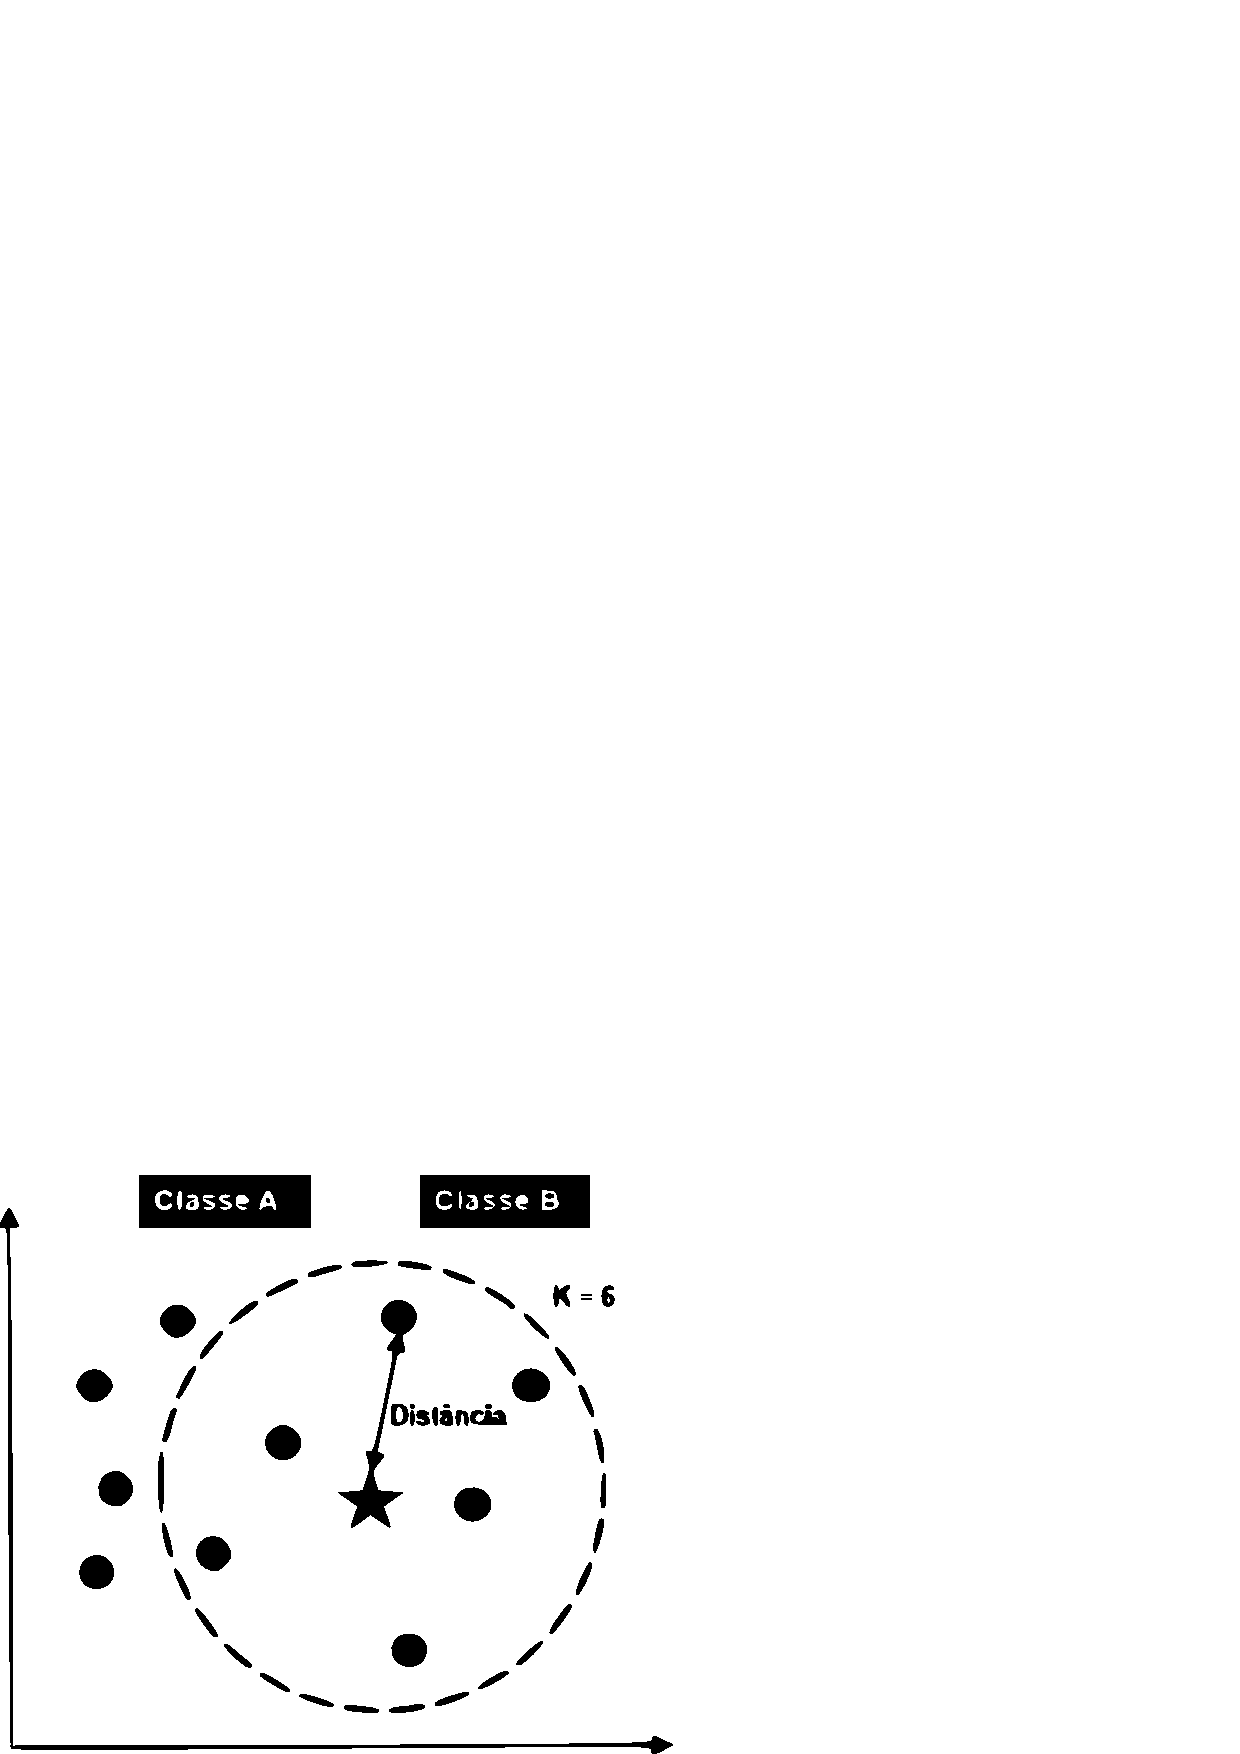
\includegraphics[scale=0.9]{imgs2/knn.png}
\source{Jonas Mendonça Targino, 2018}

\label{fig:knn}
\end{figure}


A literatura apresenta muitas aplicações usando KNN, como o diagnóstico de câncer de mama \cite{Sarkar_2000}, a classificação de texto \cite{Yu_2007} e \cite{Han_2001}, reconhecimento de emoção \cite{Cheng_2008}, identificação de falante \cite{Kacur_2011} , entre muitos outros. 

Uma das principais fraquezas do classificador KNN é que todas as amostras de treinamento devem ser armazenadas na memória e, para realizar a classificação, é necessário o cálculo da distância da amostra de teste para todas as amostras de treino.  À medida que o número de amostras no conjunto de treinamento aumenta, armazenar todos os seus valores na memória do computador pode não ser viável e também o procedimento de classificação pode levar muito tempo devido o cálculo das distâncias.


%\section{Rede Neural MLP}
%Uma rede neural é uma estrutura computacional inspirada no estudo do processamento neural biológico. Existem muitos tipos diferentes de redes neurais, de relativamente simples a muito complexas, assim como existem muitas teorias sobre o funcionamento do processamento neural biológico. Uma rede neural de alimentação avançada em camadas tem camadas ou subgrupos de elementos de processamento. Uma camada de elementos de processamento faz cálculos independentes em dados que recebe e passa os resultados para outra camada. A próxima camada pode, por sua vez, fazer seus cálculos independentes e transmitir os resultados para outra camada. Finalmente, um subgrupo de um ou mais elementos de processamento determina a saída da rede. Cada elemento de processamento faz seu cálculo com base em uma soma ponderada de suas entradas. A primeira camada é a camada de entrada e a última camada de saída. As camadas que são colocadas entre as primeiras e as últimas camadas são as camadas ocultas. Os elementos de processamento são vistos como unidades que são semelhantes aos neurônios em um cérebro humano e, portanto, são referidas como células ou neurônios artificiais. Uma função de limite é às vezes usada para qualificar a saída de um neurônio na camada de saída. As sinapses entre neurônios são referidas como conexões, que são representadas por bordas de um gráfico direcionado em que os nós são os neurônios artificiais. As redes neurais consistem em pequenas unidades chamadas neurônios, e estas estão conectadas entre si de tal maneira que podem passar sinais uns dos outros \cite{Askarunisa_2009}.
%
%Um percorridor de camada única avançado treinado com Back-propagation e Levenberg-Marquardt algoritmo \cite{haykin_2009}, foi usado neste trabalho. O algoritmo Back-propagation usado no treinamento de perceptron multicamada, é formulado como um problema não linear de mínimos quadrados. Essencialmente, o algoritmo de Levenberg-Marquardt é um método de estimativa de mínimos quadrados baseado na ideia máxima de vizinhança. Deixe $ E (w) $ ser uma função de erro objetivo composta de $ m $ termos de erro individual $ e_i ^ 2 (w) $ como segue:
%\[E (w) = \ sum_ {i = 1} ^ m e_i ^ 2 (w) = || f (w) || ^ 2 \]
%Em que
%\[e_i ^ 2 (w) = (y_ {i} -y_ {ri}) ^ 2 \]
%$ y_ {i} $ é o valor desejado do neurônio de saída $ i $ e $ y_ {ri} $ é a saída real desse neurônio. Supõe-se que a função $ f (.) $ E o Jacobiano $J$ são conhecidos no ponto $ w $. O objetivo do algoritmo Levenberg-Marquardt é calcular o vetor de peso $ w $, de modo que $ E (w) $ seja mínimo. Em cada iteração, o vetor de peso é atualizado de acordo com (\ ref {eq: atualizaw}).
%
%\begin{equation}
%\label{eq:atualizaw}
%w_{k+1}=w_k + \delta w_k
%\end{equation}
%em que
%\begin{equation}
%\label{eq:gradiente}
%\delta w_k = - (J_k^Tf(w_k))(J_k^TJ_k+ \lambda I)^{-1}
%\end{equation}
%$ J_k $ é a jacobiana de $ f (.) $ Avaliado em $ w_k $, $ \lambda $ é o parâmetro Marquardt e $ I $ é a matriz de identidade.
%
%
%
%
%\section{Floresta de caminhos ótimos}
%Ao contrário do k-NN, o OPF é um classificador muito recente proposto nos anos 2000 por \cite{Papa_2009a}. Não é paramétrico, rápido, simples, multi-classe, não faz qualquer suposição sobre as formas das classes e pode lidar com qualquer grau de sobreposição entre classes \cite{Papa_2009a}. O OPF foi usado com sucesso em muitas aplicações, como a detecção de patologia laríngea \cite{Papa_2008}, reconhecimento de face \cite{Papa_2009b}, estimativa de chuva \cite{Freitas_2009}, categorização de imagem \cite{Papa_2011}, entre muitos outros.
%
%
%O OPF é uma técnica de classificação baseada em gráficos, sendo responsável pela redução, para classificar cada classe, ou seja, o protótipo de acordo com uma ou mais árvores. Portanto, cada nó do gráfico representa uma amostra do conjunto de treinamento atuando mais especificamente como o descritor, pertencente à árvore do protótipo, na medida em que é maior grau de conexão de acordo com as bordas que são as distâncias entre os descritores.




\section{Máquina de aprendizado extremo}
\label{sec:ELM}

Máquina de Aprendizado Extremo é um algoritmo de classificação proposto por  \cite{Huang_2006} e \cite{Huang_2009}. A ELM é uma rede neural artificial (RNA) com uma única camada oculta, essa estratégia vem alcançando sucesso no contexto de classificação e regressão. 

A ELM possui o mesmo princípio de funcionamento de uma RNA,   diferenciando-se da MLP e RBF por sua metodologia de treinamento que não é baseada em gradientes. Isso deve-se ao fato que a ELM atualiza apenas os pesos da camada escondida. Já os pesos da camada de entrada são escolhidos aleatoriamente e fixados, isso permite a essa estratégia escapar das principais deficiências do algoritmo de treinamento \textit{backpropagation}. Possibilitando velocidade de aprendizado significativamente rápida, quando comparada a redes neurais MLP e RBF, assim como também proporciona menor intervenção humana do que outros algoritmos. Outro ponto é a facilidade e rapidez na implementação quando comparada a implementação de outros classificadores tradicionais.

A ELM pode determinar analiticamente todos os parâmetros de uma rede neural MLP em vez de ajustar parâmetros iterativamente. Assim, podendo superar algumas das dificuldades do método baseado em gradientes e da maioria dos outros métodos de aprendizagem. O trabalho de \cite{Huang_2006} também mostra que a ELM tende alcançar melhores resultados de generalização do que técnicas de classificação como SVM. Outro fator importante da ELM é sua baixa sensibilidade aos parâmetros especificados pelo usuário. Na figura \ref{fig:ELM} é possível visualizar a estrutura de uma ELM.

\begin{figure}[H]
\centering
\caption{Estrutura de uma Rede Neural ELM}
\includegraphics[scale=0.60]{imgs/ELM.png}
\source{Jonas Mendonça Targino, 2018}
\label{fig:ELM}
\end{figure}



No treinamento da ELM a matriz \textbf{W} (pesos da camada de entrada) é gerada de maneira aleatória e é inalterada. Portanto, o objetivo do treinamento da ELM é encontrar a matriz de pesos $\beta$, que são os pesos da camada oculta, baseado na matriz de saída \textbf{Y} e na matriz de pesos aleatórios \textbf{W}, por meio da resolução de um sistema linear. 

Com essa finalidade, a primeira ação é determinar \textbf{H}, que é a matriz que contem a função de ativação (podendo ser sigmóide, tangente hiperbólica, e etc.) dos neurônios da camada oculta.  Portanto, a matriz \textbf{H} armazena o resultado de todos os neurônios da camada oculta obtidos a partir da multiplicação entre \textbf{X} e \textbf{W}. Após determinada a matriz \textbf{H}, para se obter os pesos da matriz $\beta$ deve ser solucionado o sistema linear presente na equação \ref{eq:pinv}.


\begin{equation}
H = f_{ativ}(X\cdot W) \Rightarrow H\boldsymbol{\mathbf{\beta}} = Y \Rightarrow \mathbf{\mathbf{B}} = pinv(H)\cdot Y
\label{eq:pinv}
\end{equation}

Em que $f_{ativ}$ é a função de ativação e \textit{pinv} é pseudo inversa da matriz H. 



\section{Máquina de vetores suporte}
\nomenclature{SVM}{Support Vector Machines}
A Máquina de Vetores Suporte \cite{cortes1995support}  funciona da seguinte forma: dado um conjunto de dados de treinamento composto de \textit{N} amostras $\{x_i, y_i \}_{i = 1} ^ N $ com entrada $ x_i \in \mathcal{R}^n$ e saída $y_i \in \pm 1 $, o classificador SVM visa construir uma superfície de decisão da forma $ sign [f (x; w)] $, em que 
$ f (x; w) = w ^ T \phi (x) + b $
é uma aproximação da função de mapeamento $ y $, $ w \in \mathcal {R} ^ m $ e $ \ phi (.): \mathcal {R}^n \rightarrow \mathcal {R}^m $ is uma função que mapeia a entrada para um espaço de recurso de dimensão superior chamado. O parâmetro $ w $ e $ b $ podem ser obtidos por meio do seguinte problema de otimização \cite{Vapnik}:

\begin{equation}
\label {eq: rule1}
\min_ {w, b, \xi} \Phi (w, b, \xi) = \frac{1}{2} (w^Tw) + C \sum_ {i = 1} ^ N \xi_i,
\end{equation}

\noindent sujeito a $ y_i [w ^ T \phi (x_i) + b]\ geq 1 - \xi_i, \xi_i \geq 0, i = 1, \cdots, N $, em que $ C $ é um \textit{trade-off} parâmetro que indica a importância relativa da complexidade do modelo quando comparado ao erro de treinamento e $ \xi_i $ é o erro de treinamento para a amostra $ i $ -th.
Por simplicidade, o problema (\ref{eq: rule1}) geralmente é convertido em um problema equivalente definido em um espaço duplo, construindo o seguinte Lagrangiano \cite{Vapnik}: $ L (w, b, \xi, \beta, \gamma) $.

\begin{equation}
\frac {1} {2} w ^ Tw + C \sum_ {i = 1} ^ N \xi_i- \sum_ {i = 1} ^ N \beta_i \{[w ^T \phi (x_i) + b] y_i-1 + \ xi_i \} - \sum_{i = 1} ^ N \gamma_i \ xi_i
\end{equation}

\noindent em que $ \beta_i \geq 0 $, $ \gamma_i \geq 0 $, $ (i = 1, \cdots, N) $ são multiplicadores Lagrange. Em tal informação, um determinado tipo de função, conhecido como kernel, é empregado \cite{Scholkopf}. Deve seguir a restrição imposta pelo Teorema de Mercer e fornece um cálculo implícito de um passo do produto entre $ \phi (x_i) $ e $ \ phi (x_j) $: $ K (x_i, x_j) = <\phi (x_i), \phi (x_j)> $. Os resultados discutidos na Seção \ ref {seg: resultados} foram obtidos com o Kernel RBF: $ K (x_i, x_j) = exp \left (- \frac {(x_i-x_j) ^ T (x_i-x_j)} {2 \sigma ^ 2} \right) $, em que $ \sigma ^ 2 $ indica a variância a ser definida pelo usuário. Usando o Kernel, $f(x; w) $ podem ser reescritos como
$ f (x; w) = \sum_{i = 1} ^ N \beta_iy_iK(x, x_i) + b $.

Para as amostras de treino ao longo do limite de decisão, os correspondentes $ \alpha_i $ são maiores do que zero, conforme estabelecido pelo teorema de Karesh-Kuhn-Tucker. Essas amostras são conhecidas como vetores de suporte. O número de vetores de suporte geralmente é muito menor que $ N $, sendo proporcional ao erro de generalização do classificador. O vetor de teste $ {x}$ em $ {R} ^ m $ é atribuído a uma determinada classe de acordo com $ f(n) = sign [\mathbf {w} ^ T \phi (\mathbf {x}) + b] = sign(\sum_ {i = 1} ^ {N} \alpha_iy_iK (\mathbf {x}, \mathbf {x_i}) + b) $.  Podemos visualizar o problema de classificação binário por meio da figura \ref{fig:svm}.

\begin{figure}[H]
\centering
\caption{Problema de classificação binário com SVM}
\includegraphics[scale=0.60]{imgs/svm}
\source{Jonas Mendonça Targino, 2018}
\label{fig:svm}
\end{figure}


\section{Considerações finais do capítulo}

Existe uma quantidade considerável de classificadores e extratores presentes na literatura, entretanto neste trabalho foi utilizada a Transformada Wavelet como extrator de características, enquanto como classificadores utilizou-se K-vizinhos mais próximos, Máquina de Aprendizado Extremo e Máquinas de Vetores de Suporte. 
 %ok 
\include{proposta} % ok
\include{experimentos} %ok 
\include{conclusao} %ok 
\bibliography{referencias} % ok

\begin{apendicesenv}
%\begin{apendicesenv}

\chapter{Protocolo de revisão sistemática sobre técnicas para detecção e reconstrução de olusões parciais em imagens de face}
\label{apen2:RS}

\section{Objetivo}



O objetivo principal dessa revisão sistemática foi realizar um levantamento sistemático do estado de arte, referente a técnicas de detecção e reconstrução de oclusões parciais em imagens de faces humanas visando o reconhecimento biométrico. Mediante esse estudo, foi possível extrair dados para o tema desta dissertação, a fim de conseguir informações pertinentes, como por exemplo: quais algoritmos estão sendo aplicados para detectar oclusões parciais, e reconstruir faces parcialmente ocluídas, quais as métricas de avaliação que são normalmente utilizadas, quais estratégias estão apresentando melhor resultado, quais as condições do ambiente, e quais bases de dados utilizadas.


% ----------------------------------------------
\section{Questões de pesquisa}
Em adição aos objetivos da revisão sistemática elaborada, as questões de pesquisa auxiliam na busca por informações relevantes por meio da leitura integral dos estudos. Tais informações são obtidas após a extração e síntese dos dados extraídos da leitura. As questões de pesquisa levantadas foram:

\begin{enumerate}
\item quais técnicas estão sendo utilizadas para reconstrução de faces humanas e como são aplicadas?	
\item quais as técnicas utilizadas para detecção de oclusões parciais e como são aplicadas?
 \item como os resultados são analisados e comparados?
 \item qual tipo de reconhecimento biométrico foi utilizado?\item Quais bases de dados estão sendo utilizadas?
\end{enumerate}
%---------------------------------------------------

\section{Seleção de fontes}
Para selecionar os estudos primários para essa revisão sistemática, foram utilizadas as três bases indexadoras a seguir:

Os trabalhos devem estar preferencialmente disponíveis na internet, em bases de dados científicas. As seguintes bases foram selecionadas para realização das buscas:

\begin{enumerate}
\item Biblioteca Digital do Scopus (https://www.scopus.com/)
\item Biblioteca Digital do IEEE (http://ieeexplore.ieee.org/Xplore/home.jsp)
\item Biblioteca Digital do Web of Science (https://apps.webofknowledge.com)
\end{enumerate}

A justificativa para a escolha dessas três bases se refere à abrangência, quase total, dos artigos presentes nas bibliotecas digitais com idioma na língua inglesa. Para encontrar tais artigos nas bases indexadoras, foi elaborado uma string de busca para cada uma das bases com os termos descritos mais detalhadamente na seção \ref{ap:palavraschave}. O apêndice \ref{Apen:conducao_Revisao}, apresenta com maiores o processo de seleção de artigos.


%----------------------------------------------------

\section{Palavras-Chave}
\label{ap:palavraschave}
A \textit{String de busca} envolveu as palavras-chave descritas abaixo:

\begin{enumerate}
\item 'occlusion' OR 'occluded';
\item 'detect*' OR 'recogni*' OR 'analys*' OR 'reconstruct*';
\item 'face' OR 'faces' OR 'facial' ;
\item 'biometry*'.
\end{enumerate}

Os artigos retornados pela aplicação da \textit{String} de busca nos motores de busca, foram lidos seus respectivos títulos e resumos.
% -------------------------------------------

\section{Critérios de inclusão}
Para essa revisão sistemática, três critérios de inclusão foram definidos, sendo eles:

I1 - Artigos que abordem métodos e técnicas utilizadas para detecção de oclusão parciais em faces humanas.

I2 - Artigos que abordem técnicas utilizadas para reconstrução de faces humanas.

I3 - Artigos que abordem modelagens híbridas para detecção de oclusões parciais e/ou reconstrução facial. 

%--------------------------------------------

\section{Critérios de exclusão}


E1 - Artigos de revisão serão excluídos.

E2 - Trabalhos que estejam na forma de livros, capítulos de livros, prefácio de eventos, pôster e artigos resumidos.

E3 - Trabalhos que não estejam na língua Inglesa.

E4 - Trabalhos que não sejam revisados por pares.

% -----------------------------------------------

\section{Estratégia de seleção dos dados}

Foi construída uma \textit{String} com palavras-chave e seus sinônimos, onde essa \textit{String} foi submetida nas máquinas de busca. Após a leitura dos resumos e títulos e sua posterior aplicação dos critérios de inclusão e exclusão, com isso os artigos foram selecionados conforme sua adequação juntos aos critérios de inclusão, apresentando relevância daquele artigo perante a pesquisa. 

%------------------------------------------------

\section{Síntese dos dados extraídos}

Após a leitura na íntegra de cada artigo incluído, foi elaborado um formulário de extração dos dados, a fim de serem sintetizados e gerar informações pertinentes, os dados coletados foram:

\begin{enumerate}
\item autores;
\item objetivo do trabalho;
\item estratégia para detecção de oclusão parcial;
\item estratégia para reconstrução de face;
\item base de dados utilizada;
\item forma de avaliação;
\item métricas utilizadas;
\item identificação das vantagens e desvantagens de cada método;
\item resultados obtidos;
\item limitações do trabalho;
\item trabalhos futuros.

\end{enumerate}


\section{Ameaças a validade}


Os resultados da pesquisa podem revelar que as técnicas ou fusões de técnicas apresentadas para detecção de oclusão ou reconstrução de faces não produzem um bom resultado ou não são aplicáveis a tal ambiente de coleta, assim refutando a hipótese de pesquisa. 
Outra possível ameaça que este projeto pode apresentar é a existência de outras técnicas com fins a identificar a parte ocluída em uma imagem facial e/ou reconstruir a face sem finalidades biométricas.


\section{Critérios de qualidade}
Após a seleção dos estudos e a leitura integral de cada um deles, existe a necessidade de realizar uma avaliação subjetiva direcionada ao objetivo da revisão sistemática. Desse modo, alguns critérios de qualidade foram desenvolvidos para tal fim, sendo eles:


Q1 -	Os objetivos da pesquisa são claramente definidos?

Q2 -	O contexto é adequadamente descrito?

Q3 - 	Foram apresentadas técnicas de detecção de oclusões claramente?

Q4 -	Foram apresentadas técnicas de reconstrução facial?

Q5 -	O código de detecção de oclusões foi disponibilizado?

Q6 - 	O código de detecção de reconstrução facial foi disponibilizado?

Q7 -	O ambiente do estudo primário foi apresentado claramente?

Q8 -	A proposta do estudo foi validada?

Q9 -	A proposta é comparada com outro método?

Q10 -	 Foi apresentado o Dataset utilizado?

Q11 - 	 O experimento é aplicado em conjuntos de dados suficientes?

Q12 -	 Os resultados foram apresentados claramente?

Para cada critério de qualidade necessariamente era atribuído uma nota, sendo Sim (S) = 1 ponto, Não (N) = 0 ponto, e Parcialmente (P) = 0,5.



\chapter{Condução da revisão}
\label{apen3:conducao_Revisao}


Após o planejamento da revisão sistemática e definição do protocolo, a condução dos passos consistiram das seguintes etapas: submissão das \textit{strings} nas máquinas de busca do Scopus, IEEE e Web of Science; aplicação dos artigos retornados nas máquinas de busca e aplicação dos critérios de inclusão e exclusão; e extração dos dados dos artigos incluídos e lidos integralmente.

O processo de busca dos artigos foi realizado no período compreendido entre 25 de janeiro e 06 de fevereiro de 2017. A partir dessas buscas 440 artigos foram retornados, de modo que após a aplicação dos critérios de inclusão e exclusão 38 artigos foram selecionados para leitura e análise completa, sendo que após a leitura completa do trabalho foram selecionados 31 artigos com relevante grau de contribuição para a pesquisa. A figura \ref{fig:esquemaconducao} apresenta um esquema do processo de seleção dos artigos.

\begin{figure}[H]
\caption{Processo de seleção dos artigos}
\centering
\includegraphics[scale = 0.65]{imgs/conducao.png}
\source{Jonas Mendonça Targino, 2018}
\label{fig:esquemaconducao}
\end{figure}





\chapter{Contextualização da literatura}
\label{apen4:contextualizacao_literatura}


Este  capítulo possui como objetivo principal apresentar um apanhado geral das técnicas para detecção e reconstrução de oclusões parciais em imagens de face visando o reconhecimento biométrico. Essas técnicas foram obtidas graças ao trabalho de \citeonline{Targino2018_wvc} o qual apresentou uma revisão sistemática das técnicas presentes na literatura. 


\section{Escopo dos estudos}

Dentro do conjunto de estudos selecionados e analisados, existem autores que abordam a técnica de detecção de oclusão e paralelamente realizam a reconstrução da face, entretanto em outros trabalhos são implementados apenas uma das duas técnicas. Diante dos trabalhos lidos foi possível perceber que a maioria deles não apresentaram o algoritmo de construção da técnica de forma detalhada. Sendo possível a implementação da técnica mediante a leitura de outros trabalhos com abordagens semelhantes e mais específicas, abrangendo com isso uma maior quantidade de detalhes. É notável perceber que a maioria dos trabalhos abordaram adaptações de técnicas já existentes para detecção e reconstrução de oclusões parciais. 



\section{Bases de dados}
\label{sec:base de dados}

Três bases de dados foram amplamente utilizadas nos trabalhos analisados e esta seção as descreve resumidamente. Em alguns artigos mais de uma base foram utilizadas de modo a possibilitar o uso de uma ou mais bases para o conjunto de treinamento e outra de modo a prover instâncias para o conjunto de teste. Todas as bases de dados utilizadas nos trabalhos abordados na revisão sistemática estão representadas na figura \ref{fig:basesDeDados}, dentre essas apresentadas, aqui será dado maior ênfase nas três bases de dados mais utilizadas, sendo elas:

\begin{itemize}
\item \textbf{AR} esta base de dados foi utilizada em nove dos trabalhos analisados (29\%). Ela possui um pouco mais de 2.600 imagens de face frontal de 100 indivíduos (50 homens e 50 mulheres). De modo que para cada indivíduo são coletadas 26 fotos, estas coletadas sobre duas sessões (dois dias diferentes) separadas e sujeitas a 13 variações de condições, dentre estas estão, diferentes expressões faciais, condições de iluminação e variações de oclusão (com óculos de sol e cachecol). A base de dados encontra-se disponível em \url{http://www2.ece.ohio-state.edu/~aleix/ARdatabase.html};

\item \textbf{YALE B} esta base de dados contém 165 imagens frontais de 10 pessoas, contendo variações de iluminação, expressão e oclusão (baixos níveis de oclusão). A base de dados foi utilizada em quatro dos trabalhos selecionados (14\%), e ela encontra-se disponível em \url{http://www.face-rec.org/databases/};

\item \textbf{FRGC} foi a terceira base de dados mais utilizada, três dos trabalhos analisados (11\%) a utilizaram. Esta base de dados contém 12776 imagens frontais de 222 indivíduos, com 6388 imagens coletadas em ambientes controlados e outras 6388 imagens coletadas na presença de ambientes não controlados. Esta base de dados está disponível em \url{https://www.nist.gov/programs-projects/face-recognition-grand-challenge-frgc}.

\end{itemize}

\begin{figure}[H]
\centering
\caption{Bases de dados utilizadas pelos estudos selecionados}
\includegraphics[scale = 0.62]{imgs/bases.png}
\source{Jonas Mendonça Targino, 2018}
\label{fig:basesDeDados}
\end{figure}


Pode-se perceber uma quantidade significativa de bases de dados de face dispostas na literatura, entretanto nem todas as bases disponíveis apresentam uma grande quantidade de imagens bem como também uma grande quantidade de variações existentes. Na tabela \ref{tab:variacoes_bases} são apresentadas algumas das bases mais utilizadas como também número de indivíduos da base, quantidade de imagens, e variações presentes na base. As variações estão apresentadas da forma: (\textbf{i}) representa iluminação; \textit{e} significa expressão; (\textbf{o}) representa oclusão; e \textbf{t} significa variação temporal (ou seja, imagens obtidas da mesma pessoa em diferentes dias).

\begin{table}[H]
	
\centering
\footnotesize
\caption{Bases de dados de domínio público e algumas especificações}
\label{tab:variacoes_bases}

\begin{tabular}{|l|c|c|c|} \hline

\textbf{Bases}& \textbf{Número de indivíduos} & \textbf{Número de imagens} & \textbf{Variações existentes}\\ \hline
      					
AR			&	 100 	& 2600 		& i, e,o, t \\ \hline
Yale B	 	&	15 		& 165 		& i,e\\ \hline
FRGC  		&	222 	& 12776 	& i,e \\ \hline
ORL 		&	40 		& 400 		& p,e\\ \hline
MIT 		&	16 		& 432		& i,p\\ \hline
CMU PIE 	&	68		&41.368 	& p,i,e\\ \hline
FERET		& > 1000 	& > 10000 	& p,i,e,t\\ \hline 
UMIST		& 20		& 564		& p \\ \hline 

		
	\end{tabular}
    
 \source{Jonas Mendonça Targino, 2018}
\end{table}


\section{Técnicas encontradas na literatura}

Após a extração dos dados foi possível analisar as técnicas presentes na literatura para detecção e reconstrução de oclusões parciais com fins biométricos, estas técnicas estão sendo apresentadas com mais detalhes nas subseções \ref{sub:detecção de oclusões} e \ref{sub:reconstrução de faces} logo abaixo.

De modo a gerar uma melhor visualização dos trabalhos selecionados e uma identificação para cada um deles foi elaborada o quadro \ref{tab:autores}, este apresentando a identificação do trabalho, como também o evento em que o mesmo foi publicado.


\begin{quadro}[H]
	\centering
	\caption{Estudos selecionados}
    \resizebox{\columnwidth}{!}{%
		\begin{tabular}{cll} \hline
        %\begin{tabular}{ p{0.2in} p{1.8in}  p{4.7in}   } \hline
		ID	& Autores  & Evento\\ \hline

A1& \cite{[1]bellil2016gappy}  & Multimed Tools Applications\\
A2 & \cite{[2]zhang2016face}  & Chinese Conference on Biometric Recognition\\
A3& \cite{[3]dou2015pose} & Biometrics Theory, Applications and Systems (BTAS)\\
A4 & \cite{[4]wei2014dynamic}  & IEEE Transactions on Information Forensics and Security\\
A5 & \cite{[5]aisha2014face} & KSII Transactions on Internet and Information Systems (TIIS)\\
A6 & \cite{[6]yang2014fast}   & Pattern Recognition\\
%A7 & \cite{[7]venkatakrishnan20143d} & 2014 & periódico & Applied Mechanics \& Materials\\
A7 & \cite{[8]alyuz2014detection}  & International Conference Pattern Recognition (ICPR) \\
A8& \cite{[9]bindu2014inpainting}   & Signal and Image Processing (ICSIP)\\
%A10 & \cite{[10]bindu2013novel} & 2013 & conferência & Advances in Computing, Communications and Informatics (ICACCI)\\
A9 & \cite{[11]lai2013robust}  & International Conference Acoustics, Speech, and Signal Processing (ICASSP)\\
A10  & \cite{[12]sharma2013efficient}& Neurocomputing\\
A11 & \cite{[13]wei2013robust} & International Workshop Biometrics and Forensics (IWBF)\\
A12 & \cite{[14]alyuz20133}  & IEEE Transactions on Information Forensics and Security\\
A13 & \cite{[15]li2013structured}  & IEEE transactions on image processing\\ 
A14 & \cite{[16]min2012inpainting}   & International Conference Image Processing (ICIP)\\
A15 & \cite{[17]alyuz2012robust}  & International Conference Biometrics (ICB)\\
A16 & \cite{[18]zhu2012discriminant} & International Conference Biometrics (ICB)\\
A17 & \cite{[19]song2012three} & IEEE Transactions on Image Processing\\
A18 & \cite{[20]shermina2012recognition}  & International Journal of Pattern Recognition and Artificial Intelligence\\
%A21 & \cite{[21]min2011cap} & 2011 & conferência & Proceedings of the 19th ACM international conference on Multimedia\\
A19 & \cite{[22]chiang2011recognizing}  & International Journal of Innovative Computing, Information and Control\\
A20 & \cite{[23]eum2011face} & Computer Vision and Pattern Recognition Workshops \\
A21 & \cite{[24]passalis2011using}& IEEE Transactions on Pattern Analysis and Machine Intelligence\\
A22 & \cite{[25]deng2011graph}   & IEEE Transactions on Image Processing\\
A23 & \cite{[26]storer2010occlusion}  & Computer Vision and Pattern Recognition Workshops (CVPRW)\\
A24& \cite{[27]yan2010misalignment}& IEEE transactions on image processing\\
A25 & \cite{[28]de2010faro}& IEEE Transactions on Systems, Man, and Cybernetics-Part A: Systems and Humans\\
%A29 & \cite{[29]marcon20093d} & 2009 & conferência & IET\\
%A30 & \cite{[30]du2009analysis} & 2009 & conferência & Information Technology and Applications\\
A26 & \cite{[31]su2009multi}  & International Conference on Biometrics\\
A27 & \cite{[32]wright2009robust}   & IEEE transactions on pattern analysis and machine intelligence\\
%A33 & \cite{[33]heo2007face} & 2007 & conferência & Biometrics Symposium\\
A28 & \cite{[34]zhang2006robust}  & Journal of Multimedia\\
%A35 & \cite{[35]lee2006face} & 2006 & conferência &International Conference Pattern Recognition (ICPR)\\
A29 & \cite{[36]huang2012subface}  & IET biometrics\\
A30 & \cite{[37]hosoi2012restoring} & Computer Vision and Pattern Recognition Workshops (CVPRW)\\
A31 & \cite{[38]tan2005recognizing}  &IEEE Transactions on Neural Networks\\
\hline
		\end{tabular}
        }
        \source{Jonas Mendonça Targino, 2018}
            \label{tab:autores}

\end{quadro}





\subsection{Técnicas para detecção de oclusões parciais}
\label{sub:detecção de oclusões}
Algumas técnicas para detecção de oclusões parciais em imagens de face, coletadas a partir da revisão sistemática estão destacadas no quadro \ref{tab:Tecnicas deteccao}. Após a análise deste quadro podemos enxergar um número considerável de técnicas com tal finalidade.



\nomenclature{IKFDA}{Incremental Kernel Fisher Discriminant Analysis}
\begin{quadro}[H]
	\centering
	\caption{Técnicas para detecção de oclusão}
		\begin{tabular}{p{1.2in} p{4.2in} } \hline

		ID do Artigo  & Nome da Técnica\\ \hline
  
A1& Transformada Wavelet Discreta(DCT) \nomenclature{DCT}{Discrete Wavelet Transform} \\
A2 & Rede Neural Convolucional(CNN) \nomenclature{CNN}{Convolucional Neural NetWork}   \\\
A4,A11& Imagens Dinâmicas para Classes Deformadas(DICW) \nomenclature{DICW}{Dynamic image to class Warping}\\
A5 & Kernel Incremental de Análise Discriminante de Fisher (IKFDA)  \\
A6,A25,A32 & Classificação por Representação Esparsa (SRC)  \nomenclature{SRC}{Sparse Representation  Classification} \\
A14 & Máscara de Projeção FisherFace\\
A7 & Mistura de Modelos Gaussianos (GMM) \nomenclature{GCC}{Gaussian Mixture Models} \\
%A10 & Skin ilumination e SURF\\
A9 & Classificação de regressão linear aparada (TLRC) \nomenclature{TLRC}{trimmed linear regression
classification} \\
A10 & Filtros de Gabor\\
A13 & Estrutura Esparsa de Codificação do Erro(SSEC) \nomenclature{SSEC}{Structured Sparse Error Coding}\\  
A14 & Robusta Análise dos Componentes Principais (RPCA) \nomenclature{RPCA}{Robust Principal Component Analisys} \\
A15 & ICP junto ao modelo genérico facial\\
A16 & Fases de Gabor com SLRDA\\
A18 &  Bloco de Algoritmo de correspondência (BMA) \nomenclature{BMA}{Block Matching Algorithm}\\
%A21 & Skin color com DTW\\
A19 & Descoberta Iterativa de Faces(IFR) \nomenclature{IFR}{Iterative Face Recovery}\\
A20& Manipulação de Oclusões Excepcionais(EOH) \nomenclature{EOH}{Exceptional Occlusion Handling}\\
%A21 & UR3DS\\
A23 & Técnica do Espaço de Cores (CST) \nomenclature{CST}{Color Space Technique}\\
A24 & Desalinhamento Robusto (MAR)\\
A25 & Reconhecimento Facial contra Oclusão(FARO)\nomenclature{FARO}{Face Recognition Against Occlusion}\\
%A30 & Skin color\\
A26 & Multi Visões de Alinhamento de Faces \\
A28 & Memória de Kernel Associativo(KAM) \nomenclature{KAM}{Kernel Associative Memory}\\
A29 & Modelos Ocultos Markovianos (HMM) \nomenclature{HMM}{Hidden Markov Models}\\
A31 & Mapa de Auto Organização(SOM) \nomenclature{SOM}{Self Organizaton Maps}\\

 \hline
		
		\end{tabular}
		\source{Jonas Mendonça Targino, 2018}
	\label{tab:Tecnicas deteccao}
\end{quadro}

	


\subsection{Técnicas para reconstrução de imagens de Faces}
\label{sub:reconstrução de faces}

Após a fase de detecção da oclusão na imagem da face, torna-se imprescindível a reconstrução da oclusão, de modo a possibilitar a identificação biométrica. A partir da leitura dos artigos foi possível extrair algumas técnicas para reconstrução de faces. As técnicas encontradas são apresentadas no quadro \ref{tab:Tecnicas reconstrução}. Analisando este quadro pode-se perceber um pequeno número de técnicas com tal finalidade quando comparado com as técnicas para detecção de oclusão. 


\begin{quadro}[H]
	\centering
	\caption{Técnicas para reconstrução de faces}
		\begin{tabular}{p{1.1in} p{4.4in} } \hline

		ID do Artigo & Nome da Técnica\\ \hline
  
A1 & Rede Neural de Onda de Multi-Biblioteca (MLWNN) \nomenclature{MLWNN}{Multi Library Wavelet Neural Network} \\
%A3 & 3DAFM\\
A4,A27 & SRC\\
A7 & Inpainting for big data (IBD) \nomenclature{IBD}{Inpainting for Big Data}\\
A9 & TLRC\\
A10 & Eigenfaces com Eigenfaces reformados de Gabor(RGEF)\nomenclature{RGEF}{Reformed Gabor Eigen Faces} \\
A12,A15 & Gappy Análise dos Componentes Principais (GPCA) \nomenclature{GPCA}{Gappy Principal Component Analysis} \\
A16 & Fases de Gabor com RSLDA\\
%A17 & CRBF netwok \\ é aplicada apenas para 3D
A18,A19,A24 & Eigenfaces \nomenclature{PCA}{Principal Component Analysis} \\
A22 & Grafos Laplacianos\\
A23 & CST + Modelos de Formas Ativas (ASM) \nomenclature{ASM}{Active Shape Model} e PCA\\
A28 & KAM \\
A30 & Pesos Rápidos de Análises de Componentes Principais (FWPCA) \nomenclature{FWPCA}{Fast-Weighted Principal Component Analysis}\\
                
 \hline
		\end{tabular}
		\source{Jonas Mendonça Targino, 2018}
	\label{tab:Tecnicas reconstrução}
\end{quadro}



\section{Considerações finais do apêndice}

Considerando a importância das técnicas de detecção e reconstrução de oclusões parciais em imagens de face visando o reconhecimento biométrico. Neste apêndice foi apresentada uma revisão sistemática de literatura a respeito das técnicas presentes no estado da arte com fins de detecção e/ou reconstrução de oclusões parciais em imagens de de face.

Com a análise dos artigos incluídos percebeu-se que existe uma quantidade considerável de técnicas presentes na literatura, entretanto essas técnicas apresentam configurações de execuções limitadas, não seguindo um rigor sistemático de bases de dados utilizadas, como também disponibilidade de códigos ou pseudo-códigos para futuras replicações por outras pessoas interessadas na área.

Foi possível concluir com essa revisão sistemática, que a área apresenta uma certa instabilidade em relação a padrões de execuções, tipos de oclusões, sem contar que alguns autores não utilizam um estudo comparativo mais aprofundado com outras técnicas presentes no estado da arte. Como também grande parte dos artigos não apresentam fins que possibilitem replicação do trabalho pela comunidade científica.


\chapter{Matrizes de confusão}
\label{apen6:matrizes_confusao}
Abaixo são apresentadas as matrizes de confusão de cada técnica, de modo que após a análise da diagonal é possível perceber qual classe teve um maior índice de acertos, como também seus falsos positivos e falsos negativos.

\section{Técnicas baseadas em subespaço}

\begin{figure}[H]
\caption{Matriz de confusão da técnica Asymmetrical PCA na base de dados AR}
\centering
\includegraphics[scale = 0.65]{imgs4/matrizes_confusao/APCA}
\source{Jonas Mendonça Targino, 2018}
\end{figure}

\begin{figure}[H]
\caption{Matriz de confusão da técnica Fast Recursive PCA na base de dados AR}
\centering
\includegraphics[scale = 0.65]{imgs4/matrizes_confusao/FastRecPCA}
\source{Jonas Mendonça Targino, 2018}
\end{figure}

\begin{figure}[H]
\caption{Matriz de confusão da técnica Fisherfaces na base de dados AR}
\centering
\includegraphics[scale = 0.65]{imgs4/matrizes_confusao/fisherfaces}
\source{Jonas Mendonça Targino, 2018}
\end{figure}


\begin{figure}[H]
\caption{Matriz de confusão da técnica Fast Robust PCA na base de dados AR}
\centering
\includegraphics[scale = 0.65]{imgs4/matrizes_confusao/FRPCA}
\source{Jonas Mendonça Targino, 2018}
\end{figure}

\begin{figure}[H]
\caption{Matriz de confusão da técnica Gappy PCA na base de dados AR}
\centering
\includegraphics[scale = 0.65]{imgs4/matrizes_confusao/GPCA}
\source{Jonas Mendonça Targino, 2018}
\end{figure}

\begin{figure}[H]
\caption{Matriz de confusão da técnica PCA na base de dados AR}
\centering
\includegraphics[scale = 0.65]{imgs4/matrizes_confusao/PCA}
\source{Jonas Mendonça Targino, 2018}
\end{figure}


\begin{figure}[H]
\caption{Matriz de confusão da técnica Recursive PCA na base de dados AR}
\centering
\includegraphics[scale = 0.65]{imgs4/matrizes_confusao/RecPCA}
\source{Jonas Mendonça Targino, 2018}
\end{figure}


\begin{figure}[H]
\caption{Matriz de confusão da técnica SRC com Fast Recursive PCA na base de dados AR}
\centering
\includegraphics[scale = 0.65]{imgs4/matrizes_confusao/src_fast_rec_PCA}
\source{Jonas Mendonça Targino, 2018}
\end{figure}




%%%%%%%%%%%%%%%%%%%%%%%%%%%%%%%%%%%%%%%%%%%%%%%%%%%
%%%%%%%%%%%%%%%%%%%%%%%%%%%%%%%%%%%%%%%%%%%%%%%%%%%
\section{Técnicas baseadas em modelo}



\begin{figure}[H]
\caption{Matriz de confusão da técnica SRC com grafo de Poisson na base de dados AR}
\centering
\includegraphics[scale = 0.65]{imgs4/matrizes_confusao/SRC_GP}
\source{Jonas Mendonça Targino, 2018}
\end{figure}



\begin{figure}[H]
\caption{Matriz de confusão da técnica SRC com grafo Laplaciano na base de dados AR}
\centering
\includegraphics[scale = 0.65]{imgs4/matrizes_confusao/SRC_GL}
\source{Jonas Mendonça Targino, 2018}
\end{figure}


\begin{figure}[H]
\caption{Matriz de confusão da técnica SSIMGL na base de dados AR}
\centering
\includegraphics[scale = 0.65]{imgs4/matrizes_confusao/ssimgl}
\source{Jonas Mendonça Targino, 2018}
\end{figure}

%\end{apendicesenv}




   %contém as partes da RS e as matrizes de confusão
\chapter{Tabelas de resultados}
\label{apen7:resultados}


\section{Resultados com a base ocluída}

Antes de apresentar a acurácia de reconhecimento das técnicas baseadas em subespaço e subespaço para a tarefa de reconstrução é interessante apresentar-se a acurácia de reconhecimento do classificador após aplicação da imagem pura com oclusão. Mediante isso os resultados abaixo apresentam o comportamento da taxa de reconhecimento das bases mediante avaliação com os classificadores KNN, ELM e SVM.


%
%\pdfbookmark[0]{\contentsname}{toc}
%\tableofcontents* %inserir o sumário
%\cleardoublepage
%\textual





\subsection{ELM nível LL3}

\begin{table}[H]
	\centering
    \normalsize
	\caption{Taxa de reconhecimento com ELM na base de dados AR com oclusões com nível de decomposição LL3}
    \label{tab:reconhecimento_AR_com_oclusoes}
   % \hspace{0.5in}
	\begin{tabular}{|c|c|c c c c c|}
\cline{3-7}
\multicolumn{2}{c|}{\multirow{3}{*}{}} & \multicolumn{5}{c|}{\textbf{AR\#1}}   \\\cline{3-7} 
\multicolumn{2}{c|}{}  & db2 & db4 & sym3 & sym4 & sym5 \\\cline{3-7}%& db2 & db4& sym3 & sym4 & sym5 \\\cline{3-12}
\multicolumn{2}{c|}{}& $\mu \pm \sigma$ & $\mu \pm \sigma$ & $\mu \pm \sigma$ & $\mu \pm \sigma$ & $\mu \pm \sigma$ \\\hline


\multicolumn{1}{|c|}{ \multirow{5}{*}{\rotatebox[origin=c]{90}{\textbf{Neurônios}}} }
& 200		&40.99$\pm$2.02	&39.53$\pm$2.98	&37.55$\pm$1.53		&37.68$\pm$1.74	&40.00$\pm$3.34 \\\cline{2-7}% 
& 500		&44.74$\pm$2.74	& 46.85$\pm$2.02&42.94$\pm$3.24		&45.89$\pm$1.82	&45.05$\pm$1.66 \\\cline{2-7}% 

& 1000		&25.10$\pm$1.65	&28.61$\pm$1.74	&26.87$\pm$1.92		&28.20$\pm$1.37	&26.65$\pm$1.61 \\\cline{2-7}% 

& 2000		&25.17$\pm$2.10	&29.88$\pm$2.15	&28.56$\pm$2.10		&29.13$\pm$1.59	&29.46$\pm$1.92 \\\cline{2-7}% 

& 4000		&41.33$\pm$1.81	&45.90$\pm$2.17	&44.20$\pm$1.32		&44.70$\pm$1.64	&43.38$\pm$2.27 \\\midrule% 

\multicolumn{7}{c}{}\\ 
%\toprule 
%%%%%%%%%%%%%%%%%%%%%%%%%%%

\cline{3-7}
\multicolumn{2}{c|}{\multirow{3}{*}{}} & \multicolumn{5}{c|}{\textbf{AR\#2}}   \\\cline{3-7} 

\multicolumn{2}{c|}{}  & db2 & db4 & sym3 & sym4 & sym5 \\\cline{3-7}
\multicolumn{2}{c|}{}& $\mu \pm \sigma$ & $\mu \pm \sigma$ & $\mu \pm \sigma$ & $\mu \pm \sigma$ & $\mu \pm \sigma$ \\\hline


\multicolumn{1}{|c|}{ \multirow{5}{*}{\rotatebox[origin=c]{90}{\textbf{Neurônios}}} }
& 200 &50.52$\pm$2.41	&47.00$\pm$2.42	&46.4$\pm$1.37	&45.30$\pm$2.83		&49.12$\pm$3.96 \\\cline{2-7}
&500  &53.62$\pm$3.58	&55.02$\pm$2.49	&52.12$\pm$4.75	&55.2$\pm$1.67		&54.85$\pm$3.29 \\\cline{2-7}
&1000 &30.97$\pm$2.72	&34.32$\pm$3.00	&32.52$\pm$2.34	&34.375$\pm$1.96	&32.22$\pm$2.84 \\\cline{2-7}
&2000 &30.22$\pm$3.39	&34.82$\pm$3.23	&33.62$\pm$3.09	&35.075$\pm$2.05	&35.22$\pm$2.28 \\\cline{2-7}
&4000 &46.67$\pm$2.65	&50.45$\pm$2.95	&49.75$\pm$2.19	&50.75$\pm$2.02		&48.47$\pm$2.55 \\ \midrule
\multicolumn{7}{c}{}\\ 



\cline{3-7}
\multicolumn{2}{c|}{\multirow{3}{*}{}} & \multicolumn{5}{c|}{\textbf{AR\#3}}   \\\cline{3-7} 

\multicolumn{2}{c|}{}  & db2 & db4 & sym3 & sym4 & sym5 \\\cline{3-7}
\multicolumn{2}{c|}{}& $\mu \pm \sigma$ & $\mu \pm \sigma$ & $\mu \pm \sigma$ & $\mu \pm \sigma$ & $\mu \pm \sigma$ \\\hline

\multicolumn{1}{|c|}{ \multirow{5}{*}{\rotatebox[origin=c]{90}{\textbf{Neurônios}}} }
&200	&39.83$\pm$2.30	&38.81$\pm$4.20	&32.08$\pm$3.85	&34.13$\pm$2.99	&39.20$\pm$5.01\\\cline{2-7} 

&500	&46.10$\pm$3.30	&51.51$\pm$2.68	&44.91$\pm$3.99	&46.76$\pm$3.20	&48.53$\pm$1.90 \\\cline{2-7} 

&1000	&31.85$\pm$2.46	&37.58$\pm$3.29	&35.80$\pm$3.48	&38.18$\pm$2.63	&35.86$\pm$2.59 \\\cline{2-7} 

&2000	&32.18$\pm$4.75	&39.75$\pm$3.51	&39.35$\pm$4.27	&41.90$\pm$2.33	&42.31$\pm$2.81 \\\cline{2-7}

&4000	&50.63$\pm$3.58	&57.10$\pm$2.89	&56.60$\pm$1.62	& 59.70$\pm$3.46&58.03$\pm$3.26 \\\midrule 
\multicolumn{7}{c}{}\\ 



\cline{3-7}
\multicolumn{2}{c|}{\multirow{3}{*}{}} & \multicolumn{5}{c|}{\textbf{AR\#4}}   \\\cline{3-7} 

\multicolumn{2}{c|}{}  & db2 & db4 & sym3 & sym4 & sym5 \\\cline{3-7}
\multicolumn{2}{c|}{}& $\mu \pm \sigma$ & $\mu \pm \sigma$ & $\mu \pm \sigma$ & $\mu \pm \sigma$ & $\mu \pm \sigma$ \\\hline

\multicolumn{1}{|c|}{ \multirow{5}{*}{\rotatebox[origin=c]{90}{\textbf{Neurônios}}} }
&200	&41.25$\pm$3.38		&39.36$\pm$3.42		&42.48$\pm$2.45	&40.65$\pm$3.18	&39.70$\pm$3.81  \\\cline{2-7}

&500	&42.43$\pm$4.09		&41.38$\pm$3.60		&40.75$\pm$3.85	& 44.21$\pm$1.44	&40.15$\pm$2.88 \\\cline{2-7}

&1000	&17.66$\pm$2.45		&18.96$\pm$1.71		&18.65$\pm$2.68	&17.93$\pm$2.89	&16.93$\pm$1.52 \\\cline{2-7}

&2000	&17.33$\pm$2.09		&19.38$\pm$1.82		&18.00$\pm$2.71	&16.31$\pm$2.44	&16.31$\pm$1.78 \\\cline{2-7}

&4000 &30.73$\pm$2.10		&33.16$\pm$2.87	&31.66$\pm$3.27	&29.65$\pm$2.12	&28.63$\pm$2.74 \\\midrule




	\end{tabular}
	\source{Jonas Mendonça Targino, 2018}
\end{table}














\begin{table}[H]
	\centering
    %\footnotesize
	\caption{Taxa de reconhecimento com ELM na base de dados Yale com oclusões com nível de decomposição LL3}
    \label{tab:reconhecimento_Yale_com_oclusao}
    \hspace{0.5in}
	\begin{tabular}{|c|c|c c c c c|}
\cline{3-7}
\multicolumn{2}{c|}{\multirow{3}{*}{}} & \multicolumn{5}{c|}{\textbf{Yale\#1}}   \\\cline{3-7} 
\multicolumn{2}{c|}{}  & db2 & db4 & sym3 & sym4 & sym5 \\\cline{3-7}%& db2 & db4& sym3 & sym4 & sym5 \\\cline{3-12}
\multicolumn{2}{c|}{}& $\mu \pm \sigma$ & $\mu \pm \sigma$ & $\mu \pm \sigma$ & $\mu \pm \sigma$ & $\mu \pm \sigma$ \\\hline


\multicolumn{1}{|c|}{ \multirow{5}{*}{\rotatebox[origin=c]{90}{\textbf{Neurônios}}} }
& 200	&77.33$\pm$14.12	&70.66$\pm$12.64	&63.33$\pm$13.78	&67.33$\pm$14.55	&68.00$\pm$10.32 	\\\cline{2-7}

& 500	&96.00$\pm$4.66		&90.66$\pm$7.16		&79.33$\pm$11.52	&89.33$\pm$7.16		&93.33$\pm$6.28 	\\\cline{2-7}

& 1000	&96.66$\pm$3.51		&94.00$\pm$3.78		&80.66$\pm$4.91		&93.33$\pm$7.02		&96.00$\pm$3.44 	\\\cline{2-7}
	
& 2000	&98.66$\pm$2.81		&94.66$\pm$2.81		&84.00$\pm$6.44		&98.00$\pm$3.22		&98.00$\pm$3.22 	\\\cline{2-7}
& 4000	&100.00$\pm$0.00	&94.66$\pm$2.81		&83.33$\pm$5.66		& 100.00$\pm$0.00	&98.00$\pm$3.22 	\\\midrule 
\multicolumn{7}{c}{}\\ 


\cline{3-7}
\multicolumn{2}{c|}{\multirow{3}{*}{}} & \multicolumn{5}{c|}{\textbf{Yale\#2}}   \\\cline{3-7} 
\multicolumn{2}{c|}{}  & db2 & db4 & sym3 & sym4 & sym5 \\\cline{3-7}%& db2 & db4& sym3 & sym4 & sym5 \\\cline{3-12}
\multicolumn{2}{c|}{}& $\mu \pm \sigma$ & $\mu \pm \sigma$ & $\mu \pm \sigma$ & $\mu \pm \sigma$ & $\mu \pm \sigma$ \\\hline


\multicolumn{1}{|c|}{ \multirow{5}{*}{\rotatebox[origin=c]{90}{\textbf{Neurônios}}} }
& 200	 	&57.33$\pm$10.03	&47.33$\pm$14.21	&58.00$\pm$14.41	&44.00$\pm$9.53		&52.66$\pm$15.53 \\\cline{2-7}

& 500 	&78.00$\pm$7.06		&79.33$\pm$6.62		&75.333$\pm$6.32	&70.00$\pm$6.47		&74.00$\pm$6.62 \\\cline{2-7}

& 1000 	&79.33$\pm$5.83		&83.33$\pm$3.51		&81.33$\pm$2.81		&76.66$\pm$5.66		&80.66$\pm$6.62 \\\cline{2-7}
	
& 2000 	&80.66$\pm$3.78		&87.33$\pm$5.83		&84.00$\pm$3.44		&79.33$\pm$6.62		&81.33$\pm$4.21 \\\cline{2-7}

& 4000	 	&81.33$\pm$4.21		&85.33$\pm$4.21		&86.00$\pm$2.10		&78.66$\pm$6.12		&82.66$\pm$4.66 \\\midrule




\end{tabular}
\source{Jonas Mendonça Targino, 2018}
\end{table}


\subsection{ELM nível LL2}
\begin{table}[H]
	\centering
    \normalsize
	\caption{Taxa de reconhecimento da base ocluída com ELM na base de dados AR com oclusões com nível de decomposição LL2}
    %\label{tab:reconhecimento_AR_com_oclusoes}
   % \hspace{0.5in}
	\begin{tabular}{|c|c|c c c c c|}
\cline{3-7}
\multicolumn{2}{c|}{\multirow{3}{*}{}} & \multicolumn{5}{c|}{\textbf{AR\#1}}   \\\cline{3-7} 
\multicolumn{2}{c|}{}  & db2 & db4 & sym3 & sym4 & sym5 \\\cline{3-7}%& db2 & db4& sym3 & sym4 & sym5 \\\cline{3-12}
\multicolumn{2}{c|}{}& $\mu \pm \sigma$ & $\mu \pm \sigma$ & $\mu \pm \sigma$ & $\mu \pm \sigma$ & $\mu \pm \sigma$ \\\hline


\multicolumn{1}{|c|}{ \multirow{5}{*}{\rotatebox[origin=c]{90}{\textbf{Neurônios}}} }
&200	&35.80$\pm$1.37	&39.31$\pm$3.26 &36.60$\pm$4.25	&36.62$\pm$3.34 &35.78$\pm$3.02	\\\cline{2-7}
&500	&45.23$\pm$1.42	&47.04$\pm$2.66	&47.05$\pm$2.29	&44.78$\pm$2.87	&45.71$\pm$1.86	\\\cline{2-7}
&1000	&34.23$\pm$1.95	&34.86$\pm$1.84	&34.08$\pm$1.75	&33.77$\pm$2.39	&33.47$\pm$2.01	\\\cline{2-7}
&2000	&37.20$\pm$1.35	&40.60$\pm$1.43 &39.15$\pm$1.74	&37.60$\pm$2.30	&40.25$\pm$1.57	\\\cline{2-7}
&4000	&56.51$\pm$1.80	&59.80$\pm$2.29	&59.02$\pm$1.20	&57.78$\pm$2.20	&58.33$\pm$1.59 \\\midrule

\multicolumn{7}{c}{}\\ 
%\toprule 
%%%%%%%%%%%%%%%%%%%%%%%%%%%

\cline{3-7}
\multicolumn{2}{c|}{\multirow{3}{*}{}} & \multicolumn{5}{c|}{\textbf{AR\#2}}   \\\cline{3-7} 

\multicolumn{2}{c|}{}  & db2 & db4 & sym3 & sym4 & sym5 \\\cline{3-7}
\multicolumn{2}{c|}{}& $\mu \pm \sigma$ & $\mu \pm \sigma$ & $\mu \pm \sigma$ & $\mu \pm \sigma$ & $\mu \pm \sigma$ \\\hline


\multicolumn{1}{|c|}{ \multirow{5}{*}{\rotatebox[origin=c]{90}{\textbf{Neurônios}}} }
&200	&43.07$\pm$1.28	&46.02$\pm$3.53	&43.82$\pm$4.44	&43.60$\pm$2.94	&43.02$\pm$3.03	\\\cline{2-7}
&500	&54.17$\pm$2.72	&55.62$\pm$3.32	&57.47$\pm$2.48	&52.97$\pm$3.32	&53.97$\pm$2.05	\\\cline{2-7}
&1000	&41.30$\pm$2.96	&41.22$\pm$2.65	&42.15$\pm$3.37	&41.05$\pm$3.22	&39.50$\pm$3.63	\\\cline{2-7}
&2000	&43.92$\pm$2.40	&48.52$\pm$2.33	&46.70$\pm$2.04	&44.37$\pm$2.91	&47.10$\pm$2.03	\\\cline{2-7}
&4000	&64.37$\pm$2.15	&65.97$\pm$2.45	&66.70$\pm$1.47	&64.72$\pm$2.84	&65.42$\pm$2.22	\\ \midrule
\multicolumn{7}{c}{}\\ 



\cline{3-7}
\multicolumn{2}{c|}{\multirow{3}{*}{}} & \multicolumn{5}{c|}{\textbf{AR\#3}}   \\\cline{3-7} 

\multicolumn{2}{c|}{}  & db2 & db4 & sym3 & sym4 & sym5 \\\cline{3-7}
\multicolumn{2}{c|}{}& $\mu \pm \sigma$ & $\mu \pm \sigma$ & $\mu \pm \sigma$ & $\mu \pm \sigma$ & $\mu \pm \sigma$ \\\hline

\multicolumn{1}{|c|}{ \multirow{5}{*}{\rotatebox[origin=c]{90}{\textbf{Neurônios}}} }
&200	&35.51$\pm$3.01	&39.03$\pm$3.06	&35.71$\pm$5.24	&36.76$\pm$5.18	&35.48$\pm$4.05	\\\cline{2-7}
&500	&42.85$\pm$3.19	&43.71$\pm$2.96	&42.78$\pm$3.34	&43.20$\pm$4.84	&44.85$\pm$3.80	\\\cline{2-7}
&1000	&33.36$\pm$2.83	&36.18$\pm$1.75	&33.18$\pm$2.33	&36.23$\pm$2.64	&36.33$\pm$2.97	\\\cline{2-7}
&2000	&38.78$\pm$1.16	&42.91$\pm$1.94	&41.31$\pm$2.41	&42.56$\pm$3.32	&44.01$\pm$2.29	\\\cline{2-7}
&4000	&58.93$\pm$3.18	&63.65$\pm$2.58	&60.06$\pm$1.47	&62.68$\pm$3.06	&63.70$\pm$1.89	
	\\\midrule 
\multicolumn{7}{c}{}\\ 



\cline{3-7}
\multicolumn{2}{c|}{\multirow{3}{*}{}} & \multicolumn{5}{c|}{\textbf{AR\#4}}   \\\cline{3-7} 

\multicolumn{2}{c|}{}  & db2 & db4 & sym3 & sym4 & sym5 \\\cline{3-7}
\multicolumn{2}{c|}{}& $\mu \pm \sigma$ & $\mu \pm \sigma$ & $\mu \pm \sigma$ & $\mu \pm \sigma$ & $\mu \pm \sigma$ \\\hline

\multicolumn{1}{|c|}{ \multirow{5}{*}{\rotatebox[origin=c]{90}{\textbf{Neurônios}}} }
&200	    &36.10$\pm$1.99	&39.60$\pm$4.52	&37.48$\pm$7.32	&36.48$\pm$2.73	&36.08$\pm$3.40	\\\cline{2-7}
&500	    &47.61$\pm$2.44 &50.36$\pm$4.57	&51.31$\pm$3.19	&46.36$\pm$2.20	&46.58$\pm$2.45	\\\cline{2-7}
&1000	&35.10$\pm$3.45	&33.55$\pm$3.16	&34.98$\pm$3.47	&31.31$\pm$4.25	&30.61$\pm$3.24 \\\cline{2-7}
&2000	&35.63$\pm$2.90	&38.30$\pm$1.99	&37.00$\pm$3.13	&32.65$\pm$2.89	&36.50$\pm$2.91	\\\cline{2-7}
&4000	&54.10$\pm$2.64	&55.96$\pm$3.28	&57.98$\pm$1.69	&52.88$\pm$2.75	&52.96$\pm$2.89	
\\\midrule
	\end{tabular}
	\source{Jonas Mendonça Targino, 2018}

\end{table}

\subsection{ELM nível LL1}
\begin{table}[H]
	\centering
    \normalsize
	\caption{Taxa de reconhecimento da base ocluída com ELM na base de dados AR com oclusões com nível de decomposição LL1}
    %\label{tab:reconhecimento_AR_com_oclusoes}
   % \hspace{0.5in}
	\begin{tabular}{|c|c|c c c c c|}
\cline{3-7}
\multicolumn{2}{c|}{\multirow{3}{*}{}} & \multicolumn{5}{c|}{\textbf{AR\#1}}   \\\cline{3-7} 
\multicolumn{2}{c|}{}  & db2 & db4 & sym3 & sym4 & sym5 \\\cline{3-7}%& db2 & db4& sym3 & sym4 & sym5 \\\cline{3-12}
\multicolumn{2}{c|}{}& $\mu \pm \sigma$ & $\mu \pm \sigma$ & $\mu \pm \sigma$ & $\mu \pm \sigma$ & $\mu \pm \sigma$ \\\hline


\multicolumn{1}{|c|}{ \multirow{5}{*}{\rotatebox[origin=c]{90}{\textbf{Neurônios}}} }
&200	&29.81$\pm$3.20	&27.80$\pm$2.95	&28.53$\pm$0.97	&27.68$\pm$2.30	&30.47$\pm$2.68	\\\cline{2-7}
&500	&37.60$\pm$2.07	&35.40$\pm$2.08	&36.20$\pm$2.83	&36.17$\pm$4.28	&37.45$\pm$2.28	\\\cline{2-7}
&1000	&28.16$\pm$1.27	&27.00$\pm$1.94	&27.65$\pm$2.01	&28.38$\pm$1.27	&27.50$\pm$1.84	\\\cline{2-7}
&2000	&35.20$\pm$3.36	&35.50$\pm$1.71	&35.28$\pm$3.09	&34.78$\pm$3.73	&35.29$\pm$2.04	\\\cline{2-7}
&4000	&54.79$\pm$1.90	&53.39$\pm$2.66	&55.46$\pm$3.43	&54.80$\pm$2.34	&54.16$\pm$2.52	


\\\midrule

\multicolumn{7}{c}{}\\ 
%\toprule 
%%%%%%%%%%%%%%%%%%%%%%%%%%%

\cline{3-7}
\multicolumn{2}{c|}{\multirow{3}{*}{}} & \multicolumn{5}{c|}{\textbf{AR\#2}}   \\\cline{3-7} 

\multicolumn{2}{c|}{}  & db2 & db4 & sym3 & sym4 & sym5 \\\cline{3-7}
\multicolumn{2}{c|}{}& $\mu \pm \sigma$ & $\mu \pm \sigma$ & $\mu \pm \sigma$ & $\mu \pm \sigma$ & $\mu \pm \sigma$ \\\hline


\multicolumn{1}{|c|}{ \multirow{5}{*}{\rotatebox[origin=c]{90}{\textbf{Neurônios}}} }
&200	&35.52$\pm$4.22	&33.20$\pm$3.55	&34.27$\pm$1.98	&33.27$\pm$2.85	&36.32$\pm$2.36	\\\cline{2-7}
&500	&45.30$\pm$3.56	&41.42$\pm$3.17	&43.72$\pm$4.54	&43.42$\pm$5.42	&44.55$\pm$3.45	\\\cline{2-7}
&1000	&33.92$\pm$2.70	&32.15$\pm$3.25	&33.30$\pm$2.40	&33.62$\pm$2.85	&33.15$\pm$2.35	\\\cline{2-7}
&2000	&40.45$\pm$4.67	&40.67$\pm$2.20	&40.12$\pm$2.70	&39.45$\pm$4.59	&41.22$\pm$3.81	\\\cline{2-7}
&4000	&59.85$\pm$2.97	&59.47$\pm$3.60 &61.92$\pm$3.92	&62.00$\pm$2.56	&59.725$\pm$4.35	\\ \midrule
\multicolumn{7}{c}{}\\ 



\cline{3-7}
\multicolumn{2}{c|}{\multirow{3}{*}{}} & \multicolumn{5}{c|}{\textbf{AR\#3}}   \\\cline{3-7} 

\multicolumn{2}{c|}{}  & db2 & db4 & sym3 & sym4 & sym5 \\\cline{3-7}
\multicolumn{2}{c|}{}& $\mu \pm \sigma$ & $\mu \pm \sigma$ & $\mu \pm \sigma$ & $\mu \pm \sigma$ & $\mu \pm \sigma$ \\\hline

\multicolumn{1}{|c|}{ \multirow{5}{*}{\rotatebox[origin=c]{90}{\textbf{Neurônios}}} }
&200	&31.28$\pm$3.38	&29.05$\pm$4.19	&30.13$\pm$4.12	&29.71$\pm$4.00	&33.50$\pm$4.63	\\\cline{2-7}
&500	&36.95$\pm$1.56	&34.30$\pm$2.93	&37.28$\pm$3.23	&37.60$\pm$3.69	&37.88$\pm$2.23	\\\cline{2-7}
&1000	&27.78$\pm$2.17	&27.05$\pm$3.37	&28.08$\pm$3.73	&28.55$\pm$2.81	&29.58$\pm$2.77	\\\cline{2-7}
&2000	&35.65$\pm$3.72	&37.68$\pm$2.42	&36.68$\pm$4.69	&37.03$\pm$4.85	&37.25$\pm$2.37	\\\cline{2-7}
&4000	&56.21$\pm$2.45	&54.68$\pm$3.89 &57.58$\pm$4.62	&56.38$\pm$2.75	&57.45$\pm$3.44	

	\\\midrule 
\multicolumn{7}{c}{}\\ 



\cline{3-7}
\multicolumn{2}{c|}{\multirow{3}{*}{}} & \multicolumn{5}{c|}{\textbf{AR\#4}}   \\\cline{3-7} 

\multicolumn{2}{c|}{}  & db2 & db4 & sym3 & sym4 & sym5 \\\cline{3-7}
\multicolumn{2}{c|}{}& $\mu \pm \sigma$ & $\mu \pm \sigma$ & $\mu \pm \sigma$ & $\mu \pm \sigma$ & $\mu \pm \sigma$ \\\hline

\multicolumn{1}{|c|}{ \multirow{5}{*}{\rotatebox[origin=c]{90}{\textbf{Neurônios}}} }
&200	&28.35$\pm$4.14	&26.56$\pm$4.14	&26.93$\pm$3.90	&25.65$\pm$5.27	&27.45$\pm$4.34	\\\cline{2-7}
&500	&38.26$\pm$3.05	&36.51$\pm$4.14	&35.11$\pm$4.70 &34.75$\pm$6.06 &37.01$\pm$5.02	\\\cline{2-7}
&1000	&28.55$\pm$1.97	&26.95$\pm$2.19	&27.21$\pm$3.53	&28.21$\pm$3.36	&25.41$\pm$2.01	\\\cline{2-7}
&2000	&34.76$\pm$3.98	&33.33$\pm$2.20	&33.88$\pm$2.85	&32.53$\pm$4.63	&33.33$\pm$3.22	\\\cline{2-7}
&4000	&53.36$\pm$3.74	&52.10$\pm$3.60	&53.35$\pm$2.99	&53.21$\pm$4.74	&50.88$\pm$3.22	

\\\midrule
	\end{tabular}
	\source{Jonas Mendonça Targino, 2018}

\end{table}

\subsection{KNN nível LL3}


Tomando por base outra estratégia de classificação utilizou-se o KNN para analisar os resultados de taxa de identificação das imagens de faces parcialmente ocluídas.


\begin{table}[H]
	\centering
    \normalsize
	\caption{Taxa de reconhecimento com KNN na base de dados AR com oclusões com nível de decomposição LL3}
    %\label{tab:reconhecimento_AR_com_oclusoes_KNN}
   %\hspace{0.5in}
	\begin{tabular}{|c|c|c c c c c|c c c c c|}
\cline{3-12}
\multicolumn{2}{c|}{\multirow{2}{*}{}} & \multicolumn{5}{c|}{\textbf{AR\#1}}  & \multicolumn{5}{c|}{\textbf{AR\#2}} \\\cline{3-12}

\multicolumn{2}{c|}{}  & db2 & db4 & sym3 & sym4 & sym5 & db2 & db4& sym3 & sym4 & sym5 \\\hline

\multicolumn{1}{|c|}{ \multirow{5}{*}{\rotatebox[origin=c]{90}{\textbf{K-vizinhos}}} }
& 1 &	42.83 &	44.25 &	42.50 &	39.50 &	40.25 & 43.25	& 43.75	& 42.00	& 41.25	& 42.50 \\\cline{2-12}
& 2 &	42.83 &	44.25 &	42.50 &	39.50 &	40.25 & 43.25	& 43.75	& 42.00	& 41.25	& 42.50 \\\cline{2-12}
& 4 &	41.58 &	43.00 &	41.92 &	38.00 &	38.67 & 43.25	& 43.75	& 42.00	& 41.25	& 42.50 \\\cline{2-12}
& 6 &	39.67 &	41.75 &	41.33 &	37.42 &	37.83 & 40.50	& 42.50	& 43.75	& 38.00	& 37.75 \\\cline{2-12}
& 8 &	39.33 &	40.83 &	40.67 &	35.92 &	37.25 & 41.25	& 42.50	& 41.75	& 35.50	& 37.75 \\\cline{2-12}
& 10&   38.33 &	40.42 &	39.17 &	35.75 &	36.58 & 40.25	& 41.00	& 41.00	& 36.00	& 37.25 \\\midrule
\multicolumn{12}{c}{}\\ 
%\toprule 



%\toprule 
%%%%%%%%%%%%%%%%%%%%%%%%%%%%%%%%%%%%%%%%%%%%%%%%%%%%%%%%%%%%%%%%%%%%%%%%%%

\cline{3-12}
\multicolumn{2}{c}{} & \multicolumn{5}{|c|}{\textbf{AR\#3}}  & \multicolumn{5}{c|}{\textbf{AR\#4}} \\\cline{3-12}
\multicolumn{2}{c}{}  & \multicolumn{1}{|c}{db2} & db4 & sym3 & sym4 & sym5 & db2 & db4& sym3 & sym4 & sym5 \\\hline
%\multicolumn{2}{c}{} & \multicolumn{1}{|c}{$\mu \pm \sigma$} & $\mu \pm \sigma$ & $\mu \pm \sigma$ & $\mu \pm \sigma$ & $\mu \pm \sigma$ & $\mu \pm \sigma$ & $\mu \pm \sigma$ & $\mu \pm \sigma$ & $\mu \pm \sigma$ & $\mu \pm \sigma$ \\\hline

\multicolumn{1}{|c|}{ \multirow{6}{*}{\rotatebox[origin=c]{90}{\textbf{K-vizinhos}}} }
& 1	& 72.67	& 75.83	& 73.33	& 69.00	& 70.83& 12.67	& 12.67	& 12.17& 	9.83	& 10.17 \\\cline{2-12}
& 2	& 72.67	& 75.83	& 73.33	& 69.00	& 70.83& 12.67	& 12.67	& 12.17& 	9.83	& 10.17 \\\cline{2-12}
& 4	& 71.00	& 72.83	& 70.50	& 67.17	& 68.17& 11.67	& 12.83	& 12.67& 	9.33	& 	9.50 \\\cline{2-12}
& 6	& 68.17	& 70.83	& 70.33	& 65.67	& 66.17& 11.00	& 12.83	& 12.83& 	9.17	& 	9.83 \\\cline{2-12}
& 8	& 66.33	& 68.33	& 68.67	& 62.50	& 64.67& 11.83	& 12.67	& 12.00& 	8.67	& 	9.67 \\\cline{2-12}
& 10& 65.17	& 68.50	& 67.33	& 62.33	& 63.17& 11.67	& 12.67	& 11.83& 	9.00	& 	9.33 \\\midrule

%\multicolumn{12}{c}{}\\ 


	\end{tabular}
	\source{Jonas Mendonça Targino, 2018}
\end{table}


\begin{table}[H]
	\centering
    %\normalsize
	\caption{Taxa de reconhecimento com KNN na base de dados Yale com oclusões com nível de decomposição LL3}
    %\label{tab:reconhecimento_Yale_KNN_ocluida}
   % \hspace{0.5in}
	\begin{tabular}{|c|c|c c c c c|}
\cline{3-7}
\multicolumn{2}{c|}{\multirow{2}{*}{}} & \multicolumn{5}{c|}{\textbf{Yale\#1}}  \\\cline{3-7}

\multicolumn{2}{c|}{}  & db2 & db4 & sym3 & sym4 & sym5 \\\hline
%\multicolumn{2}{c|}{}& $\mu \pm \sigma$ & $\mu \pm \sigma$ & $\mu \pm \sigma$ & $\mu \pm \sigma$ & $\mu \pm \sigma$ \\\hline


\multicolumn{1}{|c|}{ \multirow{6}{*}{\rotatebox[origin=c]{90}{\textbf{K-vizinhos}}} }

&1	&100.00	&100.00	&100.00	&	93.33	&100.00 \\\cline{2-7}
&2	&100.00	&100.00	&100.00	&	93.33	&100.00 \\\cline{2-7}
&4	&100.00	&93.33	&100.00	&	100.00	&100.00 \\\cline{2-7}
&6	&100.00	&100.00	&100.00	&	100.00	&100.00 \\\cline{2-7}
&8	&93.33	&93.33	&100.00	&	100.00	&100.00 \\\cline{2-7}
&10	&100.00	&93.33	&100.00	&	100.00	&100.00 \\\midrule


\multicolumn{7}{c}{}\\ 


\cline{3-7}
\multicolumn{2}{c|}{\multirow{2}{*}{}} & \multicolumn{5}{c|}{\textbf{Yale\#2}}  \\\cline{3-7}

\multicolumn{2}{c|}{}  & db2 & db4 & sym3 & sym4 & sym5 \\\hline

\multicolumn{1}{|c|}{ \multirow{6}{*}{\rotatebox[origin=c]{90}{\textbf{K-vizinhos}}} }

&1	&46.67	&53.33	&46.67	&26.67	&26.67 \\\cline{2-7}
&2	&46.67	&53.33	&46.67	&26.67	&26.67 \\\cline{2-7}
&4	&46.67	&40.00	&46.67	&33.33	&33.33 \\\cline{2-7}
&6	&46.67	&53.33	&46.67	&26.67	&26.67 \\\cline{2-7}
&8	&53.33	&53.33	&53.33	&26.67	&26.67 \\\cline{2-7}
&10	&53.33	&46.67	&60.00	&26.67	&26.67 \\\midrule
\end{tabular}
\source{Jonas Mendonça Targino, 2018}
\end{table}


\subsection{KNN nível LL2}
\begin{table}[H]
	\centering
    \normalsize
	\caption{Taxa de reconhecimento da base ocluída com classificador KNN com nível de decomposição LL2}
	\begin{tabular}{|c|c|c c c c c|c c c c c|}
\cline{3-12}
\multicolumn{2}{c|}{\multirow{2}{*}{}} & \multicolumn{5}{c|}{\textbf{AR\#1}}  & \multicolumn{5}{c|}{\textbf{AR\#2}} \\\cline{3-12}

\multicolumn{2}{c|}{}  & db2 & db4 & sym3 & sym4 & sym5 & db2 & db4& sym3 & sym4 & sym5 \\\hline
\multicolumn{1}{|c|}{ \multirow{5}{*}{\rotatebox[origin=c]{90}{\textbf{K-vizinhos}}} }
&1	 &42.08 	& 44.83& 	 43.83& 	 42.50& 	 42.42 &	 41.75 	 &43.75& 	 43.00& 	 43.75& 	 43.75\\\cline{2-12}
&2	 &42.08 	& 44.83& 	 43.83& 	 42.50& 	 42.42 &	 41.75 	 &43.75& 	 43.00& 	 43.75& 	 43.75\\\cline{2-12}
&4	 &40.42 	& 43.50& 	 42.33& 	 41.50& 	 40.75 &	 41.50 	 &44.75& 	 43.00& 	 42.50& 	 41.75\\\cline{2-12}
&6	 &39.83 	& 42.42& 	 42.17& 	 40.25& 	 40.08 &	 40.75 	 &43.25& 	 43.00& 	 41.50& 	 41.00\\\cline{2-12}
&8	 &39.33 	& 42.00& 	 41.75& 	 39.42& 	 39.25 &	 41.25 	 &43.25& 	 42.50& 	 40.50& 	 40.50\\\cline{2-12}
&10	 &38.67 	& 41.00& 	 40.75& 	 38.92& 	 39.00 &	 41.00 	 &42.00& 	 41.50& 	 40.50& 	 39.50

\\ \midrule
\multicolumn{12}{c}{}\\ 

\cline{3-12}
\multicolumn{2}{c}{} & \multicolumn{5}{|c|}{\textbf{AR\#3}}  & \multicolumn{5}{c|}{\textbf{AR\#4}} \\\cline{3-12}
\multicolumn{2}{c}{}  & \multicolumn{1}{|c}{db2} & db4 & sym3 & sym4 & sym5 & db2 & db4& sym3 & sym4 & sym5 \\\hline
\multicolumn{1}{|c|}{ \multirow{6}{*}{\rotatebox[origin=c]{90}{\textbf{K-vizinhos}}} }
&1	&72.17&	76.17&	73.00&	74.17&	74.00&	12.00&	13.50&	14.67&	10.83&	10.83	\\\cline{2-12}
&2	&72.17&	76.17&	73.00&	74.17&	74.00&	12.00&	13.50&	14.67&	10.83&	10.83	\\\cline{2-12}
&4	&69.83&	74.67&	71.33&	72.83&	71.33&	11.00&	12.33&	13.33&	10.17&	10.17	\\\cline{2-12}
&6	&69.00&	71.83&	70.83&	70.17&	70.00&	10.67&	13.00&	13.50&	10.33&	10.17	\\\cline{2-12}
&8	&67.83&	71.33&	69.00&	68.00&	67.50&	10.83&	12.67&	14.50&	10.83&	11.00	\\\cline{2-12}
&10	&65.17&	69.00&	67.67&	66.83&	66.17&	12.17&	13.00&	13.83&	11.00&	11.83	
	

\\\midrule
\end{tabular}
\source{Jonas Mendonça Targino, 2018}

\end{table}


\subsection{KNN nível LL1}

\begin{table}[H]
	\centering
    \normalsize
	\caption{Taxa de reconhecimento da base ocluída com classificador KNN com nível de decomposição LL1}
	\begin{tabular}{|c|c|c c c c c|c c c c c|}
\cline{3-12}
\multicolumn{2}{c|}{\multirow{2}{*}{}} & \multicolumn{5}{c|}{\textbf{AR\#1}}  & \multicolumn{5}{c|}{\textbf{AR\#2}} \\\cline{3-12}

\multicolumn{2}{c|}{}  & db2 & db4 & sym3 & sym4 & sym5 & db2 & db4& sym3 & sym4 & sym5 \\\hline
\multicolumn{1}{|c|}{ \multirow{5}{*}{\rotatebox[origin=c]{90}{\textbf{K-vizinhos}}} }
&1	&41.08	&42.42	&41.75	&42.08	&42.75	&41.50	&42.25	&41.25	&42.00	&42.50	\\\cline{2-12}
&2	&41.08	&42.42	&41.75	&42.08	&42.75	&41.50	&42.25	&41.25	&42.00	&42.50	\\\cline{2-12}
&4	&38.92	&40.50	&39.58	&39.75	&40.42	&40.50	&41.75	&40.50	&40.75	&40.75	\\\cline{2-12}
&6	&37.92	&39.58	&39.25	&38.83	&39.58	&39.25	&41.75	&40.50	&41.00	&41.25	\\\cline{2-12}
&8	&37.58	&39.00	&38.17	&38.25	&38.42	&38.75	&40.50	&39.50	&39.75	&39.75	\\\cline{2-12}
&10	&36.92	&38.83	&38.00	&37.58	&38.17	&38.25	&40.75	&39.00	&39.25	&39.50	


\\ \midrule
\multicolumn{12}{c}{}\\ 

\cline{3-12}
\multicolumn{2}{c}{} & \multicolumn{5}{|c|}{\textbf{AR\#3}}  & \multicolumn{5}{c|}{\textbf{AR\#4}} \\\cline{3-12}
\multicolumn{2}{c}{}  & \multicolumn{1}{|c}{db2} & db4 & sym3 & sym4 & sym5 & db2 & db4& sym3 & sym4 & sym5 \\\hline
\multicolumn{1}{|c|}{ \multirow{6}{*}{\rotatebox[origin=c]{90}{\textbf{K-vizinhos}}} }
&1	&70.33&	71.17&	70.67&	71.67&	73.00&	11.83	&13.67&	12.83&	12.50&	12.50	\\\cline{2-12}
&2	&70.33&	71.17&	70.67&	71.67&	73.00&	11.83	&13.67&	12.83&	12.50&	12.50	\\\cline{2-12}
&4	&67.17&	69.17&	67.83&	68.33&	69.83&	10.67	&11.83&	11.33&	11.17&	11.00	\\\cline{2-12}
&6	&65.33&	67.67&	67.33&	66.50&	68.50&	10.50	&11.50&	11.17&	11.17&	10.67	\\\cline{2-12}
&8	&63.67&	65.83&	64.33&	65.00&	65.17&	11.50	&12.17&	12.00&	11.50&	11.67	\\\cline{2-12}
&10	&62.50&	65.17&	63.50&	63.67&	64.50&	11.33	&12.50&	12.50&	11.50&	11.83	\\\midrule
\end{tabular}
\source{Jonas Mendonça Targino, 2018}

\end{table}


\subsection{SVM nível LL3}
\begin{table}[H]
	\centering
    \normalsize
	\caption{Taxa de reconhecimento da base ocluída com classificador SVM com nível de decomposição LL3} 
	\begin{tabular}{|c|c|c c c c c|c c c c c|}
\cline{3-12}
\multicolumn{2}{c|}{\multirow{2}{*}{}} & \multicolumn{5}{c|}{\textbf{AR\#1}}  & \multicolumn{5}{c|}{\textbf{AR\#2}} \\\cline{3-12}

\multicolumn{2}{c|}{}  & db2 & db4 & sym3 & sym4 & sym5 & db2 & db4& sym3 & sym4 & sym5 \\\hline
\multicolumn{1}{|c|}{ \multirow{6}{*}{\rotatebox[origin=c]{90}{\textbf{Sigma}}} }
&2E-03&	58.67&	60.50&	59.50&	54.08&	54.25&	65.25&	64.00&	65.75&	55.50&	56.00	\\\cline{2-12}
&2E-04&	58.83&	59.17&	58.50&	54.25&	53.67&	66.25&	66.75&	65.25&	59.00&	58.50	\\\cline{2-12}
&2E-05&	58.25&	58.92&	57.50&	53.17&	51.67&	66.50&	65.00&	64.75&	59.00&	57.75	\\\cline{2-12}
&2E-06&	57.25&	61.08&	58.83&	54.42&	54.25&	66.00&	69.50&	66.75&	63.00&	63.25	\\\cline{2-12}
&2E-07&	54.00&	56.75&	55.67&	52.08&	51.50&	62.75&	65.25&	62.50&	58.00&	57.00	\\\cline{2-12}
&2E-08&	54.58&	56.33&	55.67&	51.58&	51.67&	63.25&	64.75&	62.50&	58.00&	57.00	\\\cline{2-12}
&2E-09&	50.25&	52.83&	52.50&	49.25&	49.25&	60.00&	62.00&	60.75&	56.25&	56.00	



\\ \midrule
\multicolumn{12}{c}{}\\ 

\cline{3-12}
\multicolumn{2}{c}{} & \multicolumn{5}{|c|}{\textbf{AR\#3}}  & \multicolumn{5}{c|}{\textbf{AR\#4}} \\\cline{3-12}
\multicolumn{2}{c}{}  & \multicolumn{1}{|c}{db2} & db4 & sym3 & sym4 & sym5 & db2 & db4& sym3 & sym4 & sym5 \\\hline
\multicolumn{1}{|c|}{ \multirow{6}{*}{\rotatebox[origin=c]{90}{\textbf{Sigma}}} }
&2E-03&	89.17	&92.00	&91.50	&92.17	&92.83	&71.50	&64.33	&67.67	&48.50	&48.83	\\\cline{2-12}
&2E-04&	86.33	&89.50	&87.50	&87.83	&88.00	&67.17	&63.83	&65.67	&52.83	&52.17	\\\cline{2-12}
&2E-05&	85.67	&86.83	&86.50	&84.83	&85.00	&63.83	&60.33	&61.50	&53.00	&51.67	\\\cline{2-12}
&2E-06&	85.00	&88.17	&86.33	&85.83	&86.67	&69.17	&61.00	&63.67	&51.67	&49.83	\\\cline{2-12}
&2E-07&	82.83	&84.50	&83.17	&83.17	&84.67	&69.00	&60.00	&62.50	&49.50	&47.67	\\\cline{2-12}
&2E-08&	82.33	&84.67	&83.50	&82.83	&84.33	&68.67	&59.33	&63.00	&49.17	&47.50	\\\cline{2-12}
&2E-09&	79.33	&83.83	&79.00	&81.33	&80.00	&59.67	&55.33	&54.83	&46.83	&42.67	\\\midrule
\end{tabular}
\source{Jonas Mendonça Targino, 2018}

\end{table}

\subsection{SVM nível LL2}
\begin{table}[H]
	\centering
    \normalsize
	\caption{Taxa de reconhecimento da base ocluída com classificador SVM com nível de decomposição LL2}
	\begin{tabular}{|c|c|c c c c c|c c c c c|}
\cline{3-12}
\multicolumn{2}{c|}{\multirow{2}{*}{}} & \multicolumn{5}{c|}{\textbf{AR\#1}}  & \multicolumn{5}{c|}{\textbf{AR\#2}} \\\cline{3-12}

\multicolumn{2}{c|}{}  & db2 & db4 & sym3 & sym4 & sym5 & db2 & db4& sym3 & sym4 & sym5 \\\hline
\multicolumn{1}{|c|}{ \multirow{6}{*}{\rotatebox[origin=c]{90}{\textbf{Sigma}}} }
&2E-03	&54.75	&58.33	&57.25	&54.42	&54.00	&57.25	&62.25	&59.75	&53.50&	52.75	\\\cline{2-12}
&2E-04	&63.17	&66.50	&66.25	&61.25	&61.33	&69.25	&72.50	&72.25	&67.25&	67.00	\\\cline{2-12}
&2E-05	&63.50	&65.42	&65.67	&62.42	&61.67	&71.50	&72.50	&73.00	&70.75&	68.75	\\\cline{2-12}
&2E-06	&62.83	&65.17	&65.08	&61.83	&61.42	&70.00	&72.50	&72.00	&69.00&	68.50	\\\cline{2-12}
&2E-07	&57.92	&62.17	&60.75	&58.58	&58.17	&65.50	&68.50	&69.00	&64.00&	64.75	\\\cline{2-12}
&2E-08	&57.75	&61.25	&60.17	&58.50	&57.92	&65.50	&67.75	&69.00	&63.25&	65.00	\\\cline{2-12}
&2E-09	&57.08	&60.75	&59.33	&58.50	&58.17	&65.00	&67.00	&67.25	&63.25&	64.75	
\\ \midrule
\multicolumn{12}{c}{}\\ 

\cline{3-12}
\multicolumn{2}{c}{} & \multicolumn{5}{|c|}{\textbf{AR\#3}}  & \multicolumn{5}{c|}{\textbf{AR\#4}} \\\cline{3-12}
\multicolumn{2}{c}{}  & \multicolumn{1}{|c}{db2} & db4 & sym3 & sym4 & sym5 & db2 & db4& sym3 & sym4 & sym5 \\\hline
\multicolumn{1}{|c|}{ \multirow{6}{*}{\rotatebox[origin=c]{90}{\textbf{Sigma}}} }
&2E-03&	92.67&	93.50&	93.50&	92.67&	93.17&	71.33&	67.50&	71.83&	57.67&	55.17	\\\cline{2-12}
&2E-04&	91.67&	93.00&	92.50&	92.33&	92.67&	77.33&	77.33&	78.67&	69.67&	68.50	\\\cline{2-12}
&2E-05&	89.17&	91.33&	91.67&	89.83&	90.00&	75.50&	74.67&	76.33&	68.17&	67.33	\\\cline{2-12}
&2E-06&	88.67&	90.50&	91.00&	89.33&	89.67&	75.83&	74.83&	76.83&	68.17&	66.33	\\\cline{2-12}
&2E-07&	87.67&	89.00&	88.83&	88.00&	87.50&	77.33&	75.00&	77.33&	68.50&	65.67	\\\cline{2-12}
&2E-08&	87.17&	88.67&	88.50&	87.33&	87.00&	77.17&	74.67&	77.17&	68.00&	65.83	\\\cline{2-12}
&2E-09&	87.00&	89.00&	88.33&	87.17&	88.00&	76.00&	73.83&	76.83&	69.83&	67.33	
\\\midrule
\end{tabular}
\source{Jonas Mendonça Targino, 2018}
\end{table}


\subsection{SVM nível LL1}

\begin{table}[H]
	\centering
    \normalsize
	\caption{Taxa de reconhecimento da base ocluída com classificador SVM com nível de decomposição LL1}
	\begin{tabular}{|c|c|c c c c c|c c c c c|}
\cline{3-12}
\multicolumn{2}{c|}{\multirow{2}{*}{}} & \multicolumn{5}{c|}{\textbf{AR\#1}}  & \multicolumn{5}{c|}{\textbf{AR\#2}} \\\cline{3-12}

\multicolumn{2}{c|}{}  & db2 & db4 & sym3 & sym4 & sym5 & db2 & db4& sym3 & sym4 & sym5 \\\hline
\multicolumn{1}{|c|}{ \multirow{6}{*}{\rotatebox[origin=c]{90}{\textbf{Gamma}}} }
&2E-03&	58.67&	60.50&	59.50	&54.08&	54.25&	65.25	&64.00 &	65.75&	55.50&	56,00	\\\cline{2-12}
&2E-04&	58.83&	59.17&	58.50	&54.25&	53.67&	66.25	&66.75 &	65.25&	59.00&	58,50	\\\cline{2-12}
&2E-05&	58.25&	58.92&	57.50	&53.17&	51.67&	66.50	&65.00 &	64.75&	59.00&	57,75	\\\cline{2-12}
&2E-06&	57.25&	61.08&	58.83	&54.42&	54.25&	66.00	&69.50 &	66.75&	63.00&	63,25	\\\cline{2-12}
&2E-07&	54.00&	56.75&	55.67	&52.08&	51.50&	62.75	&65.25 &	62.50&	58.00&	57,00	\\\cline{2-12}
&2E-08&	54.58&	56.33&	55.67	&51.58&	51.67&	63.25	&64.75 &	62.50&	58.00&	57,00	\\\cline{2-12}
&2E-09&	50.25&	52.83&	52.50	&49.25&	49.25&	60.00	&62.00 &	60.75&	56.25&	56,00	
	
\\ \midrule
\multicolumn{12}{c}{}\\ 

\cline{3-12}
\multicolumn{2}{c}{} & \multicolumn{5}{|c|}{\textbf{AR\#3}}  & \multicolumn{5}{c|}{\textbf{AR\#4}} \\\cline{3-12}
\multicolumn{2}{c}{}  & \multicolumn{1}{|c}{db2} & db4 & sym3 & sym4 & sym5 & db2 & db4& sym3 & sym4 & sym5 \\\hline
\multicolumn{1}{|c|}{ \multirow{6}{*}{\rotatebox[origin=c]{90}{\textbf{Gamma}}} }
&2E-03&	89.17&	92.00&	91.50&	92.17&	92.83&	71.50	&64.33&	67.67&	48.50&	48.83	\\\cline{2-12}
&2E-04&	86.33&	89.50&	87.50&	87.83&	88.00&	67.17	&63.83&	65.67&	52.83&	52.17	\\\cline{2-12}
&2E-05&	85.67&	86.83&	86.50&	84.83&	85.00&	63.83	&60.33&	61.50&	53.00&	51.67	\\\cline{2-12}
&2E-06&	85.00&	88.17&	86.33&	85.83&	86.67&	69.17	&61.00&	63.67&	51.67&	49.83	\\\cline{2-12}
&2E-07&	82.83&	84.50&	83.17&	83.17&	84.67&	69.00	&60.00&	62.50&	49.50&	47.67	\\\cline{2-12}
&2E-08&	82.33&	84.67&	83.50&	82.83&	84.33&	68.67	&59.33&	63.00&	49.17&	47.50	\\\cline{2-12}
&2E-09&	79.33&	83.83&	79.00&	81.33&	80.00&	59.67	&55.33&	54.83&	46.83&	42.67	
	
\\\midrule
\end{tabular}
\source{Jonas Mendonça Targino, 2018}
\end{table}




\section{Resultados de reconstrução com técnicas baseadas em subespaço}



\subsection{ELM nível LL3}



\begin{table}[H]
	\centering
    \normalsize
	\caption{Taxa de reconhecimento da técnica Asymmetrical PCA com ELM na base de dados AR com oclusões com nível de decomposição LL3}
    %\label{tab:reconhecimento_AR_com_oclusoes}
   % \hspace{0.5in}
	\begin{tabular}{|c|c|c c c c c|}
\cline{3-7}
\multicolumn{2}{c|}{\multirow{3}{*}{}} & \multicolumn{5}{c|}{\textbf{AR\#1}}   \\\cline{3-7} 
\multicolumn{2}{c|}{}  & db2 & db4 & sym3 & sym4 & sym5 \\\cline{3-7}%& db2 & db4& sym3 & sym4 & sym5 \\\cline{3-12}
\multicolumn{2}{c|}{}& $\mu \pm \sigma$ & $\mu \pm \sigma$ & $\mu \pm \sigma$ & $\mu \pm \sigma$ & $\mu \pm \sigma$ \\\hline


\multicolumn{1}{|c|}{ \multirow{5}{*}{\rotatebox[origin=c]{90}{\textbf{Neurônios}}} }
&200	&35.41$\pm$2.20	&34.22$\pm$2.70	&32.02$\pm$1.26	&32.24$\pm$1.92	&34.47$\pm$3.36	\\\cline{2-7}
&500	&39.11$\pm$3.04	&41.70$\pm$2.05	&37.35$\pm$3.37	&40.87$\pm$2.28	&39.70$\pm$2.38	\\\cline{2-7}
&1000	&21.85$\pm$1.55	&24.20$\pm$1.63	&23.04$\pm$1.77	&25.17$\pm$1.00	&23.60$\pm$1.48	\\\cline{2-7}
&2000	&21.26$\pm$2.32	&25.16$\pm$2.24	&25.20$\pm$2.00	&25.56$\pm$1.54	&26.25$\pm$1.86	\\\cline{2-7}
&4000	&35.68$\pm$1.55	&40.91$\pm$2.17	&39.45$\pm$1.16	&40.45$\pm$1.88	&39.10$\pm$2.02	

\\\midrule% 

\multicolumn{7}{c}{}\\ 
%\toprule 
%%%%%%%%%%%%%%%%%%%%%%%%%%%

\cline{3-7}
\multicolumn{2}{c|}{\multirow{3}{*}{}} & \multicolumn{5}{c|}{\textbf{AR\#2}}   \\\cline{3-7} 

\multicolumn{2}{c|}{}  & db2 & db4 & sym3 & sym4 & sym5 \\\cline{3-7}
\multicolumn{2}{c|}{}& $\mu \pm \sigma$ & $\mu \pm \sigma$ & $\mu \pm \sigma$ & $\mu \pm \sigma$ & $\mu \pm \sigma$ \\\hline


\multicolumn{1}{|c|}{ \multirow{5}{*}{\rotatebox[origin=c]{90}{\textbf{Neurônios}}} }
&200	&43.57$\pm$2.88	&41.62$\pm$3.26	&39.42$\pm$1.66	&39.10$\pm$3.46	&42.70$\pm$3.82	\\\cline{2-7}
&500	&48.07$\pm$3.87	&50.80$\pm$3.49	&46.17$\pm$4.71	&50.97$\pm$2.44	&48.50$\pm$3.47	\\\cline{2-7}
&1000	&27.32$\pm$2.72	&29.57$\pm$2.22	&28.72$\pm$2.11	&31.55$\pm$1.92	&29.60$\pm$1.78	\\\cline{2-7}
&2000	&25.67$\pm$2.97	&31.00$\pm$3.17	&30.07$\pm$2.86	&31.60$\pm$1.78	&32.15$\pm$2.59	\\\cline{2-7}
&4000	&40.45$\pm$2.37	&45.97$\pm$2.51	&45.00$\pm$1.81	&46.37$\pm$2.42	&44.10$\pm$2.63	

\\ \midrule
\multicolumn{7}{c}{}\\ 



\cline{3-7}
\multicolumn{2}{c|}{\multirow{3}{*}{}} & \multicolumn{5}{c|}{\textbf{AR\#3}}   \\\cline{3-7} 

\multicolumn{2}{c|}{}  & db2 & db4 & sym3 & sym4 & sym5 \\\cline{3-7}
\multicolumn{2}{c|}{}& $\mu \pm \sigma$ & $\mu \pm \sigma$ & $\mu \pm \sigma$ & $\mu \pm \sigma$ & $\mu \pm \sigma$ \\\hline

\multicolumn{1}{|c|}{ \multirow{5}{*}{\rotatebox[origin=c]{90}{\textbf{Neurônios}}} }
&200	&36.76$\pm$2.228	&36.38$\pm$4.00	&29.18$\pm$3.43	&30.96$\pm$2.65	&36.03$\pm$5.14	\\\cline{2-7}
&500	&43.08$\pm$4.2392	&49.01$\pm$2.02	&40.41$\pm$4.24	&43.36$\pm$3.44	&45.35$\pm$1.97	\\\cline{2-7}
&1000	&29.40$\pm$2.1662	&34.00$\pm$3.55	&31.66$\pm$2.86	&35.76$\pm$2.54	&33.83$\pm$1.92	\\\cline{2-7}
&2000	&29.06$\pm$4.576	&35.78$\pm$2.78	&35.73$\pm$3.69	&38.30$\pm$2.57	&39.66$\pm$3.26	\\\cline{2-7}
&4000	&46.21$\pm$3.373	&53.36$\pm$2.95	&53.08$\pm$2.05	&55.75$\pm$3.30	&54.45$\pm$2.08	

\\\midrule 
\multicolumn{7}{c}{}\\ 



\cline{3-7}
\multicolumn{2}{c|}{\multirow{3}{*}{}} & \multicolumn{5}{c|}{\textbf{AR\#4}}   \\\cline{3-7} 

\multicolumn{2}{c|}{}  & db2 & db4 & sym3 & sym4 & sym5 \\\cline{3-7}
\multicolumn{2}{c|}{}& $\mu \pm \sigma$ & $\mu \pm \sigma$ & $\mu \pm \sigma$ & $\mu \pm \sigma$ & $\mu \pm \sigma$ \\\hline

\multicolumn{1}{|c|}{ \multirow{5}{*}{\rotatebox[origin=c]{90}{\textbf{Neurônios}}} }
&200	&34.06$\pm$2.93	&32.06$\pm$3.34	&34.86$\pm$2.99	&33.51$\pm$3.36	&32.91$\pm$3.31	\\\cline{2-7}
&500	&35.15$\pm$4.16	&34.38$\pm$3.88	&34.28$\pm$4.34	&38.38$\pm$2.20	&34.06$\pm$4.07	\\\cline{2-7}
&1000	&14.31$\pm$2.46	&14.40$\pm$1.18	&14.41$\pm$1.25	&14.58$\pm$2.69	&13.36$\pm$1.76	\\\cline{2-7}
&2000	&13.46$\pm$1.19	&14.55$\pm$2.54	&14.66$\pm$2.68	&12.83$\pm$2.72	&12.83$\pm$1.35	\\\cline{2-7}
&4000	&25.15$\pm$1.78	&28.46$\pm$2.98	&25.83$\pm$3.01	&25.16$\pm$2.46	&23.76$\pm$2.87	

\\\midrule
	\end{tabular}
	\source{Jonas Mendonça Targino, 2018}
\end{table}


\begin{table}[H]
	\centering
    \normalsize
	\caption{Taxa de reconhecimento da técnica Fast Recursive  PCA com ELM na base de dados AR com oclusões com nível de decomposição LL3}
    %\label{tab:reconhecimento_AR_com_oclusoes}
   % \hspace{0.5in}
	\begin{tabular}{|c|c|c c c c c|}
\cline{3-7}
\multicolumn{2}{c|}{\multirow{3}{*}{}} & \multicolumn{5}{c|}{\textbf{AR\#1}}   \\\cline{3-7} 
\multicolumn{2}{c|}{}  & db2 & db4 & sym3 & sym4 & sym5 \\\cline{3-7}%& db2 & db4& sym3 & sym4 & sym5 \\\cline{3-12}
\multicolumn{2}{c|}{}& $\mu \pm \sigma$ & $\mu \pm \sigma$ & $\mu \pm \sigma$ & $\mu \pm \sigma$ & $\mu \pm \sigma$ \\\hline


\multicolumn{1}{|c|}{ \multirow{5}{*}{\rotatebox[origin=c]{90}{\textbf{Neurônios}}} }
&200	&70.80$\pm$0.96	&69.55$\pm$1.19	&69.47$\pm$1.19	&68.26$\pm$1.11	&68.25$\pm$1.32	\\\cline{2-7}
&500	&71.56$\pm$1.34	&70.95$\pm$1.68	&71.37$\pm$0.78	&70.91$\pm$1.19	&69.18$\pm$0.99	\\\cline{2-7}
&1000	&51.15$\pm$0.98	&50.94$\pm$1.70	&50.36$\pm$1.27	&50.65$\pm$1.06	&48.65$\pm$1.42	\\\cline{2-7}
&2000	&54.15$\pm$1.14	&53.30$\pm$1.56	&53.61$\pm$1.45	&50.81$\pm$1.07	&50.10$\pm$1.77	\\\cline{2-7}
&4000	&68.16$\pm$0.80	&69.06$\pm$1.26	&69.07$\pm$0.93	&65.34$\pm$1.29	&64.90$\pm$1.20	


\\\midrule% 

\multicolumn{7}{c}{}\\ 
%\toprule 
%%%%%%%%%%%%%%%%%%%%%%%%%%%

\cline{3-7}
\multicolumn{2}{c|}{\multirow{3}{*}{}} & \multicolumn{5}{c|}{\textbf{AR\#2}}   \\\cline{3-7} 

\multicolumn{2}{c|}{}  & db2 & db4 & sym3 & sym4 & sym5 \\\cline{3-7}
\multicolumn{2}{c|}{}& $\mu \pm \sigma$ & $\mu \pm \sigma$ & $\mu \pm \sigma$ & $\mu \pm \sigma$ & $\mu \pm \sigma$ \\\hline


\multicolumn{1}{|c|}{ \multirow{5}{*}{\rotatebox[origin=c]{90}{\textbf{Neurônios}}} }
&200	&87.97$\pm$0.74	&86.00$\pm$0.84	&86.42$\pm$1.37	&84.75$\pm$0.98	&83.50$\pm$1.29	\\\cline{2-7}
&500	&85.52$\pm$0.74	&83.90$\pm$1.79	&85.72$\pm$0.98	&83.27$\pm$0.75	&82.07$\pm$0.87	\\\cline{2-7}
&1000	&64.82$\pm$1.38	&63.87$\pm$1.55	&63.62$\pm$1.74	&63.97$\pm$1.48	&61.57$\pm$1.14	\\\cline{2-7}
&2000	&68.22$\pm$2.57	&66.70$\pm$1.53	&65.85$\pm$1.06	&63.37$\pm$1.53	&62.25$\pm$2.33	\\\cline{2-7}
&4000	&79.70$\pm$1.34	&79.15$\pm$1.40	&80.10$\pm$1.29	&76.15$\pm$0.93 &76.00$\pm$0.95	


\\ \midrule
\multicolumn{7}{c}{}\\ 



\cline{3-7}
\multicolumn{2}{c|}{\multirow{3}{*}{}} & \multicolumn{5}{c|}{\textbf{AR\#3}}   \\\cline{3-7} 

\multicolumn{2}{c|}{}  & db2 & db4 & sym3 & sym4 & sym5 \\\cline{3-7}
\multicolumn{2}{c|}{}& $\mu \pm \sigma$ & $\mu \pm \sigma$ & $\mu \pm \sigma$ & $\mu \pm \sigma$ & $\mu \pm \sigma$ \\\hline

\multicolumn{1}{|c|}{ \multirow{5}{*}{\rotatebox[origin=c]{90}{\textbf{Neurônios}}} }
&200	&78.28$\pm$1.15	&77.66$\pm$1.38	&77.38$\pm$1.90	&76.28$\pm$1.76	&76.35$\pm$1.82	\\\cline{2-7}
&500	&83.46$\pm$2.11	&82.33$\pm$1.05	&83.66$\pm$1.43	&82.35$\pm$1.22	&81.88$\pm$1.35	\\\cline{2-7}
&1000	&66.68$\pm$1.47	&66.60$\pm$1.89	&65.91$\pm$1.88	&67.00$\pm$1.79	&64.96$\pm$1.62	\\\cline{2-7}
&2000	&70.50$\pm$2.10	&70.28$\pm$1.97	&70.15$\pm$2.25	&68.81$\pm$1.76	&67.46$\pm$2.30	\\\cline{2-7}
&4000	&82.40$\pm$1.03	&83.46$\pm$1.32	&83.18$\pm$0.56	&81.06$\pm$1.68	&80.50$\pm$1.49	


\\\midrule 
\multicolumn{7}{c}{}\\ 



\cline{3-7}
\multicolumn{2}{c|}{\multirow{3}{*}{}} & \multicolumn{5}{c|}{\textbf{AR\#4}}   \\\cline{3-7} 

\multicolumn{2}{c|}{}  & db2 & db4 & sym3 & sym4 & sym5 \\\cline{3-7}
\multicolumn{2}{c|}{}& $\mu \pm \sigma$ & $\mu \pm \sigma$ & $\mu \pm \sigma$ & $\mu \pm \sigma$ & $\mu \pm \sigma$ \\\hline

\multicolumn{1}{|c|}{ \multirow{5}{*}{\rotatebox[origin=c]{90}{\textbf{Neurônios}}} }
&200	&63.33$\pm$1.09	&61.43$\pm$3.13	&61.56$\pm$1.65	&60.25$\pm$1.63	&60.15$\pm$2.12	\\\cline{2-7}
&500	&59.66$\pm$1.34	&59.56$\pm$3.18	&59.08$\pm$1.36	&59.48$\pm$1.48	&56.48$\pm$1.59	\\\cline{2-7}
&1000	&35.61$\pm$1.03	&35.28$\pm$1.72	&34.81$\pm$1.91	&34.31$\pm$1.88	&32.35$\pm$1.73	\\\cline{2-7}
&2000	&37.80$\pm$1.77	&36.33$\pm$1.71	&37.08$\pm$1.75	&32.81$\pm$1.46	&32.73$\pm$2.04	\\\cline{2-7}
&4000	&53.93$\pm$1.46	&54.66$\pm$1.49	&54.96$\pm$1.56	&49.61$\pm$1.33	&49.31$\pm$1.55	

\\\midrule
	\end{tabular}
	\source{Jonas Mendonça Targino, 2018}

\end{table}








%\section{References}
%\bibliographystyle{sbc}
%\bibliography{sbc-template}

\begin{table}[H]
	\centering
    \normalsize
	\caption{Taxa de reconhecimento da técnica Fisherfaces  com ELM na base de dados AR com oclusões com nível de decomposição LL3}
    %\label{tab:reconhecimento_AR_com_oclusoes}
   % \hspace{0.5in}
	\begin{tabular}{|c|c|c c c c c|}
\cline{3-7}
\multicolumn{2}{c|}{\multirow{3}{*}{}} & \multicolumn{5}{c|}{\textbf{AR\#1}}   \\\cline{3-7} 
\multicolumn{2}{c|}{}  & db2 & db4 & sym3 & sym4 & sym5 \\\cline{3-7}%& db2 & db4& sym3 & sym4 & sym5 \\\cline{3-12}
\multicolumn{2}{c|}{}& $\mu \pm \sigma$ & $\mu \pm \sigma$ & $\mu \pm \sigma$ & $\mu \pm \sigma$ & $\mu \pm \sigma$ \\\hline


\multicolumn{1}{|c|}{ \multirow{5}{*}{\rotatebox[origin=c]{90}{\textbf{Neurônios}}} }
&200	&18.46$\pm$1.29	&18.24$\pm$1.02	&18.12$\pm$0.88	&17.56$\pm$1.18	&18.37$\pm$0.95	\\\cline{2-7}
&500	&14.37$\pm$0.87	&14.69$\pm$1.40	&15.50$\pm$1.10	&15.63$\pm$0.94	&14.61$\pm$1.12	\\\cline{2-7}
&1000	&7.23$\pm$0.87	&7.60$\pm$1.02	&7.37$\pm$0.48	&8.40$\pm$1.10	&7.103$\pm$1.06	\\\cline{2-7}
&2000	&6.67$\pm$1.46	&7.11$\pm$0.81	&7.25$\pm$0.70	&7.00$\pm$1.03	&6.80$\pm$0.89	\\\cline{2-7}
&4000	&9.93$\pm$1.40	&10.70$\pm$1.34	&11.57$\pm$1.26	&11.15$\pm$1.23	&10.73$\pm$0.79	



\\\midrule% 

\multicolumn{7}{c}{}\\ 
%\toprule 
%%%%%%%%%%%%%%%%%%%%%%%%%%%

\cline{3-7}
\multicolumn{2}{c|}{\multirow{3}{*}{}} & \multicolumn{5}{c|}{\textbf{AR\#2}}   \\\cline{3-7} 

\multicolumn{2}{c|}{}  & db2 & db4 & sym3 & sym4 & sym5 \\\cline{3-7}
\multicolumn{2}{c|}{}& $\mu \pm \sigma$ & $\mu \pm \sigma$ & $\mu \pm \sigma$ & $\mu \pm \sigma$ & $\mu \pm \sigma$ \\\hline


\multicolumn{1}{|c|}{ \multirow{5}{*}{\rotatebox[origin=c]{90}{\textbf{Neurônios}}} }
&200	&24.10$\pm$2.49	&23.70$\pm$1.52	&22.52$\pm$1.74	&22.55$\pm$1.63	&24.25$\pm$1.69	\\\cline{2-7}
&500	&19.47$\pm$1.17	&18.57$\pm$2.27	&19.65$\pm$1.08	&20.37$\pm$1.38	&19.10$\pm$2.39	\\\cline{2-7}
&1000	&9.75$\pm$1.50	&9.52$\pm$1.89	&9.50$\pm$0.82	&11.47$\pm$1.89	&9.97$\pm$1.75	\\\cline{2-7}
&2000	&9.57$\pm$3.03	&9.62$\pm$1.70	&9.20$\pm$1.24	&9.47$\pm$1.77	&9.55$\pm$1.91	\\\cline{2-7}
&4000	&13.10$\pm$2.35	&14.40$\pm$2.03	&15.02$\pm$1.99	&15.35$\pm$1.89	&14.90$\pm$1.78	
	


\\ \midrule
\multicolumn{7}{c}{}\\ 



\cline{3-7}
\multicolumn{2}{c|}{\multirow{3}{*}{}} & \multicolumn{5}{c|}{\textbf{AR\#3}}   \\\cline{3-7} 

\multicolumn{2}{c|}{}  & db2 & db4 & sym3 & sym4 & sym5 \\\cline{3-7}
\multicolumn{2}{c|}{}& $\mu \pm \sigma$ & $\mu \pm \sigma$ & $\mu \pm \sigma$ & $\mu \pm \sigma$ & $\mu \pm \sigma$ \\\hline

\multicolumn{1}{|c|}{ \multirow{5}{*}{\rotatebox[origin=c]{90}{\textbf{Neurônios}}} }
&200	&12.15$\pm$1.68	&12.31$\pm$1.61	&12.01$\pm$1.42	&12.40$\pm$1.73	&12.71$\pm$1.31	\\\cline{2-7}
&500	&9.06$\pm$1.29	&10.13$\pm$1.90	&9.66$\pm$1.40	&10.28$\pm$1.17	&9.96$\pm$0.92	\\\cline{2-7}
&1000	&5.10$\pm$1.33	&5.70$\pm$1.26	&5.65$\pm$0.73	&6.53$\pm$0.75	&5.13$\pm$0.94	\\\cline{2-7}
&2000	&4.30$\pm$1.46	&4.81$\pm$0.79	&5.00$\pm$0.90	&5.86$\pm$1.17	&5.25$\pm$0.60	\\\cline{2-7}
&4000	&4.96$\pm$0.94	&6.80$\pm$1.42	&5.85$\pm$1.16	&6.91$\pm$1.21	&6.30$\pm$1.26	



\\\midrule 
\multicolumn{7}{c}{}\\ 



\cline{3-7}
\multicolumn{2}{c|}{\multirow{3}{*}{}} & \multicolumn{5}{c|}{\textbf{AR\#4}}   \\\cline{3-7} 

\multicolumn{2}{c|}{}  & db2 & db4 & sym3 & sym4 & sym5 \\\cline{3-7}
\multicolumn{2}{c|}{}& $\mu \pm \sigma$ & $\mu \pm \sigma$ & $\mu \pm \sigma$ & $\mu \pm \sigma$ & $\mu \pm \sigma$ \\\hline

\multicolumn{1}{|c|}{ \multirow{5}{*}{\rotatebox[origin=c]{90}{\textbf{Neurônios}}} }
&200	&24.78$\pm$1.23	&24.16$\pm$1.41	&24.23$\pm$1.55	&22.73$\pm$1.44	&24.03$\pm$1.55	\\\cline{2-7}
&500	&19.68$\pm$1.19	&19.25$\pm$1.45	&21.33$\pm$1.12	&20.98$\pm$1.36	&19.26$\pm$2.00	\\\cline{2-7}
&1000	&9.36$\pm$1.13	&9.51$\pm$1.72	&9.10$\pm$1.16	&10.26$\pm$1.98	&9.08$\pm$1.38	\\\cline{2-7}
&2000	&9.05$\pm$2.09	&9.41$\pm$1.39	&9.50$\pm$1.14	&8.13$\pm$1.46	&8.35$\pm$1.59	\\\cline{2-7}
&4000	&14.90$\pm$2.63	&14.61$\pm$1.78	&17.30$\pm$2.16	&15.40$\pm$2.23	&15.16$\pm$1.86	

\\\midrule
	\end{tabular}
	\source{Jonas Mendonça Targino, 2018}

\end{table}

\begin{table}[H]
	\centering
    \normalsize
	\caption{Taxa de reconhecimento da técnica Fast Robust PCA com ELM na base de dados AR com oclusões com nível de decomposição LL3}
    %\label{tab:reconhecimento_AR_com_oclusoes}
   % \hspace{0.5in}
	\begin{tabular}{|c|c|c c c c c|}
\cline{3-7}
\multicolumn{2}{c|}{\multirow{3}{*}{}} & \multicolumn{5}{c|}{\textbf{AR\#1}}   \\\cline{3-7} 
\multicolumn{2}{c|}{}  & db2 & db4 & sym3 & sym4 & sym5 \\\cline{3-7}%& db2 & db4& sym3 & sym4 & sym5 \\\cline{3-12}
\multicolumn{2}{c|}{}& $\mu \pm \sigma$ & $\mu \pm \sigma$ & $\mu \pm \sigma$ & $\mu \pm \sigma$ & $\mu \pm \sigma$ \\\hline


\multicolumn{1}{|c|}{ \multirow{5}{*}{\rotatebox[origin=c]{90}{\textbf{Neurônios}}} }
&200	    &22.30$\pm$1.66	&23.04$\pm$1.99	&22.55$\pm$1.13	&22.30$\pm$1.13	&22.02$\pm$1.18	\\\cline{2-7}
&500	    &19.96$\pm$2.14	&20.61$\pm$1.66	&21.05$\pm$1.93	&21.15$\pm$2.18	&21.43$\pm$1.67	\\\cline{2-7}
&1000	    &12.20$\pm$1.47	&14.10$\pm$1.68	&14.28$\pm$1.87	&14.50$\pm$0.90	&14.68$\pm$1.21	\\\cline{2-7}
&2000	    &13.95$\pm$1.41	&14.91$\pm$1.48	&14.97$\pm$1.83 &15.22$\pm$1.22	&15.81$\pm$1.36	\\\cline{2-7}
&4000	    &20.40$\pm$1.80	&20.94$\pm$1.55	&21.24$\pm$1.23	&21.79$\pm$1.68	&22.30$\pm$1.31	




\\\midrule% 

\multicolumn{7}{c}{}\\ 
%\toprule 
%%%%%%%%%%%%%%%%%%%%%%%%%%%

\cline{3-7}
\multicolumn{2}{c|}{\multirow{3}{*}{}} & \multicolumn{5}{c|}{\textbf{AR\#2}}   \\\cline{3-7} 

\multicolumn{2}{c|}{}  & db2 & db4 & sym3 & sym4 & sym5 \\\cline{3-7}
\multicolumn{2}{c|}{}& $\mu \pm \sigma$ & $\mu \pm \sigma$ & $\mu \pm \sigma$ & $\mu \pm \sigma$ & $\mu \pm \sigma$ \\\hline


\multicolumn{1}{|c|}{ \multirow{5}{*}{\rotatebox[origin=c]{90}{\textbf{Neurônios}}} }
&200	&25.10$\pm$2.40	&25.85$\pm$3.48	&24.75$\pm$2.23	&24.65$\pm$1.55	&24.02$\pm$2.28	\\\cline{2-7}
&500	&23.07$\pm$3.13	&22.92$\pm$2.44	&24.32$\pm$2.51	&24.10$\pm$3.31	&24.50$\pm$1.95	\\\cline{2-7}
&1000	&13.05$\pm$2.21	&15.20$\pm$2.86	&16.27$\pm$2.49	&17.10$\pm$2.80	&16.95$\pm$2.20	\\\cline{2-7}
&2000	&15.55$\pm$2.62	&15.62$\pm$1.89	&16.97$\pm$2.38	&18.30$\pm$1.64	&18.15$\pm$1.87	\\\cline{2-7}
&4000	&20.42$\pm$2.65	&20.25$\pm$2.23	&22.30$\pm$2.33	&23.90$\pm$1.96	&24.22$\pm$2.52	

	


\\ \midrule
\multicolumn{7}{c}{}\\ 



\cline{3-7}
\multicolumn{2}{c|}{\multirow{3}{*}{}} & \multicolumn{5}{c|}{\textbf{AR\#3}}   \\\cline{3-7} 

\multicolumn{2}{c|}{}  & db2 & db4 & sym3 & sym4 & sym5 \\\cline{3-7}
\multicolumn{2}{c|}{}& $\mu \pm \sigma$ & $\mu \pm \sigma$ & $\mu \pm \sigma$ & $\mu \pm \sigma$ & $\mu \pm \sigma$ \\\hline

\multicolumn{1}{|c|}{ \multirow{5}{*}{\rotatebox[origin=c]{90}{\textbf{Neurônios}}} }
&200	&23.26$\pm$1.54	&24.63$\pm$2.39	&24.06$\pm$1.82	&24.05$\pm$1.94	&24.81$\pm$1.86	\\\cline{2-7}
&500	&22.63$\pm$1.61	&22.65$\pm$1.95	&23.48$\pm$2.18	&24.40$\pm$2.91	&25.35$\pm$2.77	\\\cline{2-7}
&1000	&15.76$\pm$2.62 &18.16$\pm$2.40	&18.63$\pm$3.29	&19.66$\pm$1.28	&20.41$\pm$1.84	\\\cline{2-7}
&2000	&17.20$\pm$1.80	&19.41$\pm$2.25	&19.65$\pm$2.70	&20.30$\pm$2.77	&21.56$\pm$2.68	\\\cline{2-7}
&4000	&22.55$\pm$3.29	&24.21$\pm$2.56	&24.26$\pm$1.45	&26.31$\pm$2.15	&28.16$\pm$2.50	




\\\midrule 
\multicolumn{7}{c}{}\\ 



\cline{3-7}
\multicolumn{2}{c|}{\multirow{3}{*}{}} & \multicolumn{5}{c|}{\textbf{AR\#4}}   \\\cline{3-7} 

\multicolumn{2}{c|}{}  & db2 & db4 & sym3 & sym4 & sym5 \\\cline{3-7}
\multicolumn{2}{c|}{}& $\mu \pm \sigma$ & $\mu \pm \sigma$ & $\mu \pm \sigma$ & $\mu \pm \sigma$ & $\mu \pm \sigma$ \\\hline

\multicolumn{1}{|c|}{ \multirow{5}{*}{\rotatebox[origin=c]{90}{\textbf{Neurônios}}} }
& 200	&21.35$\pm$2.43	&21.45$\pm$2.22	&21.05$\pm$1.88	&20.55$\pm$2.15	&19.23$\pm$1.48	\\\cline{2-7}
& 500	&17.30$\pm$3.14	&18.58$\pm$2.29	&18.63$\pm$2.71	&17.90$\pm$2.69	&17.51$\pm$1.84	\\\cline{2-7}
& 1000	&8.65$\pm$1.51	&10.05$\pm$1.82	&9.93$\pm$1.80	&9.35$\pm$1.44	&8.95$\pm$1.79	\\\cline{2-7}
& 2000	&10.70$\pm$1.85	&10.41$\pm$1.48	&10.30$\pm$1.48	&10.15$\pm$1.28	&10.06$\pm$0.89	\\\cline{2-7}
& 4000	&18.25$\pm$1.96	&17.66$\pm$1.86	&18.21$\pm$1.78	&17.26$\pm$1.95	&16.43$\pm$1.02	
\\\midrule
	\end{tabular}
	\source{Jonas Mendonça Targino, 2018}

\end{table}

\begin{table}[H]
	\centering
    \normalsize
	\caption{Taxa de reconhecimento da técnica Gappy PCA com ELM na base de dados AR com oclusões com nível de decomposição LL3}
    %\label{tab:reconhecimento_AR_com_oclusoes}
   % \hspace{0.5in}
	\begin{tabular}{|c|c|c c c c c|}
\cline{3-7}
\multicolumn{2}{c|}{\multirow{3}{*}{}} & \multicolumn{5}{c|}{\textbf{AR\#1}}   \\\cline{3-7} 
\multicolumn{2}{c|}{}  & db2 & db4 & sym3 & sym4 & sym5 \\\cline{3-7}%& db2 & db4& sym3 & sym4 & sym5 \\\cline{3-12}
\multicolumn{2}{c|}{}& $\mu \pm \sigma$ & $\mu \pm \sigma$ & $\mu \pm \sigma$ & $\mu \pm \sigma$ & $\mu \pm \sigma$ \\\hline


\multicolumn{1}{|c|}{ \multirow{5}{*}{\rotatebox[origin=c]{90}{\textbf{Neurônios}}} }
&200	&62.19$\pm$1.38	&61.35$\pm$1.20	&61.13$\pm$0.72	&61.65$\pm$0.79	&60.34$\pm$0.76	\\\cline{2-7}
&500	&58.94$\pm$1.18	&58.75$\pm$1.31	&59.81$\pm$0.86	&59.08$\pm$1.26	&56.54$\pm$1.40	\\\cline{2-7}
&1000	&42.43$\pm$0.91	&41.43$\pm$1.45	&41.77$\pm$1.07	&40.87$\pm$0.69	&38.90$\pm$1.15	\\\cline{2-7}
&2000	&45.66$\pm$0.99	&44.67$\pm$1.72	&45.01$\pm$1.13	&42.40$\pm$1.25	&41.47$\pm$0.97	\\\cline{2-7}
&4000	&59.60$\pm$1.30	&59.21$\pm$1.56	&59.18$\pm$1.21	&56.47$\pm$1.17	&55.73$\pm$1.35	


\\\midrule% 

\multicolumn{7}{c}{}\\ 
%\toprule 
%%%%%%%%%%%%%%%%%%%%%%%%%%%

\cline{3-7}
\multicolumn{2}{c|}{\multirow{3}{*}{}} & \multicolumn{5}{c|}{\textbf{AR\#2}}   \\\cline{3-7} 

\multicolumn{2}{c|}{}  & db2 & db4 & sym3 & sym4 & sym5 \\\cline{3-7}
\multicolumn{2}{c|}{}& $\mu \pm \sigma$ & $\mu \pm \sigma$ & $\mu \pm \sigma$ & $\mu \pm \sigma$ & $\mu \pm \sigma$ \\\hline


\multicolumn{1}{|c|}{ \multirow{5}{*}{\rotatebox[origin=c]{90}{\textbf{Neurônios}}} }
&200	&80.40$\pm$0.92	&77.67$\pm$1.72	&78.22$\pm$1.69	&77.35$\pm$1.19	&75.82$\pm$1.22	\\\cline{2-7}
&500	&73.62$\pm$1.04	&70.65$\pm$0.80	&72.62$\pm$1.85	&70.27$\pm$1.39	&67.85$\pm$1.65	\\\cline{2-7}
&1000	&54.92$\pm$2.17	&51.92$\pm$1.92	&52.32$\pm$1.59	&51.32$\pm$0.45	&50.00$\pm$1.49	\\\cline{2-7}
&2000	&57.80$\pm$1.15 &55.52$\pm$2.04	&55.90$\pm$1.11	&53.90$\pm$1.18	&52.27$\pm$1.41	\\\cline{2-7}
&4000	&71.72$\pm$1.59	&68.30$\pm$1.59	&69.77$\pm$1.61	&67.12$\pm$1.20	&66.35$\pm$1.41	


\\ \midrule
\multicolumn{7}{c}{}\\ 



\cline{3-7}
\multicolumn{2}{c|}{\multirow{3}{*}{}} & \multicolumn{5}{c|}{\textbf{AR\#3}}   \\\cline{3-7} 

\multicolumn{2}{c|}{}  & db2 & db4 & sym3 & sym4 & sym5 \\\cline{3-7}
\multicolumn{2}{c|}{}& $\mu \pm \sigma$ & $\mu \pm \sigma$ & $\mu \pm \sigma$ & $\mu \pm \sigma$ & $\mu \pm \sigma$ \\\hline

\multicolumn{1}{|c|}{ \multirow{5}{*}{\rotatebox[origin=c]{90}{\textbf{Neurônios}}} }
&200	&67.00$\pm$2.12	&67.05$\pm$1.05	&66.51$\pm$1.04	&67.13$\pm$1.25	&65.78$\pm$0.91	\\\cline{2-7}
&500	&67.63$\pm$1.87	&67.11$\pm$1.33	&68.53$\pm$1.53	&67.03$\pm$1.33	&65.70$\pm$1.71	\\\cline{2-7}
&1000	&53.70$\pm$1.65	&53.85$\pm$1.83	&53.98$\pm$1.51	&53.96$\pm$1.90	&51.73$\pm$1.55	\\\cline{2-7}
&2000	&58.98$\pm$0.81	&58.25$\pm$2.14	&58.58$\pm$1.96	&56.86$\pm$1.54	&55.53$\pm$1.53	\\\cline{2-7}
&4000	&71.05$\pm$1.60	&71.31$\pm$1.70	&70.50$\pm$1.63	&69.03$\pm$1.54	&68.46$\pm$1.48	

\\\midrule 
\multicolumn{7}{c}{}\\ 



\cline{3-7}
\multicolumn{2}{c|}{\multirow{3}{*}{}} & \multicolumn{5}{c|}{\textbf{AR\#4}}   \\\cline{3-7} 

\multicolumn{2}{c|}{}  & db2 & db4 & sym3 & sym4 & sym5 \\\cline{3-7}
\multicolumn{2}{c|}{}& $\mu \pm \sigma$ & $\mu \pm \sigma$ & $\mu \pm \sigma$ & $\mu \pm \sigma$ & $\mu \pm \sigma$ \\\hline

\multicolumn{1}{|c|}{ \multirow{5}{*}{\rotatebox[origin=c]{90}{\textbf{Neurônios}}} }
&200	&57.38$\pm$1.45	&55.66$\pm$2.43	&55.75$\pm$1.89	&56.18$\pm$1.88	&54.90$\pm$1.17	\\\cline{2-7}
&500	&50.25$\pm$1.54	&50.40$\pm$2.31	&51.10$\pm$1.39	&51.13$\pm$1.52	&47.38$\pm$1.91	\\\cline{2-7}
&1000	&31.16$\pm$1.10	&29.01$\pm$2.66	&29.56$\pm$1.67	&27.78$\pm$1.18	&26.06$\pm$1.31	\\\cline{2-7}
&2000	&32.35$\pm$1.64	&31.10$\pm$1.64	&31.45$\pm$1.14	&27.95$\pm$2.04	&27.41$\pm$1.35	\\\cline{2-7}
&4000	&48.15$\pm$2.03	&47.11$\pm$1.92	&47.86$\pm$1.68	&43.91$\pm$1.36	&43.00$\pm$1.88	

\\\midrule
	\end{tabular}
	\source{Jonas Mendonça Targino, 2018}

\end{table}

\begin{table}[H]
	\centering
    \normalsize
	\caption{Taxa de reconhecimento da técnica PCA com ELM na base de dados AR com oclusões com nível de decomposição LL3}
    %\label{tab:reconhecimento_AR_com_oclusoes}
   \hspace{0.5in}
	\begin{tabular}{|c|c|c c c c c|}
\cline{3-7}
\multicolumn{2}{c|}{\multirow{3}{*}{}} & \multicolumn{5}{c|}{\textbf{AR\#1}}   \\\cline{3-7} 
\multicolumn{2}{c|}{}  & db2 & db4 & sym3 & sym4 & sym5 \\\cline{3-7}%& db2 & db4& sym3 & sym4 & sym5 \\\cline{3-12}
\multicolumn{2}{c|}{}& $\mu \pm \sigma$ & $\mu \pm \sigma$ & $\mu \pm \sigma$ & $\mu \pm \sigma$ & $\mu \pm \sigma$ \\\hline


\multicolumn{1}{|c|}{ \multirow{5}{*}{\rotatebox[origin=c]{90}{\textbf{Neurônios}}} }
&200	&19.58$\pm$1.78	&19.70$\pm$1.97	&19.49$\pm$0.62	&19.95$\pm$1.08	&20.55$\pm$1.80	\\\cline{2-7}
&500	&16.81$\pm$1.54	&18.23$\pm$1.75	&17.84$\pm$1.59	&19.25$\pm$1.29	&17.47$\pm$2.15	\\\cline{2-7}
&1000	&9.35$\pm$1.19	&9.40$\pm$0.68	&9.39$\pm$1.27	&10.14$\pm$1.09	&9.15$\pm$0.72	\\\cline{2-7}
&2000	&9.43$\pm$0.97	&10.50$\pm$1.77	&10.28$\pm$1.13	&9.85$\pm$1.69	&9.34$\pm$1.38	\\\cline{2-7}
&4000	&14.78$\pm$1.79	&15.79$\pm$0.99	&15.24$\pm$1.26	&13.84$\pm$1.47	&14.03$\pm$0.70	



\\\midrule% 

\multicolumn{7}{c}{}\\ 
%\toprule 
%%%%%%%%%%%%%%%%%%%%%%%%%%%

\cline{3-7}
\multicolumn{2}{c|}{\multirow{3}{*}{}} & \multicolumn{5}{c|}{\textbf{AR\#2}}   \\\cline{3-7} 

\multicolumn{2}{c|}{}  & db2 & db4 & sym3 & sym4 & sym5 \\\cline{3-7}
\multicolumn{2}{c|}{}& $\mu \pm \sigma$ & $\mu \pm \sigma$ & $\mu \pm \sigma$ & $\mu \pm \sigma$ & $\mu \pm \sigma$ \\\hline


\multicolumn{1}{|c|}{ \multirow{5}{*}{\rotatebox[origin=c]{90}{\textbf{Neurônios}}} }
&200	&23.15$\pm$3.10	&22.97$\pm$2.77	&22.97$\pm$1.56	&23.72$\pm$2.13	&25.27$\pm$2.74	\\\cline{2-7}
&500	&20.67$\pm$2.70	&22.62$\pm$2.11	&21.45$\pm$2.80	&24.22$\pm$2.16	&22.00$\pm$2.99	\\\cline{2-7}
&1000	&11.15$\pm$1.58	&11.17$\pm$1.66	&11.47$\pm$1.66	&12.27$\pm$1.58	&11.72$\pm$1.15	\\\cline{2-7}
&2000	&10.95$\pm$2.17	&12.75$\pm$2.48	&12.62$\pm$1.75	&11.80$\pm$2.39	&11.77$\pm$2.37	\\\cline{2-7}
&4000	&17.07$\pm$2.54	&18.37$\pm$1.79	&18.55$\pm$1.81	&16.07$\pm$2.42	&16.60$\pm$1.32	



\\ \midrule
\multicolumn{7}{c}{}\\ 



\cline{3-7}
\multicolumn{2}{c|}{\multirow{3}{*}{}} & \multicolumn{5}{c|}{\textbf{AR\#3}}   \\\cline{3-7} 

\multicolumn{2}{c|}{}  & db2 & db4 & sym3 & sym4 & sym5 \\\cline{3-7}
\multicolumn{2}{c|}{}& $\mu \pm \sigma$ & $\mu \pm \sigma$ & $\mu \pm \sigma$ & $\mu \pm \sigma$ & $\mu \pm \sigma$ \\\hline

\multicolumn{1}{|c|}{ \multirow{5}{*}{\rotatebox[origin=c]{90}{\textbf{Neurônios}}} }
&200	&14.61$\pm$2.09	&15.73$\pm$2.01	&15.16$\pm$1.89	&16.13$\pm$1.45	&16.45$\pm$3.13	\\\cline{2-7}
&500	&13.53$\pm$2.15 &14.23$\pm$1.62	&14.91$\pm$1.77	&14.93$\pm$1.60	&14.73$\pm$3.20	\\\cline{2-7}
&1000	&8.81$\pm$1.13	&9.11$\pm$1.67	&9.05$\pm$1.79	&10.40$\pm$0.84	&9.86$\pm$1.05	\\\cline{2-7}
&2000	&9.03$\pm$1.61	&10.08$\pm$1.90	&10.48$\pm$0.91	&10.81$\pm$2.32	&10.15$\pm$2.00	\\\cline{2-7}
&4000	&13.93$\pm$2.06	&14.65$\pm$1.30	&14.15$\pm$1.58	&14.55$\pm$1.99	&14.51$\pm$1.15	


\\\midrule 
\multicolumn{7}{c}{}\\ 



\cline{3-7}
\multicolumn{2}{c|}{\multirow{3}{*}{}} & \multicolumn{5}{c|}{\textbf{AR\#4}}   \\\cline{3-7} 

\multicolumn{2}{c|}{}  & db2 & db4 & sym3 & sym4 & sym5 \\\cline{3-7}
\multicolumn{2}{c|}{}& $\mu \pm \sigma$ & $\mu \pm \sigma$ & $\mu \pm \sigma$ & $\mu \pm \sigma$ & $\mu \pm \sigma$ \\\hline

\multicolumn{1}{|c|}{ \multirow{5}{*}{\rotatebox[origin=c]{90}{\textbf{Neurônios}}} }
&200	&24.55$\pm$2.37	&23.66$\pm$2.87	&23.81$\pm$2.37	&23.78$\pm$2.05	&24.66$\pm$2.58	\\\cline{2-7}
&500	&20.10$\pm$3.01	&22.23$\pm$2.72	&20.76$\pm$2.29	&23.56$\pm$1.59	&20.21$\pm$2.40	\\\cline{2-7}
&1000	&9.88$\pm$1.67	&9.68$\pm$0.70	&9.73$\pm$1.52	&9.88$\pm$1.74	&8.43$\pm$1.18	\\\cline{2-7}
&2000	&9.83$\pm$1.62	&10.91$\pm$2.07	&10.08$\pm$2.18	&8.88$\pm$1.42	&8.53$\pm$1.44	\\\cline{2-7}
&4000	&15.63$\pm$2.17	&16.93$\pm$1.48	&16.33$\pm$2.43	&13.13$\pm$1.69	&13.55$\pm$1.53	
\\\midrule
	\end{tabular}
	\source{Jonas Mendonça Targino, 2018}

\end{table}

\begin{table}[H]
	\centering
    \normalsize
	\caption{Taxa de reconhecimento da técnica Recursive PCA com ELM na base de dados AR com oclusões com nível de decomposição LL3}
    %\label{tab:reconhecimento_AR_com_oclusoes}
   \hspace{0.5in}
	\begin{tabular}{|c|c|c c c c c|}
\cline{3-7}
\multicolumn{2}{c|}{\multirow{3}{*}{}} & \multicolumn{5}{c|}{\textbf{AR\#1}}   \\\cline{3-7} 
\multicolumn{2}{c|}{}  & db2 & db4 & sym3 & sym4 & sym5 \\\cline{3-7}%& db2 & db4& sym3 & sym4 & sym5 \\\cline{3-12}
\multicolumn{2}{c|}{}& $\mu \pm \sigma$ & $\mu \pm \sigma$ & $\mu \pm \sigma$ & $\mu \pm \sigma$ & $\mu \pm \sigma$ \\\hline


\multicolumn{1}{|c|}{ \multirow{5}{*}{\rotatebox[origin=c]{90}{\textbf{Neurônios}}} }
&200	&70.81$\pm$0.96	&69.56$\pm$1.18	&69.45$\pm$1.19	&68.31$\pm$1.10	&68.27$\pm$1.30	\\\cline{2-7}
&500	&71.61$\pm$1.36	&71.00$\pm$1.72	&71.39$\pm$0.79	&70.95$\pm$1.11	&69.17$\pm$0.96	\\\cline{2-7}
&1000	&51.20$\pm$1.03	&50.95$\pm$1.66	&50.40$\pm$1.28	&50.70$\pm$1.02	&48.70$\pm$1.41	\\\cline{2-7}
&2000	&54.20$\pm$1.12	&53.32$\pm$1.51	&53.65$\pm$1.47	&50.88$\pm$1.06	&50.18$\pm$1.73	\\\cline{2-7}
&4000	&68.14$\pm$0.78	&69.10$\pm$1.25	&69.10$\pm$0.97	&65.45$\pm$1.37	&64.95$\pm$1.24	




\\\midrule% 

\multicolumn{7}{c}{}\\ 
%\toprule 
%%%%%%%%%%%%%%%%%%%%%%%%%%%

\cline{3-7}
\multicolumn{2}{c|}{\multirow{3}{*}{}} & \multicolumn{5}{c|}{\textbf{AR\#2}}   \\\cline{3-7} 

\multicolumn{2}{c|}{}  & db2 & db4 & sym3 & sym4 & sym5 \\\cline{3-7}
\multicolumn{2}{c|}{}& $\mu \pm \sigma$ & $\mu \pm \sigma$ & $\mu \pm \sigma$ & $\mu \pm \sigma$ & $\mu \pm \sigma$ \\\hline


\multicolumn{1}{|c|}{ \multirow{5}{*}{\rotatebox[origin=c]{90}{\textbf{Neurônios}}} }
&200	&87.97$\pm$0.74	&86.05$\pm$0.80	&86.42$\pm$1.35	&84.85$\pm$0.93	&83.50$\pm$1.30	\\\cline{2-7}
&500	&85.65$\pm$0.77	&83.97$\pm$1.83	&85.77$\pm$1.03	&83.35$\pm$0.74	&82.10$\pm$0.89	\\\cline{2-7}
&1000	&64.92$\pm$1.43 &63.97$\pm$1.56	&63.80$\pm$1.65	&64.00$\pm$1.36	&61.75$\pm$1.16	\\\cline{2-7}
&2000	&68.37$\pm$2.56	&66.72$\pm$1.55	&66.00$\pm$1.07	&63.50$\pm$1.47	&62.62$\pm$2.27	\\\cline{2-7}
&4000	&79.62$\pm$1.28	&79.27$\pm$1.48	&80.17$\pm$1.45	&76.35$\pm$1.11	&76.15$\pm$0.97	




\\ \midrule
\multicolumn{7}{c}{}\\ 



\cline{3-7}
\multicolumn{2}{c|}{\multirow{3}{*}{}} & \multicolumn{5}{c|}{\textbf{AR\#3}}   \\\cline{3-7} 

\multicolumn{2}{c|}{}  & db2 & db4 & sym3 & sym4 & sym5 \\\cline{3-7}
\multicolumn{2}{c|}{}& $\mu \pm \sigma$ & $\mu \pm \sigma$ & $\mu \pm \sigma$ & $\mu \pm \sigma$ & $\mu \pm \sigma$ \\\hline

\multicolumn{1}{|c|}{ \multirow{5}{*}{\rotatebox[origin=c]{90}{\textbf{Neurônios}}} }
&200	&78.31$\pm$1.14	&77.68$\pm$1.39	&77.36$\pm$1.92	&76.36$\pm$1.79	&76.43$\pm$1.77	\\\cline{2-7}
&500	&83.50$\pm$2.08	&82.43$\pm$0.93 &83.70$\pm$1.42	&82.41$\pm$1.12	&81.91$\pm$1.31	\\\cline{2-7}
&1000	&66.75$\pm$1.44	&66.61$\pm$1.94	&65.96$\pm$1.91	&67.08$\pm$1.77	&64.98$\pm$1.58	\\\cline{2-7}
&2000	&70.58$\pm$2.06	&70.31$\pm$1.92	&70.25$\pm$2.29	&68.90$\pm$1.73	&67.56$\pm$2.28	\\\cline{2-7}
&4000	&82.43$\pm$1.10	&83.51$\pm$1.30	&83.23$\pm$0.58	&81.21$\pm$1.76	&80.58$\pm$1.50	



\\\midrule 
\multicolumn{7}{c}{}\\ 



\cline{3-7}
\multicolumn{2}{c|}{\multirow{3}{*}{}} & \multicolumn{5}{c|}{\textbf{AR\#4}}   \\\cline{3-7} 

\multicolumn{2}{c|}{}  & db2 & db4 & sym3 & sym4 & sym5 \\\cline{3-7}
\multicolumn{2}{c|}{}& $\mu \pm \sigma$ & $\mu \pm \sigma$ & $\mu \pm \sigma$ & $\mu \pm \sigma$ & $\mu \pm \sigma$ \\\hline

\multicolumn{1}{|c|}{ \multirow{5}{*}{\rotatebox[origin=c]{90}{\textbf{Neurônios}}} }
&200	&63.31$\pm$1.12	&61.45$\pm$3.12	&61.55$\pm$1.65	&60.26$\pm$1.67	&60.11$\pm$2.13	\\\cline{2-7}
&500	&59.73$\pm$1.28	&59.58$\pm$3.26	&59.08$\pm$1.36	&59.50$\pm$1.41	&56.43$\pm$1.51	\\\cline{2-7}
&1000	&35.65$\pm$1.12	&35.28$\pm$1.64	&34.85$\pm$1.96	&34.31$\pm$1.76	&32.43$\pm$1.79	\\\cline{2-7}
&2000	&37.81$\pm$1.85	&36.33$\pm$1.63	&37.06$\pm$1.85	&32.86$\pm$1.41	&32.80$\pm$2.10	\\\cline{2-7}
&4000	&53.85$\pm$1.46	&54.70$\pm$1.49	&54.96$\pm$1.60	&49.68$\pm$1.42	&49.31$\pm$1.51	

\\\midrule
	\end{tabular}
	\source{Jonas Mendonça Targino, 2018}

\end{table}



\begin{table}[H]
	\centering
    \normalsize
	\caption{Taxa de reconhecimento da Representação Esparsa com Fast Recursive PCA na base de dados AR com ELM com nível de decomposição LL3}
    %\label{tab:reconhecimento_src_fast_rec_pca}
   % \hspace{0.5in}
		\begin{tabular}{|c|c|c c c c c|}
\cline{3-7}
\multicolumn{2}{c|}{\multirow{3}{*}{}} & \multicolumn{5}{c|}{\textbf{AR\#1}}   \\\cline{3-7} 
\multicolumn{2}{c|}{}  & db2 & db4 & sym3 & sym4 & sym5 \\\cline{3-7}%& db2 & db4& sym3 & sym4 & sym5 \\\cline{3-12}
\multicolumn{2}{c|}{}& $\mu \pm \sigma$ & $\mu \pm \sigma$ & $\mu \pm \sigma$ & $\mu \pm \sigma$ & $\mu \pm \sigma$ \\\hline


\multicolumn{1}{|c|}{ \multirow{5}{*}{\rotatebox[origin=c]{90}{\textbf{Neurônios}}} }
&200	&87.55$\pm$0.47 	&87.45$\pm$0.48	&87.10$\pm$0.35	&87.01$\pm$0.20	&87.40$\pm$0.49 \\\cline{2-7}
&500	&87.86$\pm$0.46 	&88.05$\pm$0.20	&87.62$\pm$0.27	&87.71$\pm$0.23	&87.96$\pm$0.38 \\\cline{2-7}
&1000	&85.33$\pm$0.39 	&85.86$\pm$0.49	&85.40$\pm$0.32	&85.00$\pm$0.73	&85.41$\pm$0.70 \\\cline{2-7}
&2000	&86.28$\pm$0.41     &86.44$\pm$0.33	&86.20$\pm$0.59	&85.71$\pm$0.47	&86.40$\pm$0.44 \\\cline{2-7}
&4000	&88.74$\pm$0.41 	&88.73$\pm$0.40	&\textbf{89.02$\pm$0.21}	&88.30$\pm$0.33	&88.42$\pm$0.22\\ \midrule
\multicolumn{7}{c}{}\\ 
%\toprule 


\cline{3-7}
\multicolumn{2}{c|}{\multirow{3}{*}{}} & \multicolumn{5}{c|}{\textbf{AR\#2}}   \\\cline{3-7} 
\multicolumn{2}{c|}{}  & db2 & db4 & sym3 & sym4 & sym5 \\\cline{3-7}%& db2 & db4& sym3 & sym4 & sym5 \\\cline{3-12}
\multicolumn{2}{c|}{}& $\mu \pm \sigma$ & $\mu \pm \sigma$ & $\mu \pm \sigma$ & $\mu \pm \sigma$ & $\mu \pm \sigma$ \\\hline

\multicolumn{1}{|c|}{ \multirow{5}{*}{\rotatebox[origin=c]{90}{\textbf{Neurônios}}} }
&200	&93.70$\pm$0.51	&93.32$\pm$0.50	&93.62$\pm$0.39	&93.50$\pm$0.39	&93.35$\pm$0.41 \\\cline{2-7}
&500	&93.77$\pm$0.24	&93.60$\pm$0.33	&93.45$\pm$0.40	&93.42$\pm$0.40	&93.57$\pm$0.40 \\\cline{2-7}
&1000	&93.40$\pm$0.55	&93.22$\pm$0.44	&93.25$\pm$0.37	&93.15$\pm$0.48	&93.12$\pm$0.47 \\\cline{2-7}
&2000	&93.92$\pm$0.33	&93.50$\pm$0.56	&93.50$\pm$0.48	&93.27$\pm$0.41 &93.60$\pm$0.45 \\\cline{2-7}
&4000	&\textbf{94.27$\pm$0.38}	&93.52$\pm$0.44	&94.20$\pm$0.40	&93.70$\pm$0.32	&94.02$\pm$0.34 \\ \midrule
\multicolumn{7}{c}{}\\ 


%\toprule 
%%%%%%%%%%%%%%%%%%%%%%%%%%%%%%%%%%%%%%%%%%%%%%%%%%%%%%%%%%%%%%%%%%%%%%%%%%

\cline{3-7}
\multicolumn{2}{c|}{\multirow{3}{*}{}} & \multicolumn{5}{c|}{\textbf{AR\#3}}   \\\cline{3-7} 
\multicolumn{2}{c|}{}  & db2 & db4 & sym3 & sym4 & sym5 \\\cline{3-7}%& db2 & db4& sym3 & sym4 & sym5 \\\cline{3-12}
\multicolumn{2}{c|}{}& $\mu \pm \sigma$ & $\mu \pm \sigma$ & $\mu \pm \sigma$ & $\mu \pm \sigma$ & $\mu \pm \sigma$ \\\hline

\multicolumn{1}{|c|}{ \multirow{5}{*}{\rotatebox[origin=c]{90}{\textbf{Neurônios}}} }
& 200	&95.45$\pm$0.20	&95.43$\pm$0.28	&95.71$\pm$0.13	&95.6$\pm$0.195	&95.45$\pm$0.17	\\\cline{2-7}
& 500	&95.38$\pm$0.15	&95.43$\pm$0.25	&95.43$\pm$0.16	&95.55$\pm$0.23	&95.40$\pm$0.31	\\\cline{2-7}
& 1000	&95.33$\pm$0.27	&95.31$\pm$0.29	&95.40$\pm$0.29	&95.31$\pm$0.22	&95.23$\pm$0.36	\\\cline{2-7}
& 2000	&95.48$\pm$0.30	&95.31$\pm$0.40	&95.53$\pm$0.21	&95.53$\pm$0.46	&95.55$\pm$0.33	\\\cline{2-7}
& 4000	&95.93$\pm$0.21	&95.45$\pm$0.23	&\textbf{96.05$\pm$0.24}	&95.90$\pm$0.27	&95.61$\pm$0.20	
 
\\\midrule

\multicolumn{7}{c}{}\\ 



\cline{3-7}
\multicolumn{2}{c|}{\multirow{3}{*}{}} & \multicolumn{5}{c|}{\textbf{AR\#4}}   \\\cline{3-7} 
\multicolumn{2}{c|}{}  & db2 & db4 & sym3 & sym4 & sym5 \\\cline{3-7}%& db2 & db4& sym3 & sym4 & sym5 \\\cline{3-12}
\multicolumn{2}{c|}{}& $\mu \pm \sigma$ & $\mu \pm \sigma$ & $\mu \pm \sigma$ & $\mu \pm \sigma$ & $\mu \pm \sigma$ \\\hline
&200	&79.66$\pm$1.00	&79.48$\pm$0.95	&78.50$\pm$0.68	&78.43$\pm$0.43	&79.36$\pm$0.97	\\\cline{2-7}
&500	&80.35$\pm$0.90	&80.66$\pm$0.42	&79.81$\pm$0.52	&79.88$\pm$0.52	&80.53$\pm$0.61	\\\cline{2-7}
&1000	&75.33$\pm$0.81	&76.41$\pm$0.85	&75.40$\pm$0.56	&74.68$\pm$1.45	&75.60$\pm$1.31	\\\cline{2-7}
&2000	&77.08$\pm$0.90	&77.56$\pm$0.66	&76.88$\pm$1.10	&75.90$\pm$0.89	&77.26$\pm$0.82	\\\cline{2-7}
&4000	&81.55$\pm$0.76	&\textbf{82.01$\pm$0.66}	&82.00$\pm$0.39	&80.70$\pm$0.58	&81.23$\pm$0.52	
 

\\\midrule
\end{tabular}
\source{Jonas Mendonça Targino, 2018}
\end{table}





\subsection{ELM nível LL2}


\begin{table}[H]
	\centering
    \normalsize
	\caption{Taxa de reconhecimento da técnica Asymmetrical PCA com ELM nos quatro grupos da base AR com nível de decomposição LL2}
    %\label{tab:reconhecimento_AR_com_oclusoes}
   % \hspace{0.5in}
	\begin{tabular}{|c|c|c c c c c|}
\cline{3-7}
\multicolumn{2}{c|}{\multirow{3}{*}{}} & \multicolumn{5}{c|}{\textbf{AR\#1}}   \\\cline{3-7} 
\multicolumn{2}{c|}{}  & db2 & db4 & sym3 & sym4 & sym5 \\\cline{3-7}%& db2 & db4& sym3 & sym4 & sym5 \\\cline{3-12}
\multicolumn{2}{c|}{}& $\mu \pm \sigma$ & $\mu \pm \sigma$ & $\mu \pm \sigma$ & $\mu \pm \sigma$ & $\mu \pm \sigma$ \\\hline


\multicolumn{1}{|c|}{ \multirow{5}{*}{\rotatebox[origin=c]{90}{\textbf{Neurônios}}} }
&200	&30.51$\pm$1.36	&34.45$\pm$3.34	&31.22$\pm$4.30	&31.80$\pm$2.94	&30.69$\pm$3.28\\\cline{2-7}
&500	&40.15$\pm$1.56	&40.88$\pm$2.66	&40.48$\pm$2.59	&39.94$\pm$3.07	&40.72$\pm$2.38\\\cline{2-7}
&1000	&31.73$\pm$2.49	&32.34$\pm$1.67	&32.12$\pm$1.38	&31.06$\pm$2.91	&31.42$\pm$1.61\\\cline{2-7}
&2000	&34.99$\pm$2.03	&37.00$\pm$2.09	&36.52$\pm$1.47	&35.39$\pm$2.05	&37.30$\pm$1.37\\\cline{2-7}
&4000	&49.96$\pm$2.35	&53.68$\pm$2.46	&52.05$\pm$1.79	&51.71$\pm$2.78	&53.08$\pm$2.02


\\\midrule% 

\multicolumn{7}{c}{}\\ 
%\toprule 
%%%%%%%%%%%%%%%%%%%%%%%%%%%

\cline{3-7}
\multicolumn{2}{c|}{\multirow{3}{*}{}} & \multicolumn{5}{c|}{\textbf{AR\#2}}   \\\cline{3-7} 

\multicolumn{2}{c|}{}  & db2 & db4 & sym3 & sym4 & sym5 \\\cline{3-7}
\multicolumn{2}{c|}{}& $\mu \pm \sigma$ & $\mu \pm \sigma$ & $\mu \pm \sigma$ & $\mu \pm \sigma$ & $\mu \pm \sigma$ \\\hline


\multicolumn{1}{|c|}{ \multirow{5}{*}{\rotatebox[origin=c]{90}{\textbf{Neurônios}}} }
&200	&36.55$\pm$1.21	&40.75$\pm$4.12	&37.87$\pm$5.20	&38.12$\pm$2.86	&37.22$\pm$3.64\\\cline{2-7}
&500	&48.37$\pm$2.15	&49.02$\pm$3.06	&50.80$\pm$3.97	&48.87$\pm$3.06	&49.77$\pm$2.37\\\cline{2-7}
&1000	&38.42$\pm$4.16	&38.22$\pm$2.49	&38.92$\pm$3.62	&38.22$\pm$3.76	&38.45$\pm$2.83\\\cline{2-7}
&2000	&41.97$\pm$2.84	&44.10$\pm$2.93	&44.37$\pm$2.36	&42.15$\pm$3.32	&44.30$\pm$1.67\\\cline{2-7}
&4000	&57.25$\pm$3.17	&60.42$\pm$3.02	&59.82$\pm$1.88	&59.17$\pm$3.32	&60.62$\pm$2.63


\\ \midrule
\multicolumn{7}{c}{}\\ 



\cline{3-7}
\multicolumn{2}{c|}{\multirow{3}{*}{}} & \multicolumn{5}{c|}{\textbf{AR\#3}}   \\\cline{3-7} 

\multicolumn{2}{c|}{}  & db2 & db4 & sym3 & sym4 & sym5 \\\cline{3-7}
\multicolumn{2}{c|}{}& $\mu \pm \sigma$ & $\mu \pm \sigma$ & $\mu \pm \sigma$ & $\mu \pm \sigma$ & $\mu \pm \sigma$ \\\hline

\multicolumn{1}{|c|}{ \multirow{5}{*}{\rotatebox[origin=c]{90}{\textbf{Neurônios}}} }
&200	&32.96$\pm$2.98	&37.45$\pm$3.19	&33.31$\pm$4.64	&34.41$\pm$5.36	&33.05$\pm$4.03\\\cline{2-7}
&500	&41.36$\pm$3.59	&41.41$\pm$3.52	&40.06$\pm$2.18	&41.45$\pm$4.92	&42.70$\pm$3.61\\\cline{2-7}
&1000	&33.78$\pm$3.40	&36.36$\pm$1.67	&34.10$\pm$3.03	&35.43$\pm$2.75	&35.86$\pm$2.28\\\cline{2-7}
&2000	&38.36$\pm$1.71	&41.71$\pm$1.78	&40.81$\pm$2.72	&41.31$\pm$3.30	&42.61$\pm$2.60\\\cline{2-7}
&4000	&55.58$\pm$2.58	&60.30$\pm$3.43	&57.08$\pm$2.06	&58.48$\pm$3.20	&59.26$\pm$2.91


\\\midrule 
\multicolumn{7}{c}{}\\ 



\cline{3-7}
\multicolumn{2}{c|}{\multirow{3}{*}{}} & \multicolumn{5}{c|}{\textbf{AR\#4}}   \\\cline{3-7} 

\multicolumn{2}{c|}{}  & db2 & db4 & sym3 & sym4 & sym5 \\\cline{3-7}
\multicolumn{2}{c|}{}& $\mu \pm \sigma$ & $\mu \pm \sigma$ & $\mu \pm \sigma$ & $\mu \pm \sigma$ & $\mu \pm \sigma$ \\\hline

\multicolumn{1}{|c|}{ \multirow{5}{*}{\rotatebox[origin=c]{90}{\textbf{Neurônios}}} }
&200	&28.06$\pm$1.87	&31.46$\pm$4.79	&29.13$\pm$6.66	&29.20$\pm$2.49	&28.33$\pm$4.02\\\cline{2-7}
&500	&38.93$\pm$2.88	&40.35$\pm$5.07	&40.90$\pm$4.95	&38.43$\pm$2.77 &38.75$\pm$3.56\\\cline{2-7}
&1000	&29.68$\pm$5.13	&28.31$\pm$3.01	&30.15$\pm$3.51 &26.70$\pm$4.16	&26.98$\pm$3.29\\\cline{2-7}
&2000	&31.61$\pm$4.17	&32.30$\pm$3.28	&32.23$\pm$3.10	&29.46$\pm$3.16	&32.00$\pm$2.73\\\cline{2-7}
&4000	&44.35$\pm$3.36	&47.06$\pm$2.61	&47.01$\pm$2.32	&44.95$\pm$3.66	&46.90$\pm$2.84


\\\midrule
	\end{tabular}
	\source{Jonas Mendonça Targino, 2018}

\end{table} %APCA


\begin{table}[H] 
	\centering
    \normalsize
	\caption{Taxa de reconhecimento da técnica PCA com ELM na base de dados AR com oclusões com nível de decomposição LL2}
    %\label{tab:reconhecimento_AR_com_oclusoes}
   % \hspace{0.5in}
	\begin{tabular}{|c|c|c c c c c|}
\cline{3-7}
\multicolumn{2}{c|}{\multirow{3}{*}{}} & \multicolumn{5}{c|}{\textbf{AR\#1}}   \\\cline{3-7} 
\multicolumn{2}{c|}{}  & db2 & db4 & sym3 & sym4 & sym5 \\\cline{3-7}%& db2 & db4& sym3 & sym4 & sym5 \\\cline{3-12}
\multicolumn{2}{c|}{}& $\mu \pm \sigma$ & $\mu \pm \sigma$ & $\mu \pm \sigma$ & $\mu \pm \sigma$ & $\mu \pm \sigma$ \\\hline


\multicolumn{1}{|c|}{ \multirow{5}{*}{\rotatebox[origin=c]{90}{\textbf{Neurônios}}} }
&200	&17.60$\pm$1.96	&20.78$\pm$2.75	&19.78$\pm$3.15	&20.80$\pm$2.28	&19.40$\pm$1.52\\\cline{2-7}
&500	&18.86$\pm$1.06	&20.00$\pm$1.94	&20.13$\pm$2.99	&19.78$\pm$1.61 &18.99$\pm$1.71\\\cline{2-7}
&1000	&15.40$\pm$1.40	&14.20$\pm$1.71	&14.60$\pm$1.94	&14.07$\pm$1.52	&13.76$\pm$1.56\\\cline{2-7}
&2000	&14.68$\pm$2.11	&16.10$\pm$1.59	&15.98$\pm$0.94	&15.25$\pm$1.47 &15.28$\pm$1.58\\\cline{2-7}
&4000	&18.80$\pm$1.48	&20.58$\pm$1.22	&20.55$\pm$1.18	&19.96$\pm$1.55	&19.85$\pm$1.19



\\\midrule% 

\multicolumn{7}{c}{}\\ 
%\toprule 
%%%%%%%%%%%%%%%%%%%%%%%%%%%

\cline{3-7}
\multicolumn{2}{c|}{\multirow{3}{*}{}} & \multicolumn{5}{c|}{\textbf{AR\#2}}   \\\cline{3-7} 

\multicolumn{2}{c|}{}  & db2 & db4 & sym3 & sym4 & sym5 \\\cline{3-7}
\multicolumn{2}{c|}{}& $\mu \pm \sigma$ & $\mu \pm \sigma$ & $\mu \pm \sigma$ & $\mu \pm \sigma$ & $\mu \pm \sigma$ \\\hline


\multicolumn{1}{|c|}{ \multirow{5}{*}{\rotatebox[origin=c]{90}{\textbf{Neurônios}}} }
&200	&20.15$\pm$3.16	&25.17$\pm$4.56	&24.05$\pm$4.36	&25.57$\pm$3.44	&23.22$\pm$2.87\\\cline{2-7}
&500	&22.55$\pm$1.79	&24.37$\pm$2.71	&24.75$\pm$4.63	&23.55$\pm$2.50	&23.85$\pm$3.50\\\cline{2-7}
&1000	&19.27$\pm$2.82	&16.75$\pm$1.98	&17.75$\pm$3.27	&17.50$\pm$2.60	&17.05$\pm$2.55\\\cline{2-7}
&2000	&17.42$\pm$2.65	&19.42$\pm$2.31	&18.87$\pm$1.11	&18.90$\pm$1.65	&18.72$\pm$2.30\\\cline{2-7}
&4000	&20.70$\pm$2.22 &23.52$\pm$2.10	&23.80$\pm$2.15 &23.12$\pm$1.83	&22.75$\pm$1.80



\\ \midrule
\multicolumn{7}{c}{}\\ 



\cline{3-7}
\multicolumn{2}{c|}{\multirow{3}{*}{}} & \multicolumn{5}{c|}{\textbf{AR\#3}}   \\\cline{3-7} 

\multicolumn{2}{c|}{}  & db2 & db4 & sym3 & sym4 & sym5 \\\cline{3-7}
\multicolumn{2}{c|}{}& $\mu \pm \sigma$ & $\mu \pm \sigma$ & $\mu \pm \sigma$ & $\mu \pm \sigma$ & $\mu \pm \sigma$ \\\hline

\multicolumn{1}{|c|}{ \multirow{5}{*}{\rotatebox[origin=c]{90}{\textbf{Neurônios}}} }
&200	&14.43$\pm$2.78	&18.63$\pm$3.42	&15.96$\pm$1.85	&19.10$\pm$2.80	&17.36$\pm$2.42\\\cline{2-7}
&500	&15.46$\pm$2.27 &15.73$\pm$2.51	&15.13$\pm$2.20	&16.28$\pm$1.15	&15.46$\pm$2.28\\\cline{2-7}
&1000	&14.36$\pm$2.13	&12.95$\pm$3.01	&12.28$\pm$2.57	&13.10$\pm$2.25	&12.23$\pm$1.65\\\cline{2-7}
&2000	&12.80$\pm$3.10	&13.85$\pm$2.76	&13.68$\pm$1.99	&14.73$\pm$2.73	&13.08$\pm$1.67\\\cline{2-7}
&4000	&15.88$\pm$2.19	&17.51$\pm$2.35	&15.98$\pm$1.44	&17.45$\pm$1.86	&16.30$\pm$1.36\\\midrule 
\multicolumn{7}{c}{}\\ 



\cline{3-7}
\multicolumn{2}{c|}{\multirow{3}{*}{}} & \multicolumn{5}{c|}{\textbf{AR\#4}}   \\\cline{3-7} 

\multicolumn{2}{c|}{}  & db2 & db4 & sym3 & sym4 & sym5 \\\cline{3-7}
\multicolumn{2}{c|}{}& $\mu \pm \sigma$ & $\mu \pm \sigma$ & $\mu \pm \sigma$ & $\mu \pm \sigma$ & $\mu \pm \sigma$ \\\hline

\multicolumn{1}{|c|}{ \multirow{5}{*}{\rotatebox[origin=c]{90}{\textbf{Neurônios}}} }
&200	&20.76$\pm$2.49	&22.93$\pm$3.40	&23.60$\pm$5.03	&22.50$\pm$2.49	&21.43$\pm$1.93\\\cline{2-7}
&500	&22.26$\pm$2.43	&24.26$\pm$2.74	&25.13$\pm$4.54	&23.28$\pm$2.82	&22.51$\pm$2.77\\\cline{2-7}
&1000	&16.43$\pm$2.25	&15.46$\pm$2.52	&16.91$\pm$2.18	&15.05$\pm$2.08	&15.30$\pm$2.45\\\cline{2-7}
&2000	&16.56$\pm$3.02	&18.36$\pm$2.14	&18.28$\pm$2.33	&15.76$\pm$2.46	&17.48$\pm$2.74\\\cline{2-7}
&4000	&21.73$\pm$2.35	&23.65$\pm$2.33	&25.11$\pm$2.12	&22.48$\pm$2.74	&23.40$\pm$1.74

\\\midrule
	\end{tabular}
	\source{Jonas Mendonça Targino, 2018}

\end{table}%PCA


\begin{table}[H]
	\centering
    \normalsize
	\caption{Taxa de reconhecimento da técnica Fisherfaces  com ELM na base de dados AR com oclusões com nível de decomposição LL2}
    %\label{tab:reconhecimento_AR_com_oclusoes}
   % \hspace{0.5in}
	\begin{tabular}{|c|c|c c c c c|}
\cline{3-7}
\multicolumn{2}{c|}{\multirow{3}{*}{}} & \multicolumn{5}{c|}{\textbf{AR\#1}}   \\\cline{3-7} 
\multicolumn{2}{c|}{}  & db2 & db4 & sym3 & sym4 & sym5 \\\cline{3-7}%& db2 & db4& sym3 & sym4 & sym5 \\\cline{3-12}
\multicolumn{2}{c|}{}& $\mu \pm \sigma$ & $\mu \pm \sigma$ & $\mu \pm \sigma$ & $\mu \pm \sigma$ & $\mu \pm \sigma$ \\\hline


\multicolumn{1}{|c|}{ \multirow{5}{*}{\rotatebox[origin=c]{90}{\textbf{Neurônios}}} }
&200	&17.02$\pm$1.67	&18.43$\pm$1.19	&18.36$\pm$1.83	&18.51$\pm$1.99	&16.95$\pm$1.37\\\cline{2-7}
&500	&18.10$\pm$1.06	&18.18$\pm$1.22	&17.89$\pm$0.82	&17.68$\pm$1.06	&16.67$\pm$0.79\\\cline{2-7}
&1000	&12.88$\pm$0.93	&12.35$\pm$1.30	&12.20$\pm$1.43	&12.40$\pm$0.92	&11.05$\pm$1.56\\\cline{2-7}
&2000	&11.58$\pm$1.68	&12.90$\pm$0.84	&12.30$\pm$1.44	&12.12$\pm$1.24	&11.67$\pm$1.13\\\cline{2-7}
&4000	&16.52$\pm$0.65	&17.08$\pm$0.64 &17.19$\pm$1.30	&17.19$\pm$1.12	&16.01$\pm$0.78




\\\midrule% 

\multicolumn{7}{c}{}\\ 
%\toprule 
%%%%%%%%%%%%%%%%%%%%%%%%%%%

\cline{3-7}
\multicolumn{2}{c|}{\multirow{3}{*}{}} & \multicolumn{5}{c|}{\textbf{AR\#2}}   \\\cline{3-7} 

\multicolumn{2}{c|}{}  & db2 & db4 & sym3 & sym4 & sym5 \\\cline{3-7}
\multicolumn{2}{c|}{}& $\mu \pm \sigma$ & $\mu \pm \sigma$ & $\mu \pm \sigma$ & $\mu \pm \sigma$ & $\mu \pm \sigma$ \\\hline


\multicolumn{1}{|c|}{ \multirow{5}{*}{\rotatebox[origin=c]{90}{\textbf{Neurônios}}} }
&200	&21.57$\pm$2.78	&24.37$\pm$2.81	&24.17$\pm$2.59	&23.60$\pm$2.84	&22.22$\pm$2.51\\\cline{2-7}
&500	&23.50$\pm$1.97	&22.97$\pm$1.32	&23.10$\pm$1.48	&22.90$\pm$1.50	&21.45$\pm$1.19\\\cline{2-7}
&1000	&16.17$\pm$1.59	&16.70$\pm$2.00	&16.82$\pm$2.66	&16.42$\pm$1.92	&14.35$\pm$2.26\\\cline{2-7}
&2000	&14.65$\pm$2.05	&17.07$\pm$1.50	&16.80$\pm$2.21	&16.32$\pm$1.60	&15.12$\pm$2.54\\\cline{2-7}
&4000	&21.65$\pm$1.19	&22.40$\pm$1.07	&22.77$\pm$1.63	&23.32$\pm$1.61	&21.22$\pm$1.67
	
	


\\ \midrule
\multicolumn{7}{c}{}\\ 



\cline{3-7}
\multicolumn{2}{c|}{\multirow{3}{*}{}} & \multicolumn{5}{c|}{\textbf{AR\#3}}   \\\cline{3-7} 

\multicolumn{2}{c|}{}  & db2 & db4 & sym3 & sym4 & sym5 \\\cline{3-7}
\multicolumn{2}{c|}{}& $\mu \pm \sigma$ & $\mu \pm \sigma$ & $\mu \pm \sigma$ & $\mu \pm \sigma$ & $\mu \pm \sigma$ \\\hline

\multicolumn{1}{|c|}{ \multirow{5}{*}{\rotatebox[origin=c]{90}{\textbf{Neurônios}}} }
&200	&9.85$\pm$2.09	&12.03$\pm$1.51	&11.41$\pm$2.12	&13.20$\pm$1.51	&10.95$\pm$1.90\\\cline{2-7}
&500	&11.36$\pm$1.87	&11.65$\pm$1.67	&10.78$\pm$1.76	&11.13$\pm$1.37	&11.05$\pm$1.28\\\cline{2-7}
&1000	&8.8$\pm$0.80	&8.43$\pm$1.56	&8.20$\pm$1.38	&9.65$\pm$1.88	&7.45$\pm$1.53\\\cline{2-7}
&2000	&6.96$\pm$1.73	&7.85$\pm$1.78	&7.33$\pm$1.15	&7.45$\pm$1.89	&7.41$\pm$1.81\\\cline{2-7}
&4000	&8.00$\pm$1.27	&8.58$\pm$0.86	&8.30$\pm$0.97	&9.13$\pm$1.49	&8.13$\pm$0.61




\\\midrule 
\multicolumn{7}{c}{}\\ 



\cline{3-7}
\multicolumn{2}{c|}{\multirow{3}{*}{}} & \multicolumn{5}{c|}{\textbf{AR\#4}}   \\\cline{3-7} 

\multicolumn{2}{c|}{}  & db2 & db4 & sym3 & sym4 & sym5 \\\cline{3-7}
\multicolumn{2}{c|}{}& $\mu \pm \sigma$ & $\mu \pm \sigma$ & $\mu \pm \sigma$ & $\mu \pm \sigma$ & $\mu \pm \sigma$ \\\hline

\multicolumn{1}{|c|}{ \multirow{5}{*}{\rotatebox[origin=c]{90}{\textbf{Neurônios}}} }
&200	&24.20$\pm$1.99	&24.83$\pm$1.61	&25.31$\pm$2.46	&23.83$\pm$2.95	&22.96$\pm$2.86\\\cline{2-7}
&500	&24.85$\pm$1.28	&24.71$\pm$1.96	&25.00$\pm$1.89	&24.23$\pm$2.05	&22.30$\pm$1.74\\\cline{2-7}
&1000	&16.96$\pm$1.43	&16.28$\pm$1.33	&16.21$\pm$1.76	&15.16$\pm$2.14	&14.65$\pm$3.06\\\cline{2-7}
&2000	&16.20$\pm$2.44	&17.96$\pm$0.94	&17.28$\pm$2.66	&16.80$\pm$2.10	&15.93$\pm$1.79\\\cline{2-7}
&4000	&25.05$\pm$1.18	&25.58$\pm$0.75	&26.08$\pm$2.36	&25.25$\pm$1.60	&23.90$\pm$1.48


\\\midrule
	\end{tabular}
	\source{Jonas Mendonça Targino, 2018}

\end{table} %fisherfaces

\begin{table}[H]
	\centering
    \normalsize
	\caption{Taxa de reconhecimento da técnica Fast Robust PCA com ELM na base de dados AR com oclusões com nível de decomposição LL2}
    %\label{tab:reconhecimento_AR_com_oclusoes}
   % \hspace{0.5in}
	\begin{tabular}{|c|c|c c c c c|}
\cline{3-7}
\multicolumn{2}{c|}{\multirow{3}{*}{}} & \multicolumn{5}{c|}{\textbf{AR\#1}}   \\\cline{3-7} 
\multicolumn{2}{c|}{}  & db2 & db4 & sym3 & sym4 & sym5 \\\cline{3-7}%& db2 & db4& sym3 & sym4 & sym5 \\\cline{3-12}
\multicolumn{2}{c|}{}& $\mu \pm \sigma$ & $\mu \pm \sigma$ & $\mu \pm \sigma$ & $\mu \pm \sigma$ & $\mu \pm \sigma$ \\\hline


\multicolumn{1}{|c|}{ \multirow{5}{*}{\rotatebox[origin=c]{90}{\textbf{Neurônios}}} }
&200	&23.64$\pm$1.21	&24.04$\pm$1.65	&24.75$\pm$0.81	&23.79$\pm$2.58	&23.65$\pm$2.44\\\cline{2-7}
&500	&22.65$\pm$1.21	&22.48$\pm$1.92	&23.30$\pm$1.54	&22.39$\pm$1.40	&22.13$\pm$1.70\\\cline{2-7}
&1000	&17.44$\pm$0.92	&17.46$\pm$1.19	&17.63$\pm$1.46	&17.00$\pm$2.17 &16.89$\pm$1.52\\\cline{2-7}
&2000	&17.99$\pm$1.28	&19.04$\pm$1.38	&19.48$\pm$1.88	&19.23$\pm$1.69	&18.65$\pm$1.86\\\cline{2-7}
&4000	&24.41$\pm$1.18	&25.10$\pm$1.49	&26.45$\pm$1.32	&25.87$\pm$0.57	&25.61$\pm$1.36





\\\midrule% 

\multicolumn{7}{c}{}\\ 
%\toprule 
%%%%%%%%%%%%%%%%%%%%%%%%%%%

\cline{3-7}
\multicolumn{2}{c|}{\multirow{3}{*}{}} & \multicolumn{5}{c|}{\textbf{AR\#2}}   \\\cline{3-7} 

\multicolumn{2}{c|}{}  & db2 & db4 & sym3 & sym4 & sym5 \\\cline{3-7}
\multicolumn{2}{c|}{}& $\mu \pm \sigma$ & $\mu \pm \sigma$ & $\mu \pm \sigma$ & $\mu \pm \sigma$ & $\mu \pm \sigma$ \\\hline


\multicolumn{1}{|c|}{ \multirow{5}{*}{\rotatebox[origin=c]{90}{\textbf{Neurônios}}} }
&200	&25.52$\pm$2.54	&25.67$\pm$3.34	&27.35$\pm$2.36	&25.82$\pm$4.33	&25.87$\pm$3.17\\\cline{2-7}
&500	&25.52$\pm$1.99	&24.82$\pm$3.18	&25.72$\pm$1.93	&25.17$\pm$1.98	&25.05$\pm$2.90\\\cline{2-7}
&1000	&21.22$\pm$1.67	&20.77$\pm$2.14	&20.52$\pm$1.55	&20.27$\pm$3.54	&20.05$\pm$1.67\\\cline{2-7}
&2000	&21.17$\pm$1.88	&20.00$\pm$2.40	&21.77$\pm$2.59	&22.37$\pm$3.36	&21.12$\pm$3.21\\\cline{2-7}
&4000	&26.92$\pm$1.33	&24.90$\pm$2.39	&27.70$\pm$2.17	&28.10$\pm$1.56	&27.05$\pm$2.25


	


\\ \midrule
\multicolumn{7}{c}{}\\ 



\cline{3-7}
\multicolumn{2}{c|}{\multirow{3}{*}{}} & \multicolumn{5}{c|}{\textbf{AR\#3}}   \\\cline{3-7} 

\multicolumn{2}{c|}{}  & db2 & db4 & sym3 & sym4 & sym5 \\\cline{3-7}
\multicolumn{2}{c|}{}& $\mu \pm \sigma$ & $\mu \pm \sigma$ & $\mu \pm \sigma$ & $\mu \pm \sigma$ & $\mu \pm \sigma$ \\\hline

\multicolumn{1}{|c|}{ \multirow{5}{*}{\rotatebox[origin=c]{90}{\textbf{Neurônios}}} }
&200	&25.70$\pm$1.85	&26.93$\pm$2.26	&26.61$\pm$1.91	&25.91$\pm$2.51	&27.21$\pm$2.81\\\cline{2-7}
&500	&24.38$\pm$1.72	&25.06$\pm$1.78	&24.66$\pm$2.45	&23.93$\pm$1.83	&24.76$\pm$3.14\\\cline{2-7}
&1000	&19.88$\pm$1.77	&21.23$\pm$1.82	&20.60$\pm$2.22	&20.01$\pm$3.44	&20.65$\pm$2.27\\\cline{2-7}
&2000	&22.26$\pm$2.38	&21.90$\pm$2.23	&23.08$\pm$2.86	&23.10$\pm$2.31 &23.06$\pm$2.24\\\cline{2-7}
&4000	&26.56$\pm$1.78 &26.86$\pm$2.25	&28.26$\pm$1.49	&27.80$\pm$1.15	&28.36$\pm$1.53





\\\midrule 
\multicolumn{7}{c}{}\\ 



\cline{3-7}
\multicolumn{2}{c|}{\multirow{3}{*}{}} & \multicolumn{5}{c|}{\textbf{AR\#4}}   \\\cline{3-7} 

\multicolumn{2}{c|}{}  & db2 & db4 & sym3 & sym4 & sym5 \\\cline{3-7}
\multicolumn{2}{c|}{}& $\mu \pm \sigma$ & $\mu \pm \sigma$ & $\mu \pm \sigma$ & $\mu \pm \sigma$ & $\mu \pm \sigma$ \\\hline

\multicolumn{1}{|c|}{ \multirow{5}{*}{\rotatebox[origin=c]{90}{\textbf{Neurônios}}} }
&200	&21.58$\pm$1.73	&21.15$\pm$2.49	&22.88$\pm$2.71	&21.66$\pm$3.93	&20.08$\pm$2.63\\\cline{2-7}
&500	&20.93$\pm$2.35	&19.90$\pm$2.81	&21.95$\pm$2.35	&20.85$\pm$1.80	&19.50$\pm$1.84\\\cline{2-7}
&1000	&15.00$\pm$1.76	&13.70$\pm$2.12	&14.66$\pm$1.87	&13.98$\pm$2.15	&13.13$\pm$1.25\\\cline{2-7}
&2000	&13.71$\pm$2.61	&16.18$\pm$2.42	&15.88$\pm$1.92	&15.36$\pm$1.44	&14.23$\pm$2.61\\\cline{2-7}
&4000	&22.26$\pm$1.20	&23.33$\pm$1.61	&24.63$\pm$2.15	&23.95$\pm$1.80	&22.86$\pm$2.40

\\\midrule
	\end{tabular}
	\source{Jonas Mendonça Targino, 2018}

\end{table} %Fast Robust PCA

\begin{table}[H]
	\centering
    \normalsize
	\caption{Taxa de reconhecimento da técnica Gappy PCA com ELM na base de dados AR com oclusões com nível de decomposição LL2}
    %\label{tab:reconhecimento_AR_com_oclusoes}
   % \hspace{0.5in}
	\begin{tabular}{|c|c|c c c c c|}
\cline{3-7}
\multicolumn{2}{c|}{\multirow{3}{*}{}} & \multicolumn{5}{c|}{\textbf{AR\#1}}   \\\cline{3-7} 
\multicolumn{2}{c|}{}  & db2 & db4 & sym3 & sym4 & sym5 \\\cline{3-7}%& db2 & db4& sym3 & sym4 & sym5 \\\cline{3-12}
\multicolumn{2}{c|}{}& $\mu \pm \sigma$ & $\mu \pm \sigma$ & $\mu \pm \sigma$ & $\mu \pm \sigma$ & $\mu \pm \sigma$ \\\hline


\multicolumn{1}{|c|}{ \multirow{5}{*}{\rotatebox[origin=c]{90}{\textbf{Neurônios}}} }
&200	&59.16$\pm$0.83	&60.15$\pm$1.53	&60.58$\pm$1.90	&59.26$\pm$1.03	&58.75$\pm$2.10\\\cline{2-7}
&500	&62.34$\pm$1.32	&62.00$\pm$1.53	&62.99$\pm$1.11	&61.93$\pm$0.95	&60.81$\pm$1.27\\\cline{2-7}
&1000	&53.50$\pm$1.44	&51.22$\pm$1.61 &53.40$\pm$1.09	&51.73$\pm$1.13	&49.84$\pm$0.89\\\cline{2-7}
&2000	&57.12$\pm$1.57	&56.50$\pm$0.98	&57.53$\pm$1.22	&56.45$\pm$1.56	&55.23$\pm$1.14\\\cline{2-7}
&4000	&67.87$\pm$1.13	&67.82$\pm$0.66	&68.72$\pm$0.67	&67.44$\pm$1.13	&66.94$\pm$0.66



\\\midrule% 

\multicolumn{7}{c}{}\\ 
%\toprule 
%%%%%%%%%%%%%%%%%%%%%%%%%%%

\cline{3-7}
\multicolumn{2}{c|}{\multirow{3}{*}{}} & \multicolumn{5}{c|}{\textbf{AR\#2}}   \\\cline{3-7} 

\multicolumn{2}{c|}{}  & db2 & db4 & sym3 & sym4 & sym5 \\\cline{3-7}
\multicolumn{2}{c|}{}& $\mu \pm \sigma$ & $\mu \pm \sigma$ & $\mu \pm \sigma$ & $\mu \pm \sigma$ & $\mu \pm \sigma$ \\\hline


\multicolumn{1}{|c|}{ \multirow{5}{*}{\rotatebox[origin=c]{90}{\textbf{Neurônios}}} }
&200	&76.52$\pm$1.99	&76.80$\pm$1.93	&77.80$\pm$1.07	&74.82$\pm$1.85	&75.15$\pm$1.69\\\cline{2-7}
&500	&78.55$\pm$1.26	&77.32$\pm$1.41	&78.05$\pm$1.05	&76.42$\pm$1.15 &75.32$\pm$1.53\\\cline{2-7}
&1000	&67.40$\pm$2.01	&64.75$\pm$2.16	&66.90$\pm$2.13	&64.92$\pm$1.15	&62.80$\pm$1.63\\\cline{2-7}
&2000	&71.30$\pm$1.35	&69.82$\pm$1.44	&70.87$\pm$1.41	&68.82$\pm$1.80	&68.17$\pm$1.57\\\cline{2-7}
&4000	&80.22$\pm$1.10	&78.52$\pm$1.07	&79.47$\pm$0.78	&78.22$\pm$1.21	&77.87$\pm$0.84


\\ \midrule
\multicolumn{7}{c}{}\\ 



\cline{3-7}
\multicolumn{2}{c|}{\multirow{3}{*}{}} & \multicolumn{5}{c|}{\textbf{AR\#3}}   \\\cline{3-7} 

\multicolumn{2}{c|}{}  & db2 & db4 & sym3 & sym4 & sym5 \\\cline{3-7}
\multicolumn{2}{c|}{}& $\mu \pm \sigma$ & $\mu \pm \sigma$ & $\mu \pm \sigma$ & $\mu \pm \sigma$ & $\mu \pm \sigma$ \\\hline

\multicolumn{1}{|c|}{ \multirow{5}{*}{\rotatebox[origin=c]{90}{\textbf{Neurônios}}} }
&200	&65.08$\pm$2.42	&65.78$\pm$1.71	&66.28$\pm$1.80	&65.31$\pm$0.96	&65.21$\pm$2.41\\\cline{2-7}
&500	&68.63$\pm$1.42 &68.80$\pm$1.53	&69.23$\pm$1.09	&68.31$\pm$1.23	&68.78$\pm$1.89\\\cline{2-7}
&1000	&61.65$\pm$2.40	&60.65$\pm$1.28	&62.00$\pm$2.41	&61.41$\pm$1.75	&60.13$\pm$1.81\\\cline{2-7}
&2000	&66.05$\pm$1.44	&66.15$\pm$2.03	&66.48$\pm$2.21	&66.96$\pm$1.47	&65.83$\pm$2.43\\\cline{2-7}
&4000	&76.23$\pm$1.22	&76.50$\pm$0.96	&76.60$\pm$0.81	&76.60$\pm$1.27	&75.96$\pm$0.82


\\\midrule 
\multicolumn{7}{c}{}\\ 



\cline{3-7}
\multicolumn{2}{c|}{\multirow{3}{*}{}} & \multicolumn{5}{c|}{\textbf{AR\#4}}   \\\cline{3-7} 

\multicolumn{2}{c|}{}  & db2 & db4 & sym3 & sym4 & sym5 \\\cline{3-7}
\multicolumn{2}{c|}{}& $\mu \pm \sigma$ & $\mu \pm \sigma$ & $\mu \pm \sigma$ & $\mu \pm \sigma$ & $\mu \pm \sigma$ \\\hline

\multicolumn{1}{|c|}{ \multirow{5}{*}{\rotatebox[origin=c]{90}{\textbf{Neurônios}}} }
&200	&53.25$\pm$1.77	&54.53$\pm$2.27	&54.88$\pm$2.90	&53.21$\pm$1.49	&52.28$\pm$2.64\\\cline{2-7}
&500	&56.05$\pm$1.84	&55.20$\pm$1.94	&56.75$\pm$2.24	&55.55$\pm$2.00	&52.85$\pm$1.71\\\cline{2-7}
&1000	&45.36$\pm$1.76	&41.80$\pm$2.58	&44.80$\pm$1.79	&42.05$\pm$1.73	&39.55$\pm$1.15\\\cline{2-7}
&2000	&48.20$\pm$2.94	&46.85$\pm$1.56	&48.58$\pm$1.50	&45.93$\pm$1.93 &44.63$\pm$1.38\\\cline{2-7}
&4000	&59.51$\pm$1.69	&59.15$\pm$1.01	&60.85$\pm$0.92	&58.28$\pm$1.52	&57.91$\pm$0.88
	

\\\midrule
	\end{tabular}
	\source{Jonas Mendonça Targino, 2018}

\end{table} %Gappy PCA

\begin{table}[H]
	\centering
    \normalsize
	\caption{Taxa de reconhecimento da técnica Fast Recursive PCA com ELM na base de dados AR com oclusões com nível de decomposição LL2}
    %\label{tab:reconhecimento_AR_com_oclusoes}
   \hspace{0.5in}
	\begin{tabular}{|c|c|c c c c c|}
\cline{3-7}
\multicolumn{2}{c|}{\multirow{3}{*}{}} & \multicolumn{5}{c|}{\textbf{AR\#1}}   \\\cline{3-7} 
\multicolumn{2}{c|}{}  & db2 & db4 & sym3 & sym4 & sym5 \\\cline{3-7}%& db2 & db4& sym3 & sym4 & sym5 \\\cline{3-12}
\multicolumn{2}{c|}{}& $\mu \pm \sigma$ & $\mu \pm \sigma$ & $\mu \pm \sigma$ & $\mu \pm \sigma$ & $\mu \pm \sigma$ \\\hline


\multicolumn{1}{|c|}{ \multirow{5}{*}{\rotatebox[origin=c]{90}{\textbf{Neurônios}}} }
&200	&65.20$\pm$1.08	&66.01$\pm$1.26	&66.19$\pm$2.17	&65.26$\pm$1.37	&64.31$\pm$2.17\\\cline{2-7}
&500	&74.01$\pm$1.26	&74.01$\pm$1.71	&75.17$\pm$1.03	&73.50$\pm$0.99	&72.29$\pm$0.76\\\cline{2-7}
&1000	&63.81$\pm$1.47	&62.20$\pm$1.56	&62.99$\pm$0.85	&63.05$\pm$1.10	&61.36$\pm$1.27\\\cline{2-7}
&2000	&68.23$\pm$0.94	&68.19$\pm$1.34	&68.76$\pm$1.16	&66.92$\pm$1.39	&67.16$\pm$1.13\\\cline{2-7}
&4000	&81.05$\pm$0.81	&81.58$\pm$0.66	&81.85$\pm$0.55 &80.96$\pm$0.81	&80.70$\pm$0.76 \\\midrule% 

\multicolumn{7}{c}{}\\ 
%\toprule 
%%%%%%%%%%%%%%%%%%%%%%%%%%%

\cline{3-7}
\multicolumn{2}{c|}{\multirow{3}{*}{}} & \multicolumn{5}{c|}{\textbf{AR\#2}}   \\\cline{3-7} 

\multicolumn{2}{c|}{}  & db2 & db4 & sym3 & sym4 & sym5 \\\cline{3-7}
\multicolumn{2}{c|}{}& $\mu \pm \sigma$ & $\mu \pm \sigma$ & $\mu \pm \sigma$ & $\mu \pm \sigma$ & $\mu \pm \sigma$ \\\hline


\multicolumn{1}{|c|}{ \multirow{5}{*}{\rotatebox[origin=c]{90}{\textbf{Neurônios}}} }
&200	&82.65$\pm$1.39	&82.10$\pm$2.00	&82.40$\pm$1.24	&81.40$\pm$2.57	&81.27$\pm$1.63\\\cline{2-7}
&500	&89.27$\pm$0.75	&87.60$\pm$1.74	&88.37$\pm$0.91	&86.55$\pm$1.67	&85.92$\pm$1.13\\\cline{2-7}
&1000	&79.82$\pm$1.72	&77.65$\pm$1.19	&78.37$\pm$1.00	&77.15$\pm$1.91	&76.57$\pm$2.26\\\cline{2-7}
&2000	&82.95$\pm$2.06	&81.22$\pm$1.42	&82.67$\pm$0.91	&80.57$\pm$1.51	&80.70$\pm$1.37\\\cline{2-7}
&4000	&91.57$\pm$0.82	&89.80$\pm$0.46	&90.22$\pm$1.09	&89.82$\pm$0.69	&89.35$\pm$1.10
	



\\ \midrule
\multicolumn{7}{c}{}\\ 



\cline{3-7}
\multicolumn{2}{c|}{\multirow{3}{*}{}} & \multicolumn{5}{c|}{\textbf{AR\#3}}   \\\cline{3-7} 

\multicolumn{2}{c|}{}  & db2 & db4 & sym3 & sym4 & sym5 \\\cline{3-7}
\multicolumn{2}{c|}{}& $\mu \pm \sigma$ & $\mu \pm \sigma$ & $\mu \pm \sigma$ & $\mu \pm \sigma$ & $\mu \pm \sigma$ \\\hline

\multicolumn{1}{|c|}{ \multirow{5}{*}{\rotatebox[origin=c]{90}{\textbf{Neurônios}}} }
&200	&72.50$\pm$2.21	&73.45$\pm$0.96	&73.41$\pm$1.92	&73.13$\pm$1.53	&71.70$\pm$2.74\\\cline{2-7}
&500	&82.23$\pm$1.19	&82.00$\pm$1.29	&82.53$\pm$1.17	&81.83$\pm$1.45	&80.75$\pm$1.24\\\cline{2-7}
&1000	&74.26$\pm$1.59	&73.30$\pm$1.37	&73.10$\pm$1.60	&74.83$\pm$1.96	&73.68$\pm$1.97\\\cline{2-7}
&2000	&78.86$\pm$1.15	&79.50$\pm$1.38	&80.25$\pm$1.53	&80.06$\pm$1.17	&79.21$\pm$1.68\\\cline{2-7}
&4000	&89.33$\pm$0.84	&89.76$\pm$0.83	&89.71$\pm$0.72	&89.63$\pm$0.80	&89.36$\pm$0.77


\\\midrule 
\multicolumn{7}{c}{}\\ 



\cline{3-7}
\multicolumn{2}{c|}{\multirow{3}{*}{}} & \multicolumn{5}{c|}{\textbf{AR\#4}}   \\\cline{3-7} 

\multicolumn{2}{c|}{}  & db2 & db4 & sym3 & sym4 & sym5 \\\cline{3-7}
\multicolumn{2}{c|}{}& $\mu \pm \sigma$ & $\mu \pm \sigma$ & $\mu \pm \sigma$ & $\mu \pm \sigma$ & $\mu \pm \sigma$ \\\hline

\multicolumn{1}{|c|}{ \multirow{5}{*}{\rotatebox[origin=c]{90}{\textbf{Neurônios}}} }
&200	&57.91$\pm$1.67	&58.58$\pm$2.27	&58.96$\pm$4.00	&57.40$\pm$1.81	&56.93$\pm$2.44\\\cline{2-7}
&500	&65.80$\pm$2.03	&66.03$\pm$2.43	&67.81$\pm$1.70	&65.16$\pm$1.77	&63.83$\pm$1.23\\\cline{2-7}
&1000	&53.36$\pm$2.18	&51.10$\pm$2.50	&52.88$\pm$2.54	&51.26$\pm$1.23	&49.05$\pm$1.32\\\cline{2-7}
&2000	&57.60$\pm$1.51	&56.88$\pm$2.12	&57.28$\pm$1.75	&53.78$\pm$2.43	&55.11$\pm$1.85\\\cline{2-7}
&4000	&72.78$\pm$1.17	&73.40$\pm$1.37	&74.00$\pm$0.75	&72.30$\pm$1.47	&72.03$\pm$1.35\\\midrule
	\end{tabular}
	\source{Jonas Mendonça Targino, 2018}

\end{table} %Fast Recursive PCA

\begin{table}[H]
	\centering
    \normalsize
	\caption{Taxa de reconhecimento da técnica Recursive PCA com ELM na base de dados AR com oclusões com nível de decomposição LL2}
    %\label{tab:reconhecimento_AR_com_oclusoes}
   \hspace{0.5in}
	\begin{tabular}{|c|c|c c c c c|}
\cline{3-7}
\multicolumn{2}{c|}{\multirow{3}{*}{}} & \multicolumn{5}{c|}{\textbf{AR\#1}}   \\\cline{3-7} 
\multicolumn{2}{c|}{}  & db2 & db4 & sym3 & sym4 & sym5 \\\cline{3-7}%& db2 & db4& sym3 & sym4 & sym5 \\\cline{3-12}
\multicolumn{2}{c|}{}& $\mu \pm \sigma$ & $\mu \pm \sigma$ & $\mu \pm \sigma$ & $\mu \pm \sigma$ & $\mu \pm \sigma$ \\\hline


\multicolumn{1}{|c|}{ \multirow{5}{*}{\rotatebox[origin=c]{90}{\textbf{Neurônios}}} }
&200	&65.25$\pm$1.12	&66.00$\pm$1.28	&66.25$\pm$2.22	&65.24$\pm$1.36	&64.36$\pm$2.15\\\cline{2-7}
&500	&74.01$\pm$1.29	&74.06$\pm$1.67	&75.15$\pm$1.05	&73.55$\pm$0.96	&72.36$\pm$0.73\\\cline{2-7}
&1000	&63.82$\pm$1.52	&62.20$\pm$1.60	&62.97$\pm$0.83	&63.05$\pm$1.13	&61.37$\pm$1.33\\\cline{2-7}
&2000	&68.22$\pm$0.96	&68.21$\pm$1.32	&68.75$\pm$1.15	&66.93$\pm$1.36	&67.20$\pm$1.09\\\cline{2-7}
&4000	&81.09$\pm$0.78	&81.59$\pm$0.64	&81.87$\pm$0.54	&81.01$\pm$0.76	&80.70$\pm$0.77





\\\midrule% 

\multicolumn{7}{c}{}\\ 
%\toprule 
%%%%%%%%%%%%%%%%%%%%%%%%%%%

\cline{3-7}
\multicolumn{2}{c|}{\multirow{3}{*}{}} & \multicolumn{5}{c|}{\textbf{AR\#2}}   \\\cline{3-7} 

\multicolumn{2}{c|}{}  & db2 & db4 & sym3 & sym4 & sym5 \\\cline{3-7}
\multicolumn{2}{c|}{}& $\mu \pm \sigma$ & $\mu \pm \sigma$ & $\mu \pm \sigma$ & $\mu \pm \sigma$ & $\mu \pm \sigma$ \\\hline


\multicolumn{1}{|c|}{ \multirow{5}{*}{\rotatebox[origin=c]{90}{\textbf{Neurônios}}} }
&200	&82.75$\pm$1.29	&82.10$\pm$1.87 &82.55$\pm$1.32	&81.45$\pm$2.57	&81.32$\pm$1.52\\\cline{2-7}
&500	&89.30$\pm$0.79	&87.70$\pm$1.59	&88.37$\pm$0.96	&86.70$\pm$1.61	&86.07$\pm$1.06\\\cline{2-7}
&1000	&79.87$\pm$1.93	&77.65$\pm$1.23	&78.32$\pm$0.95	&77.22$\pm$1.92	&76.62$\pm$2.39\\\cline{2-7}
&2000	&82.90$\pm$2.04	&81.22$\pm$1.34	&82.65$\pm$0.89	&80.62$\pm$1.57	&80.75$\pm$1.30\\\cline{2-7}
&4000	&91.62$\pm$0.78	&89.90$\pm$0.61	&90.30$\pm$1.07	&89.92$\pm$0.71	&89.37$\pm$1.10




\\ \midrule
\multicolumn{7}{c}{}\\ 



\cline{3-7}
\multicolumn{2}{c|}{\multirow{3}{*}{}} & \multicolumn{5}{c|}{\textbf{AR\#3}}   \\\cline{3-7} 

\multicolumn{2}{c|}{}  & db2 & db4 & sym3 & sym4 & sym5 \\\cline{3-7}
\multicolumn{2}{c|}{}& $\mu \pm \sigma$ & $\mu \pm \sigma$ & $\mu \pm \sigma$ & $\mu \pm \sigma$ & $\mu \pm \sigma$ \\\hline

\multicolumn{1}{|c|}{ \multirow{5}{*}{\rotatebox[origin=c]{90}{\textbf{Neurônios}}} }
&200	&72.55$\pm$2.23	&73.45$\pm$0.96	&73.48$\pm$1.91	&73.13$\pm$1.53 &71.78$\pm$2.77\\\cline{2-7}
&500	&82.28$\pm$1.21	&82.05$\pm$1.25	&82.50$\pm$1.15	&81.91$\pm$1.50	&80.86$\pm$1.23\\\cline{2-7}
&1000	&74.28$\pm$1.61	&73.33$\pm$1.35	&73.10$\pm$1.55	&74.86$\pm$1.94	&73.76$\pm$2.03\\\cline{2-7}
&2000	&78.86$\pm$1.15	&79.51$\pm$1.38	&80.28$\pm$1.50	&80.10$\pm$1.23	&79.36$\pm$1.74\\\cline{2-7}
&4000	&89.36$\pm$0.84	&89.76$\pm$0.86	&89.73$\pm$0.71	&89.61$\pm$0.82	&89.40$\pm$0.79



\\\midrule 
\multicolumn{7}{c}{}\\ 



\cline{3-7}
\multicolumn{2}{c|}{\multirow{3}{*}{}} & \multicolumn{5}{c|}{\textbf{AR\#4}}   \\\cline{3-7} 

\multicolumn{2}{c|}{}  & db2 & db4 & sym3 & sym4 & sym5 \\\cline{3-7}
\multicolumn{2}{c|}{}& $\mu \pm \sigma$ & $\mu \pm \sigma$ & $\mu \pm \sigma$ & $\mu \pm \sigma$ & $\mu \pm \sigma$ \\\hline

\multicolumn{1}{|c|}{ \multirow{5}{*}{\rotatebox[origin=c]{90}{\textbf{Neurônios}}} }
&200	&57.95$\pm$1.67	&58.55$\pm$2.30	&59.03$\pm$4.07	&57.35$\pm$1.75	&56.95$\pm$2.38\\\cline{2-7}
&500	&65.75$\pm$2.01	&66.08$\pm$2.42	&67.81$\pm$1.70	&65.20$\pm$1.84	&63.86$\pm$1.14\\\cline{2-7}
&1000	&53.36$\pm$2.35	&51.08$\pm$2.56	&52.85$\pm$2.49	&51.25$\pm$1.42	&48.98$\pm$1.35\\\cline{2-7}
&2000	&57.58$\pm$1.56 &56.91$\pm$2.12	&57.21$\pm$1.76	&53.76$\pm$2.34	&55.05$\pm$1.78\\\cline{2-7}
&4000	&72.81$\pm$1.12	&73.41$\pm$1.35	&74.01$\pm$0.75	&72.41$\pm$1.44	&72.01$\pm$1.36


\\\midrule
	\end{tabular}
	\source{Jonas Mendonça Targino, 2018}

\end{table} %Recursive PCA

\begin{table}[H]
	\centering
    \normalsize
	\caption{Taxa de reconhecimento da SRC com Fast Recursive PCA na base de dados AR com ELM com nível de decomposição LL2}
    %\label{tab:reconhecimento_src_fast_rec_pca}
   % \hspace{0.5in}
		\begin{tabular}{|c|c|c c c c c|}
\cline{3-7}
\multicolumn{2}{c|}{\multirow{3}{*}{}} & \multicolumn{5}{c|}{\textbf{AR\#1}}   \\\cline{3-7} 
\multicolumn{2}{c|}{}  & db2 & db4 & sym3 & sym4 & sym5 \\\cline{3-7}%& db2 & db4& sym3 & sym4 & sym5 \\\cline{3-12}
\multicolumn{2}{c|}{}& $\mu \pm \sigma$ & $\mu \pm \sigma$ & $\mu \pm \sigma$ & $\mu \pm \sigma$ & $\mu \pm \sigma$ \\\hline


\multicolumn{1}{|c|}{ \multirow{5}{*}{\rotatebox[origin=c]{90}{\textbf{Neurônios}}} }
&200	&87.58$\pm$0.42	&87.41$\pm$0.32	&87.66$\pm$0.58	&87.47$\pm$0.50	&87.20$\pm$0.44\\\cline{2-7}
&500	&89.10$\pm$0.46	&88.88$\pm$0.24	&89.13$\pm$0.54	&88.75$\pm$0.48	&88.78$\pm$0.38\\\cline{2-7}
&1000	&87.11$\pm$0.39	&87.25$\pm$0.68	&87.46$\pm$0.64	&87.42$\pm$0.53	&87.25$\pm$0.61\\\cline{2-7}
&2000	&88.21$\pm$0.35	&88.45$\pm$0.38	&88.39$\pm$0.50	&88.12$\pm$0.54	&88.23$\pm$0.35\\\cline{2-7}
&4000	&89.83$\pm$0.21	&89.85$\pm$0.23	&89.88$\pm$0.26	&89.72$\pm$0.19	&89.52$\pm$0.16

\\ \midrule
\multicolumn{7}{c}{}\\ 
%\toprule 


\cline{3-7}
\multicolumn{2}{c|}{\multirow{3}{*}{}} & \multicolumn{5}{c|}{\textbf{AR\#2}}   \\\cline{3-7} 
\multicolumn{2}{c|}{}  & db2 & db4 & sym3 & sym4 & sym5 \\\cline{3-7}%& db2 & db4& sym3 & sym4 & sym5 \\\cline{3-12}
\multicolumn{2}{c|}{}& $\mu \pm \sigma$ & $\mu \pm \sigma$ & $\mu \pm \sigma$ & $\mu \pm \sigma$ & $\mu \pm \sigma$ \\\hline

\multicolumn{1}{|c|}{ \multirow{5}{*}{\rotatebox[origin=c]{90}{\textbf{Neurônios}}} }
&200	&93.52$\pm$0.34	&93.35$\pm$0.48	&93.62$\pm$0.24	&93.05$\pm$0.48	&93.25$\pm$0.39\\\cline{2-7}
&500	&94.37$\pm$0.50	&93.92$\pm$0.39	&94.05$\pm$0.28	&93.75$\pm$0.31	&93.75$\pm$0.40\\\cline{2-7}
&1000	&94.17$\pm$0.23	&93.97$\pm$0.34	&93.97$\pm$0.32	&93.95$\pm$0.34	&94.00$\pm$0.23\\\cline{2-7}
&2000	&94.75$\pm$0.35	&94.45$\pm$0.38	&94.17$\pm$0.26	&94.12$\pm$0.37	&94.32$\pm$0.28\\\cline{2-7}
&4000	&94.67$\pm$0.26	&94.65$\pm$0.21	&94.45$\pm$0.22	&94.25$\pm$0.23	&94.35$\pm$0.29
 

\\ \midrule
\multicolumn{7}{c}{}\\ 


%\toprule 
%%%%%%%%%%%%%%%%%%%%%%%%%%%%%%%%%%%%%%%%%%%%%%%%%%%%%%%%%%%%%%%%%%%%%%%%%%

\cline{3-7}
\multicolumn{2}{c|}{\multirow{3}{*}{}} & \multicolumn{5}{c|}{\textbf{AR\#3}}   \\\cline{3-7} 
\multicolumn{2}{c|}{}  & db2 & db4 & sym3 & sym4 & sym5 \\\cline{3-7}%& db2 & db4& sym3 & sym4 & sym5 \\\cline{3-12}
\multicolumn{2}{c|}{}& $\mu \pm \sigma$ & $\mu \pm \sigma$ & $\mu \pm \sigma$ & $\mu \pm \sigma$ & $\mu \pm \sigma$ \\\hline

\multicolumn{1}{|c|}{ \multirow{5}{*}{\rotatebox[origin=c]{90}{\textbf{Neurônios}}} }
&200	&95.55$\pm$0.26	&95.46$\pm$0.25	&95.46$\pm$0.13	&95.36$\pm$0.21	&95.40$\pm$0.35\\\cline{2-7}
&500	&95.70$\pm$0.23	&95.56$\pm$0.21	&95.70$\pm$0.17	&95.58$\pm$0.25	&95.61$\pm$0.28\\\cline{2-7}
&1000	&95.58$\pm$0.18	&95.51$\pm$0.18	&95.43$\pm$0.23	&95.61$\pm$0.34	&95.58$\pm$0.22\\\cline{2-7}
&2000	&95.83$\pm$0.24	&95.78$\pm$0.26	&95.58$\pm$0.25	&95.83$\pm$0.27	&95.78$\pm$0.19\\\cline{2-7}
&4000	&95.88$\pm$0.11	&95.96$\pm$0.17	&95.78$\pm$0.15	&95.96$\pm$0.13	&96.01$\pm$0.12

 
\\\midrule

\multicolumn{7}{c}{}\\ 

\cline{3-7}
\multicolumn{2}{c|}{\multirow{3}{*}{}} & \multicolumn{5}{c|}{\textbf{AR\#4}}   \\\cline{3-7} 
\multicolumn{2}{c|}{}  & db2 & db4 & sym3 & sym4 & sym5 \\\cline{3-7}%& db2 & db4& sym3 & sym4 & sym5 \\\cline{3-12}
\multicolumn{2}{c|}{}& $\mu \pm \sigma$ & $\mu \pm \sigma$ & $\mu \pm \sigma$ & $\mu \pm \sigma$ & $\mu \pm \sigma$ \\\hline
&200	&79.61$\pm$0.88	&79.36$\pm$0.52	&79.86$\pm$1.15	&79.58$\pm$0.92	&79.00$\pm$0.87\\\cline{2-7}
&500	&82.50$\pm$0.85	&82.20$\pm$0.42	&82.56$\pm$1.18	&81.93$\pm$0.96	&81.95$\pm$0.77\\\cline{2-7}
&1000	&78.65$\pm$0.75	&78.98$\pm$1.32	&79.50$\pm$1.23	&79.23$\pm$1.00	&78.91$\pm$1.17\\\cline{2-7}
&2000	&80.60$\pm$0.65	&81.13$\pm$0.70	&81.20$\pm$1.11	&80.41$\pm$1.08	&80.68$\pm$0.69\\\cline{2-7}
&4000	&83.78$\pm$0.41	&83.73$\pm$0.45	&83.98$\pm$0.49	&83.48$\pm$0.39	&83.03$\pm$0.28\\\midrule
\end{tabular}
\source{Jonas Mendonça Targino, 2018}
\end{table}





\subsection{ELM nível LL1}


\begin{table}[H]
	\centering
    \normalsize
	\caption{Taxa de reconhecimento da técnica Asymmetrical PCA com ELM nos quatro grupos da base AR com nível de decomposição LL1}
    %\label{tab:reconhecimento_AR_com_oclusoes}
   % \hspace{0.5in}
	\begin{tabular}{|c|c|c c c c c|}
\cline{3-7}
\multicolumn{2}{c|}{\multirow{3}{*}{}} & \multicolumn{5}{c|}{\textbf{AR\#1}}   \\\cline{3-7} 
\multicolumn{2}{c|}{}  & db2 & db4 & sym3 & sym4 & sym5 \\\cline{3-7}%& db2 & db4& sym3 & sym4 & sym5 \\\cline{3-12}
\multicolumn{2}{c|}{}& $\mu \pm \sigma$ & $\mu \pm \sigma$ & $\mu \pm \sigma$ & $\mu \pm \sigma$ & $\mu \pm \sigma$ \\\cline{2-7}
\multicolumn{1}{|c|}{ \multirow{5}{*}{\rotatebox[origin=c]{90}{\textbf{Neurônios}}} }
&200	&25.40$\pm$2.96	&23.37$\pm$2.64	&24.20$\pm$1.58	&23.91$\pm$1.80	&26.30$\pm$2.63\\\cline{2-7}
&500	&32.99$\pm$2.51	&30.66$\pm$2.21	&30.75$\pm$3.31	&31.30$\pm$4.01	&32.74$\pm$2.74\\\cline{2-7}
&1000	&25.93$\pm$1.90	&25.10$\pm$1.84	&26.04$\pm$2.49	&26.68$\pm$1.43	&25.66$\pm$1.85\\\cline{2-7}
&2000	&31.34$\pm$2.71	&32.76$\pm$2.18	&32.23$\pm$2.96	&32.39$\pm$2.95	&31.85$\pm$2.23\\\cline{2-7}
&4000	&46.31$\pm$2.13	&45.31$\pm$2.25	&47.36$\pm$3.02	&46.71$\pm$2.36	&46.44$\pm$2.25



\\\midrule% 

\multicolumn{7}{c}{}\\ 
%\toprule 
%%%%%%%%%%%%%%%%%%%%%%%%%%%

\cline{3-7}
\multicolumn{2}{c|}{\multirow{3}{*}{}} & \multicolumn{5}{c|}{\textbf{AR\#2}}   \\\cline{3-7} 

\multicolumn{2}{c|}{}  & db2 & db4 & sym3 & sym4 & sym5 \\\cline{3-7}
\multicolumn{2}{c|}{}& $\mu \pm \sigma$ & $\mu \pm \sigma$ & $\mu \pm \sigma$ & $\mu \pm \sigma$ & $\mu \pm \sigma$ \\\hline


\multicolumn{1}{|c|}{ \multirow{5}{*}{\rotatebox[origin=c]{90}{\textbf{Neurônios}}} }
&200	&30.40$\pm$3.82	&27.97$\pm$3.00	&28.85$\pm$2.34	&28.62$\pm$2.50	&31.05$\pm$2.28\\\cline{2-7}
&500	&39.97$\pm$4.13	&35.92$\pm$3.37 &36.90$\pm$4.53	&37.92$\pm$5.35	&38.92$\pm$3.84\\\cline{2-7}
&1000	&31.25$\pm$2.18	&30.65$\pm$2.35	&31.17$\pm$2.76	&31.85$\pm$2.61	&31.32$\pm$1.57\\\cline{2-7}
&2000	&36.60$\pm$4.22	&38.17$\pm$3.01	&37.50$\pm$4.10	&37.17$\pm$3.86	&37.55$\pm$3.92\\\cline{2-7}
&4000	&52.00$\pm$3.63	&51.05$\pm$3.49	&53.75$\pm$3.92	&53.42$\pm$3.12	&52.62$\pm$3.19



\\ \midrule
\multicolumn{7}{c}{}\\ 



\cline{3-7}
\multicolumn{2}{c|}{\multirow{3}{*}{}} & \multicolumn{5}{c|}{\textbf{AR\#3}}   \\\cline{3-7} 

\multicolumn{2}{c|}{}  & db2 & db4 & sym3 & sym4 & sym5 \\\cline{3-7}
\multicolumn{2}{c|}{}& $\mu \pm \sigma$ & $\mu \pm \sigma$ & $\mu \pm \sigma$ & $\mu \pm \sigma$ & $\mu \pm \sigma$ \\\hline

\multicolumn{1}{|c|}{ \multirow{5}{*}{\rotatebox[origin=c]{90}{\textbf{Neurônios}}} }
&200	&29.21$\pm$3.24	&26.86$\pm$4.36	&28.75$\pm$3.99	&28.78$\pm$4.58	&31.93$\pm$5.23\\\cline{2-7}
&500	&35.48$\pm$2.36	&33.23$\pm$3.46	&34.76$\pm$3.25	&36.00$\pm$3.70	&35.51$\pm$2.17\\\cline{2-7}
&1000	&27.91$\pm$3.51	&27.00$\pm$2.51	&29.08$\pm$4.08	&29.73$\pm$2.56	&29.68$\pm$2.97\\\cline{2-7}
&2000	&35.15$\pm$3.35	&38.06$\pm$2.16	&36.71$\pm$3.97	&37.30$\pm$4.39	&36.28$\pm$3.76\\\cline{2-7}
&4000	&52.46$\pm$2.54	&51.28$\pm$2.58	&53.40$\pm$4.52	&52.83$\pm$2.70	&53.33$\pm$2.52



\\\midrule 
\multicolumn{7}{c}{}\\ 



\cline{3-7}
\multicolumn{2}{c|}{\multirow{3}{*}{}} & \multicolumn{5}{c|}{\textbf{AR\#4}}   \\\cline{3-7} 

\multicolumn{2}{c|}{}  & db2 & db4 & sym3 & sym4 & sym5 \\\cline{3-7}
\multicolumn{2}{c|}{}& $\mu \pm \sigma$ & $\mu \pm \sigma$ & $\mu \pm \sigma$ & $\mu \pm \sigma$ & $\mu \pm \sigma$ \\\hline

\multicolumn{1}{|c|}{ \multirow{5}{*}{\rotatebox[origin=c]{90}{\textbf{Neurônios}}} }
&200	&21.60$\pm$3.71	&19.88$\pm$3.22	&19.65$\pm$4.03	&19.05$\pm$3.93	&20.68$\pm$3.93\\\cline{2-7}
&500	&30.50$\pm$3.74	&28.10$\pm$4.57	&26.75$\pm$5.73	&26.60$\pm$5.50	&29.96$\pm$5.52\\\cline{2-7}
&1000	&23.95$\pm$1.48	&23.20$\pm$3.06	&23.00$\pm$3.55	&23.63$\pm$3.25	&21.65$\pm$2.17\\\cline{2-7}
&2000	&27.53$\pm$3.94	&27.46$\pm$3.75	&27.75$\pm$3.97	&27.48$\pm$4.32	&27.41$\pm$2.09\\\cline{2-7}
&4000	&40.16$\pm$4.15	&39.35$\pm$4.33	&41.33$\pm$2.95	&40.60$\pm$4.78	&39.55$\pm$3.20\\\midrule
	\end{tabular}
	\source{Jonas Mendonça Targino, 2018}

\end{table} %APCA

\begin{table}[H] 
	\centering
    \normalsize
	\caption{Taxa de reconhecimento da técnica PCA com ELM na base de dados AR com oclusões com nível de decomposição LL1}
    %\label{tab:reconhecimento_AR_com_oclusoes}
   % \hspace{0.5in}
	\begin{tabular}{|c|c|c c c c c|}
\cline{3-7}
\multicolumn{2}{c|}{\multirow{3}{*}{}} & \multicolumn{5}{c|}{\textbf{AR\#1}}   \\\cline{3-7} 
\multicolumn{2}{c|}{}  & db2 & db4 & sym3 & sym4 & sym5 \\\cline{3-7}%& db2 & db4& sym3 & sym4 & sym5 \\\cline{3-12}
\multicolumn{2}{c|}{}& $\mu \pm \sigma$ & $\mu \pm \sigma$ & $\mu \pm \sigma$ & $\mu \pm \sigma$ & $\mu \pm \sigma$ \\\hline


\multicolumn{1}{|c|}{ \multirow{5}{*}{\rotatebox[origin=c]{90}{\textbf{Neurônios}}} }
&200	&17.40$\pm$2.03	&15.80$\pm$2.05	&16.32$\pm$1.74	&16.45$\pm$1.20 &17.58$\pm$1.91\\\cline{2-7}
&500	&18.60$\pm$1.17	&17.50$\pm$2.04	&17.00$\pm$1.58	&17.56$\pm$2.00	&19.01$\pm$2.78\\\cline{2-7}
&1000	&13.99$\pm$1.39	&13.52$\pm$1.31	&13.94$\pm$1.05	&14.02$\pm$1.25	&13.60$\pm$1.07\\\cline{2-7}
&2000	&16.16$\pm$1.56	&14.50$\pm$1.57	&15.72$\pm$1.46	&15.79$\pm$1.48	&15.60$\pm$1.34\\\cline{2-7}
&4000	&19.88$\pm$1.07	&19.10$\pm$1.72	&19.90$\pm$1.18	&18.65$\pm$1.12	&19.53$\pm$1.68
\\\midrule% 

\multicolumn{7}{c}{}\\ 
%\toprule 
%%%%%%%%%%%%%%%%%%%%%%%%%%%

\cline{3-7}
\multicolumn{2}{c|}{\multirow{3}{*}{}} & \multicolumn{5}{c|}{\textbf{AR\#2}}   \\\cline{3-7} 

\multicolumn{2}{c|}{}  & db2 & db4 & sym3 & sym4 & sym5 \\\cline{3-7}
\multicolumn{2}{c|}{}& $\mu \pm \sigma$ & $\mu \pm \sigma$ & $\mu \pm \sigma$ & $\mu \pm \sigma$ & $\mu \pm \sigma$ \\\hline


\multicolumn{1}{|c|}{ \multirow{5}{*}{\rotatebox[origin=c]{90}{\textbf{Neurônios}}} }
&200	&21.35$\pm$3.00	&18.87$\pm$3.52	&19.92$\pm$2.92	&19.72$\pm$2.47	&21.80$\pm$2.18\\\cline{2-7}
&500	&22.90$\pm$2.14	&21.02$\pm$2.84	&20.35$\pm$2.06	&21.70$\pm$2.64	&23.27$\pm$4.58\\\cline{2-7}
&1000	&17.50$\pm$2.56	&16.87$\pm$2.01	&16.50$\pm$1.98	&17.75$\pm$2.45	&16.65$\pm$1.36\\\cline{2-7}
&2000	&19.25$\pm$2.80	&17.22$\pm$2.53	&18.90$\pm$2.29	&18.92$\pm$2.00	&18.85$\pm$2.19\\\cline{2-7}
&4000	&22.95$\pm$1.88	&21.57$\pm$2.55	&22.72$\pm$2.39	&21.17$\pm$1.65	&22.85$\pm$2.47




\\ \midrule
\multicolumn{7}{c}{}\\ 



\cline{3-7}
\multicolumn{2}{c|}{\multirow{3}{*}{}} & \multicolumn{5}{c|}{\textbf{AR\#3}}   \\\cline{3-7} 

\multicolumn{2}{c|}{}  & db2 & db4 & sym3 & sym4 & sym5 \\\cline{3-7}
\multicolumn{2}{c|}{}& $\mu \pm \sigma$ & $\mu \pm \sigma$ & $\mu \pm \sigma$ & $\mu \pm \sigma$ & $\mu \pm \sigma$ \\\hline

\multicolumn{1}{|c|}{ \multirow{5}{*}{\rotatebox[origin=c]{90}{\textbf{Neurônios}}} }
&200	&16.71$\pm$3.23	&15.66$\pm$3.30	&15.88$\pm$1.73	&16.73$\pm$2.84	&18.00$\pm$2.81\\\cline{2-7}
&500	&16.90$\pm$2.34	&16.23$\pm$2.76	&16.38$\pm$1.87	&17.36$\pm$2.49	&17.60$\pm$3.32\\\cline{2-7}
&1000	&14.18$\pm$1.77	&12.35$\pm$1.97	&13.63$\pm$2.60	&13.50$\pm$1.61	&12.71$\pm$2.32\\\cline{2-7}
&2000	&15.65$\pm$1.41	&13.23$\pm$2.12 &15.73$\pm$3.04	&15.80$\pm$2.86	&14.83$\pm$2.80\\\cline{2-7}
&4000	&18.95$\pm$1.12	&17.38$\pm$1.44	&18.35$\pm$2.42	&17.16$\pm$2.01	&17.81$\pm$2.08


\\\midrule 
\multicolumn{7}{c}{}\\ 



\cline{3-7}
\multicolumn{2}{c|}{\multirow{3}{*}{}} & \multicolumn{5}{c|}{\textbf{AR\#4}}   \\\cline{3-7} 

\multicolumn{2}{c|}{}  & db2 & db4 & sym3 & sym4 & sym5 \\\cline{3-7}
\multicolumn{2}{c|}{}& $\mu \pm \sigma$ & $\mu \pm \sigma$ & $\mu \pm \sigma$ & $\mu \pm \sigma$ & $\mu \pm \sigma$ \\\hline

\multicolumn{1}{|c|}{ \multirow{5}{*}{\rotatebox[origin=c]{90}{\textbf{Neurônios}}} }
&200	&18.10$\pm$2.66	&15.93$\pm$3.16	&16.76$\pm$3.13	&16.18$\pm$3.19	&17.16$\pm$1.98\\\cline{2-7}
&500	&20.31$\pm$1.85	&18.78$\pm$4.47	&17.61$\pm$3.99	&17.76$\pm$3.30	&20.43$\pm$4.09\\\cline{2-7}
&1000	&13.80$\pm$1.71	&14.70$\pm$2.23	&14.25$\pm$1.83	&14.55$\pm$2.54	&14.48$\pm$1.92\\\cline{2-7}
&2000	&16.68$\pm$2.59	&15.78$\pm$2.33	&15.71$\pm$1.97	&15.78$\pm$1.96	&16.38$\pm$1.79\\\cline{2-7}
&4000	&20.81$\pm$2.45	&20.81$\pm$2.66	&21.46$\pm$2.52	&20.15$\pm$2.09	&21.25$\pm$2.62


\\\midrule
	\end{tabular}
	\source{Jonas Mendonça Targino, 2018}

\end{table}%PCA

\begin{table}[H]
	\centering
    \normalsize
	\caption{Taxa de reconhecimento da técnica Fisherfaces  com ELM na base de dados AR com oclusões com nível de decomposição LL1}
    %\label{tab:reconhecimento_AR_com_oclusoes}
   % \hspace{0.5in}
	\begin{tabular}{|c|c|c c c c c|}
\cline{3-7}
\multicolumn{2}{c|}{\multirow{3}{*}{}} & \multicolumn{5}{c|}{\textbf{AR\#1}}   \\\cline{3-7} 
\multicolumn{2}{c|}{}  & db2 & db4 & sym3 & sym4 & sym5 \\\cline{3-7}%& db2 & db4& sym3 & sym4 & sym5 \\\cline{3-12}
\multicolumn{2}{c|}{}& $\mu \pm \sigma$ & $\mu \pm \sigma$ & $\mu \pm \sigma$ & $\mu \pm \sigma$ & $\mu \pm \sigma$ \\\hline


\multicolumn{1}{|c|}{ \multirow{5}{*}{\rotatebox[origin=c]{90}{\textbf{Neurônios}}} }
&200	&15.67$\pm$1.58 &14.71$\pm$1.23	&15.11$\pm$1.51	&15.14$\pm$1.89 &15.52$\pm$1.58\\\cline{2-7}
&500	&15.72$\pm$1.70	&15.68$\pm$0.90	&15.53$\pm$1.31	&16.30$\pm$1.27	&15.85$\pm$1.20\\\cline{2-7}
&1000	&10.99$\pm$1.02	&10.88$\pm$1.07	&10.98$\pm$1.19	&10.84$\pm$1.25	&10.59$\pm$1.31\\\cline{2-7}
&2000	&12.23$\pm$1.43	&11.57$\pm$1.82	&12.95$\pm$0.94	&12.61$\pm$1.06	&12.25$\pm$1.54\\\cline{2-7}
&4000	&17.44$\pm$1.01	&16.93$\pm$1.08 &17.44$\pm$1.09	&17.00$\pm$1.16	&16.56$\pm$1.39





\\\midrule% 

\multicolumn{7}{c}{}\\ 
%\toprule 
%%%%%%%%%%%%%%%%%%%%%%%%%%%

\cline{3-7}
\multicolumn{2}{c|}{\multirow{3}{*}{}} & \multicolumn{5}{c|}{\textbf{AR\#2}}   \\\cline{3-7} 

\multicolumn{2}{c|}{}  & db2 & db4 & sym3 & sym4 & sym5 \\\cline{3-7}
\multicolumn{2}{c|}{}& $\mu \pm \sigma$ & $\mu \pm \sigma$ & $\mu \pm \sigma$ & $\mu \pm \sigma$ & $\mu \pm \sigma$ \\\hline


\multicolumn{1}{|c|}{ \multirow{5}{*}{\rotatebox[origin=c]{90}{\textbf{Neurônios}}} }
&200	&20.05$\pm$1.81	&19.20$\pm$1.40	&19.12$\pm$3.05	&19.22$\pm$1.92	&20.22$\pm$2.41\\\cline{2-7}
&500	&19.85$\pm$2.87	&20.82$\pm$2.05	&19.55$\pm$1.48	&20.57$\pm$2.27 &20.60$\pm$2.32\\\cline{2-7}
&1000	&15.22$\pm$1.99	&14.17$\pm$1.74	&14.95$\pm$1.70	&14.87$\pm$1.88	&13.17$\pm$2.44\\\cline{2-7}
&2000	&16.15$\pm$2.18	&14.87$\pm$3.56	&16.95$\pm$2.00	&16.52$\pm$1.55	&16.37$\pm$2.93\\\cline{2-7}
&4000	&23.15$\pm$1.48	&22.37$\pm$1.54	&22.57$\pm$1.82	&21.37$\pm$2.72	&22.10$\pm$1.64

	
	


\\ \midrule
\multicolumn{7}{c}{}\\ 



\cline{3-7}
\multicolumn{2}{c|}{\multirow{3}{*}{}} & \multicolumn{5}{c|}{\textbf{AR\#3}}   \\\cline{3-7} 

\multicolumn{2}{c|}{}  & db2 & db4 & sym3 & sym4 & sym5 \\\cline{3-7}
\multicolumn{2}{c|}{}& $\mu \pm \sigma$ & $\mu \pm \sigma$ & $\mu \pm \sigma$ & $\mu \pm \sigma$ & $\mu \pm \sigma$ \\\hline

\multicolumn{1}{|c|}{ \multirow{5}{*}{\rotatebox[origin=c]{90}{\textbf{Neurônios}}} }
&200	&10.10$\pm$2.24	&9.56$\pm$3.02	&9.96$\pm$1.87	&10.31$\pm$1.51	&10.53$\pm$1.78\\\cline{2-7}
&500	&10.43$\pm$2.19	&9.18$\pm$1.09	&8.66$\pm$1.34	&10.48$\pm$1.24	&10.75$\pm$1.51\\\cline{2-7}
&1000	&7.60$\pm$1.12	&7.73$\pm$1.70	&7.38$\pm$2.14	&7.80$\pm$1.40	&8.13$\pm$2.26\\\cline{2-7}
&2000	&8.23$\pm$1.20	&7.21$\pm$1.61	&8.33$\pm$2.00	&8.76$\pm$1.55	&8.71$\pm$2.41\\\cline{2-7}
&4000	&9.30$\pm$1.22	&8.88$\pm$1.02	&9.28$\pm$1.51	&9.48$\pm$1.18	&9.18$\pm$1.06




\\\midrule 
\multicolumn{7}{c}{}\\ 



\cline{3-7}
\multicolumn{2}{c|}{\multirow{3}{*}{}} & \multicolumn{5}{c|}{\textbf{AR\#4}}   \\\cline{3-7} 

\multicolumn{2}{c|}{}  & db2 & db4 & sym3 & sym4 & sym5 \\\cline{3-7}
\multicolumn{2}{c|}{}& $\mu \pm \sigma$ & $\mu \pm \sigma$ & $\mu \pm \sigma$ & $\mu \pm \sigma$ & $\mu \pm \sigma$ \\\hline

\multicolumn{1}{|c|}{ \multirow{5}{*}{\rotatebox[origin=c]{90}{\textbf{Neurônios}}} }
&200	&21.25$\pm$1.99	&19.86$\pm$2.30	&20.26$\pm$2.23	&19.96$\pm$3.71	&20.51$\pm$2.65\\\cline{2-7}
&500	&21.01$\pm$1.85	&22.18$\pm$1.87 &22.40$\pm$2.19	&22.13$\pm$2.89	&20.95$\pm$2.20\\\cline{2-7}
&1000	&14.38$\pm$1.96	&14.03$\pm$1.50	&14.58$\pm$1.46	&13.88$\pm$2.33	&13.05$\pm$1.87\\\cline{2-7}
&2000	&16.23$\pm$2.58	&15.93$\pm$3.26	&17.58$\pm$1.23	&16.46$\pm$2.36	&15.78$\pm$1.36\\\cline{2-7}
&4000	&25.58$\pm$1.47	&24.98$\pm$1.56	&25.60$\pm$1.54	&24.51$\pm$2.46	&23.95$\pm$2.23



\\\midrule
	\end{tabular}
	\source{Jonas Mendonça Targino, 2018}

\end{table} %fisherfaces

\begin{table}[H]
	\centering
    \normalsize
	\caption{Taxa de reconhecimento da técnica Fast Robust PCA com ELM na base de dados AR com oclusões com nível de decomposição LL1}
    %\label{tab:reconhecimento_AR_com_oclusoes}
   % \hspace{0.5in}
	\begin{tabular}{|c|c|c c c c c|}
\cline{3-7}
\multicolumn{2}{c|}{\multirow{3}{*}{}} & \multicolumn{5}{c|}{\textbf{AR\#1}}   \\\cline{3-7} 
\multicolumn{2}{c|}{}  & db2 & db4 & sym3 & sym4 & sym5 \\\cline{3-7}%& db2 & db4& sym3 & sym4 & sym5 \\\cline{3-12}
\multicolumn{2}{c|}{}& $\mu \pm \sigma$ & $\mu \pm \sigma$ & $\mu \pm \sigma$ & $\mu \pm \sigma$ & $\mu \pm \sigma$ \\\hline


\multicolumn{1}{|c|}{ \multirow{5}{*}{\rotatebox[origin=c]{90}{\textbf{Neurônios}}} }
&200	&22.09$\pm$1.84	&22.08$\pm$1.87	&22.41$\pm$2.00	&22.96$\pm$2.95	&22.03$\pm$1.81\\\cline{2-7}
&500	&21.61$\pm$1.55	&21.94$\pm$1.54	&21.53$\pm$2.27	&23.50$\pm$0.93	&21.89$\pm$1.04\\\cline{2-7}
&1000	&16.81$\pm$1.23	&16.37$\pm$0.56	&16.13$\pm$1.63	&15.92$\pm$1.99	&15.90$\pm$1.55\\\cline{2-7}
&2000	&19.13$\pm$1.95	&19.75$\pm$1.49	&18.20$\pm$0.99	&19.53$\pm$0.85	&19.40$\pm$1.68\\\cline{2-7}
&4000	&25.99$\pm$1.64	&25.83$\pm$1.25	&26.03$\pm$2.00	&26.92$\pm$1.72	&26.55$\pm$1.62






\\\midrule% 

\multicolumn{7}{c}{}\\ 
%\toprule 
%%%%%%%%%%%%%%%%%%%%%%%%%%%

\cline{3-7}
\multicolumn{2}{c|}{\multirow{3}{*}{}} & \multicolumn{5}{c|}{\textbf{AR\#2}}   \\\cline{3-7} 

\multicolumn{2}{c|}{}  & db2 & db4 & sym3 & sym4 & sym5 \\\cline{3-7}
\multicolumn{2}{c|}{}& $\mu \pm \sigma$ & $\mu \pm \sigma$ & $\mu \pm \sigma$ & $\mu \pm \sigma$ & $\mu \pm \sigma$ \\\hline


\multicolumn{1}{|c|}{ \multirow{5}{*}{\rotatebox[origin=c]{90}{\textbf{Neurônios}}} }
&200	&25.17$\pm$2.80	&24.37$\pm$2.70	&24.10$\pm$2.83	&25.87$\pm$3.77	&24.47$\pm$2.63\\\cline{2-7}
&500	&24.32$\pm$2.77	&24.67$\pm$2.46	&24.50$\pm$3.52	&27.02$\pm$2.33	&24.17$\pm$1.49\\\cline{2-7}
&1000	&20.10$\pm$2.21	&18.82$\pm$0.95	&18.82$\pm$2.92	&18.17$\pm$2.98	&18.35$\pm$2.27\\\cline{2-7}
&2000	&21.77$\pm$2.35	&21.30$\pm$3.32	&21.17$\pm$2.00	&22.55$\pm$1.97	&22.00$\pm$2.07\\\cline{2-7}
&4000	&28.42$\pm$3.07	&27.45$\pm$1.54	&28.07$\pm$3.16	&29.95$\pm$2.22	&28.00$\pm$2.05



	


\\ \midrule
\multicolumn{7}{c}{}\\ 



\cline{3-7}
\multicolumn{2}{c|}{\multirow{3}{*}{}} & \multicolumn{5}{c|}{\textbf{AR\#3}}   \\\cline{3-7} 

\multicolumn{2}{c|}{}  & db2 & db4 & sym3 & sym4 & sym5 \\\cline{3-7}
\multicolumn{2}{c|}{}& $\mu \pm \sigma$ & $\mu \pm \sigma$ & $\mu \pm \sigma$ & $\mu \pm \sigma$ & $\mu \pm \sigma$ \\\hline

\multicolumn{1}{|c|}{ \multirow{5}{*}{\rotatebox[origin=c]{90}{\textbf{Neurônios}}} }
&200	&25.06$\pm$2.18	&24.68$\pm$2.18	&25.71$\pm$3.87	&25.16$\pm$4.07	&25.60$\pm$3.16\\\cline{2-7}
&500	&23.93$\pm$2.03 &24.35$\pm$2.21	&23.63$\pm$2.39	&26.81$\pm$2.12	&25.83$\pm$2.39\\\cline{2-7}
&1000	&20.41$\pm$1.96	&19.23$\pm$1.29	&19.45$\pm$2.56	&18.98$\pm$2.92	&19.63$\pm$2.79\\\cline{2-7}
&2000	&23.01$\pm$2.70	&23.58$\pm$1.56	&21.41$\pm$1.60	&22.36$\pm$1.67	&23.01$\pm$2.36\\\cline{2-7}
&4000	&28.56$\pm$1.79	&27.65$\pm$1.71	&27.58$\pm$2.85	&28.38$\pm$2.34	&29.05$\pm$2.13





\\\midrule 
\multicolumn{7}{c}{}\\ 



\cline{3-7}
\multicolumn{2}{c|}{\multirow{3}{*}{}} & \multicolumn{5}{c|}{\textbf{AR\#4}}   \\\cline{3-7} 

\multicolumn{2}{c|}{}  & db2 & db4 & sym3 & sym4 & sym5 \\\cline{3-7}
\multicolumn{2}{c|}{}& $\mu \pm \sigma$ & $\mu \pm \sigma$ & $\mu \pm \sigma$ & $\mu \pm \sigma$ & $\mu \pm \sigma$ \\\hline

\multicolumn{1}{|c|}{ \multirow{5}{*}{\rotatebox[origin=c]{90}{\textbf{Neurônios}}} }
&200	&19.11$\pm$2.65	&19.48$\pm$2.64	&19.11$\pm$2.91	&20.76$\pm$3.09	&18.46$\pm$3.01\\\cline{2-7}
&500	&19.30$\pm$1.98	&19.53$\pm$2.34	&19.43$\pm$2.79	&20.20$\pm$2.48	&17.76$\pm$2.13\\\cline{2-7}
&1000	&13.21$\pm$1.91	&13.51$\pm$1.38	&12.81$\pm$2.11	&12.86$\pm$1.74	&12.35$\pm$2.00\\\cline{2-7}
&2000	&15.25$\pm$2.03	&15.91$\pm$2.21	&15.00$\pm$1.50	&16.70$\pm$1.34	&15.78$\pm$1.501\\\cline{2-7}
&4000	&23.41$\pm$2.35	&24.01$\pm$1.42	&24.48$\pm$2.72	&25.46$\pm$2.37	&24.06$\pm$2.08


\\\midrule
	\end{tabular}
	\source{Jonas Mendonça Targino, 2018}

\end{table} %Fast Robust PCA

\begin{table}[H]
	\centering
    \normalsize
	\caption{Taxa de reconhecimento da técnica Gappy PCA com ELM na base de dados AR com oclusões com nível de decomposição LL1}
    %\label{tab:reconhecimento_AR_com_oclusoes}
   % \hspace{0.5in}
	\begin{tabular}{|c|c|c c c c c|}
\cline{3-7}
\multicolumn{2}{c|}{\multirow{3}{*}{}} & \multicolumn{5}{c|}{\textbf{AR\#1}}   \\\cline{3-7} 
\multicolumn{2}{c|}{}  & db2 & db4 & sym3 & sym4 & sym5 \\\cline{3-7}%& db2 & db4& sym3 & sym4 & sym5 \\\cline{3-12}
\multicolumn{2}{c|}{}& $\mu \pm \sigma$ & $\mu \pm \sigma$ & $\mu \pm \sigma$ & $\mu \pm \sigma$ & $\mu \pm \sigma$ \\\hline


\multicolumn{1}{|c|}{ \multirow{5}{*}{\rotatebox[origin=c]{90}{\textbf{Neurônios}}} }
&200	&52.82$\pm$1.68	&52.17$\pm$1.23	&53.58$\pm$1.81	&52.79$\pm$1.90	&53.73$\pm$1.16\\\cline{2-7}
&500	&58.00$\pm$1.17	&57.95$\pm$1.50	&57.67$\pm$1.35	&58.50$\pm$1.36	&58.25$\pm$1.54\\\cline{2-7}
&1000	&49.97$\pm$1.10	&50.32$\pm$1.82	&49.95$\pm$1.95	&50.15$\pm$1.24	&49.84$\pm$1.20\\\cline{2-7}
&2000	&57.14$\pm$0.97	&57.37$\pm$1.04	&56.89$\pm$1.53	&56.71$\pm$1.55	&56.59$\pm$0.96\\\cline{2-7}
&4000	&67.80$\pm$0.84	&67.99$\pm$0.95	&67.86$\pm$0.97	&67.77$\pm$0.96	&67.76$\pm$1.33




\\\midrule% 

\multicolumn{7}{c}{}\\ 
%\toprule 
%%%%%%%%%%%%%%%%%%%%%%%%%%%

\cline{3-7}
\multicolumn{2}{c|}{\multirow{3}{*}{}} & \multicolumn{5}{c|}{\textbf{AR\#2}}   \\\cline{3-7} 

\multicolumn{2}{c|}{}  & db2 & db4 & sym3 & sym4 & sym5 \\\cline{3-7}
\multicolumn{2}{c|}{}& $\mu \pm \sigma$ & $\mu \pm \sigma$ & $\mu \pm \sigma$ & $\mu \pm \sigma$ & $\mu \pm \sigma$ \\\hline


\multicolumn{1}{|c|}{ \multirow{5}{*}{\rotatebox[origin=c]{90}{\textbf{Neurônios}}} }
&200	&70.12$\pm$2.12	&69.10$\pm$1.86	&69.55$\pm$2.08	&70.00$\pm$2.81	&69.87$\pm$2.19\\\cline{2-7}
&500	&74.22$\pm$1.65	&74.32$\pm$1.81	&74.60$\pm$1.57	&75.17$\pm$1.34	&74.07$\pm$2.28\\\cline{2-7}
&1000	&63.22$\pm$2.00	&65.35$\pm$2.22	&65.85$\pm$2.63	&64.95$\pm$2.12	&63.80$\pm$1.26\\\cline{2-7}
&2000	&71.40$\pm$1.98	&72.10$\pm$1.20	&71.92$\pm$1.74	&71.47$\pm$1.78	&70.70$\pm$1.37\\\cline{2-7}
&4000	&81.87$\pm$1.44	&81.62$\pm$1.42	&81.72$\pm$0.44	&81.37$\pm$1.35	&80.32$\pm$1.30


\\ \midrule
\multicolumn{7}{c}{}\\ 



\cline{3-7}
\multicolumn{2}{c|}{\multirow{3}{*}{}} & \multicolumn{5}{c|}{\textbf{AR\#3}}   \\\cline{3-7} 

\multicolumn{2}{c|}{}  & db2 & db4 & sym3 & sym4 & sym5 \\\cline{3-7}
\multicolumn{2}{c|}{}& $\mu \pm \sigma$ & $\mu \pm \sigma$ & $\mu \pm \sigma$ & $\mu \pm \sigma$ & $\mu \pm \sigma$ \\\hline

\multicolumn{1}{|c|}{ \multirow{5}{*}{\rotatebox[origin=c]{90}{\textbf{Neurônios}}} }
&200	&59.36$\pm$2.79	&59.70$\pm$2.43	&60.40$\pm$2.38	&60.45$\pm$2.32	&61.38$\pm$2.26\\\cline{2-7}
&500	&65.65$\pm$2.30	&65.98$\pm$2.14	&65.58$\pm$1.19	&67.68$\pm$1.41	&66.53$\pm$1.85\\\cline{2-7}
&1000	&59.08$\pm$1.94	&59.33$\pm$2.06	&59.28$\pm$2.47	&59.51$\pm$2.03	&60.21$\pm$1.66\\\cline{2-7}
&2000	&66.88$\pm$1.78	&68.06$\pm$1.16	&66.63$\pm$2.60	&67.31$\pm$2.15	&66.80$\pm$0.91\\\cline{2-7}
&4000	&77.21$\pm$0.93	&77.68$\pm$1.12	&77.31$\pm$0.69	&77.25$\pm$1.46	&76.86$\pm$1.82


\\\midrule 
\multicolumn{7}{c}{}\\ 



\cline{3-7}
\multicolumn{2}{c|}{\multirow{3}{*}{}} & \multicolumn{5}{c|}{\textbf{AR\#4}}   \\\cline{3-7} 

\multicolumn{2}{c|}{}  & db2 & db4 & sym3 & sym4 & sym5 \\\cline{3-7}
\multicolumn{2}{c|}{}& $\mu \pm \sigma$ & $\mu \pm \sigma$ & $\mu \pm \sigma$ & $\mu \pm \sigma$ & $\mu \pm \sigma$ \\\hline

\multicolumn{1}{|c|}{ \multirow{5}{*}{\rotatebox[origin=c]{90}{\textbf{Neurônios}}} }
&200	&46.28$\pm$2.56	&44.65$\pm$2.94	&46.76$\pm$2.69	&45.13$\pm$2.15	&46.08$\pm$1.52\\\cline{2-7}
&500	&50.36$\pm$2.79	&49.91$\pm$2.41	&49.76$\pm$2.37	&49.31$\pm$2.93	&49.96$\pm$1.87\\\cline{2-7}
&1000	&40.86$\pm$1.14	&41.31$\pm$2.43	&40.63$\pm$2.41	&40.78$\pm$2.27	&39.46$\pm$1.94\\\cline{2-7}
&2000	&47.40$\pm$1.09	&46.68$\pm$2.04	&47.15$\pm$1.02	&46.11$\pm$1.69	&46.38$\pm$1.42\\\cline{2-7}
&4000	&58.40$\pm$1.80	&58.30$\pm$1.71	&58.41$\pm$1.87	&58.30$\pm$1.16	&58.66$\pm$1.62

	

\\\midrule
	\end{tabular}
	\source{Jonas Mendonça Targino, 2018}

\end{table} %Gappy PCA

\begin{table}[H]
	\centering
    \normalsize
	\caption{Taxa de reconhecimento da técnica Fast Recursive PCA com ELM na base de dados AR com oclusões com nível de decomposição LL1}
    %\label{tab:reconhecimento_AR_com_oclusoes}
   \hspace{0.5in}
	\begin{tabular}{|c|c|c c c c c|}
\cline{3-7}
\multicolumn{2}{c|}{\multirow{3}{*}{}} & \multicolumn{5}{c|}{\textbf{AR\#1}}   \\\cline{3-7} 
\multicolumn{2}{c|}{}  & db2 & db4 & sym3 & sym4 & sym5 \\\cline{3-7}%& db2 & db4& sym3 & sym4 & sym5 \\\cline{3-12}
\multicolumn{2}{c|}{}& $\mu \pm \sigma$ & $\mu \pm \sigma$ & $\mu \pm \sigma$ & $\mu \pm \sigma$ & $\mu \pm \sigma$ \\\hline


\multicolumn{1}{|c|}{ \multirow{5}{*}{\rotatebox[origin=c]{90}{\textbf{Neurônios}}} }
&200	&56.77$\pm$1.73	&54.98$\pm$1.22	&56.85$\pm$1.57	&55.75$\pm$2.29	&56.94$\pm$1.16\\\cline{2-7}
&500	&65.67$\pm$1.30	&65.06$\pm$1.43	&64.47$\pm$1.28	&65.11$\pm$2.20	&65.32$\pm$1.30\\\cline{2-7}
&1000	&56.10$\pm$1.51	&56.02$\pm$2.02 &55.99$\pm$1.46	&56.18$\pm$1.44	&55.24$\pm$1.13\\\cline{2-7}
&2000	&65.59$\pm$1.18	&65.53$\pm$0.88	&65.65$\pm$1.34	&64.95$\pm$1.41	&64.81$\pm$1.30\\\cline{2-7}
&4000	&79.89$\pm$1.11	&79.40$\pm$0.95	&79.99$\pm$0.89	&79.34$\pm$0.62	&79.74$\pm$1.06

\\\midrule% 

\multicolumn{7}{c}{}\\ 
%\toprule 
%%%%%%%%%%%%%%%%%%%%%%%%%%%

\cline{3-7}
\multicolumn{2}{c|}{\multirow{3}{*}{}} & \multicolumn{5}{c|}{\textbf{AR\#2}}   \\\cline{3-7} 

\multicolumn{2}{c|}{}  & db2 & db4 & sym3 & sym4 & sym5 \\\cline{3-7}
\multicolumn{2}{c|}{}& $\mu \pm \sigma$ & $\mu \pm \sigma$ & $\mu \pm \sigma$ & $\mu \pm \sigma$ & $\mu \pm \sigma$ \\\hline


\multicolumn{1}{|c|}{ \multirow{5}{*}{\rotatebox[origin=c]{90}{\textbf{Neurônios}}} }
&200	&75.15$\pm$1.72	&73.12$\pm$1.37	&74.47$\pm$1.85	&74.30$\pm$2.97	&74.32$\pm$1.33\\\cline{2-7}
&500	&81.77$\pm$1.36	&80.75$\pm$1.41	&81.35$\pm$1.97	&81.25$\pm$1.26	&80.90$\pm$1.61\\\cline{2-7}
&1000	&71.32$\pm$1.52	&72.25$\pm$1.67	&72.35$\pm$1.96	&71.70$\pm$1.61	&70.75$\pm$1.82\\\cline{2-7}
&2000	&79.85$\pm$1.51	&79.92$\pm$1.54	&80.10$\pm$1.78	&79.32$\pm$1.36 &79.02$\pm$1.52\\\cline{2-7}
&4000	&90.07$\pm$0.85	&89.52$\pm$1.14	&90.42$\pm$1.09	&89.60$\pm$0.92	&89.60$\pm$0.74

	



\\ \midrule
\multicolumn{7}{c}{}\\ 



\cline{3-7}
\multicolumn{2}{c|}{\multirow{3}{*}{}} & \multicolumn{5}{c|}{\textbf{AR\#3}}   \\\cline{3-7} 

\multicolumn{2}{c|}{}  & db2 & db4 & sym3 & sym4 & sym5 \\\cline{3-7}
\multicolumn{2}{c|}{}& $\mu \pm \sigma$ & $\mu \pm \sigma$ & $\mu \pm \sigma$ & $\mu \pm \sigma$ & $\mu \pm \sigma$ \\\hline

\multicolumn{1}{|c|}{ \multirow{5}{*}{\rotatebox[origin=c]{90}{\textbf{Neurônios}}} }
&200	&64.56$\pm$2.45	&62.51$\pm$1.99	&64.68$\pm$2.86	&64.58$\pm$2.45	&65.71$\pm$1.77\\\cline{2-7}
&500	&74.31$\pm$2.33	&73.61$\pm$1.72	&73.51$\pm$1.19	&75.38$\pm$2.02	&74.75$\pm$1.12\\\cline{2-7}
&1000	&65.63$\pm$2.36	&66.06$\pm$2.08	&65.50$\pm$1.91	&66.36$\pm$2.62 &66.30$\pm$1.56\\\cline{2-7}
&2000	&76.76$\pm$0.94	&77.18$\pm$0.77	&76.26$\pm$1.63	&76.93$\pm$1.94	&75.86$\pm$1.48\\\cline{2-7}
&4000	&88.35$\pm$0.91	&88.36$\pm$0.61	&88.63$\pm$0.81	&88.23$\pm$1.17	&88.70$\pm$1.36



\\\midrule 
\multicolumn{7}{c}{}\\ 



\cline{3-7}
\multicolumn{2}{c|}{\multirow{3}{*}{}} & \multicolumn{5}{c|}{\textbf{AR\#4}}   \\\cline{3-7} 

\multicolumn{2}{c|}{}  & db2 & db4 & sym3 & sym4 & sym5 \\\cline{3-7}
\multicolumn{2}{c|}{}& $\mu \pm \sigma$ & $\mu \pm \sigma$ & $\mu \pm \sigma$ & $\mu \pm \sigma$ & $\mu \pm \sigma$ \\\hline

\multicolumn{1}{|c|}{ \multirow{5}{*}{\rotatebox[origin=c]{90}{\textbf{Neurônios}}} }
&200	&48.98$\pm$2.68	&47.45$\pm$3.44	&49.01$\pm$2.76	&46.93$\pm$2.78	&48.16$\pm$2.06\\\cline{2-7}
&500	&57.03$\pm$2.15	&56.51$\pm$2.50	&55.43$\pm$2.17	&54.85$\pm$4.01	&55.90$\pm$1.92\\\cline{2-7}
&1000	&46.58$\pm$1.27	&45.98$\pm$2.58	&46.48$\pm$2.33	&46.00$\pm$2.23	&44.18$\pm$1.43\\\cline{2-7}
&2000	&54.41$\pm$2.31	&53.88$\pm$1.97	&55.05$\pm$2.65 &52.96$\pm$1.74	&53.76$\pm$1.65\\\cline{2-7}
&4000	&71.43$\pm$2.16	&70.43$\pm$2.09	&71.35$\pm$1.99	&70.45$\pm$1.34	&70.78$\pm$1.65

\\\midrule
	\end{tabular}
	\source{Jonas Mendonça Targino, 2018}
\end{table} %Fast Recursive PCA

\begin{table}[H]
	\centering
    \normalsize
	\caption{Taxa de reconhecimento da técnica Recursive PCA com ELM na base de dados AR com oclusões com nível de decomposição LL1}
    %\label{tab:reconhecimento_AR_com_oclusoes}
   \hspace{0.5in}
	\begin{tabular}{|c|c|c c c c c|}
\cline{3-7}
\multicolumn{2}{c|}{\multirow{3}{*}{}} & \multicolumn{5}{c|}{\textbf{AR\#1}}   \\\cline{3-7} 
\multicolumn{2}{c|}{}  & db2 & db4 & sym3 & sym4 & sym5 \\\cline{3-7}%& db2 & db4& sym3 & sym4 & sym5 \\\cline{3-12}
\multicolumn{2}{c|}{}& $\mu \pm \sigma$ & $\mu \pm \sigma$ & $\mu \pm \sigma$ & $\mu \pm \sigma$ & $\mu \pm \sigma$ \\\hline


\multicolumn{1}{|c|}{ \multirow{5}{*}{\rotatebox[origin=c]{90}{\textbf{Neurônios}}} }
&200	&56.79$\pm$1.74	&55.03$\pm$1.27	&56.81$\pm$1.59	&55.83$\pm$2.28	&56.94$\pm$1.17\\\cline{2-7}
&500	&65.70$\pm$1.24	&65.17$\pm$1.38	&64.55$\pm$1.29	&65.15$\pm$2.22	&65.33$\pm$1.31\\\cline{2-7}
&1000	&56.19$\pm$1.51	&56.06$\pm$2.02 &56.03$\pm$1.44	&56.20$\pm$1.42	&55.20$\pm$1.11\\\cline{2-7}
&2000	&65.56$\pm$1.25	&65.55$\pm$0.88	&65.70$\pm$1.38	&64.94$\pm$1.41	&64.85$\pm$1.34\\\cline{2-7}
&4000	&79.92$\pm$1.15	&79.43$\pm$0.97	&79.96$\pm$0.82	&79.30$\pm$0.63	&79.78$\pm$1.10






\\\midrule% 

\multicolumn{7}{c}{}\\ 
%\toprule 
%%%%%%%%%%%%%%%%%%%%%%%%%%%

\cline{3-7}
\multicolumn{2}{c|}{\multirow{3}{*}{}} & \multicolumn{5}{c|}{\textbf{AR\#2}}   \\\cline{3-7} 

\multicolumn{2}{c|}{}  & db2 & db4 & sym3 & sym4 & sym5 \\\cline{3-7}
\multicolumn{2}{c|}{}& $\mu \pm \sigma$ & $\mu \pm \sigma$ & $\mu \pm \sigma$ & $\mu \pm \sigma$ & $\mu \pm \sigma$ \\\hline


\multicolumn{1}{|c|}{ \multirow{5}{*}{\rotatebox[origin=c]{90}{\textbf{Neurônios}}} }
&200	&75.12$\pm$1.80	&73.17$\pm$1.53	&74.40$\pm$1.89	&74.52$\pm$2.99	&74.32$\pm$1.38\\\cline{2-7}
&500	&81.85$\pm$1.38	&80.95$\pm$1.30	&81.45$\pm$1.98	&81.40$\pm$1.35	&80.85$\pm$1.59\\\cline{2-7}
&1000	&71.52$\pm$1.61 &72.35$\pm$1.67	&72.32$\pm$1.84	&71.80$\pm$1.61	&70.80$\pm$1.90\\\cline{2-7}
&2000	&79.77$\pm$1.57	&79.95$\pm$1.42	&80.22$\pm$1.94	&79.27$\pm$1.45	&79.15$\pm$1.57\\\cline{2-7}
&4000	&90.12$\pm$0.92	&89.65$\pm$1.13	&90.35$\pm$0.89	&89.47$\pm$0.94	&89.55$\pm$0.83





\\ \midrule
\multicolumn{7}{c}{}\\ 



\cline{3-7}
\multicolumn{2}{c|}{\multirow{3}{*}{}} & \multicolumn{5}{c|}{\textbf{AR\#3}}   \\\cline{3-7} 

\multicolumn{2}{c|}{}  & db2 & db4 & sym3 & sym4 & sym5 \\\cline{3-7}
\multicolumn{2}{c|}{}& $\mu \pm \sigma$ & $\mu \pm \sigma$ & $\mu \pm \sigma$ & $\mu \pm \sigma$ & $\mu \pm \sigma$ \\\hline

\multicolumn{1}{|c|}{ \multirow{5}{*}{\rotatebox[origin=c]{90}{\textbf{Neurônios}}} }
&200	&64.56$\pm$2.43	&62.63$\pm$1.91	&64.61$\pm$2.93	&64.66$\pm$2.52	&65.66$\pm$1.86\\\cline{2-7}
&500	&74.36$\pm$2.31	&73.71$\pm$1.68	&73.60$\pm$1.26	&75.43$\pm$2.00	&74.80$\pm$1.15\\\cline{2-7}
&1000	&65.66$\pm$2.30	&66.08$\pm$2.00	&65.56$\pm$1.84	&66.38$\pm$2.58	&66.33$\pm$1.54\\\cline{2-7}
&2000	&76.75$\pm$0.91	&77.25$\pm$0.75	&76.30$\pm$1.60	&76.93$\pm$1.93	&75.98$\pm$1.53\\\cline{2-7}
&4000	&88.40$\pm$0.86	&88.40$\pm$0.56	&88.65$\pm$0.83	&88.21$\pm$1.16	&88.76$\pm$1.37



\\\midrule 
\multicolumn{7}{c}{}\\ 



\cline{3-7}
\multicolumn{2}{c|}{\multirow{3}{*}{}} & \multicolumn{5}{c|}{\textbf{AR\#4}}   \\\cline{3-7} 

\multicolumn{2}{c|}{}  & db2 & db4 & sym3 & sym4 & sym5 \\\cline{3-7}
\multicolumn{2}{c|}{}& $\mu \pm \sigma$ & $\mu \pm \sigma$ & $\mu \pm \sigma$ & $\mu \pm \sigma$ & $\mu \pm \sigma$ \\\hline

\multicolumn{1}{|c|}{ \multirow{5}{*}{\rotatebox[origin=c]{90}{\textbf{Neurônios}}} }
&200	&49.01$\pm$2.72	&47.43$\pm$3.51	&49.01$\pm$2.69	&47.00$\pm$2.69	&48.21$\pm$2.03\\\cline{2-7}
&500	&57.03$\pm$2.08	&56.63$\pm$2.46	&55.51$\pm$2.13	&54.86$\pm$4.00	&55.86$\pm$1.89\\\cline{2-7}
&1000	&46.71$\pm$1.36	&46.05$\pm$2.64	&46.50$\pm$2.24	&46.01$\pm$2.18	&44.08$\pm$1.44\\\cline{2-7}
&2000	&54.38$\pm$2.38	&53.85$\pm$2.01	&55.11$\pm$2.72	&52.95$\pm$1.70	&53.73$\pm$1.78\\\cline{2-7}
&4000	&71.45$\pm$2.15	&70.46$\pm$2.11	&71.28$\pm$1.93	&70.38$\pm$1.43	&70.80$\pm$1.70


\\\midrule
	\end{tabular}
	\source{Jonas Mendonça Targino, 2018}

\end{table} %Recursive PCA

\begin{table}[H]
	\centering
    \normalsize
	\caption{Taxa de reconhecimento da SRC com Fast Recursive PCA na base de dados AR com ELM com nível de decomposição LL1}
    %\label{tab:reconhecimento_src_fast_rec_pca}
   % \hspace{0.5in}
		\begin{tabular}{|c|c|c c c c c|}
\cline{3-7}
\multicolumn{2}{c|}{\multirow{3}{*}{}} & \multicolumn{5}{c|}{\textbf{AR\#1}}   \\\cline{3-7} 
\multicolumn{2}{c|}{}  & db2 & db4 & sym3 & sym4 & sym5 \\\cline{3-7}%& db2 & db4& sym3 & sym4 & sym5 \\\cline{3-12}
\multicolumn{2}{c|}{}& $\mu \pm \sigma$ & $\mu \pm \sigma$ & $\mu \pm \sigma$ & $\mu \pm \sigma$ & $\mu \pm \sigma$ \\\hline


\multicolumn{1}{|c|}{ \multirow{5}{*}{\rotatebox[origin=c]{90}{\textbf{Neurônios}}} }
&200	&86.52$\pm$0.59	&86.44$\pm$0.61	&86.44$\pm$0.56	&86.54$\pm$0.44	&86.37$\pm$0.69\\\cline{2-7}
&500	&88.34$\pm$0.53	&88.18$\pm$0.59	&88.40$\pm$0.42	&88.35$\pm$0.45	&88.05$\pm$0.34\\\cline{2-7}
&1000	&86.52$\pm$0.51	&86.97$\pm$0.46	&86.79$\pm$0.43	&87.02$\pm$0.64	&86.51$\pm$0.49\\\cline{2-7}
&2000	&88.32$\pm$0.44	&88.53$\pm$0.34	&88.39$\pm$0.30	&88.50$\pm$0.41	&88.33$\pm$0.41\\\cline{2-7}
&4000	&89.75$\pm$0.25	&89.86$\pm$0.21	&89.83$\pm$0.18	&89.85$\pm$0.26	&89.60$\pm$0.22


\\ \midrule
\multicolumn{7}{c}{}\\ 
%\toprule 


\cline{3-7}
\multicolumn{2}{c|}{\multirow{3}{*}{}} & \multicolumn{5}{c|}{\textbf{AR\#2}}   \\\cline{3-7} 
\multicolumn{2}{c|}{}  & db2 & db4 & sym3 & sym4 & sym5 \\\cline{3-7}%& db2 & db4& sym3 & sym4 & sym5 \\\cline{3-12}
\multicolumn{2}{c|}{}& $\mu \pm \sigma$ & $\mu \pm \sigma$ & $\mu \pm \sigma$ & $\mu \pm \sigma$ & $\mu \pm \sigma$ \\\hline

\multicolumn{1}{|c|}{ \multirow{5}{*}{\rotatebox[origin=c]{90}{\textbf{Neurônios}}} }
&200	&93.47$\pm$0.49	&93.47$\pm$0.47	&93.22$\pm$0.53	&93.35$\pm$0.41	&93.07$\pm$0.28\\\cline{2-7}
&500	&93.82$\pm$0.56	&93.80$\pm$0.43	&93.82$\pm$0.48	&93.82$\pm$0.31	&93.75$\pm$0.33\\\cline{2-7}
&1000	&93.87$\pm$0.51	&93.95$\pm$0.36	&93.82$\pm$0.37	&93.97$\pm$0.34	&93.72$\pm$0.43\\\cline{2-7}
&2000	&94.35$\pm$0.41	&94.17$\pm$0.47	&94.12$\pm$0.31	&94.27$\pm$0.38	&94.05$\pm$0.38\\\cline{2-7}
&4000	&94.37$\pm$0.24	&94.42$\pm$0.12	&94.35$\pm$0.12	&94.37$\pm$0.21	&94.30$\pm$0.19

 

\\ \midrule
\multicolumn{7}{c}{}\\ 


%\toprule 
%%%%%%%%%%%%%%%%%%%%%%%%%%%%%%%%%%%%%%%%%%%%%%%%%%%%%%%%%%%%%%%%%%%%%%%%%%

\cline{3-7}
\multicolumn{2}{c|}{\multirow{3}{*}{}} & \multicolumn{5}{c|}{\textbf{AR\#3}}   \\\cline{3-7} 
\multicolumn{2}{c|}{}  & db2 & db4 & sym3 & sym4 & sym5 \\\cline{3-7}%& db2 & db4& sym3 & sym4 & sym5 \\\cline{3-12}
\multicolumn{2}{c|}{}& $\mu \pm \sigma$ & $\mu \pm \sigma$ & $\mu \pm \sigma$ & $\mu \pm \sigma$ & $\mu \pm \sigma$ \\\hline

\multicolumn{1}{|c|}{ \multirow{5}{*}{\rotatebox[origin=c]{90}{\textbf{Neurônios}}} }
&200	&95.31$\pm$0.37	&95.43$\pm$0.34	&95.31$\pm$0.35	&95.28$\pm$0.47	&95.23$\pm$0.35\\\cline{2-7}
&500	&95.41$\pm$0.30	&95.46$\pm$0.13	&95.68$\pm$0.34	&95.61$\pm$0.29	&95.51$\pm$0.28\\\cline{2-7}
&1000	&95.35$\pm$0.26	&95.41$\pm$0.41	&95.23$\pm$0.33	&95.50$\pm$0.29	&95.38$\pm$0.53\\\cline{2-7}
&2000	&95.63$\pm$0.15	&95.70$\pm$0.21	&95.73$\pm$0.19	&95.81$\pm$0.19	&95.68$\pm$0.24\\\cline{2-7}
&4000	&95.91$\pm$0.14	&95.88$\pm$0.13	&95.98$\pm$0.09	&95.96$\pm$0.07	&95.88$\pm$0.13


 
\\\midrule

\multicolumn{7}{c}{}\\ 

\cline{3-7}
\multicolumn{2}{c|}{\multirow{3}{*}{}} & \multicolumn{5}{c|}{\textbf{AR\#4}}   \\\cline{3-7} 
\multicolumn{2}{c|}{}  & db2 & db4 & sym3 & sym4 & sym5 \\\cline{3-7}%& db2 & db4& sym3 & sym4 & sym5 \\\cline{3-12}
\multicolumn{2}{c|}{}& $\mu \pm \sigma$ & $\mu \pm \sigma$ & $\mu \pm \sigma$ & $\mu \pm \sigma$ & $\mu \pm \sigma$ \\\hline
\multicolumn{1}{|c|}{ \multirow{5}{*}{\rotatebox[origin=c]{90}{\textbf{Neurônios}}} }
&200	&77.73$\pm$0.95	&77.45$\pm$1.08	&77.56$\pm$0.93	&77.80$\pm$0.58	&77.51$\pm$1.16\\\cline{2-7}
&500	&81.26$\pm$1.08	&80.90$\pm$1.06	&81.13$\pm$0.72	&81.08$\pm$0.91	&80.60$\pm$0.51\\\cline{2-7}
&1000	&77.70$\pm$0.98	&78.53$\pm$0.77	&78.35$\pm$0.83	&78.55$\pm$1.26	&77.65$\pm$0.84\\\cline{2-7}
&2000	&81.01$\pm$0.95	&81.36$\pm$0.70	&81.05$\pm$0.55	&81.18$\pm$0.83	&80.98$\pm$0.76\\\cline{2-7}
&4000	&83.58$\pm$0.45	&83.85$\pm$0.37	&83.68$\pm$0.40	&83.75$\pm$0.51	&83.33$\pm$0.40

\\\midrule
\end{tabular}
\source{Jonas Mendonça Targino, 2018}
\end{table} %SRC FAst Recursive PCA


\subsection{KNN nível LL3}

\begin{table}[H]
	\centering
    \normalsize
	\caption{Taxa de reconhecimento com KNN na base AR com a técnica Fast Recursive PCA com nível de decomposição LL3}
    %\label{tab:reconhecimento_AR_KNN_Fast Recursive PCA}
   %\hspace{0.5in}
	\begin{tabular}{|c|c|c c c c c|c c c c c|}
\cline{3-12}
\multicolumn{2}{c|}{\multirow{2}{*}{}} & \multicolumn{5}{c|}{\textbf{AR\#1}}  & \multicolumn{5}{c|}{\textbf{AR\#2}} \\\cline{3-12}

\multicolumn{2}{c|}{}  & db2 & db4 & sym3 & sym4 & sym5 & db2 & db4& sym3 & sym4 & sym5 \\\hline

\multicolumn{1}{|c|}{ \multirow{5}{*}{\rotatebox[origin=c]{90}{\textbf{K-vizinhos}}} }
&1	&53.08	&47.83	&50.17	&42.17	&41.42	&56.00	&50.50	&52.00	&42.50	&42.75 \\\cline{2-12}
&2	&53.08	&47.83	&50.17	&42.17	&41.42	&56.00	&50.50	&52.00	&42.50	&42.75 \\\cline{2-12}
&4	&51.42	&47.33	&48.42	&41.08	&40.58	&55.25	&49.50	&49.50	&40.75	&41.75 \\\cline{2-12}
&6	&51.00	&46.42	&48.58	&40.33	&40.67	&55.00	&48.25	&49.50	&42.50	&41.75 \\\cline{2-12}
&8	&50.00	&44.83	&48.17	&39.50	&39.17	&55.25	&47.00	&49.00	&41.75	&41.75 \\\cline{2-12}
&10	&48.83	&43.83	&46.42	&38.33	&37.92	&55.00	&47.25	&49.25	&40.75	&41.75 \\ \midrule
\multicolumn{12}{c}{}\\ 
%\toprule 



%\toprule 
%%%%%%%%%%%%%%%%%%%%%%%%%%%%%%%%%%%%%%%%%%%%%%%%%%%%%%%%%%%%%%%%%%%%%%%%%%

\cline{3-12}
\multicolumn{2}{c}{} & \multicolumn{5}{|c|}{\textbf{AR\#3}}  & \multicolumn{5}{c|}{\textbf{AR\#4}} \\\cline{3-12}
\multicolumn{2}{c}{}  & \multicolumn{1}{|c}{db2} & db4 & sym3 & sym4 & sym5 & db2 & db4& sym3 & sym4 & sym5 \\\hline
%\multicolumn{2}{c}{} & \multicolumn{1}{|c}{$\mu \pm \sigma$} & $\mu \pm \sigma$ & $\mu \pm \sigma$ & $\mu \pm \sigma$ & $\mu \pm \sigma$ & $\mu \pm \sigma$ & $\mu \pm \sigma$ & $\mu \pm \sigma$ & $\mu \pm \sigma$ & $\mu \pm \sigma$ \\\hline

\multicolumn{1}{|c|}{ \multirow{6}{*}{\rotatebox[origin=c]{90}{\textbf{K-vizinhos}}} }
&1	&79.83	&71.50	&75.00	&65.50	&64.67	&26.33	&24.17	&25.33	&18.83	&18.17\\\cline{2-12}
&2	&79.83	&71.50	&75.00	&65.50	&64.67	&26.33	&24.17	&25.33	&18.83	&18.17\\\cline{2-12}
&4	&76.50	&69.00	&71.67	&63.33	&62.17	&26.33	&25.67	&25.17	&18.83	&19.00\\\cline{2-12}
&6	&76.83	&68.00	&72.00	&62.00	&61.50	&25.17	&24.83	&25.17	&18.67	&19.83\\\cline{2-12}
&8	&75.67	&65.83	&71.00	&60.83	&59.67	&24.33	&23.83	&25.33	&18.17	&18.67\\\cline{2-12}
&10	&72.67	&63.33	&67.83	&58.33	&56.83	&25.00	&24.33	&25.00	&18.33	&19.00\\\midrule



%\multicolumn{12}{c}{}\\ 


	\end{tabular}
	\source{Jonas Mendonça Targino, 2018}
\end{table}


\begin{table}[H]
	\centering
    \normalsize
	\caption{Taxa de reconhecimento com KNN na base AR com a técnica Fisherfaces com nível de decomposição LL3}
    %\label{tab:reconhecimento_AR_KNN_fisherfaces}
   %\hspace{0.5in}
	\begin{tabular}{|c|c|c c c c c|c c c c c|}
\cline{3-12}
\multicolumn{2}{c|}{\multirow{2}{*}{}} & \multicolumn{5}{c|}{\textbf{AR\#1}}  & \multicolumn{5}{c|}{\textbf{AR\#2}} \\\cline{3-12}

\multicolumn{2}{c|}{}  & db2 & db4 & sym3 & sym4 & sym5 & db2 & db4& sym3 & sym4 & sym5 \\\hline

\multicolumn{1}{|c|}{ \multirow{5}{*}{\rotatebox[origin=c]{90}{\textbf{K-vizinhos}}} }
&1	&8.17	&5.83	&6.17	&5.00	&4.92	&8.50	&5.25	&6.50	&5.25&	5.50\\\cline{2-12}
&2	&8.17	&5.83	&6.17	&5.00	&4.92	&8.50	&5.25	&6.50	&5.25&	5.50\\\cline{2-12}
&4	&8.50	&5.83	&6.67	&5.17	&5.25	&8.75	&5.75	&6.50	&5.75&	6.25\\\cline{2-12}
&6	&8.67	&5.33	&6.92	&5.17	&5.17	&9.00	&4.75	&7.25	&5.50&	6.50\\\cline{2-12}
&8	&9.08	&5.58	&7.00	&5.08	&4.92	&9.50	&5.00	&7.25	&6.00&	6.75\\\cline{2-12}
&10	&8.58	&4.92	&7.25	&5.08	&4.42	&8.50	&4.75	&7.25	&6.75&	6.25\\ \midrule
\multicolumn{12}{c}{}\\ 
%\toprule 



%\toprule 
%%%%%%%%%%%%%%%%%%%%%%%%%%%%%%%%%%%%%%%%%%%%%%%%%%%%%%%%%%%%%%%%%%%%%%%%%%

\cline{3-12}
\multicolumn{2}{c}{} & \multicolumn{5}{|c|}{\textbf{AR\#3}}  & \multicolumn{5}{c|}{\textbf{AR\#4}} \\\cline{3-12}
\multicolumn{2}{c}{}  & \multicolumn{1}{|c}{db2} & db4 & sym3 & sym4 & sym5 & db2 & db4& sym3 & sym4 & sym5 \\\hline
%\multicolumn{2}{c}{} & \multicolumn{1}{|c}{$\mu \pm \sigma$} & $\mu \pm \sigma$ & $\mu \pm \sigma$ & $\mu \pm \sigma$ & $\mu \pm \sigma$ & $\mu \pm \sigma$ & $\mu \pm \sigma$ & $\mu \pm \sigma$ & $\mu \pm \sigma$ & $\mu \pm \sigma$ \\\hline

\multicolumn{1}{|c|}{ \multirow{6}{*}{\rotatebox[origin=c]{90}{\textbf{K-vizinhos}}} }
&1	&6.33	&4.50	&5.67	&4.33	&4.17	&10.00&	7.17&	6.67&	5.67&	5.67\\\cline{2-12}
&2	&6.33	&4.50	&5.67	&4.33	&4.17	&10.00&	7.17&	6.67&	5.67&	5.67\\\cline{2-12}
&4	&6.67	&5.00	&6.00	&4.50	&4.67	&10.33&	6.67&	7.33&	5.83&	5.83\\\cline{2-12}
&6	&7.17	&4.67	&6.00	&4.33	&4.33	&10.17&	6.00&	7.83&	6.00&	6.00\\\cline{2-12}
&8	&8.17	&5.17	&5.67	&4.17	&4.17	&10.00&	6.00&	8.33&	6.00&	5.67\\\cline{2-12}
&10	&7.83	&4.50	&5.67	&4.83	&3.83	&9.33	&5.33	&8.83	&5.33	&5.00 \\\midrule



%\multicolumn{12}{c}{}\\ 


	\end{tabular}
	\source{Jonas Mendonça Targino, 2018}
\end{table}




\begin{table}[H]
	\centering
    \normalsize
	\caption{Taxa de reconhecimento com KNN na base AR com a técnica Fast Robust PCA com nível de decomposição LL3}
    %\label{tab:reconhecimento_AR_KNN_Fast Robust PCA}
   %\hspace{0.5in}
	\begin{tabular}{|c|c|c c c c c|c c c c c|}
\cline{3-12}
\multicolumn{2}{c|}{\multirow{2}{*}{}} & \multicolumn{5}{c|}{\textbf{AR\#1}}  & \multicolumn{5}{c|}{\textbf{AR\#2}} \\\cline{3-12}

\multicolumn{2}{c|}{}  & db2 & db4 & sym3 & sym4 & sym5 & db2 & db4& sym3 & sym4 & sym5 \\\hline

\multicolumn{1}{|c|}{ \multirow{5}{*}{\rotatebox[origin=c]{90}{\textbf{K-vizinhos}}} }
&1	&18.50	&14.83	&16.33	&19.08	&18.00	&14.00	&11.25	&11.00	&15.50&	14.25\\\cline{2-12}
&2	&18.50	&14.83	&16.33	&19.08	&18.00	&14.00	&11.25	&11.00	&15.50&	14.25\\\cline{2-12}
&4	&19.08	&15.83	&16.75	&19.25	&18.08	&14.75	&11.50	&11.25	&15.25&	14.25\\\cline{2-12}
&6	&20.25	&16.33	&17.08	&19.17	&18.08	&15.75	&11.25	&11.50	&15.25&	13.50\\\cline{2-12}
&8	&18.75	&16.50	&17.33	&18.42	&18.17	&15.00	&11.50	&12.00	&15.00&	14.50\\\cline{2-12}
&10	&19.67	&17.08	&17.08	&17.92	&17.08	&15.25	&12.75	&12.75	&14.75&	14.00


\\ \midrule
\multicolumn{12}{c}{}\\ 
%%%%%%%%%%%%%%%%%%%%%%%%%%%%%%%%%%%%%%%%%%%%%%%%%%%%%%%%%%%%%%%%%%%%%%%%%%

\cline{3-12}
\multicolumn{2}{c}{} & \multicolumn{5}{|c|}{\textbf{AR\#3}}  & \multicolumn{5}{c|}{\textbf{AR\#4}} \\\cline{3-12}
\multicolumn{2}{c}{}  & \multicolumn{1}{|c}{db2} & db4 & sym3 & sym4 & sym5 & db2 & db4& sym3 & sym4 & sym5 \\\hline
%\multicolumn{2}{c}{} & \multicolumn{1}{|c}{$\mu \pm \sigma$} & $\mu \pm \sigma$ & $\mu \pm \sigma$ & $\mu \pm \sigma$ & $\mu \pm \sigma$ & $\mu \pm \sigma$ & $\mu \pm \sigma$ & $\mu \pm \sigma$ & $\mu \pm \sigma$ & $\mu \pm \sigma$ \\\hline

\multicolumn{1}{|c|}{ \multirow{6}{*}{\rotatebox[origin=c]{90}{\textbf{K-vizinhos}}} }
&1	&23,17	&20,00	&21,33	&28,17	&26,17	&13,83	&9,67	&11.33	&10.00	&9.83\\\cline{2-12}
&2	&23,17	&20,00	&21,33	&28,17	&26,17	&13,83	&9,67	&11.33	&10.00	&9.83\\\cline{2-12}
&4	&24.00	&21.17	&22.00	&28.83	&26.33	&14.17	&10.50	&11.50	&9.67	&9.83\\\cline{2-12}
&6	&26.00	&22.17	&22.00	&28.83	&26.67	&14.50	&10.50	&12.17	&9.50	&9.50\\\cline{2-12}
&8	&24.50	&22.67	&22.67	&27.50	&26.67	&13.00	&10.33	&12.00	&9.33	&9.67\\\cline{2-12}
&10	&25.67	&22.83	&22.33	&26.50	&25.17	&13.67	&11.33	&11.83	&9.33	&9.00\\\midrule




%\multicolumn{12}{c}{}\\ 


	\end{tabular}
	\source{Jonas Mendonça Targino, 2018}
\end{table}



\begin{table}[htpb]
	\centering
    \normalsize
	\caption{Taxa de reconhecimento com KNN na base AR com a técnica Gappy PCA com nível de decomposição LL3}
    %\label{tab:reconhecimento_AR_KNN_Gappy PCA}
   %\hspace{0.5in}
	\begin{tabular}{|c|c|c c c c c|c c c c c|}
\cline{3-12}
\multicolumn{2}{c|}{\multirow{2}{*}{}} & \multicolumn{5}{c|}{\textbf{AR\#1}}  & \multicolumn{5}{c|}{\textbf{AR\#2}} \\\cline{3-12}

\multicolumn{2}{c|}{}  & db2 & db4 & sym3 & sym4 & sym5 & db2 & db4& sym3 & sym4 & sym5 \\\hline

\multicolumn{1}{|c|}{ \multirow{5}{*}{\rotatebox[origin=c]{90}{\textbf{K-vizinhos}}} }
&1	&49.17	&43.58	&45.42	&38.00	&38.17	&50.50	&42.50	&44.25	&38.25	&38.25\\\cline{2-12}
&2	&49.17	&43.58	&45.42	&38.00	&38.17	&50.50	&42.50	&44.25	&38.25	&38.25\\\cline{2-12}
&4	&48.25	&43.75	&45.33	&37.58	&37.50	&49.00	&42.00	&44.00	&36.25	&37.25\\\cline{2-12}
&6	&48.00	&43.75	&45.50	&37.67	&37.42	&49.50	&41.75	&44.00	&37.75	&37.50\\\cline{2-12}
&8	&46.75	&42.92	&45.42	&36.42	&36.92	&48.25	&41.75	&44.00	&36.50	&38.25\\\cline{2-12}
&10	&47.17	&42.50	&43.83	&36.42	&36.08	&49.75	&42.25	&43.50	&37.25	&37.50\\ \midrule
\multicolumn{12}{c}{}\\ 
%\toprule 



%\toprule 
%%%%%%%%%%%%%%%%%%%%%%%%%%%%%%%%%%%%%%%%%%%%%%%%%%%%%%%%%%%%%%%%%%%%%%%%%%

\cline{3-12}
\multicolumn{2}{c}{} & \multicolumn{5}{|c|}{\textbf{AR\#3}}  & \multicolumn{5}{c|}{\textbf{AR\#4}} \\\cline{3-12}
\multicolumn{2}{c}{}  & \multicolumn{1}{|c}{db2} & db4 & sym3 & sym4 & sym5 & db2 & db4& sym3 & sym4 & sym5 \\\hline
%\multicolumn{2}{c}{} & \multicolumn{1}{|c}{$\mu \pm \sigma$} & $\mu \pm \sigma$ & $\mu \pm \sigma$ & $\mu \pm \sigma$ & $\mu \pm \sigma$ & $\mu \pm \sigma$ & $\mu \pm \sigma$ & $\mu \pm \sigma$ & $\mu \pm \sigma$ & $\mu \pm \sigma$ \\\hline

\multicolumn{1}{|c|}{ \multirow{6}{*}{\rotatebox[origin=c]{90}{\textbf{K-vizinhos}}} }
&1	&72.33	&63.50	&66.83	&57.50	&57.00	&26.00	&23.67	&24.00	&18.50	&19.33\\\cline{2-12}
&2	&72.33	&63.50	&66.83	&57.50	&57.00	&26.00	&23.67	&24.00	&18.50	&19.33\\\cline{2-12}
&4	&70.00	&62.67	&65.50	&56.67	&55.17	&26.50	&24.83	&25.17	&18.50	&19.83\\\cline{2-12}
&6	&69.50	&62.17	&65.83	&55.67	&54.00	&26.50	&25.33	&25.17	&19.67	&20.83\\\cline{2-12}
&8	&67.67	&60.50	&65.17	&53.00	&53.17	&25.83	&25.33	&25.67	&19.83	&20.67\\\cline{2-12}
&10	&67.17	&58.83	&63.00	&52.33	&51.17	&27.17	&26.17	&24.67	&20.50	&21.00\\\midrule

	\end{tabular}
	\source{Jonas Mendonça Targino, 2018}
\end{table}






\begin{table}[htpb]
	\centering
    \normalsize
	\caption{Taxa de reconhecimento com KNN na base AR com a técnica PCA com nível de decomposição LL3}
    %\label{tab:reconhecimento_AR_KNN_PCA}
   %\hspace{0.5in}
	\begin{tabular}{|c|c|c c c c c|c c c c c|}
\cline{3-12}
\multicolumn{2}{c|}{\multirow{2}{*}{}} & \multicolumn{5}{c|}{\textbf{AR\#1}}  & \multicolumn{5}{c|}{\textbf{AR\#2}} \\\cline{3-12}

\multicolumn{2}{c|}{}  & db2 & db4 & sym3 & sym4 & sym5 & db2 & db4& sym3 & sym4 & sym5 \\\hline

\multicolumn{1}{|c|}{ \multirow{5}{*}{\rotatebox[origin=c]{90}{\textbf{K-vizinhos}}} }
&1	&14.25	&15.67	&15.08	&13.17	&13.50	&14.00	&17.00	&16.50	&14.75	&14.50\\\cline{2-12}
&2	&14.25	&15.67	&15.08	&13.17	&13.50	&14.00	&17.00	&16.50	&14.75	&14.50\\\cline{2-12}
&4	&14.50	&15.33	&15.17	&12.75	&13.00	&14.75	&16.75	&16.75	&12.75	&13.25\\\cline{2-12}
&6	&14.08	&15.92	&15.17	&13.00	&13.17	&14.00	&17.50	&16.25	&13.50	&13.75\\\cline{2-12}
&8	&13.83	&15.33	&15.25	&12.83	&12.92	&14.00	&17.00	&17.25	&13.00	&13.50\\\cline{2-12}
&10	&13.08	&15.00	&14.75	&12.92	&14.00	&14.00	&16.25	&16.75	&13.75	&14.25\\ \midrule
\multicolumn{12}{c}{}\\ 
%\toprule 



%\toprule 
%%%%%%%%%%%%%%%%%%%%%%%%%%%%%%%%%%%%%%%%%%%%%%%%%%%%%%%%%%%%%%%%%%%%%%%%%%

\cline{3-12}
\multicolumn{2}{c}{} & \multicolumn{5}{|c|}{\textbf{AR\#3}}  & \multicolumn{5}{c|}{\textbf{AR\#4}} \\\cline{3-12}
\multicolumn{2}{c}{}  & \multicolumn{1}{|c}{db2} & db4 & sym3 & sym4 & sym5 & db2 & db4& sym3 & sym4 & sym5 \\\hline
%\multicolumn{2}{c}{} & \multicolumn{1}{|c}{$\mu \pm \sigma$} & $\mu \pm \sigma$ & $\mu \pm \sigma$ & $\mu \pm \sigma$ & $\mu \pm \sigma$ & $\mu \pm \sigma$ & $\mu \pm \sigma$ & $\mu \pm \sigma$ & $\mu \pm \sigma$ & $\mu \pm \sigma$ \\\hline

\multicolumn{1}{|c|}{ \multirow{6}{*}{\rotatebox[origin=c]{90}{\textbf{K-vizinhos}}} }
&1	&18.33	&19.83	&19.00	&18.50	&18.67&	10.17	&11.50	&11.17	&7.83&	8.33\\\cline{2-12}
&2	&18.33	&19.83	&19.00	&18.50	&18.67&	10.17	&11.50	&11.17	&7.83&	8.33\\\cline{2-12}
&4	&19.67	&20.00	&19.83	&18.33	&18.50&	9.33	&10.67	&10.50&	7.17&	7.50\\\cline{2-12}
&6	&19.33	&20.33	&20.00	&19.00	&19.50&	8.83	&11.50	&10.33&	7.00&	6.83\\\cline{2-12}
&8	&19.17	&19.83	&20.17	&19.00	&19.17&	8.50	&10.83	&10.33&	6.67&	6.67\\\cline{2-12}
&10	&18.00	&19.67	&19.00	&19.17	&20.33&	8.17	&10.33	&10.50&	6.67&	7.67\\\midrule

	\end{tabular}
	\source{Jonas Mendonça Targino, 2018}
\end{table}



\begin{table}[H]
	\centering
    \normalsize
	\caption{Taxa de reconhecimento com KNN na base AR com a técnica Recursive PCA com nível de decomposição LL3}
    %\label{tab:reconhecimento_base_AR_KNN_Recursive_PCA}
   %\hspace{0.5in}
	\begin{tabular}{|c|c|c c c c c|c c c c c|}
\cline{3-12}
\multicolumn{2}{c|}{\multirow{2}{*}{}} & \multicolumn{5}{c|}{\textbf{AR\#1}}  & \multicolumn{5}{c|}{\textbf{AR\#2}} \\\cline{3-12}

\multicolumn{2}{c|}{}  & db2 & db4 & sym3 & sym4 & sym5 & db2 & db4& sym3 & sym4 & sym5 \\\hline

\multicolumn{1}{|c|}{ \multirow{5}{*}{\rotatebox[origin=c]{90}{\textbf{K-vizinhos}}} }
&1	&53.25	&48.00	&50,17	&42.17	&41.25	&56.50	&50.50	&52.00	&42.75	&42.50\\\cline{2-12}
&2	&53.25	&48.00	&50,17	&42.17	&41.25	&56.50	&50.50	&52.00	&42.75	&42.50\\\cline{2-12}
&4	&51.58	&47.58	&48,67	&41.00	&40.50	&55.75	&50.00	&50.25	&40.75	&41.25\\\cline{2-12}
&6	&51.17	&46.67	&48,50	&40.17	&40.33	&55.50	&48.50	&49.50	&42.50	&41.25\\\cline{2-12}
&8	&50.00	&45.25	&47,92	&39.67	&39.33	&55.25	&47.50	&48.50	&42.25	&42.25\\\cline{2-12}
&10	&49.08	&43.83	&46,58	&38.58	&38.17	&56.25	&46.75	&49.50	&41.25	&42.00 \\ \midrule
\multicolumn{12}{c}{}\\ 
%\toprule 



%\toprule 
%%%%%%%%%%%%%%%%%%%%%%%%%%%%%%%%%%%%%%%%%%%%%%%%%%%%%%%%%%%%%%%%%%%%%%%%%%

\cline{3-12}
\multicolumn{2}{c}{} & \multicolumn{5}{|c|}{\textbf{AR\#3}}  & \multicolumn{5}{c|}{\textbf{AR\#4}} \\\cline{3-12}
\multicolumn{2}{c}{}  & \multicolumn{1}{|c}{db2} & db4 & sym3 & sym4 & sym5 & db2 & db4& sym3 & sym4 & sym5 \\\hline
%\multicolumn{2}{c}{} & \multicolumn{1}{|c}{$\mu \pm \sigma$} & $\mu \pm \sigma$ & $\mu \pm \sigma$ & $\mu \pm \sigma$ & $\mu \pm \sigma$ & $\mu \pm \sigma$ & $\mu \pm \sigma$ & $\mu \pm \sigma$ & $\mu \pm \sigma$ & $\mu \pm \sigma$ \\\hline

\multicolumn{1}{|c|}{ \multirow{6}{*}{\rotatebox[origin=c]{90}{\textbf{K-vizinhos}}} }
&1	&80.00	&71.67	&75.00	&65.33	&64.67	&26.50	&24.33	&25.33	&19.00	&17.83\\\cline{2-12}
&2	&80.00	&71.67	&75.00	&65.33	&64.67	&26.50	&24.33	&25.33	&19.00	&17.83\\\cline{2-12}
&4	&76.83	&69.33	&71.83	&63.33	&62.50	&26.33	&25.83	&25.50	&18.67	&18.50\\\cline{2-12}
&6	&76.83	&68.00	&72.00	&61.83	&61.33	&25.50	&25.33	&25.00	&18.50	&19.33\\\cline{2-12}
&8	&75.50	&66.00	&70.67	&61.00	&59.83	&24.50	&24.50	&25.17	&18.33	&18.83\\\cline{2-12}
&10	&73.17	&63.33	&68.17	&58.17	&57.17	&25.00	&24.33	&25.00	&19.00	&19.17\\\midrule

	\end{tabular}
	\source{Jonas Mendonça Targino, 2018}
\end{table}


\begin{table}[H]
	\centering
    \normalsize
	\caption{Taxa de reconhecimento com KNN na base AR com a técnica Asymmetrical PCA com nível de decomposição LL3}
    %\label{tab:reconhecimento_AR_KNN_Recursive_PCA}
   %\hspace{0.5in}
	\begin{tabular}{|c|c|c c c c c|c c c c c|}
\cline{3-12}
\multicolumn{2}{c|}{\multirow{2}{*}{}} & \multicolumn{5}{c|}{\textbf{AR\#1}}  & \multicolumn{5}{c|}{\textbf{AR\#2}} \\\cline{3-12}

\multicolumn{2}{c|}{}  & db2 & db4 & sym3 & sym4 & sym5 & db2 & db4& sym3 & sym4 & sym5 \\\hline

\multicolumn{1}{|c|}{ \multirow{5}{*}{\rotatebox[origin=c]{90}{\textbf{K-vizinhos}}} }
&1	&39.17	&40.50	&39.50	&37.33	&37.92	&39.50	&40.50	&40.00	&39.00	&39.75\\\cline{2-12}
&2	&39.17	&40.50	&39.50	&37.33	&37.92	&39.50	&40.50	&40.00	&39.00	&39.75\\\cline{2-12}
&4	&38.75	&39.58	&39.00	&37.08	&37.42	&41.25	&40.00	&40.75	&38.00	&38.00\\\cline{2-12}
&6	&37.33	&38.75	&38.42	&35.92	&36.33	&40.00	&39.00	&39.75	&35.50	&36.75\\\cline{2-12}
&8	&36.83	&37.67	&37.83	&35.50	&36.00	&39.75	&38.00	&39.00	&35.00	&36.75\\\cline{2-12}
&10	&36.17	&37.67	&36.67	&34.92	&34.67	&38.00	&39.75	&38.75	&35.00	&35.50\\ \midrule
\multicolumn{12}{c}{}\\ 
%\toprule 



%\toprule 
%%%%%%%%%%%%%%%%%%%%%%%%%%%%%%%%%%%%%%%%%%%%%%%%%%%%%%%%%%%%%%%%%%%%%%%%%%

\cline{3-12}
\multicolumn{2}{c}{} & \multicolumn{5}{|c|}{\textbf{AR\#3}}  & \multicolumn{5}{c|}{\textbf{AR\#4}} \\\cline{3-12}
\multicolumn{2}{c}{}  & \multicolumn{1}{|c}{db2} & db4 & sym3 & sym4 & sym5 & db2 & db4& sym3 & sym4 & sym5 \\\hline
%\multicolumn{2}{c}{} & \multicolumn{1}{|c}{$\mu \pm \sigma$} & $\mu \pm \sigma$ & $\mu \pm \sigma$ & $\mu \pm \sigma$ & $\mu \pm \sigma$ & $\mu \pm \sigma$ & $\mu \pm \sigma$ & $\mu \pm \sigma$ & $\mu \pm \sigma$ & $\mu \pm \sigma$ \\\hline

\multicolumn{1}{|c|}{ \multirow{6}{*}{\rotatebox[origin=c]{90}{\textbf{K-vizinhos}}} }
&1	&68.50	&70.33	&68.67	&66.83	&67.17	&9.83	&10.67	&10.33	&7.83	&8.67 \\\cline{2-12}
&2	&68.50	&70.33	&68.67	&66.83	&67.17	&9.83	&10.67	&10.33	&7.83	&8.67 \\\cline{2-12}
&4	&68.00	&68.17	&67.33	&67.00	&66.83	&9.50	&11.00	&10.67	&7.17	&8.00 \\\cline{2-12}
&6	&65.33	&66.67	&65.83	&64.67	&64.50	&9.33	&10.83	&11.00	&7.17	&8.17 \\\cline{2-12}
&8	&64.00	&65.00	&64.50	&64.17	&64.00	&9.67	&10.33	&11.17	&6.83	&8.00 \\\cline{2-12}
&10	&62.67	&65.33	&63.00	&62.83	&61.50	&9.67	&10.00	&10.33	&7.00	&7.83 \\\midrule

	\end{tabular}
	\source{Jonas Mendonça Targino, 2018}
\end{table}







\begin{table}[htpb]
	\centering
    \normalsize
	\caption{Taxa de reconhecimento da técnica SRC com Fast Recursive PCA com classificador KNN com nível de decomposição LL3}
    %\label{tab:reconhecimento_SRC_Fast Robust PCAL_AR}
	\begin{tabular}{|c|c|c c c c c|c c c c c|}
\cline{3-12}
\multicolumn{2}{c|}{\multirow{2}{*}{}} & \multicolumn{5}{c|}{\textbf{AR\#1}}  & \multicolumn{5}{c|}{\textbf{AR\#2}} \\\cline{3-12}

\multicolumn{2}{c|}{}  & db2 & db4 & sym3 & sym4 & sym5 & db2 & db4& sym3 & sym4 & sym5 \\\hline

\multicolumn{1}{|c|}{ \multirow{5}{*}{\rotatebox[origin=c]{90}{\textbf{K-vizinhos}}} }
&1	&84.58&	83.33&	83.67	&80.58&	80.08&	92.50&	90.50&	91.50&	90.25&	90.00	\\\cline{2-12}
&2	&84.58&	83.33&	83.67	&80.58&	80.08&	92.50&	90.50&	91.50&	90.25&	90.00	\\\cline{2-12}
&4	&82.33&	80.42&	80.92	&77.17&	76.42&	90.50&	89.00&	89.50&	87.75&	86.75	\\\cline{2-12}
&6	&80.42&	79.17&	79.50	&75.92&	75.50&	90.75&	90.00&	89.50&	87.25&	86.50	\\\cline{2-12}
&8	&78.33&	77.33&	77.83	&73.83&	73.42&	89.75&	88.25&	89.25&	85.50&	85.00	\\\cline{2-12}
&10	&77.17&	76.58&	76.83	&73.42&	72.75&	89.00&	88.50&	89.25&	85.75&	85.25	\\ \midrule
\multicolumn{12}{c}{}\\ 

\cline{3-12}
\multicolumn{2}{c}{} & \multicolumn{5}{|c|}{\textbf{AR\#3}}  & \multicolumn{5}{c|}{\textbf{AR\#4}} \\\cline{3-12}
\multicolumn{2}{c}{}  & \multicolumn{1}{|c}{db2} & db4 & sym3 & sym4 & sym5 & db2 & db4& sym3 & sym4 & sym5 \\\hline
\multicolumn{1}{|c|}{ \multirow{6}{*}{\rotatebox[origin=c]{90}{\textbf{K-vizinhos}}} }
&1	&93.83&	93.33&	93.50&	91.83&	91.67&	75.33&	73.33&	73.83&	69.33&	68.50	\\\cline{2-12}
&2	&93.83&	93.33&	93.50&	91.83&	91.67&	75.33&	73.33&	73.83&	69.33&	68.50	\\\cline{2-12}
&4	&91.00&	89.33&	90.17&	87.33&	86.83&	73.67&	71.50&	71.67&	67.00&	66.00	\\\cline{2-12}
&6	&89.50&	88.50&	88.17&	85.00&	85.17&	71.33&	69.83&	70.83&	66.83&	65.83	\\\cline{2-12}
&8	&87.67&	85.67&	86.67&	81.83&	81.83&	69.00&	69.00&	69.00&	65.83&	65.00	\\\cline{2-12}
&10	&85.67&	84.67&	85.00&	81.67&	81.67&	68.67&	68.50&	68.67&	65.17&	63.83	

\\\midrule
\end{tabular}
\source{Jonas Mendonça Targino, 2018}

\end{table}



\subsection{KNN nível LL2}

\begin{table}[H]
	\centering
    \normalsize
	\caption{Taxa de reconhecimento com KNN na base AR com a técnica Fast Recursive PCA com nível de decomposição LL2}
    %\label{tab:reconhecimento_AR_KNN_Fast Recursive PCA}
   %\hspace{0.5in}
	\begin{tabular}{|c|c|c c c c c|c c c c c|}
\cline{3-12}
\multicolumn{2}{c|}{\multirow{2}{*}{}} & \multicolumn{5}{c|}{\textbf{AR\#1}}  & \multicolumn{5}{c|}{\textbf{AR\#2}} \\\cline{3-12}

\multicolumn{2}{c|}{}  & db2 & db4 & sym3 & sym4 & sym5 & db2 & db4& sym3 & sym4 & sym5 \\\hline

\multicolumn{1}{|c|}{ \multirow{5}{*}{\rotatebox[origin=c]{90}{\textbf{K-vizinhos}}} }
&1	&56.33&	56.67&	56.42&	51.25&	51.00&	63.00&	61.75&	61.50&	55.75&	55.50\\\cline{2-12}
&2	&56.33&	56.67&	56.42&	51.25&	51.00&	63.00&	61.75&	61.50&	55.75&	55.50\\\cline{2-12}
&4	&55.25&	55.42&	55.33&	50.92&	50.08&	61.75&	61.00&	61.75&	55.75&	54.50\\\cline{2-12}
&6	&53.67&	54.00&	54.25&	49.67&	48.75&	63.00&	61.25&	62.50&	55.25&	54.25\\\cline{2-12}
&8	&52.92&	53.50&	53.00&	48.33&	47.92&	61.25&	61.25&	60.50&	53.75&	53.00\\\cline{2-12}
&10	&51.92&	51.42&	52.17&	47.33&	46.75&	60.00&	59.25&	59.25&	52.75&	51.75%\\\cline{2-12}


\\ \midrule
\multicolumn{12}{c}{}\\ 
%\toprule 



%\toprule 
%%%%%%%%%%%%%%%%%%%%%%%%%%%%%%%%%%%%%%%%%%%%%%%%%%%%%%%%%%%%%%%%%%%%%%%%%%

\cline{3-12}
\multicolumn{2}{c}{} & \multicolumn{5}{|c|}{\textbf{AR\#3}}  & \multicolumn{5}{c|}{\textbf{AR\#4}} \\\cline{3-12}
\multicolumn{2}{c}{}  & \multicolumn{1}{|c}{db2} & db4 & sym3 & sym4 & sym5 & db2 & db4& sym3 & sym4 & sym5 \\\hline
%\multicolumn{2}{c}{} & \multicolumn{1}{|c}{$\mu \pm \sigma$} & $\mu \pm \sigma$ & $\mu \pm \sigma$ & $\mu \pm \sigma$ & $\mu \pm \sigma$ & $\mu \pm \sigma$ & $\mu \pm \sigma$ & $\mu \pm \sigma$ & $\mu \pm \sigma$ & $\mu \pm \sigma$ \\\hline

\multicolumn{1}{|c|}{ \multirow{6}{*}{\rotatebox[origin=c]{90}{\textbf{K-vizinhos}}} }
&1	&83.00&	82.00&	82.17&	76.83&	75.67&	29.67&	31.33&	30.67&	25.67&	26.33\\\cline{2-12}
&2	&83.00&	82.00&	82.17&	76.83&	75.67&	29.67&	31.33&	30.67&	25.67&	26.33\\\cline{2-12}
&4	&81.67&	79.67&	80.50&	75.83&	74.17&	28.83&	31.17&	30.17&	26.00&	26.00\\\cline{2-12}
&6	&79.33&	77.67&	78.83&	73.33&	71.83&	28.00&	30.33&	29.67&	26.00&	25.67\\\cline{2-12}
&8	&77.00&	76.50&	75.83&	72.83&	70.67&	28.83&	30.50&	30.17&	23.83&	25.17\\\cline{2-12}
&10	&76.50&	73.17&	74.50&	70.17&	68.33&	27.33&	29.67&	29.83&	24.50&	25.17%\\\cline{2-12}


\\\midrule



%\multicolumn{12}{c}{}\\ 


	\end{tabular}
	\source{Jonas Mendonça Targino, 2018}
\end{table}


\begin{table}[H]
	\centering
    \normalsize
	\caption{Taxa de reconhecimento com KNN na base AR com a técnica Fisherfaces com nível de decomposição LL2}
    %\label{tab:reconhecimento_AR_KNN_fisherfaces}
   %\hspace{0.5in}
	\begin{tabular}{|c|c|c c c c c|c c c c c|}
\cline{3-12}
\multicolumn{2}{c|}{\multirow{2}{*}{}} & \multicolumn{5}{c|}{\textbf{AR\#1}}  & \multicolumn{5}{c|}{\textbf{AR\#2}} \\\cline{3-12}

\multicolumn{2}{c|}{}  & db2 & db4 & sym3 & sym4 & sym5 & db2 & db4& sym3 & sym4 & sym5 \\\hline

\multicolumn{1}{|c|}{ \multirow{5}{*}{\rotatebox[origin=c]{90}{\textbf{K-vizinhos}}} }
&1	&11.00&	9.83	&10.08&	9.25&	8.58&	11.25&	10.25&	11.00&	9.00&	9.25\\\cline{2-12}
&2	&11.00&	9.83	&10.08&	9.25&	8.58&	11.25&	10.25&	11.00&	9.00&	9.25\\\cline{2-12}
&4	&10.33&	10,25  	&9.50&	9.50&	8.50&	9.75&	10.50&	9.75&	9.75&	9.50\\\cline{2-12}
&6	&9.92	&10.42	&10.00&	8.58&	8.42&	9.75&	11.00	&10.75&	9.00&	9.50\\\cline{2-12}
&8	&9.50	&9.00	&10.08&	8.17&	8.50&	8.75&	9.25	&10.75&	8.50&	9.50\\\cline{2-12}
&10	&9.25	&8.83	&10.00& 7.50&	8.08&	9.00&	9.00	&11.00&	8.00&	9.75%\\\cline{2-12}


\\ \midrule
\multicolumn{12}{c}{}\\ 
%\toprule 



%\toprule 
%%%%%%%%%%%%%%%%%%%%%%%%%%%%%%%%%%%%%%%%%%%%%%%%%%%%%%%%%%%%%%%%%%%%%%%%%%

\cline{3-12}
\multicolumn{2}{c}{} & \multicolumn{5}{|c|}{\textbf{AR\#3}}  & \multicolumn{5}{c|}{\textbf{AR\#4}} \\\cline{3-12}
\multicolumn{2}{c}{}  & \multicolumn{1}{|c}{db2} & db4 & sym3 & sym4 & sym5 & db2 & db4& sym3 & sym4 & sym5 \\\hline
%\multicolumn{2}{c}{} & \multicolumn{1}{|c}{$\mu \pm \sigma$} & $\mu \pm \sigma$ & $\mu \pm \sigma$ & $\mu \pm \sigma$ & $\mu \pm \sigma$ & $\mu \pm \sigma$ & $\mu \pm \sigma$ & $\mu \pm \sigma$ & $\mu \pm \sigma$ & $\mu \pm \sigma$ \\\hline

\multicolumn{1}{|c|}{ \multirow{6}{*}{\rotatebox[origin=c]{90}{\textbf{K-vizinhos}}} }
&1	&8.83&	7.33&	7.50&	7.33&	6.83&	13.17&	12.33&	12.67&	11.17&	10.33 \\\cline{2-12}
&2	&8.83&	7.33&	7.50&	7.33&	6.83&	13.17&	12.33&	12.67&	11.17&	10.33 \\\cline{2-12}
&4	&8.17&	7.50&	7.17&	7.83&	7.00&	12.50&	13.00&	11.83&	11.17&	10.00 \\\cline{2-12}
&6	&8.17&	7.83&	7.33&	7.17&	7.33&	11.67&	13.00&	12.67&	10.00&	9.50\\\cline{2-12}
&8	&7.67&	6.00&	7.17&	7.17&	7.17&	11.33&	12.00&	13.00&	9.17&	9.83\\\cline{2-12}
&10	&7.33&	5.50&	7.00&	7.00&	6.67&	11.17&	12.17&	13,00&	8.00&	9.50%\\\cline{2-12}
\\\midrule



%\multicolumn{12}{c}{}\\ 


	\end{tabular}
	\source{Jonas Mendonça Targino, 2018}
\end{table}




\begin{table}[H]
	\centering
    \normalsize
	\caption{Taxa de reconhecimento com KNN na base AR com a técnica Fast Robust PCA com nível de decomposição LL2}
    %\label{tab:reconhecimento_AR_KNN_Fast Robust PCA}
   %\hspace{0.5in}
	\begin{tabular}{|c|c|c c c c c|c c c c c|}
\cline{3-12}
\multicolumn{2}{c|}{\multirow{2}{*}{}} & \multicolumn{5}{c|}{\textbf{AR\#1}}  & \multicolumn{5}{c|}{\textbf{AR\#2}} \\\cline{3-12}

\multicolumn{2}{c|}{}  & db2 & db4 & sym3 & sym4 & sym5 & db2 & db4& sym3 & sym4 & sym5 \\\hline

\multicolumn{1}{|c|}{ \multirow{5}{*}{\rotatebox[origin=c]{90}{\textbf{K-vizinhos}}} }
&1	&21.17	&20.00	&20.17	&22.50	&22.08	&17.50	&14.00	&14.50	&18.25   &17.75\\\cline{2-12}
&2	&21.17	&20.00	&20.17	&22.50	&22.08	&17.50	&14.00	&14.50	&18.25   &17.75\\\cline{2-12}
&4	&21.00	&20.42	&21.00	&22.50	&21.83	&17.75	&15.25	&16.75	&18.25   &17.00\\\cline{2-12}
&6	&21.58	&21.17	&21.25	&23.17	&22.25	&17.50	&15.25	&16.75	&18.25   &17.50\\\cline{2-12}
&8	&22.00	&20.92	&20.92	&22.33	&22.25	&19.00	&16.00	&15.50	&17.75   &16.75\\\cline{2-12}
&10	&22.17	&21.00	&21.33	&23.17	&22.75	&19.25	&16.25	&17.00	&18.75   &18.50%\\\cline{2-12}



\\ \midrule
\multicolumn{12}{c}{}\\ 
%%%%%%%%%%%%%%%%%%%%%%%%%%%%%%%%%%%%%%%%%%%%%%%%%%%%%%%%%%%%%%%%%%%%%%%%%%

\cline{3-12}
\multicolumn{2}{c}{} & \multicolumn{5}{|c|}{\textbf{AR\#3}}  & \multicolumn{5}{c|}{\textbf{AR\#4}} \\\cline{3-12}
\multicolumn{2}{c}{}  & \multicolumn{1}{|c}{db2} & db4 & sym3 & sym4 & sym5 & db2 & db4& sym3 & sym4 & sym5 \\\hline
%\multicolumn{2}{c}{} & \multicolumn{1}{|c}{$\mu \pm \sigma$} & $\mu \pm \sigma$ & $\mu \pm \sigma$ & $\mu \pm \sigma$ & $\mu \pm \sigma$ & $\mu \pm \sigma$ & $\mu \pm \sigma$ & $\mu \pm \sigma$ & $\mu \pm \sigma$ & $\mu \pm \sigma$ \\\hline

\multicolumn{1}{|c|}{ \multirow{6}{*}{\rotatebox[origin=c]{90}{\textbf{K-vizinhos}}} }
&1	&27.17	&26.67	&25.00	&31.67	&31.17	&15.17	&13.33	&15.33	&13.33	&13.00\\\cline{2-12}
&2	&27.17	&26.67	&25.00	&31.67	&31.17	&15.17	&13.33	&15.33	&13.33	&13.00\\\cline{2-12}
&4	&27.00	&27.33	&26.50	&31.33	&30.67	&15.00	&13.50	&15.50	&13.67	&13.00\\\cline{2-12}
&6	&28.17	&28.67	&27.00	&32.67	&32.33	&15.00	&13.67	&15.50	&13.67	&12.17\\\cline{2-12}
&8	&28.50	&27.67	&26.50	&31.00	&31.83	&15.50	&14.17	&15.33	&13.67	&12.67\\\cline{2-12}
&10	&28.50	&27.83	&27.00	&32.17	&32.00	&15.83	&14.17	&15.67	&14.17	&13.50%\\\cline{2-12}

\\\midrule




%\multicolumn{12}{c}{}\\ 


	\end{tabular}
	\source{Jonas Mendonça Targino, 2018}
\end{table}



\begin{table}[htpb]
	\centering
    \normalsize
	\caption{Taxa de reconhecimento com KNN na base AR com a técnica Gappy PCA com nível de decomposição LL2}
    %\label{tab:reconhecimento_AR_KNN_Gappy PCA}
   %\hspace{0.5in}
	\begin{tabular}{|c|c|c c c c c|c c c c c|}
\cline{3-12}
\multicolumn{2}{c|}{\multirow{2}{*}{}} & \multicolumn{5}{c|}{\textbf{AR\#1}}  & \multicolumn{5}{c|}{\textbf{AR\#2}} \\\cline{3-12}

\multicolumn{2}{c|}{}  & db2 & db4 & sym3 & sym4 & sym5 & db2 & db4& sym3 & sym4 & sym5 \\\hline

\multicolumn{1}{|c|}{ \multirow{5}{*}{\rotatebox[origin=c]{90}{\textbf{K-vizinhos}}} }
&1&52,75	&52.42	&52.92	&48.33	&47.17	&57.50	&54.50	&56.75	&50.00	&47.25\\\cline{2-12}
&2&52,75	&52.42	&52.92	&48.33	&47.17	&57.50	&54.50	&56.75	&50.00	&47.25\\\cline{2-12}
&4&52,33	&52.08	&52.58	&47.75	&46.58	&56.50	&54.75	&56.25	&48.00	&47.00\\\cline{2-12}
&6&50,67	&51.33	&51.25	&47.17	&46.33	&56.75	&55.00	&56.50	&50.00	&48.75\\\cline{2-12}
&8&50,33	&50.67	&50.92	&46.00	&46.00	&56.50	&54.50	&56.50	&48.75	&48.25\\\cline{2-12}
&10&49,42	&49.75	&50.33	&44.67	&44.42	&56.25	&54.00	&55.00	&48.50	&47.50%\\\cline{2-12}

\\ \midrule
\multicolumn{12}{c}{}\\ 
%\toprule 



%\toprule 
%%%%%%%%%%%%%%%%%%%%%%%%%%%%%%%%%%%%%%%%%%%%%%%%%%%%%%%%%%%%%%%%%%%%%%%%%%

\cline{3-12}
\multicolumn{2}{c}{} & \multicolumn{5}{|c|}{\textbf{AR\#3}}  & \multicolumn{5}{c|}{\textbf{AR\#4}} \\\cline{3-12}
\multicolumn{2}{c}{}  & \multicolumn{1}{|c}{db2} & db4 & sym3 & sym4 & sym5 & db2 & db4& sym3 & sym4 & sym5 \\\hline
%\multicolumn{2}{c}{} & \multicolumn{1}{|c}{$\mu \pm \sigma$} & $\mu \pm \sigma$ & $\mu \pm \sigma$ & $\mu \pm \sigma$ & $\mu \pm \sigma$ & $\mu \pm \sigma$ & $\mu \pm \sigma$ & $\mu \pm \sigma$ & $\mu \pm \sigma$ & $\mu \pm \sigma$ \\\hline

\multicolumn{1}{|c|}{ \multirow{6}{*}{\rotatebox[origin=c]{90}{\textbf{K-vizinhos}}} }
&1 & 76.50	&74.83	&75.00	&70.83	&69.67	&29.00	&30.00	&30.83	&25.83	&24.67\\\cline{2-12}
&2 & 76.50	&74.83	&75.00	&70.83	&69.67	&29.00	&30.00	&30.83	&25.83	&24.67\\\cline{2-12}
&4 & 74.83	&73.17	&74.33	&69.50	&67.83	&29.83	&31.00	&30.83	&26.00	&25.33\\\cline{2-12}
&6 & 72.67	&72.17	&72.17	&67.67	&66.50	&28.67	&30.50	&30.33	&26.67	&26.17\\\cline{2-12}
&8 & 71.17	&70.50	&70.50	&65.67	&66.17	&29.50	&30.83	&31.33	&26.33	&25.83\\\cline{2-12}
&10 & 70.00	&68.17	&70.17	&64.17	&63.67	&28.83	&31.33	&30.50	&25.17	&25.17%\\\cline{2-12}

\\\midrule

	\end{tabular}
	\source{Jonas Mendonça Targino, 2018}
\end{table}






\begin{table}[htpb]
	\centering
    \normalsize
	\caption{Taxa de reconhecimento com KNN na base AR com a técnica PCA com nível de decomposição LL2}
    %\label{tab:reconhecimento_AR_KNN_PCA}
   %\hspace{0.5in}
	\begin{tabular}{|c|c|c c c c c|c c c c c|}
\cline{3-12}
\multicolumn{2}{c|}{\multirow{2}{*}{}} & \multicolumn{5}{c|}{\textbf{AR\#1}}  & \multicolumn{5}{c|}{\textbf{AR\#2}} \\\cline{3-12}

\multicolumn{2}{c|}{}  & db2 & db4 & sym3 & sym4 & sym5 & db2 & db4& sym3 & sym4 & sym5 \\\hline

\multicolumn{1}{|c|}{ \multirow{5}{*}{\rotatebox[origin=c]{90}{\textbf{K-vizinhos}}} }
&1	&14.08	&15.08	&14.92	&14.25	&14.25	&14.00	&14.75	&14.25	&14.75	&15.00\\\cline{2-12}
&2	&14.08	&15.08	&14.92	&14.25	&14.25	&14.00	&14.75	&14.25	&14.75	&15.00\\\cline{2-12}
&4	&14.08	&15.58	&14.75	&13.75	&14.00	&14.75	&15.75	&14.50	&14.00	&14.25\\\cline{2-12}
&6	&14.00	&15.00	&14.92	&13.83	&14.33	&14.75	&15.50	&15.00	&14.25	&14.50\\\cline{2-12}
&8	&14.00	&15.67	&14.42	&13.83	&14.25	&14.50	&16.50	&15.00	&15.00	&14.75\\\cline{2-12}
&10	&13.92	&15.08	&14.17	&14.33	&14.25	&13.75	&16.00	&14.50	&15.00	&15.00%\\\cline{2-12}
\\ \midrule
\multicolumn{12}{c}{}\\ 
%\toprule 



%\toprule 
%%%%%%%%%%%%%%%%%%%%%%%%%%%%%%%%%%%%%%%%%%%%%%%%%%%%%%%%%%%%%%%%%%%%%%%%%%

\cline{3-12}
\multicolumn{2}{c}{} & \multicolumn{5}{|c|}{\textbf{AR\#3}}  & \multicolumn{5}{c|}{\textbf{AR\#4}} \\\cline{3-12}
\multicolumn{2}{c}{}  & \multicolumn{1}{|c}{db2} & db4 & sym3 & sym4 & sym5 & db2 & db4& sym3 & sym4 & sym5 \\\hline
%\multicolumn{2}{c}{} & \multicolumn{1}{|c}{$\mu \pm \sigma$} & $\mu \pm \sigma$ & $\mu \pm \sigma$ & $\mu \pm \sigma$ & $\mu \pm \sigma$ & $\mu \pm \sigma$ & $\mu \pm \sigma$ & $\mu \pm \sigma$ & $\mu \pm \sigma$ & $\mu \pm \sigma$ \\\hline

\multicolumn{1}{|c|}{ \multirow{6}{*}{\rotatebox[origin=c]{90}{\textbf{K-vizinhos}}} }
&1	&18.83	&19.83	&19.50	&19.17&	19.17	&9,33	&10.33  &10.33	&9.33	&9.33\\\cline{2-12}
&2	&18.83	&19.83	&19.50	&19.17&	19.17	&9,33	&10.33  &10.33	&9.33	&9.33\\\cline{2-12}
&4	&20.00	&21.17	&20.33	&19.83&	19.83	&8,17	&10.00  &9.17	&7.67	&8.17\\\cline{2-12}
&6	&19.83	&20.33	&20.83	&19.83&	20.00	&8.17	&9.67&	9.00	&7.83	&8.67\\\cline{2-12}
&8	&19.50	&21.50	&19.83	&19.50&	20.00	&8.50	&9.83&	9.00	&8.17	&8.50\\\cline{2-12}
&10	&19.17	&20.67	&18.83	&19.67&	19.33	&8.67	&9.50&	9.50	&9.00	&9.17\\\midrule

	\end{tabular}
	\source{Jonas Mendonça Targino, 2018}
\end{table}



\begin{table}[H]
	\centering
    \normalsize
	\caption{Taxa de reconhecimento com KNN na base AR com a técnica Recursive PCA com nível de decomposição LL2}
    %\label{tab:reconhecimento_base_AR_KNN_Recursive_PCA}
   %\hspace{0.5in}
	\begin{tabular}{|c|c|c c c c c|c c c c c|}
\cline{3-12}
\multicolumn{2}{c|}{\multirow{2}{*}{}} & \multicolumn{5}{c|}{\textbf{AR\#1}}  & \multicolumn{5}{c|}{\textbf{AR\#2}} \\\cline{3-12}

\multicolumn{2}{c|}{}  & db2 & db4 & sym3 & sym4 & sym5 & db2 & db4& sym3 & sym4 & sym5 \\\hline

\multicolumn{1}{|c|}{ \multirow{5}{*}{\rotatebox[origin=c]{90}{\textbf{K-vizinhos}}} }
&1	&56.42&	56.58&	56.50&	51.33&	51.00&	63.25&	61.50&	61.75&	55.75&	55.50 \\\cline{2-12}
&2	&56.42&	56.58&	56.50&	51.33&	51.00&	63.25&	61.50&	61.75&	55.75&	55.50 \\\cline{2-12}
&4	&55.17&	55.42&	55.33&	51.00&	50.00&	61.50&	61.00&	61.75&	56.00&	54.25 \\\cline{2-12}
&6	&53.58&	53.75&	54.33&	49.75&	49.00&	62.75&	60.50&	62.75&	55.50&	54.75 \\\cline{2-12}
&8	&53.00&	53.42&	53.17&	48.42&	47.58&	61.75&	61.25&	61.25&	54.00&	52.25 \\\cline{2-12}
&10	&52.00&	51.83&	52.25&	47.25&	46.92&	60.25&	60.25&	59.75&	52.50&	52.00 

\\ \midrule
\multicolumn{12}{c}{}\\ 
%\toprule 



%\toprule 
%%%%%%%%%%%%%%%%%%%%%%%%%%%%%%%%%%%%%%%%%%%%%%%%%%%%%%%%%%%%%%%%%%%%%%%%%%

\cline{3-12}
\multicolumn{2}{c}{} & \multicolumn{5}{|c|}{\textbf{AR\#3}}  & \multicolumn{5}{c|}{\textbf{AR\#4}} \\\cline{3-12}
\multicolumn{2}{c}{}  & \multicolumn{1}{|c}{db2} & db4 & sym3 & sym4 & sym5 & db2 & db4& sym3 & sym4 & sym5 \\\hline
%\multicolumn{2}{c}{} & \multicolumn{1}{|c}{$\mu \pm \sigma$} & $\mu \pm \sigma$ & $\mu \pm \sigma$ & $\mu \pm \sigma$ & $\mu \pm \sigma$ & $\mu \pm \sigma$ & $\mu \pm \sigma$ & $\mu \pm \sigma$ & $\mu \pm \sigma$ & $\mu \pm \sigma$ \\\hline

\multicolumn{1}{|c|}{ \multirow{6}{*}{\rotatebox[origin=c]{90}{\textbf{K-vizinhos}}} }
&1	&83.00	&82.00	&82.67	&77.00	&76.00	&29.83	&31.17	&30.33	&25.67	&26.00\\\cline{2-12}
&2	&83.00	&82.00	&82.67	&77.00	&76.00	&29.83	&31.17	&30.33	&25.67	&26.00\\\cline{2-12}
&4	&81.67	&79.67	&80.83	&76.00	&74.33	&28.67	&31.17	&29.83	&26.00	&25.67\\\cline{2-12}
&6	&79.33	&77.67	&79.17	&73.67	&72.17	&27.83	&29.83	&29.50	&25.83	&25.83\\\cline{2-12}
&8	&77.00	&76.50	&76.17	&73.17	&70.33	&29.00	&30.33	&30.17	&23.67	&24.83\\\cline{2-12}
&10	&76.50	&73.50	&74.83	&70.50	&68.67	&27.50	&30.17	&29.67	&24.00	&25.17%\\\cline{2-12}

\\\midrule

	\end{tabular}
	\source{Jonas Mendonça Targino, 2018}
\end{table}


\begin{table}[H]
	\centering
    \normalsize
	\caption{Taxa de reconhecimento com KNN na base AR com a técnica Asymmetrical PCA com nível de decomposição LL2}
    %\label{tab:reconhecimento_AR_KNN_Recursive_PCA}
   %\hspace{0.5in}
	\begin{tabular}{|c|c|c c c c c|c c c c c|}
\cline{3-12}
\multicolumn{2}{c|}{\multirow{2}{*}{}} & \multicolumn{5}{c|}{\textbf{AR\#1}}  & \multicolumn{5}{c|}{\textbf{AR\#2}} \\\cline{3-12}

\multicolumn{2}{c|}{}  & db2 & db4 & sym3 & sym4 & sym5 & db2 & db4& sym3 & sym4 & sym5 \\\hline

\multicolumn{1}{|c|}{ \multirow{5}{*}{\rotatebox[origin=c]{90}{\textbf{K-vizinhos}}} }
&1	&39.42	&40.33	&39.58	&39.33	&39.33	&40.50	&40.25	&39.50	&40.50	&41.00\\\cline{2-12}
&2	&39.42	&40.33	&39.58	&39.33	&39.33	&40.50	&40.25	&39.50	&40.50	&41.00\\\cline{2-12}
&4	&38.00	&39.17	&38.50	&38.25	&38.92	&39.50	&41.00	&39.75	&39.00	&40.00\\\cline{2-12}
&6	&36.92	&38.92	&37.75	&37.67	&37.75	&40.25	&40.50	&41.25	&38.75	&38.50\\\cline{2-12}
&8	&35.67	&37.50	&37.17	&37.42	&37.33	&38.75	&39.00	&40.00	&39.25	&38.50\\\cline{2-12}
&10	&35.75	&37.58	&37.08	&36.67	&36.75	&39.25	&38.75	&40.00	&39.00	&39.25%\\\cline{2-12}

\\ \midrule
\multicolumn{12}{c}{}\\ 
%\toprule 



%\toprule 
%%%%%%%%%%%%%%%%%%%%%%%%%%%%%%%%%%%%%%%%%%%%%%%%%%%%%%%%%%%%%%%%%%%%%%%%%%

\cline{3-12}
\multicolumn{2}{c}{} & \multicolumn{5}{|c|}{\textbf{AR\#3}}  & \multicolumn{5}{c|}{\textbf{AR\#4}} \\\cline{3-12}
\multicolumn{2}{c}{}  & \multicolumn{1}{|c}{db2} & db4 & sym3 & sym4 & sym5 & db2 & db4& sym3 & sym4 & sym5 \\\hline
%\multicolumn{2}{c}{} & \multicolumn{1}{|c}{$\mu \pm \sigma$} & $\mu \pm \sigma$ & $\mu \pm \sigma$ & $\mu \pm \sigma$ & $\mu \pm \sigma$ & $\mu \pm \sigma$ & $\mu \pm \sigma$ & $\mu \pm \sigma$ & $\mu \pm \sigma$ & $\mu \pm \sigma$ \\\hline

\multicolumn{1}{|c|}{ \multirow{6}{*}{\rotatebox[origin=c]{90}{\textbf{K-vizinhos}}} }
&1	&69.00&	70.83	&68.00&	70.17&	69.83&	9.83&	9.83&	11.17	&8.50	&8.83\\\cline{2-12}
&2	&69.00&	70.83	&68.00&	70.17&	69.83&	9.83&	9.83&	11.17	&8.50	&8.83\\\cline{2-12}
&4	&67.67&	68.67	&67.33&	69.00&	69.67&	8.33&	9.67&	9.67	&7.50	&8.17\\\cline{2-12}
&6	&65.33&	68.33	&65.17&	66.67&	66.83&	8.50&	9.50&	10.33	&8.67	&8.67\\\cline{2-12}
&8	&62.50&	65.67	&63.67&	66.33&	66.33&	8.83&	9.33&	10.67	&8.50	&8.33\\\cline{2-12}
&10	&61.83&	65.00	&63.50&	64.83&	64.50&	9.67&	10.17&	10.67	&8.50	&9.00%\\\cline{2-12}

\\\midrule

	\end{tabular}
	\source{Jonas Mendonça Targino, 2018}
\end{table}







\begin{table}[htpb]
	\centering
    \normalsize
	\caption{Taxa de reconhecimento da técnica SRC com Fast Recursive PCA com classificador KNN com nível de decomposição LL2}
    %\label{tab:reconhecimento_SRC_Fast Robust PCAL_AR}
	\begin{tabular}{|c|c|c c c c c|c c c c c|}
\cline{3-12}
\multicolumn{2}{c|}{\multirow{2}{*}{}} & \multicolumn{5}{c|}{\textbf{AR\#1}}  & \multicolumn{5}{c|}{\textbf{AR\#2}} \\\cline{3-12}

\multicolumn{2}{c|}{}  & db2 & db4 & sym3 & sym4 & sym5 & db2 & db4& sym3 & sym4 & sym5 \\\hline

\multicolumn{1}{|c|}{ \multirow{5}{*}{\rotatebox[origin=c]{90}{\textbf{K-vizinhos}}} }
&1	&86.00	&86.08	&86.08	&84.92	&84.75	&92.50	&93.00	&92.75	&92.50	&92.25\\\cline{2-12}
&2	&86.00	&86.08	&86.08	&84.92	&84.75	&92.50	&93.00	&92.75	&92.50	&92.25\\\cline{2-12}
&4	&83.58	&83.58	&83.33	&82.50	&82.00	&90.75	&90.25	&90.50	&91.00	&91.00\\\cline{2-12}
&6	&81.67	&82.75	&82.33	&80.42	&80.33	&90.50	&90.75	&90.75	&89.75	&89.75\\\cline{2-12}
&8	&80.33	&80.33	&81.00	&78.42	&77.92	&90.50	&90.25	&90.75	&89.25	&88.75\\\cline{2-12}
&10	&79.83	&77.83	&79.08	&77.33	&76.75	&90.75	&89.25	&90.00	&88.75	&88.50%\\\cline{2-12}

	
\\ \midrule
\multicolumn{12}{c}{}\\ 

\cline{3-12}
\multicolumn{2}{c}{} & \multicolumn{5}{|c|}{\textbf{AR\#3}}  & \multicolumn{5}{c|}{\textbf{AR\#4}} \\\cline{3-12}
\multicolumn{2}{c}{}  & \multicolumn{1}{|c}{db2} & db4 & sym3 & sym4 & sym5 & db2 & db4& sym3 & sym4 & sym5 \\\hline
\multicolumn{1}{|c|}{ \multirow{6}{*}{\rotatebox[origin=c]{90}{\textbf{K-vizinhos}}} }
&1	&94.83	&94.83	&94.83	&94.00	&93.67	&77.17	&77.33	&77.33	&75.83	&75.83\\\cline{2-12}
&2	&94.83	&94.83	&94.83	&94.00	&93.67	&77.17	&77.33	&77.33	&75.83	&75.83\\\cline{2-12}
&4	&92.17	&91.83	&91.50	&90.83	&91.00	&75.00	&75.33	&75.17	&74.17	&73.00\\\cline{2-12}
&6	&90.67	&91.17	&90.50	&88.50	&89.00	&72.67	&74.33	&74.17	&72.33	&71.67\\\cline{2-12}
&8	&89.33	&88.83	&89.50	&87.33	&86.50	&71.33	&71.83	&72.50	&69.50	&69.33\\\cline{2-12}
&10	&88.67	&85.83	&87.33	&85.50	&84.83	&71.00	&69.83	&70.83	&69.17	&68.67%\\\cline{2-12}

	

\\\midrule
\end{tabular}
\source{Jonas Mendonça Targino, 2018}

\end{table}


\subsection{KNN nível LL1}

\begin{table}[H]
	\centering
    \normalsize
	\caption{Taxa de reconhecimento com KNN na base AR com a técnica Fast Recursive PCA com nível de decomposição LL1}
    %\label{tab:reconhecimento_AR_KNN_Fast Recursive PCA}
   %\hspace{0.5in}
	\begin{tabular}{|c|c|c c c c c|c c c c c|}
\cline{3-12}
\multicolumn{2}{c|}{\multirow{2}{*}{}} & \multicolumn{5}{c|}{\textbf{AR\#1}}  & \multicolumn{5}{c|}{\textbf{AR\#2}} \\\cline{3-12}

\multicolumn{2}{c|}{}  & db2 & db4 & sym3 & sym4 & sym5 & db2 & db4& sym3 & sym4 & sym5 \\\hline

\multicolumn{1}{|c|}{ \multirow{5}{*}{\rotatebox[origin=c]{90}{\textbf{K-vizinhos}}} }
&1	&56.67	&57.58	&57.08	&55.58	&55.25	&64.75	&65.00&	64.50&	62.25	&62.25	\\\cline{2-12}
&2	&56.67	&57.58	&57.08	&55.58	&55.25	&64.75	&65.00&	64.50&	62.25	&62.25	\\\cline{2-12}
&4	&55.33	&55.92	&55.83	&54.92	&55.00	&63.25	&64.00&	63.25&	62.25	&62.50	\\\cline{2-12}
&6	&52.67	&53.58	&53.00	&52.67	&52.58	&62.00	&63.00&	61.75&	61.50	&60.25	\\\cline{2-12}
&8	&52.33	&53.42	&53.08	&52.08	&52.08	&62.25	&63.00&	62.50&	61.00	&60.50	\\\cline{2-12}
&10	&52.00	&52.17	&51.83	&51.42	&51.50	&62.00	&61.50&	61.50&	60.25	&60.25	



\\ \midrule
\multicolumn{12}{c}{}\\ 

\cline{3-12}
\multicolumn{2}{c}{} & \multicolumn{5}{|c|}{\textbf{AR\#3}}  & \multicolumn{5}{c|}{\textbf{AR\#4}} \\\cline{3-12}
\multicolumn{2}{c}{}  & \multicolumn{1}{|c}{db2} & db4 & sym3 & sym4 & sym5 & db2 & db4& sym3 & sym4 & sym5 \\\hline
%\multicolumn{2}{c}{} & \multicolumn{1}{|c}{$\mu \pm \sigma$} & $\mu \pm \sigma$ & $\mu \pm \sigma$ & $\mu \pm \sigma$ & $\mu \pm \sigma$ & $\mu \pm \sigma$ & $\mu \pm \sigma$ & $\mu \pm \sigma$ & $\mu \pm \sigma$ & $\mu \pm \sigma$ \\\hline

\multicolumn{1}{|c|}{ \multirow{6}{*}{\rotatebox[origin=c]{90}{\textbf{K-vizinhos}}} }
&1	&83.83	&84.33	&83.67	&82.33	&81.67	&29.50	&30.83&	30.50&	28.83	&28.83	\\\cline{2-12}
&2	&83.83	&84.33	&83.67	&82.33	&81.67	&29.50	&30.83&	30.50&	28.83	&28.83	\\\cline{2-12}
&4	&81.50	&81.83	&81.67	&81.00	&81.00	&29.17	&30.00&	30.00&	28.83	&29.00	\\\cline{2-12}
&6	&77.33	&79.00	&78.00	&77.67	&77.50	&28.00	&28.17&	28.00&	27.67	&27.67	\\\cline{2-12}
&8	&77.17	&78.17	&77.33	&76.17	&76.67	&27.50	&28.67&	28.83&	28.00	&27.50	\\\cline{2-12}
&10	&76.50	&76.67	&76.00	&75.17	&75.33	&27.50	&27.67&	27.67&	27.67	&27.67	



\\\midrule



%\multicolumn{12}{c}{}\\ 


	\end{tabular}
	\source{Jonas Mendonça Targino, 2018}
\end{table}


\begin{table}[H]
	\centering
    \normalsize
	\caption{Taxa de reconhecimento com KNN na base AR com a técnica Fisherfaces com nível de decomposição LL1}
    %\label{tab:reconhecimento_AR_KNN_fisherfaces}
   %\hspace{0.5in}
	\begin{tabular}{|c|c|c c c c c|c c c c c|}
\cline{3-12}
\multicolumn{2}{c|}{\multirow{2}{*}{}} & \multicolumn{5}{c|}{\textbf{AR\#1}}  & \multicolumn{5}{c|}{\textbf{AR\#2}} \\\cline{3-12}

\multicolumn{2}{c|}{}  & db2 & db4 & sym3 & sym4 & sym5 & db2 & db4& sym3 & sym4 & sym5 \\\hline

\multicolumn{1}{|c|}{ \multirow{5}{*}{\rotatebox[origin=c]{90}{\textbf{K-vizinhos}}} }
&1	&10.75	&12.42	&11.92&	11.83&	12.42&	10.50&	12.00&	11.75&	11.75&	12.50	\\\cline{2-12}
&2	&10.75  &12.42	&11.92&	11.83&	12.42&	10.50&	12.00&	11.75&	11.75&	12.50	\\\cline{2-12}
&4	&10.00	&12.25	&11.33&	11.17&	11.75&	10.00&	11.75&	11.00&	11.50&	11.75	\\\cline{2-12}
&6	&10.00	&12.17	&11.75&	10.42&	11.25&	11.00&	13.00&	12.25&	11.25&	11.25	\\\cline{2-12}
&8	&9.67&	11.50	&11.08&	10.67&	10.67&	10.50&	11.75&	12.25&	11.75&	10.25	\\\cline{2-12}
&10 &9.67&	9.83	&10.08&	10.58&	10.33&	9,25&	10,75&	10.50&	10.75&	10.25	



\\ \midrule
\multicolumn{12}{c}{}\\ 
%\toprule 



%\toprule 
%%%%%%%%%%%%%%%%%%%%%%%%%%%%%%%%%%%%%%%%%%%%%%%%%%%%%%%%%%%%%%%%%%%%%%%%%%

\cline{3-12}
\multicolumn{2}{c}{} & \multicolumn{5}{|c|}{\textbf{AR\#3}}  & \multicolumn{5}{c|}{\textbf{AR\#4}} \\\cline{3-12}
\multicolumn{2}{c}{}  & \multicolumn{1}{|c}{db2} & db4 & sym3 & sym4 & sym5 & db2 & db4& sym3 & sym4 & sym5 \\\hline
%\multicolumn{2}{c}{} & \multicolumn{1}{|c}{$\mu \pm \sigma$} & $\mu \pm \sigma$ & $\mu \pm \sigma$ & $\mu \pm \sigma$ & $\mu \pm \sigma$ & $\mu \pm \sigma$ & $\mu \pm \sigma$ & $\mu \pm \sigma$ & $\mu \pm \sigma$ & $\mu \pm \sigma$ \\\hline

\multicolumn{1}{|c|}{ \multirow{6}{*}{\rotatebox[origin=c]{90}{\textbf{K-vizinhos}}} }
&1	&6.50	&7,83 &7.50&	8.17	&9.00	&15.00	&17.00	&16.33	&15.50&	15.83	\\\cline{2-12}
&2	&6.50	&7,83 &7.50&	8.17	&9.00	&15.00	&17.00	&16.33	&15.50&	15.83	\\\cline{2-12}
&4	&6.50	&8,67 &8.17&	7.67	&9.00	&13.50	&15.83	&14.50	&14.67&	14.50	\\\cline{2-12}
&6	&7.50	&9,17 &9.00&	7.50	&8.50	&12.50	&15.17	&14.50	&13.33&	14.00	\\\cline{2-12}
&8	&7.17	&9,17 &8.50&	8.33	&8.17	&12.17	&13.83	&13.67	&13.00&	13.17	\\\cline{2-12}
&10	&7.33	&7,33 &8.00&	8.67	&8.50	&12.00	&12.33	&12.17	&12.50&	12.17	
\\\midrule



%\multicolumn{12}{c}{}\\ 


	\end{tabular}
	\source{Jonas Mendonça Targino, 2018}
\end{table}




\begin{table}[H]
	\centering
    \normalsize
	\caption{Taxa de reconhecimento com KNN na base AR com a técnica Fast Robust PCA com nível de decomposição LL1}
    %\label{tab:reconhecimento_AR_KNN_Fast Robust PCA}
   %\hspace{0.5in}
	\begin{tabular}{|c|c|c c c c c|c c c c c|}
\cline{3-12}
\multicolumn{2}{c|}{\multirow{2}{*}{}} & \multicolumn{5}{c|}{\textbf{AR\#1}}  & \multicolumn{5}{c|}{\textbf{AR\#2}} \\\cline{3-12}

\multicolumn{2}{c|}{}  & db2 & db4 & sym3 & sym4 & sym5 & db2 & db4& sym3 & sym4 & sym5 \\\hline

\multicolumn{1}{|c|}{ \multirow{5}{*}{\rotatebox[origin=c]{90}{\textbf{K-vizinhos}}} }
&1	&22.42	&21.75	&22.25	&23.17	&22.83	&17.50	&17.25	&16.75&	19.25	&19.00	\\\cline{2-12}
&2	&22.42	&21.75	&22.25	&23.17	&22.83	&17.50	&17.25	&16.75&	19.25	&19.00	\\\cline{2-12}
&4	&22.42	&21.83	&22.25	&22.58	&22.17	&17.50	&17.50	&17.50&	18.25	&17.75	\\\cline{2-12}
&6	&23.00	&22.17	&23.17	&23.83	&23.50	&19.50	&18.00	&18.75&	19.75	&18.50	\\\cline{2-12}
&8	&23.17	&22.25	&22.92	&24.00	&23.67	&19.00	&18.25	&18.75&	19.50	&19.25	\\\cline{2-12}
&10	&23.67	&22.33	&23.25	&23.75	&23.75	&20.25	&18.00	&19.50&	20.75	&20.00	




\\ \midrule
\multicolumn{12}{c}{}\\ 
%%%%%%%%%%%%%%%%%%%%%%%%%%%%%%%%%%%%%%%%%%%%%%%%%%%%%%%%%%%%%%%%%%%%%%%%%%

\cline{3-12}
\multicolumn{2}{c}{} & \multicolumn{5}{|c|}{\textbf{AR\#3}}  & \multicolumn{5}{c|}{\textbf{AR\#4}} \\\cline{3-12}
\multicolumn{2}{c}{}  & \multicolumn{1}{|c}{db2} & db4 & sym3 & sym4 & sym5 & db2 & db4& sym3 & sym4 & sym5 \\\hline
%\multicolumn{2}{c}{} & \multicolumn{1}{|c}{$\mu \pm \sigma$} & $\mu \pm \sigma$ & $\mu \pm \sigma$ & $\mu \pm \sigma$ & $\mu \pm \sigma$ & $\mu \pm \sigma$ & $\mu \pm \sigma$ & $\mu \pm \sigma$ & $\mu \pm \sigma$ & $\mu \pm \sigma$ \\\hline

\multicolumn{1}{|c|}{ \multirow{6}{*}{\rotatebox[origin=c]{90}{\textbf{K-vizinhos}}} }
&1	&27.00	&26.17	&26.83	&30.33	&29.83	&17.83	&17.33	&17.67&	16.00	&15.83	\\\cline{2-12}
&2	&27.00	&26.17	&26.83	&30.33	&29.83	&17.83	&17.33	&17.67&	16.00	&15.83	\\\cline{2-12}
&4	&27.17	&26.17	&27.00	&28.67	&28.67	&17.67	&17.50	&17.50&	16.50	&15.67	\\\cline{2-12}
&6	&28.67	&26.67	&28.67	&31.50	&31.33	&17.33	&17.67	&17.67&	16.17	&15.67	\\\cline{2-12}
&8	&29.50	&26.83	&28.17	&31.17	&31.33	&16.83	&17.67	&17.67&	16.83	&16.00	\\\cline{2-12}
&10	&29.50	&27.17	&28.50	&31.33	&31.50	&17.83	&17.50	&18.00&	16.17	&16.00	


\\\midrule
	\end{tabular}
	\source{Jonas Mendonça Targino, 2018}
\end{table}



\begin{table}[htpb]
	\centering
    \normalsize
	\caption{Taxa de reconhecimento com KNN na base AR com a técnica Gappy PCA com nível de decomposição LL1}
    %\label{tab:reconhecimento_AR_KNN_Gappy PCA}
   %\hspace{0.5in}
	\begin{tabular}{|c|c|c c c c c|c c c c c|}
\cline{3-12}
\multicolumn{2}{c|}{\multirow{2}{*}{}} & \multicolumn{5}{c|}{\textbf{AR\#1}}  & \multicolumn{5}{c|}{\textbf{AR\#2}} \\\cline{3-12}

\multicolumn{2}{c|}{}  & db2 & db4 & sym3 & sym4 & sym5 & db2 & db4& sym3 & sym4 & sym5 \\\hline

\multicolumn{1}{|c|}{ \multirow{5}{*}{\rotatebox[origin=c]{90}{\textbf{K-vizinhos}}} }
&1	&53.25	&54.08	&53.50	&53.08	&52.75	&62.25	&61.50&	61.00&	59.50	&58.50	\\\cline{2-12}
&2	&53.25	&54.08	&53.50	&53.08	&52.75	&62.25	&61.50&	61.00&	59.50	&58.50	\\\cline{2-12}
&4	&52.08	&52.83	&52.67	&52.17	&52.50	&61.00	&60.25&	60.50&	58.75	&58.25	\\\cline{2-12}
&6	&50.25	&51.00	&50.92	&50.75	&50.92	&59.75	&59.25&	59.25&	58.00	&57.50	\\\cline{2-12}
&8	&49.67	&50.67	&50.17	&50.17	&50.50	&60.75	&58.75&	59.25&	59.00	&58.25	\\\cline{2-12}
&10	&48.50	&49.50	&48.83	&49.00	&48.67	&59.50	&57.50&	58.25&	58.00	&55.75	


\\ \midrule
\multicolumn{12}{c}{}\\ 
%\toprule 



%\toprule 
%%%%%%%%%%%%%%%%%%%%%%%%%%%%%%%%%%%%%%%%%%%%%%%%%%%%%%%%%%%%%%%%%%%%%%%%%%

\cline{3-12}
\multicolumn{2}{c}{} & \multicolumn{5}{|c|}{\textbf{AR\#3}}  & \multicolumn{5}{c|}{\textbf{AR\#4}} \\\cline{3-12}
\multicolumn{2}{c}{}  & \multicolumn{1}{|c}{db2} & db4 & sym3 & sym4 & sym5 & db2 & db4& sym3 & sym4 & sym5 \\\hline
%\multicolumn{2}{c}{} & \multicolumn{1}{|c}{$\mu \pm \sigma$} & $\mu \pm \sigma$ & $\mu \pm \sigma$ & $\mu \pm \sigma$ & $\mu \pm \sigma$ & $\mu \pm \sigma$ & $\mu \pm \sigma$ & $\mu \pm \sigma$ & $\mu \pm \sigma$ & $\mu \pm \sigma$ \\\hline

\multicolumn{1}{|c|}{ \multirow{6}{*}{\rotatebox[origin=c]{90}{\textbf{K-vizinhos}}} }
&1	&78.17	&78.00	&77.67	&77.33	&76.50	&28.33	&30.17&	29.33&	28.83	&29.00	\\\cline{2-12}
&2	&78.17	&78.00	&77.67	&77.33	&76.50	&28.33	&30.17&	29.33&	28.83	&29.00	\\\cline{2-12}
&4	&75.50	&75.67	&75.50	&75.17	&74.67	&28.67	&30.00&	29.83&	29.17	&30.33	\\\cline{2-12}
&6	&72.67	&72.00	&72.83	&73.17	&72.83	&27.83	&30.00&	29.00&	28.33	&29.00	\\\cline{2-12}
&8	&71.33	&70.67	&70.33	&70.83	&71.50	&28.00	&30.67&	30.00&	29.50	&29.50	\\\cline{2-12}
&10	&69.50	&69.83	&69.50	&69.83	&69.33	&27.50	&29.17&	28.17&	28.17	&28.00	


\\\midrule

	\end{tabular}
	\source{Jonas Mendonça Targino, 2018}
\end{table}






\begin{table}[htpb]
	\centering
    \normalsize
	\caption{Taxa de reconhecimento com KNN na base AR com a técnica PCA com nível de decomposição LL1}
    %\label{tab:reconhecimento_AR_KNN_PCA}
   %\hspace{0.5in}
	\begin{tabular}{|c|c|c c c c c|c c c c c|}
\cline{3-12}
\multicolumn{2}{c|}{\multirow{2}{*}{}} & \multicolumn{5}{c|}{\textbf{AR\#1}}  & \multicolumn{5}{c|}{\textbf{AR\#2}} \\\cline{3-12}

\multicolumn{2}{c|}{}  & db2 & db4 & sym3 & sym4 & sym5 & db2 & db4& sym3 & sym4 & sym5 \\\hline

\multicolumn{1}{|c|}{ \multirow{5}{*}{\rotatebox[origin=c]{90}{\textbf{K-vizinhos}}} }
&1	&14.17	&14.92	&14.42	&14.08	&14.42	&14.50	&14.50	&14.50	&14.00	&14.50	\\\cline{2-12}
&2	&14.17	&14.92	&14.42	&14.08	&14.42	&14.50	&14.50	&14.50	&14.00	&14.50	\\\cline{2-12}
&4	&13.58	&14.83	&14.25	&14.00	&14.33	&13.75	&14.25	&13.75	&14.25	&14.75	\\\cline{2-12}
&6	&13.67	&14.58	&14.08	&14.17	&14.58	&13.75	&14.75	&14.00	&14.25	&15.25	\\\cline{2-12}
&8	&14.50	&14.92	&14.50	&14.42	&14.67	&16.00	&15.50	&15.75	&15.75	&16.00	\\\cline{2-12}
&10	&14.83	&14.25	&14.58	&14.17	&14.42	&15.75	&14.75	&15.00	&15.00	&15.00	

\\ \midrule
\multicolumn{12}{c}{}\\ 
%\toprule 



%\toprule 
%%%%%%%%%%%%%%%%%%%%%%%%%%%%%%%%%%%%%%%%%%%%%%%%%%%%%%%%%%%%%%%%%%%%%%%%%%

\cline{3-12}
\multicolumn{2}{c}{} & \multicolumn{5}{|c|}{\textbf{AR\#3}}  & \multicolumn{5}{c|}{\textbf{AR\#4}} \\\cline{3-12}
\multicolumn{2}{c}{}  & \multicolumn{1}{|c}{db2} & db4 & sym3 & sym4 & sym5 & db2 & db4& sym3 & sym4 & sym5 \\\hline
%\multicolumn{2}{c}{} & \multicolumn{1}{|c}{$\mu \pm \sigma$} & $\mu \pm \sigma$ & $\mu \pm \sigma$ & $\mu \pm \sigma$ & $\mu \pm \sigma$ & $\mu \pm \sigma$ & $\mu \pm \sigma$ & $\mu \pm \sigma$ & $\mu \pm \sigma$ & $\mu \pm \sigma$ \\\hline

\multicolumn{1}{|c|}{ \multirow{6}{*}{\rotatebox[origin=c]{90}{\textbf{K-vizinhos}}} }
&1	&19.50&	19.83&	19.33	&19.17&	19.50	&8.83	&10.00	&9.50&	9.00&	9.33	\\\cline{2-12}
&2	&19.50&	19.83&	19.33	&19.17&	19.50	&8.83	&10.00	&9.50&	9.00&	9.33	\\\cline{2-12}
&4	&20.00	&21.50	&20.33	&20.17	&20.17	&7.17&	8.17	&8.17&	7.83&	8.50	\\\cline{2-12}
&6	&19.83	&20.33	&20.17	&20.33	&20.33	&7.50&	8.83	&8.00&	8.00&	8.83	\\\cline{2-12}
&8	&21.00	&20.50	&20.17	&20.00	&20.33	&8.00&	9.33	&8.83&	8.83&	9.00	\\\cline{2-12}
&10	&20.83	&19.33	&19.67	&19.50	&19.67	&8.83&	9.17	&9.50&	8.83&	9.17	


\\\midrule

	\end{tabular}
	\source{Jonas Mendonça Targino, 2018}
\end{table}



\begin{table}[H]
	\centering
    \normalsize
	\caption{Taxa de reconhecimento com KNN na base AR com a técnica Recursive PCA com nível de decomposição LL1}
    %\label{tab:reconhecimento_base_AR_KNN_Recursive_PCA}
   %\hspace{0.5in}
	\begin{tabular}{|c|c|c c c c c|c c c c c|}
\cline{3-12}
\multicolumn{2}{c|}{\multirow{2}{*}{}} & \multicolumn{5}{c|}{\textbf{AR\#1}}  & \multicolumn{5}{c|}{\textbf{AR\#2}} \\\cline{3-12}

\multicolumn{2}{c|}{}  & db2 & db4 & sym3 & sym4 & sym5 & db2 & db4& sym3 & sym4 & sym5 \\\hline

\multicolumn{1}{|c|}{ \multirow{5}{*}{\rotatebox[origin=c]{90}{\textbf{K-vizinhos}}} }
&1	&56.67	&57.50	&56.92	&55.75	&55.17	&64.75	&64.75	&64.25	&63.00	&62.25	\\\cline{2-12}
&2	&56.67	&57.50	&56.92	&55.75	&55.17	&64.75	&64.75	&64.25	&63.00	&62.25	\\\cline{2-12}
&4	&55.25	&55.83	&55.92	&54.75	&54.92	&63.25	&63.75	&63.50	&61.75	&62.25	\\\cline{2-12}
&6	&52.67	&53.75	&53.08	&52.75	&52.67	&62.00	&63.50	&62.25	&61.75	&60.25	\\\cline{2-12}
&8	&52.17	&53.25	&52.92	&52.00	&52.42	&61.75	&62.75	&62.50	&60.75	&61.25	\\\cline{2-12}
&10	&52.00	&52.17	&51.58	&51.42	&51.33	&62.25	&61.50	&61.25	&60.25	&60.00	


\\ \midrule
\multicolumn{12}{c}{}\\ 
%\toprule 



%\toprule 
%%%%%%%%%%%%%%%%%%%%%%%%%%%%%%%%%%%%%%%%%%%%%%%%%%%%%%%%%%%%%%%%%%%%%%%%%%

\cline{3-12}
\multicolumn{2}{c}{} & \multicolumn{5}{|c|}{\textbf{AR\#3}}  & \multicolumn{5}{c|}{\textbf{AR\#4}} \\\cline{3-12}
\multicolumn{2}{c}{}  & \multicolumn{1}{|c}{db2} & db4 & sym3 & sym4 & sym5 & db2 & db4& sym3 & sym4 & sym5 \\\hline
%\multicolumn{2}{c}{} & \multicolumn{1}{|c}{$\mu \pm \sigma$} & $\mu \pm \sigma$ & $\mu \pm \sigma$ & $\mu \pm \sigma$ & $\mu \pm \sigma$ & $\mu \pm \sigma$ & $\mu \pm \sigma$ & $\mu \pm \sigma$ & $\mu \pm \sigma$ & $\mu \pm \sigma$ \\\hline

\multicolumn{1}{|c|}{ \multirow{6}{*}{\rotatebox[origin=c]{90}{\textbf{K-vizinhos}}} }
&1	&83.83	&84.33	&83.50	&82.50	&81.83	&29.50	&30.67	&30.33	&29.00	&28.50	\\\cline{2-12}
&2	&83.83	&84.33	&83.50	&82.50	&81.83	&29.50	&30.67	&30.33	&29.00	&28.50	\\\cline{2-12}
&4	&81.33	&81.83	&81.83	&81.00	&81.33	&29.17	&29.83	&30.00	&28.50	&28.50	\\\cline{2-12}
&6	&77.33	&79.17	&78.17	&77.83	&77.67	&28.00	&28.33	&28.00	&27.67	&27.67	\\\cline{2-12}
&8	&77.17	&78.17	&77.00	&76.33	&77.00	&27.17	&28.33	&28.83	&27.67	&27.83	\\\cline{2-12}
&10	&76.33	&76.67	&75.67	&75.50	&75.50	&27.67	&27.67	&27.50	&27.33	&27.17	
	


\\\midrule

	\end{tabular}
	\source{Jonas Mendonça Targino, 2018}
\end{table}




\begin{table}[H]
	\centering
    \normalsize
	\caption{Taxa de reconhecimento com KNN na base AR com a técnica Asymmetrical PCA com nível de decomposição LL1}
    %\label{tab:reconhecimento_AR_KNN_Recursive_PCA}
   %\hspace{0.5in}
	\begin{tabular}{|c|c|c c c c c|c c c c c|}
\cline{3-12}
\multicolumn{2}{c|}{\multirow{2}{*}{}} & \multicolumn{5}{c|}{\textbf{AR\#1}}  & \multicolumn{5}{c|}{\textbf{AR\#2}} \\\cline{3-12}

\multicolumn{2}{c|}{}  & db2 & db4 & sym3 & sym4 & sym5 & db2 & db4& sym3 & sym4 & sym5 \\\hline

\multicolumn{1}{|c|}{ \multirow{5}{*}{\rotatebox[origin=c]{90}{\textbf{K-vizinhos}}} }
&1	&37.00&	39.42&	38.83&	38.92&	39.50&	38.25&	39.50&	39.50&	40.25&	41.25	\\\cline{2-12}
&2	&37.00&	39.42&	38.83&	38.92&	39.50&	38.25&	39.50&	39.50&	40.25&	41.25	\\\cline{2-12}
&4	&35.92&	37.75&	37.75&	37.33&	37.92&	38.25&	39.25&	38.75&	39.50&	40.00	\\\cline{2-12}
&6	&35.00&	37.50&	37.00&	36.58&	37.92&	38.75&	40.75&	40.00&	39.75&	41.00	\\\cline{2-12}
&8	&34.92&	36.33&	35.92&	35.83&	36.25&	38.00&	39.25&	39.25&	39.00&	39.50	\\\cline{2-12}
&10	&34.00&	36.00&	34.92&	34.50&	34.58&	37.50&	38.75&	38.00&	38.75&	38.75	


\\ \midrule
\multicolumn{12}{c}{}\\ 
%\toprule 



%\toprule 
%%%%%%%%%%%%%%%%%%%%%%%%%%%%%%%%%%%%%%%%%%%%%%%%%%%%%%%%%%%%%%%%%%%%%%%%%%

\cline{3-12}
\multicolumn{2}{c}{} & \multicolumn{5}{|c|}{\textbf{AR\#3}}  & \multicolumn{5}{c|}{\textbf{AR\#4}} \\\cline{3-12}
\multicolumn{2}{c}{}  & \multicolumn{1}{|c}{db2} & db4 & sym3 & sym4 & sym5 & db2 & db4& sym3 & sym4 & sym5 \\\hline
%\multicolumn{2}{c}{} & \multicolumn{1}{|c}{$\mu \pm \sigma$} & $\mu \pm \sigma$ & $\mu \pm \sigma$ & $\mu \pm \sigma$ & $\mu \pm \sigma$ & $\mu \pm \sigma$ & $\mu \pm \sigma$ & $\mu \pm \sigma$ & $\mu \pm \sigma$ & $\mu \pm \sigma$ \\\hline

\multicolumn{1}{|c|}{ \multirow{5}{*}{\rotatebox[origin=c]{90}{\textbf{K-vizinhos}}} }
&1	&63.50&	67.83&	66.83&	68.00&	69.00&	10.50	&11.00	&10.83	&9.83	&10.00	\\\cline{2-12}
&2	&63.50&	67.83&	66.83&	68.00&	69.00&	10.50	&11.00	&10.83	&9.83	&10.00	\\\cline{2-12}
&4	&62.50&	65.50&	65.50&	66.00&	67.17&	9.33	&10.00	&10.00	&8.67	&8.67	\\\cline{2-12}
&6	&61.33&	65.17&	64.50&	64.50&	66.83&	8.67&	9.83&	9.50	&8.67	&9.00	\\\cline{2-12}
&8	&60.83&	62.17&	62.17&	62.00&	63.00&	9.00&	10.50&	9.67	&9.67	&9.50	\\\cline{2-12}
&10	&59.00&	61.83&	60.50&	59.17&	59.67&	9.00&	10.17&	9.33	&9.83	&9.50	


\\\midrule

	\end{tabular}
	\source{Jonas Mendonça Targino, 2018}
\end{table}







\begin{table}[htpb]
	\centering
    \normalsize
	\caption{Taxa de reconhecimento da técnica SRC com Fast Recursive PCA com classificador KNN com nível de decomposição LL1}
    %\label{tab:reconhecimento_SRC_Fast Robust PCAL_AR}
	\begin{tabular}{|c|c|c c c c c|c c c c c|}
\cline{3-12}
\multicolumn{2}{c|}{\multirow{2}{*}{}} & \multicolumn{5}{c|}{\textbf{AR\#1}}  & \multicolumn{5}{c|}{\textbf{AR\#2}} \\\cline{3-12}

\multicolumn{2}{c|}{}  & db2 & db4 & sym3 & sym4 & sym5 & db2 & db4& sym3 & sym4 & sym5 \\\hline

\multicolumn{1}{|c|}{ \multirow{5}{*}{\rotatebox[origin=c]{90}{\textbf{K-vizinhos}}} }
&1	&86.75&	86.75&	86.75&	86.50&	86.33&	93.00&	93.00&	93.00&	92.75&	92.75	\\\cline{2-12}
&2	&86.75&	86.75&	86.75&	86.50&	86.33&	93.00&	93.00&	93.00&	92.75&	92.75	\\\cline{2-12}
&4	&84.17&	84.25&	84.08&	84.17&	84.17&	91.50&	91.75&	91.50&	91.50&	92.00	\\\cline{2-12}
&6	&83.25&	83.17&	83.17&	82.33&	82.25&	91.50&	91.50&	91.50&	91.00&	91.25	\\\cline{2-12}
&8	&80.58&	81.42&	81.00&	80.33&	80.33&	90.00&	90.50&	90.50&	90.25&	90.75	\\\cline{2-12}
&10	&79.25&	80.17&	80.00&	78.83&	78.67&	90.25&	90.75&	90.50&	90.75&	90.25	


	
\\ \midrule
\multicolumn{12}{c}{}\\ 

\cline{3-12}
\multicolumn{2}{c}{} & \multicolumn{5}{|c|}{\textbf{AR\#3}}  & \multicolumn{5}{c|}{\textbf{AR\#4}} \\\cline{3-12}
\multicolumn{2}{c}{}  & \multicolumn{1}{|c}{db2} & db4 & sym3 & sym4 & sym5 & db2 & db4& sym3 & sym4 & sym5 \\\hline
\multicolumn{1}{|c|}{ \multirow{6}{*}{\rotatebox[origin=c]{90}{\textbf{K-vizinhos}}} }
&1	&95.33&	95.17&	95.33&	95.00&	94.83&	78.17&	78.33&	78.17&	78.00&	77.83	\\\cline{2-12}
&2	&95.33&	95.17&	95.33&	95.00&	94.83&	78.17&	78.33&	78.17&	78.00&	77.83	\\\cline{2-12}
&4	&92.83&	92.83&	92.67&	92.50&	92.50&	75.50&	75.67&	75.50&	75.83&	75.83	\\\cline{2-12}
&6	&92.00&	91.50&	91.50&	90.33&	90.17&	74.50&	74.83&	74.83&	74.33&	74.33	\\\cline{2-12}
&8	&88.50&	89.17&	88.83&	88.17&	88.50&	72.67&	73.67&	73.17&	72.50&	72.17	\\\cline{2-12}
&10	&87.17&	88.00&	87.67&	87.00&	86.33&	71.33&	72.33&	72.33&	70.67&	71.00	

\\\midrule
\end{tabular}
\source{Jonas Mendonça Targino, 2018}

\end{table}

\subsection{SVM nível LL3}

\begin{table}[H]
	\centering
    \normalsize
	\caption{Taxa de reconhecimento da técnica Asymmetrical PCA com classificador SVM com nível de decomposição LL3}
	\begin{tabular}{|c|c|c c c c c|c c c c c|}
\cline{3-12}
\multicolumn{2}{c|}{\multirow{2}{*}{}} & \multicolumn{5}{c|}{\textbf{AR\#1}}  & \multicolumn{5}{c|}{\textbf{AR\#2}} \\\cline{3-12}

\multicolumn{2}{c|}{}  & db2 & db4 & sym3 & sym4 & sym5 & db2 & db4& sym3 & sym4 & sym5 \\\hline
\multicolumn{1}{|c|}{ \multirow{6}{*}{\rotatebox[origin=c]{90}{\textbf{Gamma}}} }
&2E-03&	54.83&	56.92&	55.42&	50.00&	50.92&	60.00	&61.00&	61.00&	52.25&	52.00	\\\cline{2-12}
&2E-04&	54.00&	55.42&	54.83&	49.67&	48.58&	60.75	&61.50&	62.00&	55.75&	53.25	\\\cline{2-12}
&2E-05&	53.92&	55.08&	53.00&	48.58&	48.42&	61.25	&62.25&	61.75&	55.75&	54.75	\\\cline{2-12}
&2E-06&	52.25&	57.08&	54.67&	50.00&	50.08&	61.00	&65.00&	63.00&	57.75&	56.50	\\\cline{2-12}
&2E-07&	49.67&	53.08&	51.58&	48.83&	48.42&	57.75	&59.00&	58.75&	54.25&	53.75	\\\cline{2-12}
&2E-08&	50.17&	53.25&	52.17&	48.33&	48.33&	57.25	&59.00&	59.25&	53.50&	53.50	\\\cline{2-12}
&2E-09&	47.00&	50.17&	49.00&	45.58&	45.58&	56.50	&57.25&	55.25&	51.75&	50.25	

\\ \midrule
\multicolumn{12}{c}{}\\ 

\cline{3-12}
\multicolumn{2}{c}{} & \multicolumn{5}{|c|}{\textbf{AR\#3}}  & \multicolumn{5}{c|}{\textbf{AR\#4}} \\\cline{3-12}
\multicolumn{2}{c}{}  & \multicolumn{1}{|c}{db2} & db4 & sym3 & sym4 & sym5 & db2 & db4& sym3 & sym4 & sym5 \\\hline
\multicolumn{1}{|c|}{ \multirow{6}{*}{\rotatebox[origin=c]{90}{\textbf{Gamma}}} }
&2E-03&	88.50&	90.50&	89.67&	91.00&	91.50&	69.50	&61.83&	66.50&	48.67&	48.50	\\\cline{2-12}
&2E-04&	84.83&	87.83&	85.83&	86.33&	88.33&	64.50	&59.83&	63.50&	50.67&	52.00	\\\cline{2-12}
&2E-05&	84.50&	86.67&	85.67&	84.67&	85.33&	62.67	&59.33&	62.00&	50.17&	51.50	\\\cline{2-12}
&2E-06&	83.33&	86.67&	85.67&	85.17&	85.67&	66.50	&59.50&	62.50&	50.67&	49.17	\\\cline{2-12}
&2E-07&	81.17&	83.17&	81.83&	81.33&	84.00&	66.67	&57.67&	60.50&	48.33&	46.17	\\\cline{2-12}
&2E-08&	81.33&	83.33&	81.83&	81.33&	84.17&	67.00	&57.67&	60.17&	47.67&	47.17	\\\cline{2-12}
&2E-09&	77.33&	82.67&	78.17&	79.67&	79.67&	56.33	&53.67&	54.00&	46.33&	43.33	
\\\midrule
\end{tabular}
\source{Jonas Mendonça Targino, 2018}

\end{table}


\begin{table}[H]
	\centering
    \normalsize
	\caption{Taxa de reconhecimento da técnica Fast Recursive PCA com classificador SVM com nível de decomposição LL3}
	\begin{tabular}{|c|c|c c c c c|c c c c c|}
\cline{3-12}
\multicolumn{2}{c|}{\multirow{2}{*}{}} & \multicolumn{5}{c|}{\textbf{AR\#1}}  & \multicolumn{5}{c|}{\textbf{AR\#2}} \\\cline{3-12}

\multicolumn{2}{c|}{}  & db2 & db4 & sym3 & sym4 & sym5 & db2 & db4& sym3 & sym4 & sym5 \\\hline
\multicolumn{1}{|c|}{ \multirow{6}{*}{\rotatebox[origin=c]{90}{\textbf{Gamma}}} }
&2E-03&	70.42&	67.33&	68.92&	61.92&	62.67&	84.00	&78.25&	81.25&	73.75&	71.75	\\\cline{2-12}
&2E-04&	68.67&	67.08&	66.92&	63.67&	63.83&	84.00	&81.00&	83.50&	79.25&	79.00	\\\cline{2-12}
&2E-05&	68.25&	64.75&	65.33&	62.42&	62.42&	83.00	&79.75&	82.50&	79.50&	78.75	\\\cline{2-12}
&2E-06&	67.33&	67.00&	65.25&	63.08&	62.08&	82.00	&82.00&	82.00&	79.75&	80.25	\\\cline{2-12}
&2E-07&	63.25&	60.50&	60.50&	59.83&	59.08&	77.50	&75.75&	75.75&	72.75&	72.50	\\\cline{2-12}
&2E-08&	63.50&	60.83&	60.75&	60.17&	59.17&	78.25	&75.75&	75.75&	73.00&	72.25	\\\cline{2-12}
&2E-09&	59.00&	56.75&	57.33&	57.50&	58.50&	76.25	&73.00&	74.25&	72.75&	70.75	

	
	
\\ \midrule
\multicolumn{12}{c}{}\\ 

\cline{3-12}
\multicolumn{2}{c}{} & \multicolumn{5}{|c|}{\textbf{AR\#3}}  & \multicolumn{5}{c|}{\textbf{AR\#4}} \\\cline{3-12}
\multicolumn{2}{c}{}  & \multicolumn{1}{|c}{db2} & db4 & sym3 & sym4 & sym5 & db2 & db4& sym3 & sym4 & sym5 \\\hline
\multicolumn{1}{|c|}{ \multirow{6}{*}{\rotatebox[origin=c]{90}{\textbf{Gamma}}} }
&2E-03&	88.50&	90.50&	89.67&	91.00&	91.50&	69.50	&61.83&	66.50&	48.67&	48.50	\\\cline{2-12}
&2E-04&	84.83&	87.83&	85.83&	86.33&	88.33&	64.50	&59.83&	63.50&	50.67&	52.00	\\\cline{2-12}
&2E-05&	84.50&	86.67&	85.67&	84.67&	85.33&	62.67	&59.33&	62.00&	50.17&	51.50	\\\cline{2-12}
&2E-06&	83.33&	86.67&	85.67&	85.17&	85.67&	66.50	&59.50&	62.50&	50.67&	49.17	\\\cline{2-12}
&2E-07&	81.17&	83.17&	81.83&	81.33&	84.00&	66.67	&57.67&	60.50&	48.33&	46.17	\\\cline{2-12}
&2E-08&	81.33&	83.33&	81.83&	81.33&	84.17&	67.00	&57.67&	60.17&	47.67&	47.17	\\\cline{2-12}
&2E-09&	77.33&	82.67&	78.17&	79.67&	79.67&	56.33	&53.67&	54.00&	46.33&	43.33	
\\\midrule
\end{tabular}
\source{Jonas Mendonça Targino, 2018}

\end{table}



\begin{table}[H]
	\centering
    \normalsize
	\caption{Taxa de reconhecimento da técnica Fisherfaces com classificador SVM com nível de decomposição LL3}
	\begin{tabular}{|c|c|c c c c c|c c c c c|}
\cline{3-12}
\multicolumn{2}{c|}{\multirow{2}{*}{}} & \multicolumn{5}{c|}{\textbf{AR\#1}}  & \multicolumn{5}{c|}{\textbf{AR\#2}} \\\cline{3-12}

\multicolumn{2}{c|}{}  & db2 & db4 & sym3 & sym4 & sym5 & db2 & db4& sym3 & sym4 & sym5 \\\hline
\multicolumn{1}{|c|}{ \multirow{6}{*}{\rotatebox[origin=c]{90}{\textbf{Gamma}}} }
&2E-03&	27.08&	26.67&	27.33&	22.33&	22.83&	40.00	&32.25&	37.00&	31.50&	32.50	\\\cline{2-12}
&2E-04&	23.00&	20.75&	23.58&	21.25&	20.67&	35.75	&31.50&	33.00&	30.25&	30.00	\\\cline{2-12}
&2E-05&	21.25&	20.00&	23.25&	20.25&	20.25&	31.75	&27.50&	31.00&	29.50&	29.25	\\\cline{2-12}
&2E-06&	26.17&	24.17&	25.75&	22.67&	22.67&	41.25	&34.50&	36.75&	30.25&	33.25	\\\cline{2-12}
&2E-07&	27.75&	25.75&	27.25&	23.92&	23.50&	42.25	&37.75&	37.25&	32.25&	33.50	\\\cline{2-12}
&2E-08&	27.58&	26.33&	27.33&	24.00&	23.75&	41.00	&37.25&	37.50&	33.75&	33.75	\\\cline{2-12}
&2E-09&	27.67&	27.50&	25.92&	21.58&	22.92&	42.00	&37.50&	33.50&	31.50&	30.75	

\\ \midrule
\multicolumn{12}{c}{}\\ 

\cline{3-12}
\multicolumn{2}{c}{} & \multicolumn{5}{|c|}{\textbf{AR\#3}}  & \multicolumn{5}{c|}{\textbf{AR\#4}} \\\cline{3-12}
\multicolumn{2}{c}{}  & \multicolumn{1}{|c}{db2} & db4 & sym3 & sym4 & sym5 & db2 & db4& sym3 & sym4 & sym5 \\\hline
\multicolumn{1}{|c|}{ \multirow{6}{*}{\rotatebox[origin=c]{90}{\textbf{Gamma}}} }
&2E-03&	40.67&	30.67&	35.50&	29.33&	30.33&	41.33	&33.83&	38.00&	26.83&	26.67	\\\cline{2-12}
&2E-04&	39.83&	32.33&	34.33&	30.00&	30.33&	39.67	&38.33&	39.33&	32.67&	32.50	\\\cline{2-12}
&2E-05&	36.83&	30.67&	33.83&	30.00&	29.00&	39.00	&37.83&	38.17&	34.17&	33.00	\\\cline{2-12}
&2E-06&	40.33&	33.33&	36.00&	30.17&	30.17&	44.33	&38.17&	40.83&	33.67&	34.33	\\\cline{2-12}
&2E-07&	41.17&	36.33&	36.67&	33.33&	33.00&	43.50	&38.83&	40.00&	34.83&	34.67	\\\cline{2-12}
&2E-08&	41.67&	37.00&	37.50&	33.33&	32.17&	43.50	&38.17&	40.17&	33.33&	34.67	\\\cline{2-12}
&2E-09&	37.50&	37.17&	33.83&	31.33&	31.67&	42.50	&36.67&	37.17&	30.17&	32.00	
	
\\\midrule
\end{tabular}
\source{Jonas Mendonça Targino, 2018}

\end{table}


\begin{table}[H]
	\centering
    \normalsize
	\caption{Taxa de reconhecimento da técnica Fast Robust PCA com classificador SVM com nível de decomposição LL3}
	\begin{tabular}{|c|c|c c c c c|c c c c c|}
\cline{3-12}
\multicolumn{2}{c|}{\multirow{2}{*}{}} & \multicolumn{5}{c|}{\textbf{AR\#1}}  & \multicolumn{5}{c|}{\textbf{AR\#2}} \\\cline{3-12}

\multicolumn{2}{c|}{}  & db2 & db4 & sym3 & sym4 & sym5 & db2 & db4& sym3 & sym4 & sym5 \\\hline
\multicolumn{1}{|c|}{ \multirow{6}{*}{\rotatebox[origin=c]{90}{\textbf{Gamma}}} }
&2E-03&	43.25&	45.50&	44.58&	43.58&	43.50&	53.50	&54.25&	55.75&	51.25&	50.00	\\\cline{2-12}
&2E-04&	40.67&	41.83&	42.92&	40.58&	40.75&	51.75	&52.00&	52.75&	52.00&	51.00	\\\cline{2-12}
&2E-05&	39.58&	40.17&	41.50&	38.58&	39.25&	48.25	&50.75&	52.25&	49.75&	49.75	\\\cline{2-12}
&2E-06&	41.42&	43.75&	42.42&	42.75&	41.83&	54.75	&54.75&	55.50&	53.00&	50.75	\\\cline{2-12}
&2E-07&	41.17&	44.33&	42.33&	41.58&	41.17&	52.00	&52.00&	52.75&	52.00&	49.25	\\\cline{2-12}
&2E-08&	41.58&	44.42&	42.00&	42.00&	41.58&	51.25	&52.00&	52.50&	51.50&	49.75	\\\cline{2-12}
&2E-09&	39.58&	41.83&	39.92&	39.75&	38.92&	52.25	&51.50&	49.75&	48.25&	47.00	


\\ \midrule
\multicolumn{12}{c}{}\\ 

\cline{3-12}
\multicolumn{2}{c}{} & \multicolumn{5}{|c|}{\textbf{AR\#3}}  & \multicolumn{5}{c|}{\textbf{AR\#4}} \\\cline{3-12}
\multicolumn{2}{c}{}  & \multicolumn{1}{|c}{db2} & db4 & sym3 & sym4 & sym5 & db2 & db4& sym3 & sym4 & sym5 \\\hline
\multicolumn{1}{|c|}{ \multirow{6}{*}{\rotatebox[origin=c]{90}{\textbf{Gamma}}} }
&2E-03&	80.83&	83.50&	82.50&	83.50&	84.67&	53.00	&48.00&	50.33&	39.50&	40.33	\\\cline{2-12}
&2E-04&	75.00&	76.00&	74.50&	74.50&	76.00&	49.83	&45.67&	46.00&	40.00&	41.83	\\\cline{2-12}
&2E-05&	71.00&	73.00&	71.83&	71.67&	71.50&	49.00	&44.00&	44.17&	39.17&	41.83	\\\cline{2-12}
&2E-06&	74.83&	76.67&	75.17&	74.17&	75.50&	48.67	&46.00&	46.67&	41.17&	39.83	\\\cline{2-12}
&2E-07&	71.50&	74.33&	73.17&	73.17&	76.00&	47.00	&45.00&	45.33&	40.67&	39.83	\\\cline{2-12}
&2E-08&	72.33&	74.50&	73.17&	73.00&	75.33&	47.00	&45.33&	45.83&	40.50&	40.17	\\\cline{2-12}
&2E-09&	71.33&	71.67&	70.67&	72.33&	74.17&	43.17	&42.33&	40.83&	38.50&	35.83	
	
	
\\\midrule
\end{tabular}
\source{Jonas Mendonça Targino, 2018}

\end{table}



\begin{table}[H]
	\centering
    \normalsize
	\caption{Taxa de reconhecimento da técnica Gappy PCA com classificador SVM com nível de decomposição LL3}
	\begin{tabular}{|c|c|c c c c c|c c c c c|}
\cline{3-12}
\multicolumn{2}{c|}{\multirow{2}{*}{}} & \multicolumn{5}{c|}{\textbf{AR\#1}}  & \multicolumn{5}{c|}{\textbf{AR\#2}} \\\cline{3-12}

\multicolumn{2}{c|}{}  & db2 & db4 & sym3 & sym4 & sym5 & db2 & db4& sym3 & sym4 & sym5 \\\hline
\multicolumn{1}{|c|}{ \multirow{6}{*}{\rotatebox[origin=c]{90}{\textbf{Gamma}}} }
&2E-03&	66.42&	61.75&	63.75&	57.50&	57.50&	82.00	&73.50&	75.50&	70.75&	68.25	\\\cline{2-12}
&2E-04&	64.33&	61.67&	62.42&	58.92&	59.33&	81.00	&77.50&	78.00&	73.75&	73.50	\\\cline{2-12}
&2E-05&	62.75&	60.75&	60.58&	57.33&	57.25&	80.25	&76.50&	78.00&	74.25&	73.75	\\\cline{2-12}
&2E-06&	61.83&	60.83&	60.83&	58.50&	57.92&	78.50	&76.00&	77.75&	75.25&	74.75	\\\cline{2-12}
&2E-07&	57.75&	55.50&	56.50&	55.08&	53.92&	73.50	&71.25&	71.75&	70.50&	67.50	\\\cline{2-12}
&2E-08&	57.75&	55.33&	56.75&	55.33&	54.33&	73.50	&70.00&	71.00&	69.75&	67.50	\\\cline{2-12}
&2E-09&	54.75&	53.33&	53.25&	53.08&	53.92&	72.75	&70.50&	70.75&	70.50&	67.00	
	


\\ \midrule
\multicolumn{12}{c}{}\\ 

\cline{3-12}
\multicolumn{2}{c}{} & \multicolumn{5}{|c|}{\textbf{AR\#3}}  & \multicolumn{5}{c|}{\textbf{AR\#4}} \\\cline{3-12}
\multicolumn{2}{c}{}  & \multicolumn{1}{|c}{db2} & db4 & sym3 & sym4 & sym5 & db2 & db4& sym3 & sym4 & sym5 \\\hline
\multicolumn{1}{|c|}{ \multirow{6}{*}{\rotatebox[origin=c]{90}{\textbf{Gamma}}} }
&2E-03&	80.83&	83.50&	82.50&	83.50&	84.67&	53.00	&48.00&	50.33&	39.50&	40.33	\\\cline{2-12}
&2E-04&	75.00&	76.00&	74.50&	74.50&	76.00&	49.83	&45.67&	46.00&	40.00&	41.83	\\\cline{2-12}
&2E-05&	71.00&	73.00&	71.83&	71.67&	71.50&	49.00	&44.00&	44.17&	39.17&	41.83	\\\cline{2-12}
&2E-06&	74.83&	76.67&	75.17&	74.17&	75.50&	48.67	&46.00&	46.67&	41.17&	39.83	\\\cline{2-12}
&2E-07&	71.50&	74.33&	73.17&	73.17&	76.00&	47.00	&45.00&	45.33&	40.67&	39.83	\\\cline{2-12}
&2E-08&	72.33&	74.50&	73.17&	73.00&	75.33&	47.00	&45.33&	45.83&	40.50&	40.17	\\\cline{2-12}
&2E-09&	71.33&	71.67&	70.67&	72.33&	74.17&	43.17	&42.33&	40.83&	38.50&	35.83	
	
	
\\\midrule
\end{tabular}
\source{Jonas Mendonça Targino, 2018}

\end{table}



\begin{table}[H]
	\centering
    \normalsize
	\caption{Taxa de reconhecimento da técnica  PCA com classificador SVM com nível de decomposição LL3}
	\begin{tabular}{|c|c|c c c c c|c c c c c|}
\cline{3-12}
\multicolumn{2}{c|}{\multirow{2}{*}{}} & \multicolumn{5}{c|}{\textbf{AR\#1}}  & \multicolumn{5}{c|}{\textbf{AR\#2}} \\\cline{3-12}

\multicolumn{2}{c|}{}  & db2 & db4 & sym3 & sym4 & sym5 & db2 & db4& sym3 & sym4 & sym5 \\\hline
\multicolumn{1}{|c|}{ \multirow{6}{*}{\rotatebox[origin=c]{90}{\textbf{Gamma}}} }
&2E-03&	29.83&	29.67&	29.92&	24.33&	24.08&	39.75	&35.75&	39.25&	33.00&	29.50	\\\cline{2-12}
&2E-04&	28.25&	27.83&	29.00&	23.92&	22.67&	42.00	&39.50&	40.25&	34.25&	31.75	\\\cline{2-12}
&2E-05&	27.92&	27.25&	28.17&	23.33&	23.75&	42.75	&38.50&	41.50&	35.75&	34.75	\\\cline{2-12}
&2E-06&	28.25&	28.92&	29.17&	24.42&	23.17&	45.25	&42.75&	43.00&	37.75&	35.50	\\\cline{2-12}
&2E-07&	27.25&	28.25&	28.17&	25.42&	23.92&	41.00	&37.00&	38.25&	33.75&	31.75	\\\cline{2-12}
&2E-08&	27.50&	27.92&	27.83&	24.92&	23.83&	41.50	&36.75&	38.25&	34.25&	32.25	\\\cline{2-12}
&2E-09&	24.83&	25.58&	25.83&	23.08&	21.92&	39.25	&36.00&	36.50&	30.00&	29.50	



\\ \midrule
\multicolumn{12}{c}{}\\ 

\cline{3-12}
\multicolumn{2}{c}{} & \multicolumn{5}{|c|}{\textbf{AR\#3}}  & \multicolumn{5}{c|}{\textbf{AR\#4}} \\\cline{3-12}
\multicolumn{2}{c}{}  & \multicolumn{1}{|c}{db2} & db4 & sym3 & sym4 & sym5 & db2 & db4& sym3 & sym4 & sym5 \\\hline
\multicolumn{1}{|c|}{ \multirow{6}{*}{\rotatebox[origin=c]{90}{\textbf{Gamma}}} }
&2E-03&	55.83&	54.50&	54.33&	48.33&	48.50&	55.00	&50.00&	53.17&	39.17&	38.83	\\\cline{2-12}
&2E-04&	50.67&	50.33&	49.33&	45.17&	45.50&	49.17	&46.83&	48.50&	40.00&	40.83	\\\cline{2-12}
&2E-05&	50.17&	47.33&	45.83&	42.67&	43.50&	47.50	&44.83&	46.00&	38.67&	40.17	\\\cline{2-12}
&2E-06&	53.17&	49.17&	50.83&	44.33&	44.83&	50.67	&44.17&	46.83&	39.67&	37.50	\\\cline{2-12}
&2E-07&	50.67&	47.50&	49.17&	42.83&	43.17&	51.17	&43.83&	47.17&	40.17&	39.17	\\\cline{2-12}
&2E-08&	49.67&	49.00&	48.50&	43.17&	43.17&	51.17	&44.33&	47.33&	40.00&	38.17	\\\cline{2-12}
&2E-09&	46.33&	45.33&	45.83&	40.33&	40.50&	42.83	&41.50&	42.83&	38.33&	37.17	
	
	
	
\\\midrule
\end{tabular}
\source{Jonas Mendonça Targino, 2018}

\end{table}


\begin{table}[H]
	\centering
    \normalsize
	\caption{Taxa de reconhecimento da técnica Recursive PCA com classificador SVM com nível de decomposição LL3}
	\begin{tabular}{|c|c|c c c c c|c c c c c|}
\cline{3-12}
\multicolumn{2}{c|}{\multirow{2}{*}{}} & \multicolumn{5}{c|}{\textbf{AR\#1}}  & \multicolumn{5}{c|}{\textbf{AR\#2}} \\\cline{3-12}

\multicolumn{2}{c|}{}  & db2 & db4 & sym3 & sym4 & sym5 & db2 & db4& sym3 & sym4 & sym5 \\\hline
\multicolumn{1}{|c|}{ \multirow{6}{*}{\rotatebox[origin=c]{90}{\textbf{Gamma}}} }
&2E-03&	70.33&	67.25&	69.00&	62.33&	62.58&	84.25	&78.25&	81.00&	73.50&	71.75	\\\cline{2-12}
&2E-04&	68.58&	66.92&	67.00&	63.58&	63.92&	84.00	&80.75&	83.50&	79.25&	78.75	\\\cline{2-12}
&2E-05&	68.42&	64.83&	65.42&	62.42&	62.42&	83.00	&79.25&	82.25&	79.75&	78.50	\\\cline{2-12}
&2E-06&	67.25&	66.83&	65.25&	63.08&	62.50&	82.00	&81.75&	82.25&	80.00&	80.50	\\\cline{2-12}
&2E-07&	63.25&	60.50&	60.50&	60.08&	59.08&	77.50	&75.75&	75.50&	72.50&	72.25	\\\cline{2-12}
&2E-08&	63.50&	60.92&	60.92&	60.33&	59.25&	78.25	&75.75&	75.75&	72.75&	72.00	\\\cline{2-12}
&2E-09&	58.83&	56.75&	57.33&	57.50&	58.50&	76.50	&73.25&	74.25&	73.25&	70.50	


\\ \midrule
\multicolumn{12}{c}{}\\ 

\cline{3-12}
\multicolumn{2}{c}{} & \multicolumn{5}{|c|}{\textbf{AR\#3}}  & \multicolumn{5}{c|}{\textbf{AR\#4}} \\\cline{3-12}
\multicolumn{2}{c}{}  & \multicolumn{1}{|c}{db2} & db4 & sym3 & sym4 & sym5 & db2 & db4& sym3 & sym4 & sym5 \\\hline
\multicolumn{1}{|c|}{ \multirow{6}{*}{\rotatebox[origin=c]{90}{\textbf{Gamma}}} }
&2E-03&	70.33&	67.25&	69.00&	62.33&	62.58&	84.25	&78.25&	81.00&	73.50&	71.75\\\cline{2-12}
&2E-04&	68.58&	66.92&	67.00&	63.58&	63.92&	84.00	&80.75&	83.50&	79.25&	78.75\\\cline{2-12}
&2E-05&	68.42&	64.83&	65.42&	62.42&	62.42&	83.00	&79.25&	82.25&	79.75&	78.50\\\cline{2-12}
&2E-06&	67.25&	66.83&	65.25&	63.08&	62.50&	82.00	&81.75&	82.25&	80.00&	80.50\\\cline{2-12}
&2E-07&	63.25&	60.50&	60.50&	60.08&	59.08&	77.50	&75.75&	75.50&	72.50&	72.25\\\cline{2-12}
&2E-08&	63.50&	60.92&	60.92&	60.33&	59.25&	78.25	&75.75&	75.75&	72.75&	72.00\\\cline{2-12}
&2E-09&	58.83&	56.75&	57.33&	57.50&	58.50&	76.50	&73.25&	74.25&	73.25&	70.50
	
\\\midrule
\end{tabular}
\source{Jonas Mendonça Targino, 2018}

\end{table}



\begin{table}[H]
	\centering
    \normalsize
	\caption{Taxa de reconhecimento da técnica SRC com Fast Recursive PCA com classificador SVM com nível de decomposição LL3}
	\begin{tabular}{|c|c|c c c c c|c c c c c|}
\cline{3-12}
\multicolumn{2}{c|}{\multirow{2}{*}{}} & \multicolumn{5}{c|}{\textbf{AR\#1}}  & \multicolumn{5}{c|}{\textbf{AR\#2}} \\\cline{3-12}

\multicolumn{2}{c|}{}  & db2 & db4 & sym3 & sym4 & sym5 & db2 & db4& sym3 & sym4 & sym5 \\\hline
\multicolumn{1}{|c|}{ \multirow{6}{*}{\rotatebox[origin=c]{90}{\textbf{Gamma}}} }
&2E-03&	89.25&	89.00&	89.00&	88.58&	88.25&	94.00	&93.25&	93.50&	94.00&	93.75	\\\cline{2-12}
&2E-04&	88.83&	88.83&	89.08&	88.50&	88.25&	94.00	&93.25&	94.25&	94.00&	93.75	\\\cline{2-12}
&2E-05&	88.67&	88.92&	89.08&	88.50&	88.25&	94.00	&93.25&	94.00&	94.25&	93.75	\\\cline{2-12}
&2E-06&	88.08&	87.75&	87.67&	87.25&	87.42&	93.25	&93.25&	93.25&	93.25&	93.50	\\\cline{2-12}
&2E-07&	87.33&	87.42&	86.83&	86.25&	85.83&	93.25	&93.00&	93.00&	92.50&	92.50	\\\cline{2-12}
&2E-08&	87.25&	87.17&	86.83&	86.25&	85.92&	93.25	&93.00&	93.25&	92.50&	92.50	\\\cline{2-12}
&2E-09&	85.58&	85.67&	86.08&	85.33&	85.42&	93.00	&92.75&	93.50&	92.00&	92.50	



\\ \midrule
\multicolumn{12}{c}{}\\ 

\cline{3-12}
\multicolumn{2}{c}{} & \multicolumn{5}{|c|}{\textbf{AR\#3}}  & \multicolumn{5}{c|}{\textbf{AR\#4}} \\\cline{3-12}
\multicolumn{2}{c}{}  & \multicolumn{1}{|c}{db2} & db4 & sym3 & sym4 & sym5 & db2 & db4& sym3 & sym4 & sym5 \\\hline
\multicolumn{1}{|c|}{ \multirow{6}{*}{\rotatebox[origin=c]{90}{\textbf{Gamma}}} }
&2E-03&	95.83&	95.50&	95.83&	95.33&	95.33&	83.83	&83.83&	83.50&	82.67&	82.83	\\\cline{2-12}
&2E-04&	95.67&	95.50&	95.67&	95.67&	95.83&	83.17	&84.00&	83.33&	83.00&	82.67	\\\cline{2-12}
&2E-05&	95.83&	95.33&	95.83&	95.83&	95.83&	83.00	&84.00&	83.17&	82.17&	82.50	\\\cline{2-12}
&2E-06&	95.50&	95.17&	95.50&	95.17&	95.17&	81.33	&82.00&	81.50&	81.67&	81.50	\\\cline{2-12}
&2E-07&	95.33&	95.17&	95.33&	94.50&	95.00&	80.67	&80.50&	80.00&	79.17&	78.83	\\\cline{2-12}
&2E-08&	95.33&	95.17&	95.17&	94.33&	94.83&	81.00	&80.33&	80.17&	78.83&	78.50	\\\cline{2-12}
&2E-09&	94.50&	94.00&	94.50&	94.00&	95.00&	78.17	&78.67&	78.50&	78.17&	78.17	

	
\\\midrule
\end{tabular}
\source{Jonas Mendonça Targino, 2018}

\end{table}

\subsection{SVM nível LL2}

\begin{table}[H]
	\centering
    \normalsize
	\caption{Taxa de reconhecimento da técnica APCA com classificador SVM com nível de decomposição LL2}
	\begin{tabular}{|c|c|c c c c c|c c c c c|}
\cline{3-12}
\multicolumn{2}{c|}{\multirow{2}{*}{}} & \multicolumn{5}{c|}{\textbf{AR\#1}}  & \multicolumn{5}{c|}{\textbf{AR\#2}} \\\cline{3-12}

\multicolumn{2}{c|}{}  & db2 & db4 & sym3 & sym4 & sym5 & db2 & db4& sym3 & sym4 & sym5 \\\hline
\multicolumn{1}{|c|}{ \multirow{6}{*}{\rotatebox[origin=c]{90}{\textbf{Gamma}}} }
&2E-03&	51.08&	54.83&	53.67&	49.08&	50.08&	51.75&	55.75&	54.25&	48.75&	48.00	\\\cline{2-12}
&2E-04&	57.83&	61.42&	60.67&	56.33&	56.92&	64.00&	67.50&	67.25&	62.50&	62.25	\\\cline{2-12}
&2E-05&	57.75&	61.33&	60.08&	57.50&	56.42&	65.50&	67.25&	68.25&	63.50&	63.50	\\\cline{2-12}
&2E-06&	58.25&	61.08&	60.42&	57.58&	56.58&	66.00&	67.75&	68.75&	64.50&	64.00	\\\cline{2-12}
&2E-07&	52.92&	56.83&	56.17&	54.25&	54.00&	60.50&	63.75&	64.00&	59.00&	59.25	\\\cline{2-12}
&2E-08&	53.08&	56.42&	55.58&	54.17&	53.50&	60.00&	63.25&	63.50&	59.50&	59.00	\\\cline{2-12}
&2E-09&	52.25&	56.67&	54.67&	54.92&	53.92&	58.75&	63.25&	61.50&	58.75&	59.50	

\\ \midrule
\multicolumn{12}{c}{}\\ 

\cline{3-12}
\multicolumn{2}{c}{} & \multicolumn{5}{|c|}{\textbf{AR\#3}}  & \multicolumn{5}{c|}{\textbf{AR\#4}} \\\cline{3-12}
\multicolumn{2}{c}{}  & \multicolumn{1}{|c}{db2} & db4 & sym3 & sym4 & sym5 & db2 & db4& sym3 & sym4 & sym5 \\\hline
\multicolumn{1}{|c|}{ \multirow{6}{*}{\rotatebox[origin=c]{90}{\textbf{Gamma}}} }
&2E-03&	90.50&	91.33&	91.00&	91.83&	92.33&	68.33&	65.50&	69.67&	54.00&	53.00	\\\cline{2-12}
&2E-04&	88.83&	91.17&	90.00&	90.17&	91.17&	75.50&	76.33&	76.67&	67.50&	68.17	\\\cline{2-12}
&2E-05&	87.50&	89.33&	88.50&	88.50&	89.00&	73.33&	72.67&	73.17&	66.33&	64.83	\\\cline{2-12}
&2E-06&	87.33&	89.17&	88.50&	88.50&	88.17&	73.17&	71.83&	73.33&	65.67&	65.17	\\\cline{2-12}
&2E-07&	84.67&	88.00&	86.83&	86.50&	86.83&	76.00&	74.00&	76.67&	68.17&	67.83	\\\cline{2-12}
&2E-08&	84.17&	87.50&	86.50&	85.83&	85.83&	75.33&	74.00&	76.50&	68.00&	67.00	\\\cline{2-12}
&2E-09&	83.33&	87.83&	85.83&	85.17&	87.17&	75.50&	72.67&	75.67&	68.33&	66.00	
		
\\\midrule
\end{tabular}
\source{Jonas Mendonça Targino, 2018}

\end{table}


\begin{table}[H]
	\centering
    \normalsize
	\caption{Taxa de reconhecimento da técnica Fast Recursive PCA com classificador SVM com nível de decomposição LL2}
	\begin{tabular}{|c|c|c c c c c|c c c c c|}
\cline{3-12}
\multicolumn{2}{c|}{\multirow{2}{*}{}} & \multicolumn{5}{c|}{\textbf{AR\#1}}  & \multicolumn{5}{c|}{\textbf{AR\#2}} \\\cline{3-12}

\multicolumn{2}{c|}{}  & db2 & db4 & sym3 & sym4 & sym5 & db2 & db4& sym3 & sym4 & sym5 \\\hline
\multicolumn{1}{|c|}{ \multirow{6}{*}{\rotatebox[origin=c]{90}{\textbf{Gamma}}} }
&2E-03&	69.42&	70.67&	70.25&	67.17&	66.17&	82.75&	79.00&	81.50&	77.25&	75.50	\\\cline{2-12}
&2E-04&	76.33&	75.58&	75.25&	73.33&	73.00&	87.50&	87.25&	87.25&	87.00&	86.50	\\\cline{2-12}
&2E-05&	75.00&	74.08&	75.00&	72.50&	72.17&	88.25&	87.75&	87.75&	87.50&	86.25	\\\cline{2-12}
&2E-06&	73.75&	74.33&	74.92&	71.75&	70.83&	87.25&	87.25&	87.50&	86.50&	86.25	\\\cline{2-12}
&2E-07&	70.17&	70.83&	70.58&	68.83&	68.75&	81.50&	82.50&	82.50&	80.50&	81.50	\\\cline{2-12}
&2E-08&	69.75&	69.83&	70.08&	68.58&	68.42&	81.00&	80.50&	81.50&	79.75&	80.25	\\\cline{2-12}
&2E-09&	69.92&	69.17&	69.08&	68.17&	68.50&	81.00&	80.50&	80.50&	80.00&	80.50	

\\ \midrule
\multicolumn{12}{c}{}\\ 

\cline{3-12}
\multicolumn{2}{c}{} & \multicolumn{5}{|c|}{\textbf{AR\#3}}  & \multicolumn{5}{c|}{\textbf{AR\#4}} \\\cline{3-12}
\multicolumn{2}{c}{}  & \multicolumn{1}{|c}{db2} & db4 & sym3 & sym4 & sym5 & db2 & db4& sym3 & sym4 & sym5 \\\hline
\multicolumn{1}{|c|}{ \multirow{6}{*}{\rotatebox[origin=c]{90}{\textbf{Gamma}}} }
&2E-03&	92.67&	90.67&	91.83&	92.33&	92.33&	76.50&	72.83&	77.00&	69.50&	67.33	\\\cline{2-12}
&2E-04&	91.00&	90.50&	90.17&	91.50&	91.50&	81.33&	79.00&	80.50&	76.33&	75.33	\\\cline{2-12}
&2E-05&	89.50&	90.00&	89.83&	89.67&	89.17&	80.50&	79.33&	80.67&	76.17&	75.17	\\\cline{2-12}
&2E-06&	89.00&	89.00&	89.17&	88.50&	89.00&	80.50&	77.83&	80.67&	76.50&	75.17	\\\cline{2-12}
&2E-07&	87.67&	87.67&	88.00&	88.17&	88.00&	77.83&	76.67&	77.83&	74.33&	73.33	\\\cline{2-12}
&2E-08&	87.33&	87.00&	87.67&	87.50&	87.83&	77.00&	75.33&	76.67&	73.83&	73.17	\\\cline{2-12}
&2E-09&	87.00&	86.50&	87.17&	87.67&	87.33&	77.00&	75.17&	76.67&	74.17&	72.50	
	
\\\midrule
\end{tabular}
\source{Jonas Mendonça Targino, 2018}

\end{table}



\begin{table}[H]
	\centering
    \normalsize
	\caption{Taxa de reconhecimento da técnica Fisherfaces com classificador SVM com nível de decomposição LL2}
	\begin{tabular}{|c|c|c c c c c|c c c c c|}
\cline{3-12}
\multicolumn{2}{c|}{\multirow{2}{*}{}} & \multicolumn{5}{c|}{\textbf{AR\#1}}  & \multicolumn{5}{c|}{\textbf{AR\#2}} \\\cline{3-12}

\multicolumn{2}{c|}{}  & db2 & db4 & sym3 & sym4 & sym5 & db2 & db4& sym3 & sym4 & sym5 \\\hline
\multicolumn{1}{|c|}{ \multirow{6}{*}{\rotatebox[origin=c]{90}{\textbf{Gamma}}} }
&2E-03&	27.08&	26.67&	27.33&	22.33&	22.83&	40.00	&32.25&	37.00&	31.50&	32.50	\\\cline{2-12}
&2E-04&	23.00&	20.75&	23.58&	21.25&	20.67&	35.75	&31.50&	33.00&	30.25&	30.00	\\\cline{2-12}
&2E-05&	21.25&	20.00&	23.25&	20.25&	20.25&	31.75	&27.50&	31.00&	29.50&	29.25	\\\cline{2-12}
&2E-06&	26.17&	24.17&	25.75&	22.67&	22.67&	41.25	&34.50&	36.75&	30.25&	33.25	\\\cline{2-12}
&2E-07&	27.75&	25.75&	27.25&	23.92&	23.50&	42.25	&37.75&	37.25&	32.25&	33.50	\\\cline{2-12}
&2E-08&	27.58&	26.33&	27.33&	24.00&	23.75&	41.00	&37.25&	37.50&	33.75&	33.75	\\\cline{2-12}
&2E-09&	27.67&	27.50&	25.92&	21.58&	22.92&	42.00	&37.50&	33.50&	31.50&	30.75	

\\ \midrule
\multicolumn{12}{c}{}\\ 

\cline{3-12}
\multicolumn{2}{c}{} & \multicolumn{5}{|c|}{\textbf{AR\#3}}  & \multicolumn{5}{c|}{\textbf{AR\#4}} \\\cline{3-12}
\multicolumn{2}{c}{}  & \multicolumn{1}{|c}{db2} & db4 & sym3 & sym4 & sym5 & db2 & db4& sym3 & sym4 & sym5 \\\hline
\multicolumn{1}{|c|}{ \multirow{6}{*}{\rotatebox[origin=c]{90}{\textbf{Gamma}}} }
&2E-03&	40.67&	30.67&	35.50&	29.33&	30.33&	41.33	&33.83&	38.00&	26.83&	26.67	\\\cline{2-12}
&2E-04&	39.83&	32.33&	34.33&	30.00&	30.33&	39.67	&38.33&	39.33&	32.67&	32.50	\\\cline{2-12}
&2E-05&	36.83&	30.67&	33.83&	30.00&	29.00&	39.00	&37.83&	38.17&	34.17&	33.00	\\\cline{2-12}
&2E-06&	40.33&	33.33&	36.00&	30.17&	30.17&	44.33	&38.17&	40.83&	33.67&	34.33	\\\cline{2-12}
&2E-07&	41.17&	36.33&	36.67&	33.33&	33.00&	43.50	&38.83&	40.00&	34.83&	34.67	\\\cline{2-12}
&2E-08&	41.67&	37.00&	37.50&	33.33&	32.17&	43.50	&38.17&	40.17&	33.33&	34.67	\\\cline{2-12}
&2E-09&	37.50&	37.17&	33.83&	31.33&	31.67&	42.50	&36.67&	37.17&	30.17&	32.00	
	
\\\midrule
\end{tabular}
\source{Jonas Mendonça Targino, 2018}

\end{table}



\begin{table}[H]
	\centering
    \normalsize
	\caption{Taxa de reconhecimento da técnica Fast Robust PCA com classificador SVM com nível de decomposição LL2}
	\begin{tabular}{|c|c|c c c c c|c c c c c|}
\cline{3-12}
\multicolumn{2}{c|}{\multirow{2}{*}{}} & \multicolumn{5}{c|}{\textbf{AR\#1}}  & \multicolumn{5}{c|}{\textbf{AR\#2}} \\\cline{3-12}

\multicolumn{2}{c|}{}  & db2 & db4 & sym3 & sym4 & sym5 & db2 & db4& sym3 & sym4 & sym5 \\\hline
\multicolumn{1}{|c|}{ \multirow{6}{*}{\rotatebox[origin=c]{90}{\textbf{Gamma}}} }
&2E-03&	38.08&	42.67&	41.33&	40.25&	41.33&	45.00&	48.25&	46.50&	46.50&	46.75	\\\cline{2-12}
&2E-04&	43.58&	46.42&	45.42&	45.17&	45.83&	54.75&	57.50&	56.25&	55.25&	55.50	\\\cline{2-12}
&2E-05&	42.00&	45.67&	43.33&	44.25&	44.50&	55.00&	56.00&	54.25&	55.75&	55.00	\\\cline{2-12}
&2E-06&	41.92&	44.08&	43.42&	43.58&	43.92&	55.25&	55.00&	54.75&	55.00&	54.75	\\\cline{2-12}
&2E-07&	44.08&	45.25&	44.25&	44.67&	45.17&	53.75&	56.00&	54.50&	54.25&	55.25	\\\cline{2-12}
&2E-08&	43.58&	44.42&	43.67&	44.33&	45.17&	52.75&	55.50&	54.25&	53.50&	54.50	\\\cline{2-12}
&2E-09&	42.58&	44.75&	43.42&	43.92&	44.00&	54.00&	53.00&	52.25&	53.50&	53.75	



\\ \midrule
\multicolumn{12}{c}{}\\ 

\cline{3-12}
\multicolumn{2}{c}{} & \multicolumn{5}{|c|}{\textbf{AR\#3}}  & \multicolumn{5}{c|}{\textbf{AR\#4}} \\\cline{3-12}
\multicolumn{2}{c}{}  & \multicolumn{1}{|c}{db2} & db4 & sym3 & sym4 & sym5 & db2 & db4& sym3 & sym4 & sym5 \\\hline
\multicolumn{1}{|c|}{ \multirow{6}{*}{\rotatebox[origin=c]{90}{\textbf{Gamma}}} }
&2E-03&	79.83&	82.67&	80.83&	84.50&	85.33&	50.83&	49.50&	52.67&	44.17&	41.83	\\\cline{2-12}
&2E-04&	77.83&	79.50&	77.33&	80.00&	81.00&	55.33&	56.83&	56.83&	50.83&	49.83	\\\cline{2-12}
&2E-05&	75.33&	76.17&	75.17&	74.17&	75.33&	54.50&	53.67&	54.50&	50.50&	49.50	\\\cline{2-12}
&2E-06&	73.50&	75.83&	74.67&	74.17&	74.50&	54.83&	53.50&	55.17&	51.00&	49.33	\\\cline{2-12}
&2E-07&	74.00&	75.00&	73.33&	75.17&	76.17&	52.00&	52.33&	53.83&	48.83&	48.83	\\\cline{2-12}
&2E-08&	73.00&	74.17&	73.17&	74.17&	74.67&	51.50&	51.83&	52.83&	48.67&	48.67	\\\cline{2-12}
&2E-09&	73.33&	74.00&	73.50&	73.67&	74.50&	50.67&	51.17&	53.67&	49.83&	47.67	
	
	
	
\\\midrule
\end{tabular}
\source{Jonas Mendonça Targino, 2018}

\end{table}



\begin{table}[H]
	\centering
    \normalsize
	\caption{Taxa de reconhecimento da técnica Gappy PCA com classificador SVM com nível de decomposição LL2}
	\begin{tabular}{|c|c|c c c c c|c c c c c|}
\cline{3-12}
\multicolumn{2}{c|}{\multirow{2}{*}{}} & \multicolumn{5}{c|}{\textbf{AR\#1}}  & \multicolumn{5}{c|}{\textbf{AR\#2}} \\\cline{3-12}

\multicolumn{2}{c|}{}  & db2 & db4 & sym3 & sym4 & sym5 & db2 & db4& sym3 & sym4 & sym5 \\\hline
\multicolumn{1}{|c|}{ \multirow{6}{*}{\rotatebox[origin=c]{90}{\textbf{Gamma}}} }
&2E-03&	66.50&	66.08&	66.00&	63.25&	61.58&	77.50&	75.50&	77.00&	73.00&	72.00	\\\cline{2-12}
&2E-04&	70.75&	70.17&	70.50&	69.67&	69.58&	84.00&	83.25&	83.50&	83.50&	82.75	\\\cline{2-12}
&2E-05&	69.83&	69.75&	69.75&	67.50&	67.00&	84.50&	84.25&	84.50&	83.50&	82.75	\\\cline{2-12}
&2E-06&	69.58&	69.00&	69.00&	67.17&	66.33&	83.75&	83.00&	83.75&	83.00&	82.50	\\\cline{2-12}
&2E-07&	64.50&	63.75&	64.17&	63.83&	63.83&	78.50&	79.25&	79.50&	77.75&	78.50	\\\cline{2-12}
&2E-08&	63.67&	63.50&	63.67&	63.25&	63.33&	76.75&	77.50&	78.25&	76.25&	76.50	\\\cline{2-12}
&2E-09&	64.00&	63.17&	63.58&	62.92&	63.42&	77.00&	77.25&	76.75&	75.25&	76.50	
	
	


\\ \midrule
\multicolumn{12}{c}{}\\ 

\cline{3-12}
\multicolumn{2}{c}{} & \multicolumn{5}{|c|}{\textbf{AR\#3}}  & \multicolumn{5}{c|}{\textbf{AR\#4}} \\\cline{3-12}
\multicolumn{2}{c}{}  & \multicolumn{1}{|c}{db2} & db4 & sym3 & sym4 & sym5 & db2 & db4& sym3 & sym4 & sym5 \\\hline
\multicolumn{1}{|c|}{ \multirow{6}{*}{\rotatebox[origin=c]{90}{\textbf{Gamma}}} }
&2E-03&	89.00&	88.00&	88.50&	89.33&	89.00&	68.83&	63.83&	67.83&	61.00&	58.83	\\\cline{2-12}
&2E-04&	88.67&	87.17&	88.17&	89.33&	89.33&	73.67&	71.83&	73.67&	71.17&	69.00	\\\cline{2-12}
&2E-05&	86.00&	85.00&	84.67&	86.67&	86.00&	74.67&	71.67&	73.17&	68.83&	67.50	\\\cline{2-12}
&2E-06&	86.00&	84.67&	84.33&	85.67&	85.67&	73.50&	70.83&	73.17&	68.83&	66.83	\\\cline{2-12}
&2E-07&	84.00&	83.17&	83.33&	84.00&	83.83&	70.50&	68.83&	70.67&	67.00&	65.83	\\\cline{2-12}
&2E-08&	83.83&	82.50&	82.67&	83.50&	83.33&	69.83&	68.50&	69.00&	66.33&	64.83	\\\cline{2-12}
&2E-09&	83.17&	81.83&	82.00&	83.00&	81.33&	69.50&	67.33&	67.67&	65.83&	63.50	
	
	
	
\\\midrule
\end{tabular}
\source{Jonas Mendonça Targino, 2018}

\end{table}



\begin{table}[H]
	\centering
    \normalsize
	\caption{Taxa de reconhecimento da técnica  PCA com classificador SVM com nível de decomposição LL2}
	\begin{tabular}{|c|c|c c c c c|c c c c c|}
\cline{3-12}
\multicolumn{2}{c|}{\multirow{2}{*}{}} & \multicolumn{5}{c|}{\textbf{AR\#1}}  & \multicolumn{5}{c|}{\textbf{AR\#2}} \\\cline{3-12}

\multicolumn{2}{c|}{}  & db2 & db4 & sym3 & sym4 & sym5 & db2 & db4& sym3 & sym4 & sym5 \\\hline
\multicolumn{1}{|c|}{ \multirow{6}{*}{\rotatebox[origin=c]{90}{\textbf{Gamma}}} }
&2E-03&	28.00&	29.75&	29.75&	25.58&	26.33&	38.25&	37.00&	39.75&	31.25&	31.25	\\\cline{2-12}
&2E-04&	32.50&	33.75&	33.42&	30.42&	30.42&	48.50&	49.75&	50.75&	44.50&	43.75	\\\cline{2-12}
&2E-05&	32.17&	32.83&	32.33&	29.75&	29.50&	49.75&	50.00&	50.25&	45.25&	45.25	\\\cline{2-12}
&2E-06&	31.83&	33.50&	32.00&	29.17&	30.00&	50.25&	49.50&	51.25&	47.00&	46.75	\\\cline{2-12}
&2E-07&	30.50&	32.67&	32.33&	29.67&	29.67&	45.00&	48.75&	47.00&	42.25&	41.75	\\\cline{2-12}
&2E-08&	30.33&	31.67&	32.25&	29.58&	29.67&	45.75&	48.00&	47.75&	41.50&	40.75	\\\cline{2-12}
&2E-09&	29.33&	31.33&	32.00&	29.42&	28.92&	44.75&	47.25&	45.00&	41.50&	40.25	
	



\\ \midrule
\multicolumn{12}{c}{}\\ 

\cline{3-12}
\multicolumn{2}{c}{} & \multicolumn{5}{|c|}{\textbf{AR\#3}}  & \multicolumn{5}{c|}{\textbf{AR\#4}} \\\cline{3-12}
\multicolumn{2}{c}{}  & \multicolumn{1}{|c}{db2} & db4 & sym3 & sym4 & sym5 & db2 & db4& sym3 & sym4 & sym5 \\\hline
\multicolumn{1}{|c|}{ \multirow{6}{*}{\rotatebox[origin=c]{90}{\textbf{Gamma}}} }
&2E-03&	58.67&	57.83&	59.17&	55.67&	54.50&	54.83&	52.33&	55.33&	45.33&	43.00	\\\cline{2-12}
&2E-04&	57.00&	56.33&	56.83&	54.33&	53.33&	55.67&	56.67&	57.00&	52.83&	51.83	\\\cline{2-12}
&2E-05&	54.17&	54.67&	54.50&	52.33&	51.83&	53.50&	53.67&	54.67&	49.50&	49.83	\\\cline{2-12}
&2E-06&	54.83&	54.67&	55.00&	52.00&	51.83&	52.83&	52.83&	53.50&	49.00&	48.67	\\\cline{2-12}
&2E-07&	55.83&	54.17&	55.83&	51.67&	51.83&	57.83&	55.50&	58.50&	52.83&	50.83	\\\cline{2-12}
&2E-08&	54.67&	52.67&	54.50&	51.00&	51.17&	57.50&	55.50&	57.50&	52.67&	51.00	\\\cline{2-12}
&2E-09&	54.50&	52.33&	53.17&	49.67&	51.17&	57.17&	54.83&	59.17&	52.67&	51.67	

	
	
\\\midrule
\end{tabular}
\source{Jonas Mendonça Targino, 2018}

\end{table}


\begin{table}[H]
	\centering
    \normalsize
	\caption{Taxa de reconhecimento da técnica Recursive PCA com classificador SVM com nível de decomposição LL2}
	\begin{tabular}{|c|c|c c c c c|c c c c c|}
\cline{3-12}
\multicolumn{2}{c|}{\multirow{2}{*}{}} & \multicolumn{5}{c|}{\textbf{AR\#1}}  & \multicolumn{5}{c|}{\textbf{AR\#2}} \\\cline{3-12}

\multicolumn{2}{c|}{}  & db2 & db4 & sym3 & sym4 & sym5 & db2 & db4& sym3 & sym4 & sym5 \\\hline
\multicolumn{1}{|c|}{ \multirow{6}{*}{\rotatebox[origin=c]{90}{\textbf{Gamma}}} }
&2E-03&	69.42&	70.75&	70.08&	67.17&	66.33&	82.75&	79.00&	81.50&	77.50&	75.50	\\\cline{2-12}
&2E-04&	76.25&	75.58&	75.42&	73.42&	73.08&	87.50&	87.25&	87.25&	87.25&	86.50	\\\cline{2-12}
&2E-05&	74.92&	74.17&	75.08&	72.50&	72.25&	88.00&	87.75&	88.00&	87.25&	86.50	\\\cline{2-12}
&2E-06&	73.75&	74.25&	74.75&	71.83&	71.00&	87.25&	87.50&	87.50&	86.50&	86.50	\\\cline{2-12}
&2E-07&	70.33&	70.83&	70.58&	68.83&	68.92&	81.75&	82.25&	82.25&	80.50&	81.50	\\\cline{2-12}
&2E-08&	69.83&	69.92&	70.00&	68.50&	68.58&	80.75&	80.50&	80.75&	79.50&	80.00	\\\cline{2-12}
&2E-09&	70.00&	69.17&	69.17&	68.08&	68.50&	80.75&	80.25&	80.50&	80.00&	80.25	



\\ \midrule
\multicolumn{12}{c}{}\\ 

\cline{3-12}
\multicolumn{2}{c}{} & \multicolumn{5}{|c|}{\textbf{AR\#3}}  & \multicolumn{5}{c|}{\textbf{AR\#4}} \\\cline{3-12}
\multicolumn{2}{c}{}  & \multicolumn{1}{|c}{db2} & db4 & sym3 & sym4 & sym5 & db2 & db4& sym3 & sym4 & sym5 \\\hline
\multicolumn{1}{|c|}{ \multirow{6}{*}{\rotatebox[origin=c]{90}{\textbf{Gamma}}} }
&2E-03&	92.67&	90.67&	91.83&	92.50&	92.17&	76.67&	73.00&	77.17&	69.83&	67.33	\\\cline{2-12}
&2E-04&	91.00&	90.50&	90.17&	91.50&	91.67&	81.33&	79.00&	80.50&	76.33&	75.50	\\\cline{2-12}
&2E-05&	89.50&	90.00&	89.83&	89.83&	89.33&	80.67&	79.33&	80.67&	76.33&	75.00	\\\cline{2-12}
&2E-06&	89.00&	89.00&	89.17&	88.50&	89.17&	80.50&	78.00&	80.67&	76.50&	75.33	\\\cline{2-12}
&2E-07&	87.67&	87.67&	88.00&	88.17&	88.17&	77.83&	76.33&	77.83&	74.50&	73.33	\\\cline{2-12}
&2E-08&	87.33&	87.00&	87.67&	87.50&	87.67&	77.00&	75.00&	77.00&	74.00&	73.33	\\\cline{2-12}
&2E-09&	87.17&	86.50&	87.00&	87.67&	87.33&	77.17&	75.17&	76.67&	74.33&	72.50	

	
\\\midrule
\end{tabular}
\source{Jonas Mendonça Targino, 2018}

\end{table}



\begin{table}[H]
	\centering
    \normalsize
	\caption{Taxa de reconhecimento da técnica SRC com Fast Recursive PCA com classificador SVM com nível de decomposição LL2}
	\begin{tabular}{|c|c|c c c c c|c c c c c|}
\cline{3-12}
\multicolumn{2}{c|}{\multirow{2}{*}{}} & \multicolumn{5}{c|}{\textbf{AR\#1}}  & \multicolumn{5}{c|}{\textbf{AR\#2}} \\\cline{3-12}

\multicolumn{2}{c|}{}  & db2 & db4 & sym3 & sym4 & sym5 & db2 & db4& sym3 & sym4 & sym5 \\\hline
\multicolumn{1}{|c|}{ \multirow{6}{*}{\rotatebox[origin=c]{90}{\textbf{Gamma}}} }
&2E-03&	89.33&	89.17&	89.17&	89.08&	88.83&	94.75&	95.00&	94.75&	94.75&	94.50	\\\cline{2-12}
&2E-04&	89.67&	89.92&	90.08&	89.33&	89.33&	94.50&	94.50&	94.50&	94.50&	94.50	\\\cline{2-12}
&2E-05&	89.50&	89.25&	89.42&	89.17&	89.17&	94.75&	94.25&	94.50&	94.50&	94.25	\\\cline{2-12}
&2E-06&	89.50&	89.25&	89.25&	89.08&	89.08&	94.00&	94.00&	94.00&	94.25&	94.00	\\\cline{2-12}
&2E-07&	88.50&	88.08&	88.50&	87.92&	87.75&	93.50&	93.50&	93.75&	93.75&	93.75	\\\cline{2-12}
&2E-08&	88.33&	87.92&	88.25&	87.67&	87.58&	93.25&	93.25&	93.75&	93.50&	93.50	\\\cline{2-12}
&2E-09&	88.17&	88.25&	88.42&	87.83&	87.75&	93.50&	93.50&	93.50&	93.75&	93.50	
\\ \midrule
\multicolumn{12}{c}{}\\ 

\cline{3-12}
\multicolumn{2}{c}{} & \multicolumn{5}{|c|}{\textbf{AR\#3}}  & \multicolumn{5}{c|}{\textbf{AR\#4}} \\\cline{3-12}
\multicolumn{2}{c}{}  & \multicolumn{1}{|c}{db2} & db4 & sym3 & sym4 & sym5 & db2 & db4& sym3 & sym4 & sym5 \\\hline
\multicolumn{1}{|c|}{ \multirow{6}{*}{\rotatebox[origin=c]{90}{\textbf{Gamma}}} }
&2E-03&	96.33&	96.00&	96.00&	96.33&	96.33&	84.50&	84.17&	84.17&	84.00&	83.50	\\\cline{2-12}
&2E-04&	96.00&	96.00&	96.00&	96.17&	96.00&	85.17&	85.00&	84.67&	84.50&	84.50	\\\cline{2-12}
&2E-05&	96.17&	95.67&	95.83&	96.00&	96.00&	84.50&	84.83&	84.50&	83.83&	83.67	\\\cline{2-12}
&2E-06&	95.83&	95.67&	95.83&	96.00&	95.83&	83.83&	84.67&	84.67&	83.50&	83.33	\\\cline{2-12}
&2E-07&	95.67&	95.83&	95.83&	96.00&	96.00&	82.50&	82.33&	83.33&	82.33&	81.67	\\\cline{2-12}
&2E-08&	95.50&	95.67&	95.50&	95.83&	95.83&	82.50&	81.83&	82.83&	82.17&	81.33	\\\cline{2-12}
&2E-09&	95.83&	95.50&	95.50&	95.83&	95.50&	82.00&	82.00&	82.67&	82.00&	81.83	
	

	
\\\midrule
\end{tabular}
\source{Jonas Mendonça Targino, 2018}

\end{table}


\subsection{SVM nível LL1}

\begin{table}[H]
	\centering
    \normalsize
	\caption{Taxa de reconhecimento da técnica Asymmetrical PCA com classificador SVM com nível de decomposição LL1}
	\begin{tabular}{|c|c|c c c c c|c c c c c|}
\cline{3-12}
\multicolumn{2}{c|}{\multirow{2}{*}{}} & \multicolumn{5}{c|}{\textbf{AR\#1}}  & \multicolumn{5}{c|}{\textbf{AR\#2}} \\\cline{3-12}

\multicolumn{2}{c|}{}  & db2 & db4 & sym3 & sym4 & sym5 & db2 & db4& sym3 & sym4 & sym5 \\\hline
\multicolumn{1}{|c|}{ \multirow{6}{*}{\rotatebox[origin=c]{90}{\textbf{Gamma}}} }
&2E-03&	54.83&	56.92&	55.42&	50.00&	50.92&	60.00&	61.00&	61.00&	52.25&	52.00	\\\cline{2-12}
&2E-04&	54.00&	55.42&	54.83&	49.67&	48.58&	60.75&	61.50&	62.00&	55.75&	53.25	\\\cline{2-12}
&2E-05&	53.92&	55.08&	53.00&	48.58&	48.42&	61.25&	62.25&	61.75&	55.75&	54.75	\\\cline{2-12}
&2E-06&	52.25&	57.08&	54.67&	50.00&	50.08&	61.00&	65.00&	63.00&	57.75&	56.50	\\\cline{2-12}
&2E-07&	49.67&	53.08&	51.58&	48.83&	48.42&	57.75&	59.00&	58.75&	54.25&	53.75	\\\cline{2-12}
&2E-08&	50.17&	53.25&	52.17&	48.33&	48.33&	57.25&	59.00&	59.25&	53.50&	53.50	\\\cline{2-12}
&2E-09&	47.00&	50.17&	49.00&	45.58&	45.58&	56.50&	57.25&	55.25&	51.75&	50.25	


\\ \midrule
\multicolumn{12}{c}{}\\ 

\cline{3-12}
\multicolumn{2}{c}{} & \multicolumn{5}{|c|}{\textbf{AR\#3}}  & \multicolumn{5}{c|}{\textbf{AR\#4}} \\\cline{3-12}
\multicolumn{2}{c}{}  & \multicolumn{1}{|c}{db2} & db4 & sym3 & sym4 & sym5 & db2 & db4& sym3 & sym4 & sym5 \\\hline
\multicolumn{1}{|c|}{ \multirow{6}{*}{\rotatebox[origin=c]{90}{\textbf{Gamma}}} }
&2E-03&	88.50&	90.50&	89.67&	91.00&	91.50&	69.50&	61.83&	66.50&	48.67&	48.50	\\\cline{2-12}
&2E-04&	84.83&	87.83&	85.83&	86.33&	88.33&	64.50&	59.83&	63.50&	50.67&	52.00	\\\cline{2-12}
&2E-05&	84.50&	86.67&	85.67&	84.67&	85.33&	62.67&	59.33&	62.00&	50.17&	51.50	\\\cline{2-12}
&2E-06&	83.33&	86.67&	85.67&	85.17&	85.67&	66.50&	59.50&	62.50&	50.67&	49.17	\\\cline{2-12}
&2E-07&	81.17&	83.17&	81.83&	81.33&	84.00&	66.67&	57.67&	60.50&	48.33&	46.17	\\\cline{2-12}
&2E-08&	81.33&	83.33&	81.83&	81.33&	84.17&	67.00&	57.67&	60.17&	47.67&	47.17	\\\cline{2-12}
&2E-09&	77.33&	82.67&	78.17&	79.67&	79.67&	56.33&	53.67&	54.00&	46.33&	43.33	
	
		
\\\midrule
\end{tabular}
\source{Jonas Mendonça Targino, 2018}

\end{table}


\begin{table}[H]
	\centering
    \normalsize
	\caption{Taxa de reconhecimento da técnica Fast Recursive PCA com classificador SVM com nível de decomposição LL1}
	\begin{tabular}{|c|c|c c c c c|c c c c c|}
\cline{3-12}
\multicolumn{2}{c|}{\multirow{2}{*}{}} & \multicolumn{5}{c|}{\textbf{AR\#1}}  & \multicolumn{5}{c|}{\textbf{AR\#2}} \\\cline{3-12}

\multicolumn{2}{c|}{}  & db2 & db4 & sym3 & sym4 & sym5 & db2 & db4& sym3 & sym4 & sym5 \\\hline
\multicolumn{1}{|c|}{ \multirow{6}{*}{\rotatebox[origin=c]{90}{\textbf{Gamma}}} }
&2E-03&	70.42&	67.33&	68.92&	61.92&	62.67&	84.00&	78.25&	81.25&	73.75&	71.75	\\\cline{2-12}
&2E-04&	68.67&	67.08&	66.92&	63.67&	63.83&	84.00&	81.00&	83.50&	79.25&	79.00	\\\cline{2-12}
&2E-05&	68.25&	64.75&	65.33&	62.42&	62.42&	83.00&	79.75&	82.50&	79.50&	78.75	\\\cline{2-12}
&2E-06&	67.33&	67.00&	65.25&	63.08&	62.08&	82.00&	82.00&	82.00&	79.75&	80.25	\\\cline{2-12}
&2E-07&	63.25&	60.50&	60.50&	59.83&	59.08&	77.50&	75.75&	75.75&	72.75&	72.50	\\\cline{2-12}
&2E-08&	63.50&	60.83&	60.75&	60.17&	59.17&	78.25&	75.75&	75.75&	73.00&	72.25	\\\cline{2-12}
&2E-09&	59.00&	56.75&	57.33&	57.50&	58.50&	76.25&	73.00&	74.25&	72.75&	70.75	

\\ \midrule
\multicolumn{12}{c}{}\\ 

\cline{3-12}
\multicolumn{2}{c}{} & \multicolumn{5}{|c|}{\textbf{AR\#3}}  & \multicolumn{5}{c|}{\textbf{AR\#4}} \\\cline{3-12}
\multicolumn{2}{c}{}  & \multicolumn{1}{|c}{db2} & db4 & sym3 & sym4 & sym5 & db2 & db4& sym3 & sym4 & sym5 \\\hline
\multicolumn{1}{|c|}{ \multirow{6}{*}{\rotatebox[origin=c]{90}{\textbf{Gamma}}} }
&2E-03&	88.33&	85.00&	87.67&	87.17&	85.00&	75.83&	67.17&	71.33&	63.17&	60.83	\\\cline{2-12}
&2E-04&	87.00&	83.00&	83.50&	84.00&	83.17&	74.83&	69.00&	71.33&	63.83&	63.83	\\\cline{2-12}
&2E-05&	85.67&	80.67&	82.17&	82.67&	80.83&	75.00&	69.83&	71.33&	62.67&	62.83	\\\cline{2-12}
&2E-06&	85.33&	82.33&	84.67&	82.83&	81.33&	74.00&	70.33&	71.67&	63.00&	64.00	\\\cline{2-12}
&2E-07&	81.67&	78.50&	81.67&	79.00&	79.33&	71.17&	66.00&	67.50&	60.67&	59.67	\\\cline{2-12}
&2E-08&	82.33&	79.50&	81.83&	78.67&	78.83&	71.00&	65.83&	67.00&	60.67&	60.17	\\\cline{2-12}
&2E-09&	77.00&	75.83&	74.17&	78.00&	77.00&	63.50&	61.50&	61.67&	57.17&	58.50	

	
\\\midrule
\end{tabular}
\source{Jonas Mendonça Targino, 2018}

\end{table}



\begin{table}[H]
	\centering
    \normalsize
	\caption{Taxa de reconhecimento da técnica Fisherfaces com classificador SVM com nível de decomposição LL1}
	\begin{tabular}{|c|c|c c c c c|c c c c c|}
\cline{3-12}
\multicolumn{2}{c|}{\multirow{2}{*}{}} & \multicolumn{5}{c|}{\textbf{AR\#1}}  & \multicolumn{5}{c|}{\textbf{AR\#2}} \\\cline{3-12}

\multicolumn{2}{c|}{}  & db2 & db4 & sym3 & sym4 & sym5 & db2 & db4& sym3 & sym4 & sym5 \\\hline
\multicolumn{1}{|c|}{ \multirow{6}{*}{\rotatebox[origin=c]{90}{\textbf{Gamma}}} }
&2E-03&	27.08&	26.67&	27.33&	22.33&	22.83&	40.00&	32.25&	37.00&	31.50&	32.50	\\\cline{2-12}
&2E-04&	23.00&	20.75&	23.58&	21.25&	20.67&	35.75&	31.50&	33.00&	30.25&	30.00	\\\cline{2-12}
&2E-05&	21.25&	20.00&	23.25&	20.25&	20.25&	31.75&	27.50&	31.00&	29.50&	29.25	\\\cline{2-12}
&2E-06&	26.17&	24.17&	25.75&	22.67&	22.67&	41.25&	34.50&	36.75&	30.25&	33.25	\\\cline{2-12}
&2E-07&	27.75&	25.75&	27.25&	23.92&	23.50&	42.25&	37.75&	37.25&	32.25&	33.50	\\\cline{2-12}
&2E-08&	27.58&	26.33&	27.33&	24.00&	23.75&	41.00&	37.25&	37.50&	33.75&	33.75	\\\cline{2-12}
&2E-09&	27.67&	27.50&	25.92&	21.58&	22.92&	42.00&	37.50&	33.50&	31.50&	30.75	

\\ \midrule
\multicolumn{12}{c}{}\\ 

\cline{3-12}
\multicolumn{2}{c}{} & \multicolumn{5}{|c|}{\textbf{AR\#3}}  & \multicolumn{5}{c|}{\textbf{AR\#4}} \\\cline{3-12}
\multicolumn{2}{c}{}  & \multicolumn{1}{|c}{db2} & db4 & sym3 & sym4 & sym5 & db2 & db4& sym3 & sym4 & sym5 \\\hline
\multicolumn{1}{|c|}{ \multirow{6}{*}{\rotatebox[origin=c]{90}{\textbf{Gamma}}} }
&2E-03&	40.67&	30.67&	35.50&	29.33&	30.33&	41.33&	33.83&	38.00&	26.83&	26.67	\\\cline{2-12}
&2E-04&	39.83&	32.33&	34.33&	30.00&	30.33&	39.67&	38.33&	39.33&	32.67&	32.50	\\\cline{2-12}
&2E-05&	36.83&	30.67&	33.83&	30.00&	29.00&	39.00&	37.83&	38.17&	34.17&	33.00	\\\cline{2-12}
&2E-06&	40.33&	33.33&	36.00&	30.17&	30.17&	44.33&	38.17&	40.83&	33.67&	34.33	\\\cline{2-12}
&2E-07&	41.17&	36.33&	36.67&	33.33&	33.00&	43.50&	38.83&	40.00&	34.83&	34.67	\\\cline{2-12}
&2E-08&	41.67&	37.00&	37.50&	33.33&	32.17&	43.50&	38.17&	40.17&	33.33&	34.67	\\\cline{2-12}
&2E-09&	37.50&	37.17&	33.83&	31.33&	31.67&	42.50&	36.67&	37.17&	30.17&	32.00	

	
\\\midrule
\end{tabular}
\source{Jonas Mendonça Targino, 2018}

\end{table}



\begin{table}[H]
	\centering
    \normalsize
	\caption{Taxa de reconhecimento da técnica Fast Robust PCA com classificador SVM com nível de decomposição LL1}
	\begin{tabular}{|c|c|c c c c c|c c c c c|}
\cline{3-12}
\multicolumn{2}{c|}{\multirow{2}{*}{}} & \multicolumn{5}{c|}{\textbf{AR\#1}}  & \multicolumn{5}{c|}{\textbf{AR\#2}} \\\cline{3-12}

\multicolumn{2}{c|}{}  & db2 & db4 & sym3 & sym4 & sym5 & db2 & db4& sym3 & sym4 & sym5 \\\hline
\multicolumn{1}{|c|}{ \multirow{6}{*}{\rotatebox[origin=c]{90}{\textbf{Gamma}}} }
&2E-03&	43.25&	45.50&	44.58&	43.58&	43.50&	53.50&	54.25&	55.75&	51.25&	50.00	\\\cline{2-12}
&2E-04&	40.67&	41.83&	42.92&	40.58&	40.75&	51.75&	52.00&	52.75&	52.00&	51.00	\\\cline{2-12}
&2E-05&	39.58&	40.17&	41.50&	38.58&	39.25&	48.25&	50.75&	52.25&	49.75&	49.75	\\\cline{2-12}
&2E-06&	41.42&	43.75&	42.42&	42.75&	41.83&	54.75&	54.75&	55.50&	53.00&	50.75	\\\cline{2-12}
&2E-07&	41.17&	44.33&	42.33&	41.58&	41.17&	52.00&	52.00&	52.75&	52.00&	49.25	\\\cline{2-12}
&2E-08&	41.58&	44.42&	42.00&	42.00&	41.58&	51.25&	52.00&	52.50&	51.50&	49.75	\\\cline{2-12}
&2E-09&	39.58&	41.83&	39.92&	39.75&	38.92&	52.25&	51.50&	49.75&	48.25&	47.00	
	



\\ \midrule
\multicolumn{12}{c}{}\\ 

\cline{3-12}
\multicolumn{2}{c}{} & \multicolumn{5}{|c|}{\textbf{AR\#3}}  & \multicolumn{5}{c|}{\textbf{AR\#4}} \\\cline{3-12}
\multicolumn{2}{c}{}  & \multicolumn{1}{|c}{db2} & db4 & sym3 & sym4 & sym5 & db2 & db4& sym3 & sym4 & sym5 \\\hline
\multicolumn{1}{|c|}{ \multirow{6}{*}{\rotatebox[origin=c]{90}{\textbf{Gamma}}} }
&2E-03&	80.83&	83.50&	82.50&	83.50&	84.67&	53.00&	48.00&	50.33&	39.50&	40.33	\\\cline{2-12}
&2E-04&	75.00&	76.00&	74.50&	74.50&	76.00&	49.83&	45.67&	46.00&	40.00&	41.83	\\\cline{2-12}
&2E-05&	71.00&	73.00&	71.83&	71.67&	71.50&	49.00&	44.00&	44.17&	39.17&	41.83	\\\cline{2-12}
&2E-06&	74.83&	76.67&	75.17&	74.17&	75.50&	48.67&	46.00&	46.67&	41.17&	39.83	\\\cline{2-12}
&2E-07&	71.50&	74.33&	73.17&	73.17&	76.00&	47.00&	45.00&	45.33&	40.67&	39.83	\\\cline{2-12}
&2E-08&	72.33&	74.50&	73.17&	73.00&	75.33&	47.00&	45.33&	45.83&	40.50&	40.17	\\\cline{2-12}
&2E-09&	71.33&	71.67&	70.67&	72.33&	74.17&	43.17&	42.33&	40.83&	38.50&	35.83	
	
	
	
	
\\\midrule
\end{tabular}
\source{Jonas Mendonça Targino, 2018}

\end{table}



\begin{table}[H]
	\centering
    \normalsize
	\caption{Taxa de reconhecimento da técnica Gappy PCA com classificador SVM com nível de decomposição LL1}
	\begin{tabular}{|c|c|c c c c c|c c c c c|}
\cline{3-12}
\multicolumn{2}{c|}{\multirow{2}{*}{}} & \multicolumn{5}{c|}{\textbf{AR\#1}}  & \multicolumn{5}{c|}{\textbf{AR\#2}} \\\cline{3-12}

\multicolumn{2}{c|}{}  & db2 & db4 & sym3 & sym4 & sym5 & db2 & db4& sym3 & sym4 & sym5 \\\hline
\multicolumn{1}{|c|}{ \multirow{6}{*}{\rotatebox[origin=c]{90}{\textbf{Gamma}}} }
&2E-03&	66.42&	61.75&	63.75&	57.50&	57.50&	82.00&	73.50&	75.50&	70.75&	68.25	\\\cline{2-12}
&2E-04&	64.33&	61.67&	62.42&	58.92&	59.33&	81.00&	77.50&	78.00&	73.75&	73.50	\\\cline{2-12}
&2E-05&	62.75&	60.75&	60.58&	57.33&	57.25&	80.25&	76.50&	78.00&	74.25&	73.75	\\\cline{2-12}
&2E-06&	61.83&	60.83&	60.83&	58.50&	57.92&	78.50&	76.00&	77.75&	75.25&	74.75	\\\cline{2-12}
&2E-07&	57.75&	55.50&	56.50&	55.08&	53.92&	73.50&	71.25&	71.75&	70.50&	67.50	\\\cline{2-12}
&2E-08&	57.75&	55.33&	56.75&	55.33&	54.33&	73.50&	70.00&	71.00&	69.75&	67.50	\\\cline{2-12}
&2E-09&	54.75&	53.33&	53.25&	53.08&	53.92&	72.75&	70.50&	70.75&	70.50&	67.00	


\\ \midrule
\multicolumn{12}{c}{}\\ 

\cline{3-12}
\multicolumn{2}{c}{} & \multicolumn{5}{|c|}{\textbf{AR\#3}}  & \multicolumn{5}{c|}{\textbf{AR\#4}} \\\cline{3-12}
\multicolumn{2}{c}{}  & \multicolumn{1}{|c}{db2} & db4 & sym3 & sym4 & sym5 & db2 & db4& sym3 & sym4 & sym5 \\\hline
\multicolumn{1}{|c|}{ \multirow{6}{*}{\rotatebox[origin=c]{90}{\textbf{Gamma}}} }
&2E-03&	86.67&	80.67&	83.17&	81.83&	81.00&	68.67&	60.00&	64.17&	55.67&	52.67	\\\cline{2-12}
&2E-04&	82.50&	77.83&	79.00&	78.67&	79.50&	67.50&	62.50&	63.67&	58.67&	58.50	\\\cline{2-12}
&2E-05&	80.50&	76.17&	77.50&	77.33&	77.33&	66.17&	61.17&	64.00&	57.17&	56.83	\\\cline{2-12}
&2E-06&	81.50&	78.33&	80.00&	78.33&	77.33&	66.83&	61.50&	63.33&	58.83&	57.83	\\\cline{2-12}
&2E-07&	77.00&	73.67&	76.33&	74.33&	73.17&	63.67&	55.83&	59.50&	54.50&	52.33	\\\cline{2-12}
&2E-08&	76.67&	73.67&	75.83&	74.33&	73.17&	63.17&	56.50&	58.00&	53.83&	52.33	\\\cline{2-12}
&2E-09&	71.33&	70.50&	69.67&	73.67&	71.33&	57.33&	54.67&	55.17&	50.67&	51.67	
	
	
	
\\\midrule
\end{tabular}
\source{Jonas Mendonça Targino, 2018}

\end{table}



\begin{table}[H]
	\centering
    \normalsize
	\caption{Taxa de reconhecimento da técnica  PCA com classificador SVM com nível de decomposição LL1}
	\begin{tabular}{|c|c|c c c c c|c c c c c|}
\cline{3-12}
\multicolumn{2}{c|}{\multirow{2}{*}{}} & \multicolumn{5}{c|}{\textbf{AR\#1}}  & \multicolumn{5}{c|}{\textbf{AR\#2}} \\\cline{3-12}

\multicolumn{2}{c|}{}  & db2 & db4 & sym3 & sym4 & sym5 & db2 & db4& sym3 & sym4 & sym5 \\\hline
\multicolumn{1}{|c|}{ \multirow{6}{*}{\rotatebox[origin=c]{90}{\textbf{Gamma}}} }
&2E-03&	29.83&	29.67&	29.92&	24.33&	24.08&	39.75&	35.75&	39.25&	33.00&	29.50	\\\cline{2-12}
&2E-04&	28.25&	27.83&	29.00&	23.92&	22.67&	42.00&	39.50&	40.25&	34.25&	31.75	\\\cline{2-12}
&2E-05&	27.92&	27.25&	28.17&	23.33&	23.75&	42.75&	38.50&	41.50&	35.75&	34.75	\\\cline{2-12}
&2E-06&	28.25&	28.92&	29.17&	24.42&	23.17&	45.25&	42.75&	43.00&	37.75&	35.50	\\\cline{2-12}
&2E-07&	27.25&	28.25&	28.17&	25.42&	23.92&	41.00&	37.00&	38.25&	33.75&	31.75	\\\cline{2-12}
&2E-08&	27.50&	27.92&	27.83&	24.92&	23.83&	41.50&	36.75&	38.25&	34.25&	32.25	\\\cline{2-12}
&2E-09&	24.83&	25.58&	25.83&	23.08&	21.92&	39.25&	36.00&	36.50&	30.00&	29.50	

\\ \midrule
\multicolumn{12}{c}{}\\ 

\cline{3-12}
\multicolumn{2}{c}{} & \multicolumn{5}{|c|}{\textbf{AR\#3}}  & \multicolumn{5}{c|}{\textbf{AR\#4}} \\\cline{3-12}
\multicolumn{2}{c}{}  & \multicolumn{1}{|c}{db2} & db4 & sym3 & sym4 & sym5 & db2 & db4& sym3 & sym4 & sym5 \\\hline
\multicolumn{1}{|c|}{ \multirow{6}{*}{\rotatebox[origin=c]{90}{\textbf{Gamma}}} }
&2E-03&	55.83&	54.50&	54.33&	48.33&	48.50&	55.00&	50.00&	53.17&	39.17&	38.83	\\\cline{2-12}
&2E-04&	50.67&	50.33&	49.33&	45.17&	45.50&	49.17&	46.83&	48.50&	40.00&	40.83	\\\cline{2-12}
&2E-05&	50.17&	47.33&	45.83&	42.67&	43.50&	47.50&	44.83&	46.00&	38.67&	40.17	\\\cline{2-12}
&2E-06&	53.17&	49.17&	50.83&	44.33&	44.83&	50.67&	44.17&	46.83&	39.67&	37.50	\\\cline{2-12}
&2E-07&	50.67&	47.50&	49.17&	42.83&	43.17&	51.17&	43.83&	47.17&	40.17&	39.17	\\\cline{2-12}
&2E-08&	49.67&	49.00&	48.50&	43.17&	43.17&	51.17&	44.33&	47.33&	40.00&	38.17	\\\cline{2-12}
&2E-09&	46.33&	45.33&	45.83&	40.33&	40.50&	42.83&	41.50&	42.83&	38.33&	37.17	

\\\midrule
\end{tabular}
\source{Jonas Mendonça Targino, 2018}
\end{table}


\begin{table}[H]
	\centering
    \normalsize
	\caption{Taxa de reconhecimento da técnica Recursive PCA com classificador SVM com nível de decomposição LL1}
	\begin{tabular}{|c|c|c c c c c|c c c c c|}
\cline{3-12}
\multicolumn{2}{c|}{\multirow{2}{*}{}} & \multicolumn{5}{c|}{\textbf{AR\#1}}  & \multicolumn{5}{c|}{\textbf{AR\#2}} \\\cline{3-12}

\multicolumn{2}{c|}{}  & db2 & db4 & sym3 & sym4 & sym5 & db2 & db4& sym3 & sym4 & sym5 \\\hline
\multicolumn{1}{|c|}{ \multirow{6}{*}{\rotatebox[origin=c]{90}{\textbf{Gamma}}} }
&2E-03&	70.33&	67.25&	69.00&	62.33&	62.58&	84.25&	78.25&	81.00&	73.50&	71.75	\\\cline{2-12}
&2E-04&	68.58&	66.92&	67.00&	63.58&	63.92&	84.00&	80.75&	83.50&	79.25&	78.75	\\\cline{2-12}
&2E-05&	68.42&	64.83&	65.42&	62.42&	62.42&	83.00&	79.25&	82.25&	79.75&	78.50	\\\cline{2-12}
&2E-06&	67.25&	66.83&	65.25&	63.08&	62.50&	82.00&	81.75&	82.25&	80.00&	80.50	\\\cline{2-12}
&2E-07&	63.25&	60.50&	60.50&	60.08&	59.08&	77.50&	75.75&	75.50&	72.50&	72.25	\\\cline{2-12}
&2E-08&	63.50&	60.92&	60.92&	60.33&	59.25&	78.25&	75.75&	75.75&	72.75&	72.00	\\\cline{2-12}
&2E-09&	58.83&	56.75&	57.33&	57.50&	58.50&	76.50&	73.25&	74.25&	73.25&	70.50	
	



\\ \midrule
\multicolumn{12}{c}{}\\ 

\cline{3-12}
\multicolumn{2}{c}{} & \multicolumn{5}{|c|}{\textbf{AR\#3}}  & \multicolumn{5}{c|}{\textbf{AR\#4}} \\\cline{3-12}
\multicolumn{2}{c}{}  & \multicolumn{1}{|c}{db2} & db4 & sym3 & sym4 & sym5 & db2 & db4& sym3 & sym4 & sym5 \\\hline
\multicolumn{1}{|c|}{ \multirow{6}{*}{\rotatebox[origin=c]{90}{\textbf{Gamma}}} }
&2E-03&	88.50&	85.00&	87.67&	87.17&	85.00&	76.00&	67.17&	71.50&	63.17&	61.00	\\\cline{2-12}
&2E-04&	87.00&	83.00&	84.00&	84.00&	83.33&	75.00&	69.17&	71.33&	63.83&	63.83	\\\cline{2-12}
&2E-05&	85.83&	80.67&	82.33&	82.83&	81.17&	75.17&	69.83&	71.50&	62.83&	62.83	\\\cline{2-12}
&2E-06&	85.33&	82.33&	84.67&	82.83&	81.17&	74.00&	70.33&	71.67&	63.17&	64.17	\\\cline{2-12}
&2E-07&	81.67&	78.83&	81.67&	79.00&	79.00&	71.33&	65.83&	68.00&	60.67&	59.83	\\\cline{2-12}
&2E-08&	82.33&	79.50&	81.67&	78.67&	78.67&	71.00&	65.67&	67.33&	60.83&	60.33	\\\cline{2-12}
&2E-09&	77.17&	76.00&	74.17&	78.17&	77.00&	63.33&	61.83&	61.83&	57.17&	58.67	
	

	
\\\midrule
\end{tabular}
\source{Jonas Mendonça Targino, 2018}

\end{table}



\begin{table}[H]
	\centering
    \normalsize
	\caption{Taxa de reconhecimento da técnica SRC com Fast Recursive PCA com classificador SVM com nível de decomposição LL1}
	\begin{tabular}{|c|c|c c c c c|c c c c c|}
\cline{3-12}
\multicolumn{2}{c|}{\multirow{2}{*}{}} & \multicolumn{5}{c|}{\textbf{AR\#1}}  & \multicolumn{5}{c|}{\textbf{AR\#2}} \\\cline{3-12}

\multicolumn{2}{c|}{}  & db2 & db4 & sym3 & sym4 & sym5 & db2 & db4& sym3 & sym4 & sym5 \\\hline
\multicolumn{1}{|c|}{ \multirow{6}{*}{\rotatebox[origin=c]{90}{\textbf{Gamma}}} }
&2E-03&	89.25&	89.00&	89.00&	88.58&	88.25&	94.00&	93.25&	93.50&	94.00&	93.75	\\\cline{2-12}
&2E-04&	88.83&	88.83&	89.08&	88.50&	88.25&	94.00&	93.25&	94.25&	94.00&	93.75	\\\cline{2-12}
&2E-05&	88.67&	88.92&	89.08&	88.50&	88.25&	94.00&	93.25&	94.00&	94.25&	93.75	\\\cline{2-12}
&2E-06&	88.08&	87.75&	87.67&	87.25&	87.42&	93.25&	93.25&	93.25&	93.25&	93.50	\\\cline{2-12}
&2E-07&	87.33&	87.42&	86.83&	86.25&	85.83&	93.25&	93.00&	93.00&	92.50&	92.50	\\\cline{2-12}
&2E-08&	87.25&	87.17&	86.83&	86.25&	85.92&	93.25&	93.00&	93.25&	92.50&	92.50	\\\cline{2-12}
&2E-09&	85.58&	85.67&	86.08&	85.33&	85.42&	93.00&	92.75&	93.50&	92.00&	92.50	
	
	



\\ \midrule
\multicolumn{12}{c}{}\\ 

\cline{3-12}
\multicolumn{2}{c}{} & \multicolumn{5}{|c|}{\textbf{AR\#3}}  & \multicolumn{5}{c|}{\textbf{AR\#4}} \\\cline{3-12}
\multicolumn{2}{c}{}  & \multicolumn{1}{|c}{db2} & db4 & sym3 & sym4 & sym5 & db2 & db4& sym3 & sym4 & sym5 \\\hline
\multicolumn{1}{|c|}{ \multirow{6}{*}{\rotatebox[origin=c]{90}{\textbf{Gamma}}} }
&2E-03&	95.83&	95.50&	95.83&	95.33&	95.33&	83.83&	83.83&	83.50&	82.67&	82.83	\\\cline{2-12}
&2E-04&	95.67&	95.50&	95.67&	95.67&	95.83&	83.17&	84.00&	83.33&	83.00&	82.67	\\\cline{2-12}
&2E-05&	95.83&	95.33&	95.83&	95.83&	95.83&	83.00&	84.00&	83.17&	82.17&	82.50	\\\cline{2-12}
&2E-06&	95.50&	95.17&	95.50&	95.17&	95.17&	81.33&	82.00&	81.50&	81.67&	81.50	\\\cline{2-12}
&2E-07&	95.33&	95.17&	95.33&	94.50&	95.00&	80.67&	80.50&	80.00&	79.17&	78.83	\\\cline{2-12}
&2E-08&	95.33&	95.17&	95.17&	94.33&	94.83&	81.00&	80.33&	80.17&	78.83&	78.50	\\\cline{2-12}
&2E-09&	94.50&	94.00&	94.50&	94.00&	95.00&	78.17&	78.67&	78.50&	78.17&	78.17	

	

	
\\\midrule
\end{tabular}
\source{Jonas Mendonça Targino, 2018}

\end{table}







\section{Resultados de reconstrução com técnicas baseadas em modelo}

\subsection{ELM nível LL3}

\begin{table}[H]
	\centering
    \normalsize
	\caption{Taxa de reconhecimento da SRC com grafo de Poisson  na base de dados AR com ELM com nível de decomposição LL3}
    %\label{tab:reconhecimento_SRC_GP}
   % \hspace{0.5in}
		\begin{tabular}{|c|c|c c c c c|}
\cline{3-7}
\multicolumn{2}{c|}{\multirow{3}{*}{}} & \multicolumn{5}{c|}{\textbf{AR\#1}}   \\\cline{3-7} 
\multicolumn{2}{c|}{}  & db2 & db4 & sym3 & sym4 & sym5 \\\cline{3-7}%& db2 & db4& sym3 & sym4 & sym5 \\\cline{3-12}
\multicolumn{2}{c|}{}& $\mu \pm \sigma$ & $\mu \pm \sigma$ & $\mu \pm \sigma$ & $\mu \pm \sigma$ & $\mu \pm \sigma$ \\\hline


\multicolumn{1}{|c|}{ \multirow{5}{*}{\rotatebox[origin=c]{90}{\textbf{Neurônios}}} }
& 200	&\textbf{70.42$\pm$0.31}	&70.40$\pm$0.53691	&70.05$\pm$0.42	&69.77$\pm$0.29	&70.02$\pm$0.40	\\\cline{2-7}
& 500	&70.09$\pm$0.41	&70.20$\pm$0.31975	&70.05$\pm$0.23	&69.67$\pm$0.44	&69.56$\pm$0.49	\\\cline{2-7}
& 1000	&68.32$\pm$0.44	&68.27$\pm$0.27513	&68.09$\pm$0.40	&67.92$\pm$0.48	&67.75$\pm$0.41	\\\cline{2-7}
& 2000	&68.31$\pm$0.30	&68.55$\pm$0.56819	&68.30$\pm$0.37	&67.90$\pm$0.20	&67.99$\pm$0.52	\\\cline{2-7}
& 4000	&69.74$\pm$0.27	&69.79$\pm$0.31732	&69.81$\pm$0.25	&69.11$\pm$0.20	&68.96$\pm$0.34	

\\ \midrule
\multicolumn{7}{c}{}\\ 
%\toprule 


\cline{3-7}
\multicolumn{2}{c|}{\multirow{3}{*}{}} & \multicolumn{5}{c|}{\textbf{AR\#2}}   \\\cline{3-7} 
\multicolumn{2}{c|}{}  & db2 & db4 & sym3 & sym4 & sym5 \\\cline{3-7}%& db2 & db4& sym3 & sym4 & sym5 \\\cline{3-12}
\multicolumn{2}{c|}{}& $\mu \pm \sigma$ & $\mu \pm \sigma$ & $\mu \pm \sigma$ & $\mu \pm \sigma$ & $\mu \pm \sigma$ \\\hline

\multicolumn{1}{|c|}{ \multirow{5}{*}{\rotatebox[origin=c]{90}{\textbf{Neurônios}}} }
& 200	    &\textbf{83.17$\pm$0.26}	&83.10$\pm$0.21	&82.90$\pm$0.21	&82.97$\pm$0.29	&82.97$\pm$0.32	\\\cline{2-7}
& 500	    &82.87$\pm$0.17	&82.92$\pm$0.23	&82.50$\pm$0.11	&82.47$\pm$0.07	&82.85$\pm$0.24	\\\cline{2-7}
& 1000	    &82.72$\pm$0.27	&82.72$\pm$0.14	&82.62$\pm$0.37	&82.45$\pm$0.19	&82.75$\pm$0.33	\\\cline{2-7}
& 2000	    &82.72$\pm$0.27	&82.72$\pm$0.24	&82.65$\pm$0.21	&82.47$\pm$0.21	&82.60$\pm$0.17	\\\cline{2-7}
& 4000	    &82.70$\pm$0.15	&82.70$\pm$0.15	&82.50$\pm$0.00	&82.47$\pm$0.07	&82.52$\pm$0.07\\ \midrule
\multicolumn{7}{c}{}\\ 


%\toprule 
%%%%%%%%%%%%%%%%%%%%%%%%%%%%%%%%%%%%%%%%%%%%%%%%%%%%%%%%%%%%%%%%%%%%%%%%%%

\cline{3-7}
\multicolumn{2}{c|}{\multirow{3}{*}{}} & \multicolumn{5}{c|}{\textbf{AR\#3}}   \\\cline{3-7} 
\multicolumn{2}{c|}{}  & db2 & db4 & sym3 & sym4 & sym5 \\\cline{3-7}%& db2 & db4& sym3 & sym4 & sym5 \\\cline{3-12}
\multicolumn{2}{c|}{}& $\mu \pm \sigma$ & $\mu \pm \sigma$ & $\mu \pm \sigma$ & $\mu \pm \sigma$ & $\mu \pm \sigma$ \\\hline

\multicolumn{1}{|c|}{ \multirow{5}{*}{\rotatebox[origin=c]{90}{\textbf{Neurônios}}} }
& 200	&83.81$\pm$0.28	&83.71$\pm$0.23	&83.85$\pm$0.24	&\textbf{83.88$\pm$0.28}	&83.81$\pm$0.27	\\\cline{2-7}
& 500	&83.60$\pm$0.25	&83.63$\pm$0.20	&83.50$\pm$0.15	&83.55$\pm$0.15	&83.51$\pm$0.22	\\\cline{2-7}
& 1000	&83.65$\pm$0.27	&83.40$\pm$0.52	&83.38$\pm$0.24	&83.40$\pm$0.22	&83.26$\pm$0.25	\\\cline{2-7}
& 2000	&83.43$\pm$0.27	&83.41$\pm$0.36	&83.48$\pm$0.18	&83.16$\pm$0.11	&83.30$\pm$0.29	\\\cline{2-7}
& 4000	&83.46$\pm$0.13	&83.45$\pm$0.15	&83.50$\pm$0.22	&83.20$\pm$0.07	&83.21$\pm$0.08	\\ \midrule

\multicolumn{7}{c}{}\\ 



\cline{3-7}
\multicolumn{2}{c|}{\multirow{3}{*}{}} & \multicolumn{5}{c|}{\textbf{AR\#4}}   \\\cline{3-7} 
\multicolumn{2}{c|}{}  & db2 & db4 & sym3 & sym4 & sym5 \\\cline{3-7}%& db2 & db4& sym3 & sym4 & sym5 \\\cline{3-12}
\multicolumn{2}{c|}{}& $\mu \pm \sigma$ & $\mu \pm \sigma$ & $\mu \pm \sigma$ & $\mu \pm \sigma$ & $\mu \pm \sigma$ \\\hline
\multicolumn{1}{|c|}{ \multirow{5}{*}{\rotatebox[origin=c]{90}{\textbf{Neurônios}}} }
& 200	&57.03$\pm$0.64	&\textbf{57.08$\pm$1.06}	&56.26$\pm$0.89	&55.66$\pm$0.46	&56.23$\pm$0.94	\\\cline{2-7}
& 500	&56.58$\pm$0.68	&56.78$\pm$0.59	&56.60$\pm$0.41	&55.80$\pm$0.81	&55.61$\pm$0.85	\\\cline{2-7}
& 1000	&53.00$\pm$0.81	&53.15$\pm$0.67	&52.80$\pm$0.83	&52.45$\pm$1.05	&52.25$\pm$0.88	\\\cline{2-7}
& 2000	&53.20$\pm$0.56	&53.68$\pm$1.02	&53.13$\pm$0.64	&52.65$\pm$0.43	&52.68$\pm$0.89	\\\cline{2-7}
& 4000	&56.01$\pm$0.50	&56.13$\pm$0.53	&56.13$\pm$0.34	&55.03$\pm$0.40	&54.71$\pm$0.62 \\\midrule
 \end{tabular}
 \source{Jonas Mendonça Targino, 2018}

\end{table}



%%%%%%%%%%%%%%%%%%%%%%%%%%%%%%%%%%%%%%%%%%%%%%%%%%%%%%%%%%%%%%%%%%%%%
%%%%%%%%%%%%%%%%%%%%%%%%%%%%%%%%%%%%%%%%%%%%%%%%%%%%%%%%%%%%%%%%%%%%%%
\begin{table}[H]
	\centering
    \normalsize
	\caption{Taxa de reconhecimento da SRC com  grafo Laplaciano  na base de dados AR com ELM com nível de decomposição LL3}
    %\label{tab:reconhecimento_SRC_GL}
		\begin{tabular}{|c|c|c c c c c|}
\cline{3-7}
\multicolumn{2}{c|}{\multirow{3}{*}{}} & \multicolumn{5}{c|}{\textbf{AR\#1}}   \\\cline{3-7} 
\multicolumn{2}{c|}{}  & db2 & db4 & sym3 & sym4 & sym5 \\\cline{3-7}%& db2 & db4& sym3 & sym4 & sym5 \\\cline{3-12}
\multicolumn{2}{c|}{}& $\mu \pm \sigma$ & $\mu \pm \sigma$ & $\mu \pm \sigma$ & $\mu \pm \sigma$ & $\mu \pm \sigma$ \\\hline
\multicolumn{1}{|c|}{ \multirow{5}{*}{\rotatebox[origin=c]{90}{\textbf{Neurônios}}} }

& 200 	&71.94$\pm$0.38	&\textbf{72.09$\pm$0.40}	&71.58$\pm$0.43	&71.45$\pm$0.39	&71.75$\pm$0.49	\\\cline{2-7}
& 500	&71.72$\pm$0.23	&71.85$\pm$0.51	&71.55$\pm$0.26	&71.41$\pm$0.47	&71.24$\pm$0.40	\\\cline{2-7}
& 1000	&69.76$\pm$0.55	&69.67$\pm$0.27	&69.58$\pm$0.47	&69.54$\pm$0.44	&69.11$\pm$0.40	\\\cline{2-7}
& 2000	&69.87$\pm$0.43	&69.86$\pm$0.47	&69.76$\pm$0.39	&69.43$\pm$0.28	&69.52$\pm$0.49	\\\cline{2-7}
& 4000	&71.30$\pm$0.28	&71.45$\pm$0.22	&71.27$\pm$0.27	&70.43$\pm$0.18	&70.58$\pm$0.40	


\\ \midrule
\multicolumn{7}{c}{}\\ 
%\toprule 


\cline{3-7}
\multicolumn{2}{c|}{\multirow{3}{*}{}} & \multicolumn{5}{c|}{\textbf{AR\#2}}   \\\cline{3-7} 
\multicolumn{2}{c|}{}  & db2 & db4 & sym3 & sym4 & sym5 \\\cline{3-7}%& db2 & db4& sym3 & sym4 & sym5 \\\cline{3-12}
\multicolumn{2}{c|}{}& $\mu \pm \sigma$ & $\mu \pm \sigma$ & $\mu \pm \sigma$ & $\mu \pm \sigma$ & $\mu \pm \sigma$ \\\hline

\multicolumn{1}{|c|}{ \multirow{5}{*}{\rotatebox[origin=c]{90}{\textbf{Neurônios}}} }
&200	    &84.02$\pm$0.07	&\textbf{84.12$\pm$0.35}	&83.85$\pm$0.24	&83.80$\pm$0.25	&83.87$\pm$0.27	\\\cline{2-7}
&500	    &83.90$\pm$0.21	&83.90$\pm$0.21	&83.52$\pm$0.18	&83.47$\pm$0.07	&83.70$\pm$0.25	\\\cline{2-7}
&1000	    &83.82$\pm$0.28	&83.85$\pm$0.24	&83.55$\pm$0.34	&83.40$\pm$0.24	&83.65$\pm$0.29	\\\cline{2-7}
&2000	    &83.87$\pm$0.31	&83.70$\pm$0.22	&83.65$\pm$0.21	&83.45$\pm$0.19	&83.60$\pm$0.17	\\\cline{2-7}
&4000	    &83.77$\pm$0.14	&83.65$\pm$0.17 &83.52$\pm$0.07	&83.47$\pm$0.07	&83.60$\pm$0.12	
\\ \midrule
\multicolumn{7}{c}{}\\ 


%\toprule 
%%%%%%%%%%%%%%%%%%%%%%%%%%%%%%%%%%%%%%%%%%%%%%%%%%%%%%%%%%%%%%%%%%%%%%%%%%

\cline{3-7}
\multicolumn{2}{c|}{\multirow{3}{*}{}} & \multicolumn{5}{c|}{\textbf{AR\#3}}   \\\cline{3-7} 
\multicolumn{2}{c|}{}  & db2 & db4 & sym3 & sym4 & sym5 \\\cline{3-7}%& db2 & db4& sym3 & sym4 & sym5 \\\cline{3-12}
\multicolumn{2}{c|}{}& $\mu \pm \sigma$ & $\mu \pm \sigma$ & $\mu \pm \sigma$ & $\mu \pm \sigma$ & $\mu \pm \sigma$ \\\hline

\multicolumn{1}{|c|}{ \multirow{5}{*}{\rotatebox[origin=c]{90}{\textbf{Neurônios}}} }
&200	&85.58$\pm$0.26	&85.65$\pm$0.25	&85.65$\pm$0.31	&85.73$\pm$0.23	&\textbf{85.75$\pm$0.28}	\\\cline{2-7}
&500	&85.55$\pm$0.15	&85.71$\pm$0.20	&85.45$\pm$0.19	&85.58$\pm$0.21	&85.48$\pm$0.25	\\\cline{2-7}
&1000	&85.55$\pm$0.31	&85.28$\pm$0.56	&85.33$\pm$0.35	&85.35$\pm$0.30	&85.10$\pm$0.32	\\\cline{2-7}
&2000	&85.43$\pm$0.33	&85.31$\pm$0.44	&85.50$\pm$0.23	&85.06$\pm$0.14	&85.26$\pm$0.17	\\\cline{2-7}
&4000	&85.53$\pm$0.15	&85.63$\pm$0.17	&85.55$\pm$0.27	&85.06$\pm$0.11	&85.18$\pm$0.16	

\\ \midrule

\multicolumn{7}{c}{}\\ 



\cline{3-7}
\multicolumn{2}{c|}{\multirow{3}{*}{}} & \multicolumn{5}{c|}{\textbf{AR\#4}}   \\\cline{3-7} 
\multicolumn{2}{c|}{}  & db2 & db4 & sym3 & sym4 & sym5 \\\cline{3-7}%& db2 & db4& sym3 & sym4 & sym5 \\\cline{3-12}
\multicolumn{2}{c|}{}& $\mu \pm \sigma$ & $\mu \pm \sigma$ & $\mu \pm \sigma$ & $\mu \pm \sigma$ & $\mu \pm \sigma$ \\\hline
\multicolumn{1}{|c|}{ \multirow{5}{*}{\rotatebox[origin=c]{90}{\textbf{Neurônios}}} }
& 200	&58.30$\pm$0.75	&\textbf{58.53$\pm$0.87}	&57.51$\pm$0.82	&57.18$\pm$0.61	&57.76$\pm$1.00	\\\cline{2-7}
& 500	&57.90$\pm$0.42	&57.98$\pm$0.95	&57.66$\pm$0.47	&57.25$\pm$0.82	&57.00$\pm$0.63	\\\cline{2-7}
& 1000	&53.98$\pm$1.01	&54.06$\pm$0.67	&53.83$\pm$0.77	&53.73$\pm$0.99	&53.13$\pm$0.85	\\\cline{2-7}
& 2000	&54.31$\pm$0.75	&54.41$\pm$0.83	&54.03$\pm$0.71	&53.80$\pm$0.51	&53.78$\pm$0.85	\\\cline{2-7}
& 4000	&57.06$\pm$0.52	&57.26$\pm$0.38	&57.00$\pm$0.38	&55.80$\pm$0.33	&55.98$\pm$0.76	

\\\midrule
 \end{tabular}
 \source{Jonas Mendonça Targino, 2018}
\end{table}



%%%%%%%%%%%%%%%%%%%%%%%%%%%%%%%%%%%%%%%%%%%%%%%%%%%%%%%%%%%%%%%%%%%%
%%%%%%%%%%%%%%%%%%%%%%%%%%%%%%%%%%%%%%%%%%%%%%%%%%%%%%%%%%%%%%%%%%%%


\begin{table}[H]
	\centering
    \normalsize
	\caption{Taxa de reconhecimento da técnica SSIMGL na base de dados AR com ELM com nível de decomposição LL3}
    %\label{tab:reconhecimento_ssim_GL_AR}
   % \hspace{0.5in}
		\begin{tabular}{|c|c|c c c c c|}
\cline{3-7}
\multicolumn{2}{c|}{\multirow{3}{*}{}} & \multicolumn{5}{c|}{\textbf{AR\#1}}   \\\cline{3-7} 
\multicolumn{2}{c|}{}  & db2 & db4 & sym3 & sym4 & sym5 \\\cline{3-7}%& db2 & db4& sym3 & sym4 & sym5 \\\cline{3-12}
\multicolumn{2}{c|}{}& $\mu \pm \sigma$ & $\mu \pm \sigma$ & $\mu \pm \sigma$ & $\mu \pm \sigma$ & $\mu \pm \sigma$ \\\hline


\multicolumn{1}{|c|}{ \multirow{5}{*}{\rotatebox[origin=c]{90}{\textbf{Neurônios}}} }
&200&92.27$\pm$0.41		&92.40$\pm$0.60	&91.98$\pm$0.84	&92.16$\pm$0.44	&91.55$\pm$0.66         \\\cline{2-7}

&500&92.90$\pm$0.27		&93.01$\pm$0.58	&92.80$\pm$0.40	& 93.00$\pm$0.49	&92.45$\pm$0.58   \\\cline{2-7}
           
&1000&87.00$\pm$0.75	&87.54$\pm$0.45	&87.43$\pm$0.54	&87.25$\pm$0.59	&86.33$\pm$0.89   \\\cline{2-7}
           
&2000&87.90$\pm$0.74	&88.54$\pm$0.38	&88.15$\pm$0.54	&88.08$\pm$0.79&87.66$\pm$0.66  \\\cline{2-7}
          
&40000&93.00$\pm$0.60	& 93.12$\pm$0.32	&93.38$\pm$0.35	&92.83$\pm$0.25	& 92.49$\pm$0.34     \\ \midrule
\multicolumn{7}{c}{}\\ 
%\toprule 


\cline{3-7}
\multicolumn{2}{c|}{\multirow{3}{*}{}} & \multicolumn{5}{c|}{\textbf{AR\#2}}   \\\cline{3-7} 
\multicolumn{2}{c|}{}  & db2 & db4 & sym3 & sym4 & sym5 \\\cline{3-7}%& db2 & db4& sym3 & sym4 & sym5 \\\cline{3-12}
\multicolumn{2}{c|}{}& $\mu \pm \sigma$ & $\mu \pm \sigma$ & $\mu \pm \sigma$ & $\mu \pm \sigma$ & $\mu \pm \sigma$ \\\hline

\multicolumn{1}{|c|}{ \multirow{5}{*}{\rotatebox[origin=c]{90}{\textbf{Neurônios}}} }
&200 &95.27$\pm$0.21&95.35$\pm$0.24	&95.35$\pm$0.29	&95.50$\pm$0.28	& 95.50$\pm$0.20 \\\cline{2-7}

&500  & 95.52$\pm$0.14	& 95.55$\pm$0.15	& 95.45$\pm$0.10	& 95.55$\pm$0.15	&95.40$\pm$0.12 \\\cline{2-7}
           
&1000 &95.05$\pm$0.36	&94.90$\pm$0.21	&94.82$\pm$0.35	&95.05$\pm$0.30	&95.05$\pm$0.30 \\\cline{2-7}
           
&2000 &94.80$\pm$0.25&94.87$\pm$0.29	&94.80$\pm$0.32	&95.12$\pm$0.21	&95.00$\pm$0.33\\\cline{2-7}
          
&40000&95.00$\pm$0.20	&95.15$\pm$0.17	&95.15$\pm$0.12	&95.30$\pm$0.10	&95.25$\pm$0.11  \\ \midrule
\multicolumn{7}{c}{}\\ 


%\toprule 
%%%%%%%%%%%%%%%%%%%%%%%%%%%%%%%%%%%%%%%%%%%%%%%%%%%%%%%%%%%%%%%%%%%%%%%%%%

\cline{3-7}
\multicolumn{2}{c|}{\multirow{3}{*}{}} & \multicolumn{5}{c|}{\textbf{AR\#3}}   \\\cline{3-7} 
\multicolumn{2}{c|}{}  & db2 & db4 & sym3 & sym4 & sym5 \\\cline{3-7}%& db2 & db4& sym3 & sym4 & sym5 \\\cline{3-12}
\multicolumn{2}{c|}{}& $\mu \pm \sigma$ & $\mu \pm \sigma$ & $\mu \pm \sigma$ & $\mu \pm \sigma$ & $\mu \pm \sigma$ \\\hline

\multicolumn{1}{|c|}{ \multirow{5}{*}{\rotatebox[origin=c]{90}{\textbf{Neurônios}}} }
& 200	&95.83$\pm$0.34		&95.96$\pm$0.24		&96.05$\pm$0.37		&96.11$\pm$0.30		&96.00$\pm$0.26  \\\cline{2-7}

& 500	&96.01$\pm$0.14		& 96.25$\pm$0.23	&96.23$\pm$0.31		& 96.35$\pm$0.31	&95.93$\pm$0.27 \\\cline{2-7}

& 1000	&95.56$\pm$0.42		&95.23$\pm$0.23		&95.46$\pm$0.43		&95.48$\pm$0.31		&95.05$\pm$0.38  \\\cline{2-7}

& 2000	&95.70$\pm$0.17		&95.48$\pm$0.49		&95.48$\pm$0.28		&95.46$\pm$0.32		&95.31$\pm$0.32 \\\cline{2-7}

& 4000	& 96.23$\pm$0.21	&96.13$\pm$0.15		& 96.25$\pm$0.19	&96.10$\pm$0.16		& 96.13$\pm$0.17 \\\midrule

\multicolumn{7}{c}{}\\ 



\cline{3-7}
\multicolumn{2}{c|}{\multirow{3}{*}{}} & \multicolumn{5}{c|}{\textbf{AR\#4}}   \\\cline{3-7} 
\multicolumn{2}{c|}{}  & db2 & db4 & sym3 & sym4 & sym5 \\\cline{3-7}%& db2 & db4& sym3 & sym4 & sym5 \\\cline{3-12}
\multicolumn{2}{c|}{}& $\mu \pm \sigma$ & $\mu \pm \sigma$ & $\mu \pm \sigma$ & $\mu \pm \sigma$ & $\mu \pm \sigma$ \\\hline
& 200	&88.71$\pm$0.80		&88.83$\pm$1.03		&87.91$\pm$1.42	&88.21$\pm$0.76		&87.10$\pm$1.27 \\\cline{2-7}

& 500	& 89.78$\pm$0.58	&89.78$\pm$1.07		&89.38$\pm$0.68	& 89.65$\pm$0.93	& 88.96$\pm$1.04 \\\cline{2-7}

& 1000	&78.45$\pm$1.41		&79.85$\pm$0.80		&79.40$\pm$1.21	&79.01$\pm$1.28		&77.61$\pm$1.96 \\\cline{2-7}

& 2000	&80.10$\pm$1.46		&81.60$\pm$0.83		&80.83$\pm$1.13	&80.7$\pm$1.54		&80.01$\pm$1.32 \\\cline{2-7}

& 4000	 &89.76$\pm$1.16	& 90.11$\pm$0.59	& 90.51$\pm$0.64 &89.56$\pm$0.47	&88.85$\pm$0.66 \\\midrule


	\end{tabular}
	\source{Jonas Mendonça Targino, 2018}
\end{table}


\begin{table}[H]
	\centering
    \normalsize
	\caption{Taxa de reconhecimento da similaridade estrutural com Grafo Laplaciano na base de dados Yale com ELM com nível de decomposição LL3}
    %\label{tab:reconhecimento_ssim_GL_Yale}
   
	\begin{tabular}{|c|c|c c c c c|}
\cline{3-7}
\multicolumn{2}{c|}{\multirow{3}{*}{}} & \multicolumn{5}{c|}{\textbf{Yale\#1}}   \\\cline{3-7} 
\multicolumn{2}{c|}{}  & db2 & db4 & sym3 & sym4 & sym5 \\\cline{3-7}%& db2 & db4& sym3 & sym4 & sym5 \\\cline{3-12}
\multicolumn{2}{c|}{}& $\mu \pm \sigma$ & $\mu \pm \sigma$ & $\mu \pm \sigma$ & $\mu \pm \sigma$ & $\mu \pm \sigma$ \\\hline


\multicolumn{1}{|c|}{ \multirow{5}{*}{\rotatebox[origin=c]{90}{\textbf{Neurônios}}} }

& 200	&99.33$\pm$2.10		&98.66$\pm$2.81		&100.00$\pm$0.00	&98.66$\pm$2.81	 &99.33$\pm$2.10	 \\\cline{2-7}

& 500	&100.00$\pm$0.00 	&100.00$\pm$0.00	&100.00$\pm$0.00	&100.00$\pm$0.00 &100.00$\pm$0.00	 \\\cline{2-7}

& 1000	&100.00$\pm$0.00	&100.00$\pm$0.00	&100.00$\pm$0.00	&100.00$\pm$0.00 &100.00$\pm$0.00	\\\cline{2-7}

& 2000	&100.00$\pm$0.00	&100.00$\pm$0.00	&100.00$\pm$0.00	&100.00$\pm$0.00 &100.00$\pm$0.00	\\\cline{2-7}

& 4000	&100.00$\pm$0.00	&100.00$\pm$0.00	&100.00$\pm$0.00	&100.00$\pm$0.00 &100.00$\pm$0.00	 \\\midrule

\multicolumn{7}{c}{}\\ 

\cline{3-7}
\multicolumn{2}{c|}{\multirow{3}{*}{}} & \multicolumn{5}{c|}{\textbf{Yale\#2}}   \\\cline{3-7} 
\multicolumn{2}{c|}{}  & db2 & db4 & sym3 & sym4 & sym5 \\\cline{3-7}%& db2 & db4& sym3 & sym4 & sym5 \\\cline{3-12}
\multicolumn{2}{c|}{}& $\mu \pm \sigma$ & $\mu \pm \sigma$ & $\mu \pm \sigma$ & $\mu \pm \sigma$ & $\mu \pm \sigma$ \\\hline


\multicolumn{1}{|c|}{ \multirow{5}{*}{\rotatebox[origin=c]{90}{\textbf{Neurônios}}} }

& 200	&99.33$\pm$2.10		&98.66$\pm$2.81		&100.00$\pm$0.00	&97.33$\pm$3.44		& 100.00$\pm$0.00 \\\cline{2-7}

& 500	& 100.00$\pm$0.00	& 100.00$\pm$0.00	&100.00$\pm$0.00	 &100.00$\pm$0.00	&100.00$\pm$0.00 \\\cline{2-7}

& 1000	&100.00$\pm$0.00	&100.00$\pm$0.00	&100.00$\pm$0.00	&100.00$\pm$0.00	&100.00$\pm$0.00 \\\cline{2-7}

& 2000	&100.00$\pm$0.00	&100.00$\pm$0.00	&100.00$\pm$0.00	&100.00$\pm$0.00	&100.00$\pm$0.00 \\\cline{2-7}

& 4000	&100.00$\pm$0.00	&100.00$\pm$0.00	&100.00$\pm$0.00	&100.00$\pm$0.00	&100.00$\pm$0.00  \\\midrule

	\end{tabular}
	\source{Jonas Mendonça Targino, 2018}
\end{table}


\subsection{ELM nível LL2}

\begin{table}[H]
	\centering
    \normalsize
	\caption{Taxa de reconhecimento SRC com Grafo de Poisson na base de dados AR com ELM com nível de decomposição LL2}
    %\label{tab:reconhecimento_SRC_GP}
   % \hspace{0.5in}
		\begin{tabular}{|c|c|c c c c c|}
\cline{3-7}
\multicolumn{2}{c|}{\multirow{3}{*}{}} & \multicolumn{5}{c|}{\textbf{AR\#1}}   \\\cline{3-7} 
\multicolumn{2}{c|}{}  & db2 & db4 & sym3 & sym4 & sym5 \\\cline{3-7}%& db2 & db4& sym3 & sym4 & sym5 \\\cline{3-12}
\multicolumn{2}{c|}{}& $\mu \pm \sigma$ & $\mu \pm \sigma$ & $\mu \pm \sigma$ & $\mu \pm \sigma$ & $\mu \pm \sigma$ \\\hline


\multicolumn{1}{|c|}{ \multirow{5}{*}{\rotatebox[origin=c]{90}{\textbf{Neurônios}}} }
&200	&70.10$\pm$0.44	&70.29$\pm$0.33	&70.28$\pm$0.54	&69.96$\pm$0.52	&70.15$\pm$0.40\\\cline{2-7}
&500	&70.78$\pm$0.43	&70.54$\pm$0.29	&71.09$\pm$0.40	&70.33$\pm$0.34	&70.66$\pm$0.23\\\cline{2-7}
&1000	&69.75$\pm$0.25	&70.01$\pm$0.42	&70.25$\pm$0.48	&69.54$\pm$0.21	&69.32$\pm$0.46\\\cline{2-7}
&2000	&70.14$\pm$0.32	&69.99$\pm$0.50	&70.13$\pm$0.70	&69.50$\pm$0.30	&69.75$\pm$0.33\\\cline{2-7}
&4000	&70.40$\pm$0.20	&70.53$\pm$0.30	&70.65$\pm$0.20	&70.18$\pm$0.30	&70.12$\pm$0.13
	

\\ \midrule
\multicolumn{7}{c}{}\\ 
%\toprule 


\cline{3-7}
\multicolumn{2}{c|}{\multirow{3}{*}{}} & \multicolumn{5}{c|}{\textbf{AR\#2}}   \\\cline{3-7} 
\multicolumn{2}{c|}{}  & db2 & db4 & sym3 & sym4 & sym5 \\\cline{3-7}%& db2 & db4& sym3 & sym4 & sym5 \\\cline{3-12}
\multicolumn{2}{c|}{}& $\mu \pm \sigma$ & $\mu \pm \sigma$ & $\mu \pm \sigma$ & $\mu \pm \sigma$ & $\mu \pm \sigma$ \\\hline

\multicolumn{1}{|c|}{ \multirow{5}{*}{\rotatebox[origin=c]{90}{\textbf{Neurônios}}} }
&200	&82.82$\pm$0.26	&82.77$\pm$0.18	&82.92$\pm$0.35	&82.80$\pm$0.30	&82.80$\pm$0.25\\\cline{2-7}
&500	&82.82$\pm$0.31	&82.65$\pm$0.17	&82.87$\pm$0.13	&82.80$\pm$0.15	&82.82$\pm$0.26\\\cline{2-7}
&1000	&83.02$\pm$0.38	&82.77$\pm$0.18	&82.90$\pm$0.29	&82.82$\pm$0.26	&83.02$\pm$0.36\\\cline{2-7}
&2000	&82.90$\pm$0.21	&82.95$\pm$0.15	&82.92$\pm$0.20	&82.77$\pm$0.18	&82.90$\pm$0.17\\\cline{2-7}
&4000	&82.77$\pm$0.21	&82.90$\pm$0.17	&82.72$\pm$0.18	&82.85$\pm$0.17	&82.82$\pm$0.16
\\ \midrule
\multicolumn{7}{c}{}\\ 


%\toprule 
%%%%%%%%%%%%%%%%%%%%%%%%%%%%%%%%%%%%%%%%%%%%%%%%%%%%%%%%%%%%%%%%%%%%%%%%%%

\cline{3-7}
\multicolumn{2}{c|}{\multirow{3}{*}{}} & \multicolumn{5}{c|}{\textbf{AR\#3}}   \\\cline{3-7} 
\multicolumn{2}{c|}{}  & db2 & db4 & sym3 & sym4 & sym5 \\\cline{3-7}%& db2 & db4& sym3 & sym4 & sym5 \\\cline{3-12}
\multicolumn{2}{c|}{}& $\mu \pm \sigma$ & $\mu \pm \sigma$ & $\mu \pm \sigma$ & $\mu \pm \sigma$ & $\mu \pm \sigma$ \\\hline

\multicolumn{1}{|c|}{ \multirow{5}{*}{\rotatebox[origin=c]{90}{\textbf{Neurônios}}} }
&200	&83.61$\pm$0.31	&83.71$\pm$0.23	&83.58$\pm$0.18	&83.58$\pm$0.25	&83.60$\pm$0.19\\\cline{2-7}
&500	&83.55$\pm$0.23	&83.48$\pm$0.16	&83.35$\pm$0.12	&83.41$\pm$0.08	&83.46$\pm$0.17\\\cline{2-7}
&1000	&83.46$\pm$0.29	&83.43$\pm$0.11	&83.45$\pm$0.19	&83.43$\pm$0.26	&83.53$\pm$0.18\\\cline{2-7}
&2000	&83.48$\pm$0.22	&83.48$\pm$0.24	&83.38$\pm$0.22	&83.36$\pm$0.15	&83.40$\pm$0.23\\\cline{2-7}
&4000	&83.26$\pm$0.08 &83.26$\pm$0.08	&83.21$\pm$0.08	&83.20$\pm$0.07	&83.21$\pm$0.08
	\\ \midrule

\multicolumn{7}{c}{}\\ 



\cline{3-7}
\multicolumn{2}{c|}{\multirow{3}{*}{}} & \multicolumn{5}{c|}{\textbf{AR\#4}}   \\\cline{3-7} 
\multicolumn{2}{c|}{}  & db2 & db4 & sym3 & sym4 & sym5 \\\cline{3-7}%& db2 & db4& sym3 & sym4 & sym5 \\\cline{3-12}
\multicolumn{2}{c|}{}& $\mu \pm \sigma$ & $\mu \pm \sigma$ & $\mu \pm \sigma$ & $\mu \pm \sigma$ & $\mu \pm \sigma$ \\\hline
\multicolumn{1}{|c|}{ \multirow{5}{*}{\rotatebox[origin=c]{90}{\textbf{Neurônios}}} }
&200	&56.58$\pm$0.91	&56.86$\pm$0.64	&56.98$\pm$1.00	&56.35$\pm$1.04	&56.71$\pm$0.62\\\cline{2-7}
&500	&58.01$\pm$0.83	&57.60$\pm$0.65	&58.83$\pm$0.79	&57.25$\pm$0.69	&57.86$\pm$0.44\\\cline{2-7}
&1000	&56.03$\pm$0.56	&56.60$\pm$0.82	&57.06$\pm$1.01	&55.65$\pm$0.44	&55.11$\pm$1.04\\\cline{2-7}
&2000	&56.80$\pm$0.78	&56.50$\pm$1.05	&56.88$\pm$1.39	&55.63$\pm$0.53	&56.11$\pm$0.81\\\cline{2-7}
&4000	&57.55$\pm$0.40	&57.80$\pm$0.65	&58.08$\pm$0.41	&57.16$\pm$0.62	&57.03$\pm$0.30
\\\midrule
 \end{tabular}
 \source{Jonas Mendonça Targino, 2018}

\end{table}



%%%%%%%%%%%%%%%%%%%%%%%%%%%%%%%%%%%%%%%%%%%%%%%%%%%%%%%%%%%%%%%%%%%%%
%%%%%%%%%%%%%%%%%%%%%%%%%%%%%%%%%%%%%%%%%%%%%%%%%%%%%%%%%%%%%%%%%%%%%%
\begin{table}[H]
	\centering
    \normalsize
	\caption{Taxa de reconhecimento da SRC com grafo Laplaciano base de dados AR com ELM com nível de decomposição LL2}
    %\label{tab:reconhecimento_SRC_GL}
		\begin{tabular}{|c|c|c c c c c|}
\cline{3-7}
\multicolumn{2}{c|}{\multirow{3}{*}{}} & \multicolumn{5}{c|}{\textbf{AR\#1}}   \\\cline{3-7} 
\multicolumn{2}{c|}{}  & db2 & db4 & sym3 & sym4 & sym5 \\\cline{3-7}%& db2 & db4& sym3 & sym4 & sym5 \\\cline{3-12}
\multicolumn{2}{c|}{}& $\mu \pm \sigma$ & $\mu \pm \sigma$ & $\mu \pm \sigma$ & $\mu \pm \sigma$ & $\mu \pm \sigma$ \\\hline
\multicolumn{1}{|c|}{ \multirow{5}{*}{\rotatebox[origin=c]{90}{\textbf{Neurônios}}} }

&200	&71.50$\pm$0.37	&71.79$\pm$0.40	&71.74$\pm$0.39	&71.52$\pm$0.35	&71.40$\pm$0.36\\\cline{2-7}
&500	&72.26$\pm$0.37	&71.80$\pm$0.24	&72.39$\pm$0.39	&71.85$\pm$0.30	&72.08$\pm$0.22\\\cline{2-7}
&1000	&71.22$\pm$0.25	&71.49$\pm$0.43	&71.63$\pm$0.52	&71.10$\pm$0.28	&70.86$\pm$0.49\\\cline{2-7}
&2000	&71.45$\pm$0.35	&71.56$\pm$0.46	&71.43$\pm$0.61	&71.05$\pm$0.37	&71.36$\pm$0.46\\\cline{2-7}
&4000	&71.79$\pm$0.21	&71.93$\pm$0.21	&72.00$\pm$0.31	&71.50$\pm$0.22	&71.58$\pm$0.20
\\ \midrule
\multicolumn{7}{c}{}\\ 
%\toprule 


\cline{3-7}
\multicolumn{2}{c|}{\multirow{3}{*}{}} & \multicolumn{5}{c|}{\textbf{AR\#2}}   \\\cline{3-7} 
\multicolumn{2}{c|}{}  & db2 & db4 & sym3 & sym4 & sym5 \\\cline{3-7}%& db2 & db4& sym3 & sym4 & sym5 \\\cline{3-12}
\multicolumn{2}{c|}{}& $\mu \pm \sigma$ & $\mu \pm \sigma$ & $\mu \pm \sigma$ & $\mu \pm \sigma$ & $\mu \pm \sigma$ \\\hline

\multicolumn{1}{|c|}{ \multirow{5}{*}{\rotatebox[origin=c]{90}{\textbf{Neurônios}}} }
&200	&83.75$\pm$0.23	&83.82$\pm$0.12	&83.85$\pm$0.31	&83.77$\pm$0.34	&83.67$\pm$0.16\\\cline{2-7}
&500	&83.75$\pm$0.35	&83.57$\pm$0.12	&83.62$\pm$0.13	&83.60$\pm$0.12	&83.70$\pm$0.15\\\cline{2-7}
&1000	&83.97$\pm$0.32	&83.75$\pm$0.23	&83.80$\pm$0.30	&83.77$\pm$0.14	&83.95$\pm$0.28\\\cline{2-7}
&2000	&83.95$\pm$0.15	&83.85$\pm$0.12	&83.90$\pm$0.26	&83.75$\pm$0.16	&83.90$\pm$0.17\\\cline{2-7}
&4000	&83.72$\pm$0.14	&83.87$\pm$0.13	&83.57$\pm$0.12	&83.75$\pm$0.15	&83.77$\pm$0.14

\\ \midrule
\multicolumn{7}{c}{}\\ 


%\toprule 
%%%%%%%%%%%%%%%%%%%%%%%%%%%%%%%%%%%%%%%%%%%%%%%%%%%%%%%%%%%%%%%%%%%%%%%%%%

\cline{3-7}
\multicolumn{2}{c|}{\multirow{3}{*}{}} & \multicolumn{5}{c|}{\textbf{AR\#3}}   \\\cline{3-7} 
\multicolumn{2}{c|}{}  & db2 & db4 & sym3 & sym4 & sym5 \\\cline{3-7}%& db2 & db4& sym3 & sym4 & sym5 \\\cline{3-12}
\multicolumn{2}{c|}{}& $\mu \pm \sigma$ & $\mu \pm \sigma$ & $\mu \pm \sigma$ & $\mu \pm \sigma$ & $\mu \pm \sigma$ \\\hline

\multicolumn{1}{|c|}{ \multirow{5}{*}{\rotatebox[origin=c]{90}{\textbf{Neurônios}}} }
&200	&85.50$\pm$0.27	&85.61$\pm$0.26	&85.38$\pm$0.17	&85.48$\pm$0.18	&85.41$\pm$0.22\\\cline{2-7}
&500	&85.45$\pm$0.19	&85.35$\pm$0.09	&85.35$\pm$0.12	&85.38$\pm$0.20	&85.43$\pm$0.11\\\cline{2-7}
&1000	&85.43$\pm$0.27	&85.35$\pm$0.12	&85.45$\pm$0.22	&85.33$\pm$0.22	&85.51$\pm$0.27\\\cline{2-7}
&2000	&85.46$\pm$0.21	&85.45$\pm$0.23	&85.38$\pm$0.23	&85.36$\pm$0.15	&85.36$\pm$0.15\\\cline{2-7}
&4000	&85.30$\pm$0.10	&85.26$\pm$0.08 &85.25$\pm$0.11	&85.20$\pm$0.07	&85.21$\pm$0.08
	

\\ \midrule

\multicolumn{7}{c}{}\\ 



\cline{3-7}
\multicolumn{2}{c|}{\multirow{3}{*}{}} & \multicolumn{5}{c|}{\textbf{AR\#4}}   \\\cline{3-7} 
\multicolumn{2}{c|}{}  & db2 & db4 & sym3 & sym4 & sym5 \\\cline{3-7}%& db2 & db4& sym3 & sym4 & sym5 \\\cline{3-12}
\multicolumn{2}{c|}{}& $\mu \pm \sigma$ & $\mu \pm \sigma$ & $\mu \pm \sigma$ & $\mu \pm \sigma$ & $\mu \pm \sigma$ \\\hline
\multicolumn{1}{|c|}{ \multirow{5}{*}{\rotatebox[origin=c]{90}{\textbf{Neurônios}}} }
&200	&57.50$\pm$0.81	&57.78$\pm$0.67	&58.10$\pm$0.74	&57.56$\pm$0.72	&57.38$\pm$0.63\\\cline{2-7}
&500	&59.08$\pm$0.75	&58.46$\pm$0.54	&59.43$\pm$0.82	&58.33$\pm$0.69	&58.73$\pm$0.45\\\cline{2-7}
&1000	&57.01$\pm$0.47	&57.63$\pm$0.83	&57.81$\pm$1.04	&56.88$\pm$0.58	&56.21$\pm$0.99\\\cline{2-7}
&2000	&57.43$\pm$0.79	&57.68$\pm$0.95	&57.48$\pm$1.22	&56.75$\pm$0.66	&57.36$\pm$0.96\\\cline{2-7}
&4000	&58.28$\pm$0.44	&58.60$\pm$0.48	&58.76$\pm$0.60	&57.81$\pm$0.45 &57.95$\pm$0.43
	

\\\midrule
 \end{tabular}
 \source{Jonas Mendonça Targino, 2018}
\end{table}



%%%%%%%%%%%%%%%%%%%%%%%%%%%%%%%%%%%%%%%%%%%%%%%%%%%%%%%%%%%%%%%%%%%%
%%%%%%%%%%%%%%%%%%%%%%%%%%%%%%%%%%%%%%%%%%%%%%%%%%%%%%%%%%%%%%%%%%%%


\begin{table}[H]
	\centering
    \normalsize
	\caption{Taxa de reconhecimento da técnica SSIMGL na base de dados AR com ELM com nível de decomposição LL2}
    %\label{tab:reconhecimento_ssim_GL_AR}
   % \hspace{0.5in}
		\begin{tabular}{|c|c|c c c c c|}
\cline{3-7}
\multicolumn{2}{c|}{\multirow{3}{*}{}} & \multicolumn{5}{c|}{\textbf{AR\#1}}   \\\cline{3-7} 
\multicolumn{2}{c|}{}  & db2 & db4 & sym3 & sym4 & sym5 \\\cline{3-7}%& db2 & db4& sym3 & sym4 & sym5 \\\cline{3-12}
\multicolumn{2}{c|}{}& $\mu \pm \sigma$ & $\mu \pm \sigma$ & $\mu \pm \sigma$ & $\mu \pm \sigma$ & $\mu \pm \sigma$ \\\hline


\multicolumn{1}{|c|}{ \multirow{5}{*}{\rotatebox[origin=c]{90}{\textbf{Neurônios}}} }
&200	&91.97$\pm$0.60	&92.65$\pm$0.36	&92.43$\pm$0.78	&92.35$\pm$0.57	&92.19$\pm$0.56\\\cline{2-7}
&500	&94.00$\pm$0.45	&94.09$\pm$0.27	&94.35$\pm$0.25	&94.22$\pm$0.42	&93.74$\pm$0.33\\\cline{2-7}
&1000	&91.62$\pm$0.38	&92.08$\pm$0.61	&92.05$\pm$0.51	&92.11$\pm$0.33	&91.11$\pm$0.61\\\cline{2-7}
&2000	&93.09$\pm$0.55	&93.23$\pm$0.47	&93.02$\pm$0.37	&92.62$\pm$0.69	&92.74$\pm$0.48\\\cline{2-7}
&4000	&94.86$\pm$0.11	&94.92$\pm$0.21	&94.96$\pm$0.18	&95.02$\pm$0.13	&94.70$\pm$0.22
    

\\ \midrule
\multicolumn{7}{c}{}\\ 
%\toprule 


\cline{3-7}
\multicolumn{2}{c|}{\multirow{3}{*}{}} & \multicolumn{5}{c|}{\textbf{AR\#2}}   \\\cline{3-7} 
\multicolumn{2}{c|}{}  & db2 & db4 & sym3 & sym4 & sym5 \\\cline{3-7}%& db2 & db4& sym3 & sym4 & sym5 \\\cline{3-12}
\multicolumn{2}{c|}{}& $\mu \pm \sigma$ & $\mu \pm \sigma$ & $\mu \pm \sigma$ & $\mu \pm \sigma$ & $\mu \pm \sigma$ \\\hline

\multicolumn{1}{|c|}{ \multirow{5}{*}{\rotatebox[origin=c]{90}{\textbf{Neurônios}}} }
&200	&95.47$\pm$0.18	&95.45$\pm$0.28	&95.40$\pm$0.12	&95.50$\pm$0.20	&95.42$\pm$0.20\\\cline{2-7}
&500	&95.50$\pm$0.00	&95.50$\pm$0.11	&95.60$\pm$0.12	&95.57$\pm$0.12	&95.55$\pm$0.10\\\cline{2-7}
&1000	&95.45$\pm$0.15	&95.40$\pm$0.26	&95.50$\pm$0.16	&95.47$\pm$0.14	&95.47$\pm$0.21\\\cline{2-7}
&2000	&95.50$\pm$0.11	&95.47$\pm$0.14	&95.50$\pm$0.00	&95.45$\pm$0.10	&95.47$\pm$0.14\\\cline{2-7}
&4000	&95.50$\pm$0.00	&95.50$\pm$0.00	&95.50$\pm$0.00	&95.50$\pm$0.00	&95.50$\pm$0.00
 \\ \midrule
\multicolumn{7}{c}{}\\ 


%\toprule 
%%%%%%%%%%%%%%%%%%%%%%%%%%%%%%%%%%%%%%%%%%%%%%%%%%%%%%%%%%%%%%%%%%%%%%%%%%

\cline{3-7}
\multicolumn{2}{c|}{\multirow{3}{*}{}} & \multicolumn{5}{c|}{\textbf{AR\#3}}   \\\cline{3-7} 
\multicolumn{2}{c|}{}  & db2 & db4 & sym3 & sym4 & sym5 \\\cline{3-7}%& db2 & db4& sym3 & sym4 & sym5 \\\cline{3-12}
\multicolumn{2}{c|}{}& $\mu \pm \sigma$ & $\mu \pm \sigma$ & $\mu \pm \sigma$ & $\mu \pm \sigma$ & $\mu \pm \sigma$ \\\hline

\multicolumn{1}{|c|}{ \multirow{5}{*}{\rotatebox[origin=c]{90}{\textbf{Neurônios}}} }
&200	&95.93$\pm$0.34	&96.03$\pm$0.18	&95.88$\pm$0.29	&95.98$\pm$0.21	&96.08$\pm$0.29\\\cline{2-7}
&500	&96.05$\pm$0.15	&96.13$\pm$0.15	&96.11$\pm$0.15	&96.20$\pm$0.20	&96.13$\pm$0.17\\\cline{2-7}
&1000	&95.86$\pm$0.18	&95.96$\pm$0.30	&95.91$\pm$0.30	&95.90$\pm$0.25	&96.03$\pm$0.32\\\cline{2-7}
&2000	&96.06$\pm$0.17	&96.05$\pm$0.13	&96.08$\pm$0.18	&96.01$\pm$0.26	&96.16$\pm$0.31\\\cline{2-7}
&4000	&96.03$\pm$0.07	&96.18$\pm$0.12	&96.13$\pm$0.10	&96.20$\pm$0.07	&96.23$\pm$0.11
\\\midrule

\multicolumn{7}{c}{}\\ 



\cline{3-7}
\multicolumn{2}{c|}{\multirow{3}{*}{}} & \multicolumn{5}{c|}{\textbf{AR\#4}}   \\\cline{3-7} 
\multicolumn{2}{c|}{}  & db2 & db4 & sym3 & sym4 & sym5 \\\cline{3-7}%& db2 & db4& sym3 & sym4 & sym5 \\\cline{3-12}
\multicolumn{2}{c|}{}& $\mu \pm \sigma$ & $\mu \pm \sigma$ & $\mu \pm \sigma$ & $\mu \pm \sigma$ & $\mu \pm \sigma$ \\\hline
&200	&88.01$\pm$1.21	&89.26$\pm$0.76	&88.98$\pm$1.61	&88.71$\pm$1.10	&88.30$\pm$1.07\\\cline{2-7}
&500	&91.96$\pm$0.89	&92.05$\pm$0.52	&92.58$\pm$0.58	&92.25$\pm$0.78	&91.35$\pm$0.65\\\cline{2-7}
&1000	&87.38$\pm$0.88	&88.20$\pm$1.15	&88.18$\pm$1.27	&88.33$\pm$0.82	&86.20$\pm$1.16\\\cline{2-7}
&2000	&90.11$\pm$1.06	&90.41$\pm$0.91	&89.96$\pm$0.66	&89.23$\pm$1.24	&89.31$\pm$0.95\\\cline{2-7}
&4000	&93.70$\pm$0.25	&93.66$\pm$0.41	&93.80$\pm$0.34	&93.85$\pm$0.24	&93.18$\pm$0.44
 \\\midrule


	\end{tabular}
	\source{Jonas Mendonça Targino, 2018}
\end{table}






\subsection{ELM nível LL1}


%\subsection{SRC Grafo com Poisson}
\begin{table}[H]
	\centering
    \normalsize
	\caption{Taxa de reconhecimento da técnica SRC Grafo com Poisson na base de dados AR com ELM com nível de decomposição LL1}
    %%\label{tab:reconhecimento_ssim_GL_AR}
   % \hspace{0.5in}
		\begin{tabular}{|c|c|c c c c c|}
\cline{3-7}
\multicolumn{2}{c|}{\multirow{3}{*}{}} & \multicolumn{5}{c|}{\textbf{AR\#1}}   \\\cline{3-7} 
\multicolumn{2}{c|}{}  & db2 & db4 & sym3 & sym4 & sym5 \\\cline{3-7}%& db2 & db4& sym3 & sym4 & sym5 \\\cline{3-12}
\multicolumn{2}{c|}{}& $\mu \pm \sigma$ & $\mu \pm \sigma$ & $\mu \pm \sigma$ & $\mu \pm \sigma$ & $\mu \pm \sigma$ \\\hline


\multicolumn{1}{|c|}{ \multirow{5}{*}{\rotatebox[origin=c]{90}{\textbf{Neurônios}}} }
&200	&69.37$\pm$0.45	&69.51$\pm$0.41	&69.36$\pm$0.57	&69.32$\pm$0.37	&69.24$\pm$0.33	\\\cline{2-7}
&500	&70.23$\pm$0.47	&70.16$\pm$0.51	&70.20$\pm$0.42	&70.00$\pm$0.50	&69.95$\pm$0.42	\\\cline{2-7}
&1000	&69.13$\pm$0.43	&69.27$\pm$0.40	&69.56$\pm$0.51	&69.04$\pm$0.27	&69.15$\pm$0.33	\\\cline{2-7}
&2000	&69.56$\pm$0.35	&69.80$\pm$0.33	&69.79$\pm$0.44	&69.66$\pm$0.46	&69.60$\pm$0.28	\\\cline{2-7}
&4000	&70.34$\pm$0.26	&70.29$\pm$0.29	&70.30$\pm$0.22	&70.19$\pm$0.23	&69.99$\pm$0.31	
\\ \midrule
\multicolumn{7}{c}{}\\ 
%\toprule 


\cline{3-7}
\multicolumn{2}{c|}{\multirow{3}{*}{}} & \multicolumn{5}{c|}{\textbf{AR\#2}}   \\\cline{3-7} 
\multicolumn{2}{c|}{}  & db2 & db4 & sym3 & sym4 & sym5 \\\cline{3-7}%& db2 & db4& sym3 & sym4 & sym5 \\\cline{3-12}
\multicolumn{2}{c|}{}& $\mu \pm \sigma$ & $\mu \pm \sigma$ & $\mu \pm \sigma$ & $\mu \pm \sigma$ & $\mu \pm \sigma$ \\\hline

\multicolumn{1}{|c|}{ \multirow{5}{*}{\rotatebox[origin=c]{90}{\textbf{Neurônios}}} }
&200	&82.62$\pm$0.44 &82.97$\pm$0.21 &82.80$\pm$0.34	&82.75$\pm$0.20	&82.67$\pm$0.28	\\\cline{2-7}
&500	&82.72$\pm$0.18	&82.77$\pm$0.21	&82.72$\pm$0.18	&82.72$\pm$0.14	&82.72$\pm$0.14	\\\cline{2-7}
&1000	&82.85$\pm$0.21	&82.85$\pm$0.12	&82.90$\pm$0.26	&82.67$\pm$0.20	&82.72$\pm$0.18	\\\cline{2-7}
&2000	&82.87$\pm$0.21	&82.82$\pm$0.20	&82.67$\pm$0.23	&82.80$\pm$0.25	&82.70$\pm$0.15	\\\cline{2-7}
&4000	&82.60$\pm$0.12	&82.62$\pm$0.17 &82.65$\pm$0.12	&82.60$\pm$0.12	&82.55$\pm$0.10	

	

 \\ \midrule
\multicolumn{7}{c}{}\\ 


%\toprule 
%%%%%%%%%%%%%%%%%%%%%%%%%%%%%%%%%%%%%%%%%%%%%%%%%%%%%%%%%%%%%%%%%%%%%%%%%%

\cline{3-7}
\multicolumn{2}{c|}{\multirow{3}{*}{}} & \multicolumn{5}{c|}{\textbf{AR\#3}}   \\\cline{3-7} 
\multicolumn{2}{c|}{}  & db2 & db4 & sym3 & sym4 & sym5 \\\cline{3-7}%& db2 & db4& sym3 & sym4 & sym5 \\\cline{3-12}
\multicolumn{2}{c|}{}& $\mu \pm \sigma$ & $\mu \pm \sigma$ & $\mu \pm \sigma$ & $\mu \pm \sigma$ & $\mu \pm \sigma$ \\\hline

\multicolumn{1}{|c|}{ \multirow{5}{*}{\rotatebox[origin=c]{90}{\textbf{Neurônios}}} }
& 200	&83.56$\pm$0.32	&83.58$\pm$0.30	&83.50$\pm$0.28	&83.56$\pm$0.40	&83.48$\pm$0.31 \\\cline{2-7}
& 500	&83.35$\pm$0.16	&83.40$\pm$0.29	&83.43$\pm$0.11	&83.40$\pm$0.16	&83.45$\pm$0.20	\\\cline{2-7}
& 1000	&83.38$\pm$0.20	&83.41$\pm$0.19	&83.40$\pm$0.26	&83.26$\pm$0.21	&83.38$\pm$0.15	\\\cline{2-7}
& 2000	&83.31$\pm$0.12	&83.33$\pm$0.15	&83.36$\pm$0.15	&83.40$\pm$0.16	&83.25$\pm$0.11	\\\cline{2-7}
& 4000	&83.21$\pm$0.08	&83.20$\pm$0.07 &83.21$\pm$0.08	&83.21$\pm$0.08	&83.16$\pm$0.00	\\\midrule

\multicolumn{7}{c}{}\\ 



\cline{3-7}
\multicolumn{2}{c|}{\multirow{3}{*}{}} & \multicolumn{5}{c|}{\textbf{AR\#4}}   \\\cline{3-7} 
\multicolumn{2}{c|}{}  & db2 & db4 & sym3 & sym4 & sym5 \\\cline{3-7}%& db2 & db4& sym3 & sym4 & sym5 \\\cline{3-12}
\multicolumn{2}{c|}{}& $\mu \pm \sigma$ & $\mu \pm \sigma$ & $\mu \pm \sigma$ & $\mu \pm \sigma$ & $\mu \pm \sigma$ \\\hline
\multicolumn{1}{|c|}{ \multirow{5}{*}{\rotatebox[origin=c]{90}{\textbf{Neurônios}}} }
&200	&55.18$\pm$0.80	&55.45$\pm$0.84	&55.23$\pm$1.08	&55.08$\pm$0.98	&55.00$\pm$0.63	\\\cline{2-7}
&500	&57.11$\pm$0.85	&56.93$\pm$0.91	&56.98$\pm$0.84	&56.60$\pm$0.89	&56.46$\pm$0.78	\\\cline{2-7}
&1000	&54.88$\pm$0.87	&55.13$\pm$0.75	&55.73$\pm$0.95	&54.81$\pm$0.56	&54.91$\pm$0.71	\\\cline{2-7}
&2000	&55.81$\pm$0.69	&56.28$\pm$0.59	&56.21$\pm$0.78	&55.93$\pm$0.87	&55.96$\pm$0.59	\\\cline{2-7}
&4000	&57.46$\pm$0.57	&57.38$\pm$0.58	&57.40$\pm$0.39	&57.16$\pm$0.43	&56.81$\pm$0.63	
 \\\midrule
\end{tabular}
	\source{Jonas Mendonça Targino, 2018}
\end{table}


\begin{table}[H]
	\centering
    \normalsize
	\caption{Taxa de reconhecimento da técnica SRC com grafo Laplaciano na base de dados AR com ELM com nível de decomposição LL1}
     \hspace{0.5in}
		\begin{tabular}{|c|c|c c c c c|}
\cline{3-7}
\multicolumn{2}{c|}{\multirow{3}{*}{}} & \multicolumn{5}{c|}{\textbf{AR\#1}}   \\\cline{3-7} 
\multicolumn{2}{c|}{}  & db2 & db4 & sym3 & sym4 & sym5 \\\cline{3-7}%& db2 & db4& sym3 & sym4 & sym5 \\\cline{3-12}
\multicolumn{2}{c|}{}& $\mu \pm \sigma$ & $\mu \pm \sigma$ & $\mu \pm \sigma$ & $\mu \pm \sigma$ & $\mu \pm \sigma$ \\\hline


\multicolumn{1}{|c|}{ \multirow{5}{*}{\rotatebox[origin=c]{90}{\textbf{Neurônios}}} }
&200	&70.92$\pm$0.46	&70.92$\pm$0.38	&70.89$\pm$0.55	&70.70$\pm$0.28	&70.78$\pm$0.33	\\\cline{2-7}
&500	&71.70$\pm$0.40	&71.63$\pm$0.59	&71.52$\pm$0.45	&71.53$\pm$0.55	&71.50$\pm$0.52	\\\cline{2-7}
&1000	&70.58$\pm$0.54	&70.69$\pm$0.33	&70.94$\pm$0.42	&70.57$\pm$0.29	&70.69$\pm$0.26	\\\cline{2-7}
&2000	&71.05$\pm$0.33	&71.27$\pm$0.33	&71.24$\pm$0.35	&71.14$\pm$0.40	&71.20$\pm$0.36	\\\cline{2-7}
&4000	&71.80$\pm$0.19	&71.61$\pm$0.28	&71.68$\pm$0.30	&71.56$\pm$0.29	&71.45$\pm$0.28	

\\ \midrule
\multicolumn{7}{c}{}\\ 
%\toprule 


\cline{3-7}
\multicolumn{2}{c|}{\multirow{3}{*}{}} & \multicolumn{5}{c|}{\textbf{AR\#2}}   \\\cline{3-7} 
\multicolumn{2}{c|}{}  & db2 & db4 & sym3 & sym4 & sym5 \\\cline{3-7}%& db2 & db4& sym3 & sym4 & sym5 \\\cline{3-12}
\multicolumn{2}{c|}{}& $\mu \pm \sigma$ & $\mu \pm \sigma$ & $\mu \pm \sigma$ & $\mu \pm \sigma$ & $\mu \pm \sigma$ \\\hline

\multicolumn{1}{|c|}{ \multirow{5}{*}{\rotatebox[origin=c]{90}{\textbf{Neurônios}}} }
&200	&83.65$\pm$0.41	&83.82$\pm$0.28	&83.67$\pm$0.28	&83.72$\pm$0.24 &83.67$\pm$0.23	\\\cline{2-7}
&500	&83.70$\pm$0.22	&83.70$\pm$0.22	&83.62$\pm$0.13	&83.60$\pm$0.12 &83.65$\pm$0.17\\\cline{2-7}
&1000	&83.85$\pm$0.26	&83.77$\pm$0.14	&83.72$\pm$0.18	&83.75$\pm$0.20	&83.65$\pm$0.24	\\\cline{2-7}
&2000	&83.75$\pm$0.16	&83.75$\pm$0.20	&83.65$\pm$0.21	&83.77$\pm$0.18	&83.70$\pm$0.22	\\\cline{2-7}
&4000	&83.62$\pm$0.13	&83.57$\pm$0.12	&83.55$\pm$0.10	&83.65$\pm$0.12	&83.52$\pm$0.07	


	

 \\ \midrule
\multicolumn{7}{c}{}\\ 


%\toprule 
%%%%%%%%%%%%%%%%%%%%%%%%%%%%%%%%%%%%%%%%%%%%%%%%%%%%%%%%%%%%%%%%%%%%%%%%%%

\cline{3-7}
\multicolumn{2}{c|}{\multirow{3}{*}{}} & \multicolumn{5}{c|}{\textbf{AR\#3}}   \\\cline{3-7} 
\multicolumn{2}{c|}{}  & db2 & db4 & sym3 & sym4 & sym5 \\\cline{3-7}%& db2 & db4& sym3 & sym4 & sym5 \\\cline{3-12}
\multicolumn{2}{c|}{}& $\mu \pm \sigma$ & $\mu \pm \sigma$ & $\mu \pm \sigma$ & $\mu \pm \sigma$ & $\mu \pm \sigma$ \\\hline

\multicolumn{1}{|c|}{ \multirow{5}{*}{\rotatebox[origin=c]{90}{\textbf{Neurônios}}} }
&200	&85.36$\pm$0.26	&85.53$\pm$0.32	&85.36$\pm$0.29	&85.43$\pm$0.42	&85.43$\pm$0.34	\\\cline{2-7}
&500	&85.30$\pm$0.17	&85.35$\pm$0.25	&85.41$\pm$0.11	&85.33$\pm$0.13	&85.41$\pm$0.22	\\\cline{2-7}
&1000	&85.38$\pm$0.23	&85.31$\pm$0.14	&85.38$\pm$0.26	&85.23$\pm$0.25	&85.36$\pm$0.25	\\\cline{2-7}
&2000	&85.26$\pm$0.11	&85.33$\pm$0.13	&85.31$\pm$0.09	&85.31$\pm$0.12	&85.25$\pm$0.11	\\\cline{2-7}
&4000	&85.21$\pm$0.08 &85.20$\pm$0.07	&85.21$\pm$0.08	&85.21$\pm$0.08	&85.16$\pm$0.00	
\\\midrule

\multicolumn{7}{c}{}\\ 



\cline{3-7}
\multicolumn{2}{c|}{\multirow{3}{*}{}} & \multicolumn{5}{c|}{\textbf{AR\#4}}   \\\cline{3-7} 
\multicolumn{2}{c|}{}  & db2 & db4 & sym3 & sym4 & sym5 \\\cline{3-7}%& db2 & db4& sym3 & sym4 & sym5 \\\cline{3-12}
\multicolumn{2}{c|}{}& $\mu \pm \sigma$ & $\mu \pm \sigma$ & $\mu \pm \sigma$ & $\mu \pm \sigma$ & $\mu \pm \sigma$ \\\hline
\multicolumn{1}{|c|}{ \multirow{5}{*}{\rotatebox[origin=c]{90}{\textbf{Neurônios}}} }
&200	&56.48$\pm$0.75	&56.31$\pm$0.78	&56.41$\pm$1.11	&55.98$\pm$0.63	&56.13$\pm$0.61	\\\cline{2-7}
&500	&58.11$\pm$0.78	&57.91$\pm$1.05	&57.63$\pm$0.92 &57.73$\pm$1.09	&57.60$\pm$0.94	\\\cline{2-7}
&1000	&55.78$\pm$1.07	&56.06$\pm$0.64	&56.50$\pm$0.78	&55.91$\pm$0.64	&56.01$\pm$0.60	\\\cline{2-7}
&2000	&56.83$\pm$0.71	&57.21$\pm$0.60	&57.16$\pm$0.66	&56.96$\pm$0.76 &57.15$\pm$0.69	\\\cline{2-7}
&4000	&58.40$\pm$0.40	&58.03$\pm$0.57	&58.15$\pm$0.55	&57.91$\pm$0.56	&57.73$\pm$0.56	

 \\\midrule
\end{tabular}
	\source{Jonas Mendonça Targino, 2018}
\end{table}



\begin{table}[H]
	\centering
    \normalsize
	\caption{Taxa de reconhecimento da técnica SSIMGL na base de dados AR com ELM com nível de decomposição LL1}
    %\label{tab:reconhecimento_ssim_GL_AR}
   % \hspace{0.5in}
		\begin{tabular}{|c|c|c c c c c|}
\cline{3-7}
\multicolumn{2}{c|}{\multirow{3}{*}{}} & \multicolumn{5}{c|}{\textbf{AR\#1}}   \\\cline{3-7} 
\multicolumn{2}{c|}{}  & db2 & db4 & sym3 & sym4 & sym5 \\\cline{3-7}%& db2 & db4& sym3 & sym4 & sym5 \\\cline{3-12}
\multicolumn{2}{c|}{}& $\mu \pm \sigma$ & $\mu \pm \sigma$ & $\mu \pm \sigma$ & $\mu \pm \sigma$ & $\mu \pm \sigma$ \\\hline


\multicolumn{1}{|c|}{ \multirow{5}{*}{\rotatebox[origin=c]{90}{\textbf{Neurônios}}} }
&200	&90.31$\pm$0.74	&90.29$\pm$0.63	&90.10$\pm$0.70	&89.96$\pm$0.83	&89.94$\pm$0.63	\\\cline{2-7}
&500	&93.00$\pm$0.52	&93.15$\pm$0.50	&93.16$\pm$0.46	&92.88$\pm$0.34	&93.19$\pm$0.40	\\\cline{2-7}
&1000	&90.68$\pm$0.71	&91.24$\pm$0.57	&90.95$\pm$0.76	&90.60$\pm$0.80	&91.08$\pm$0.75	\\\cline{2-7}
&2000	&92.93$\pm$0.46 &93.02$\pm$0.32	&93.10$\pm$0.50	&92.74$\pm$0.38	&93.03$\pm$0.37	\\\cline{2-7}
&4000	&94.83$\pm$0.21	&94.89$\pm$0.17	&94.93$\pm$0.14	&94.84$\pm$0.21	&94.90$\pm$0.08	

\\ \midrule
\multicolumn{7}{c}{}\\ 
%\toprule 


\cline{3-7}
\multicolumn{2}{c|}{\multirow{3}{*}{}} & \multicolumn{5}{c|}{\textbf{AR\#2}}   \\\cline{3-7} 
\multicolumn{2}{c|}{}  & db2 & db4 & sym3 & sym4 & sym5 \\\cline{3-7}%& db2 & db4& sym3 & sym4 & sym5 \\\cline{3-12}
\multicolumn{2}{c|}{}& $\mu \pm \sigma$ & $\mu \pm \sigma$ & $\mu \pm \sigma$ & $\mu \pm \sigma$ & $\mu \pm \sigma$ \\\hline

\multicolumn{1}{|c|}{ \multirow{5}{*}{\rotatebox[origin=c]{90}{\textbf{Neurônios}}} }
&200	&95.02$\pm$0.34 &95.30$\pm$0.42	&94.92$\pm$0.37	&95.07$\pm$0.37	&95.07$\pm$0.37	\\\cline{2-7}
&500	&95.42$\pm$0.16	&95.47$\pm$0.14	&95.37$\pm$0.17	&95.42$\pm$0.12	&95.37$\pm$0.21	\\\cline{2-7}
&1000	&95.30$\pm$0.19 &95.32$\pm$0.40	&95.25$\pm$0.20	&95.30$\pm$0.15	&95.35$\pm$0.17	\\\cline{2-7}
&2000	&95.40$\pm$0.12	&95.42$\pm$0.12	&95.42$\pm$0.16	&95.45$\pm$0.15	&95.45$\pm$0.15	\\\cline{2-7}
&4000	&95.50$\pm$0.00	&95.50$\pm$0.00	&95.50$\pm$0.00	&95.52$\pm$0.07	&95.50$\pm$0.00	
 \\ \midrule
\multicolumn{7}{c}{}\\ 


%\toprule 
%%%%%%%%%%%%%%%%%%%%%%%%%%%%%%%%%%%%%%%%%%%%%%%%%%%%%%%%%%%%%%%%%%%%%%%%%%

\cline{3-7}
\multicolumn{2}{c|}{\multirow{3}{*}{}} & \multicolumn{5}{c|}{\textbf{AR\#3}}   \\\cline{3-7} 
\multicolumn{2}{c|}{}  & db2 & db4 & sym3 & sym4 & sym5 \\\cline{3-7}%& db2 & db4& sym3 & sym4 & sym5 \\\cline{3-12}
\multicolumn{2}{c|}{}& $\mu \pm \sigma$ & $\mu \pm \sigma$ & $\mu \pm \sigma$ & $\mu \pm \sigma$ & $\mu \pm \sigma$ \\\hline

\multicolumn{1}{|c|}{ \multirow{5}{*}{\rotatebox[origin=c]{90}{\textbf{Neurônios}}} }
&200	&95.56$\pm$0.45	&95.71$\pm$0.52	&95.60$\pm$0.50	&95.53$\pm$0.38	&95.43$\pm$0.41	\\\cline{2-7}
&500	&96.03$\pm$0.20	&96.03$\pm$0.28	&96.10$\pm$0.19	&95.91$\pm$0.21	&95.95$\pm$0.29	\\\cline{2-7}
&1000	&95.73$\pm$0.28	&95.73$\pm$0.16	&95.81$\pm$0.38	&95.73$\pm$0.17	&95.88$\pm$0.24	\\\cline{2-7}
&2000	&95.98$\pm$0.12	&95.95$\pm$0.19	&96.10$\pm$0.17	&95.96$\pm$0.17	&96.03$\pm$0.23	\\\cline{2-7}
&4000	&96.03$\pm$0.07	&96.06$\pm$0.08	&96.06$\pm$0.08	&96.06$\pm$0.11	&96.03$\pm$0.07

\\\midrule

\multicolumn{7}{c}{}\\ 



\cline{3-7}
\multicolumn{2}{c|}{\multirow{3}{*}{}} & \multicolumn{5}{c|}{\textbf{AR\#4}}   \\\cline{3-7} 
\multicolumn{2}{c|}{}  & db2 & db4 & sym3 & sym4 & sym5 \\\cline{3-7}%& db2 & db4& sym3 & sym4 & sym5 \\\cline{3-12}
\multicolumn{2}{c|}{}& $\mu \pm \sigma$ & $\mu \pm \sigma$ & $\mu \pm \sigma$ & $\mu \pm \sigma$ & $\mu \pm \sigma$ \\\hline
\multicolumn{1}{|c|}{ \multirow{5}{*}{\rotatebox[origin=c]{90}{\textbf{Neurônios}}} }
&200	&85.06$\pm$1.60	&84.86$\pm$1.20	&84.60$\pm$1.29	&84.40$\pm$1.72 &84.45$\pm$1.26	\\\cline{2-7}
&500	&89.96$\pm$1.00	&90.26$\pm$0.97	&90.23$\pm$0.93	&89.85$\pm$0.65	&90.43$\pm$0.84	\\\cline{2-7}
&1000	&85.63$\pm$1.34	&86.75$\pm$1.05	&86.08$\pm$1.48	&85.46$\pm$1.52	&86.28$\pm$1.44 \\\cline{2-7}
&2000	&89.88$\pm$0.90	&90.10$\pm$0.66	&90.11$\pm$0.91	&89.51$\pm$0.78	&90.03$\pm$0.68	\\\cline{2-7}
&4000	&93.63$\pm$0.42	&93.71$\pm$0.32	&93.80$\pm$0.24	&93.61$\pm$0.43	&93.76$\pm$0.17	


 \\\midrule
\end{tabular}
	\source{Jonas Mendonça Targino, 2018}
\end{table}





\subsection{KNN nível LL3}



\begin{table}[htpb]
	\centering
    \normalsize
	\caption{Taxa de reconhecimento da técnica SRC com grafo de Poisson com classificador KNN com nível de decomposição LL3}
    %\label{tab:reconhecimento_SRC_GP_AR}
	\begin{tabular}{|c|c|c c c c c|c c c c c|}
\cline{3-12}
\multicolumn{2}{c|}{\multirow{2}{*}{}} & \multicolumn{5}{c|}{\textbf{AR\#1}}  & \multicolumn{5}{c|}{\textbf{AR\#2}} \\\cline{3-12}

\multicolumn{2}{c|}{}  & db2 & db4 & sym3 & sym4 & sym5 & db2 & db4& sym3 & sym4 & sym5 \\\hline

\multicolumn{1}{|c|}{ \multirow{5}{*}{\rotatebox[origin=c]{90}{\textbf{K-vizinhos}}} }
&1	&68.00&	68.17&	67.92&	66.25&	66.67&	82.50&	82.50&	82.50&	81.50&	81.75	\\\cline{2-12}
&2	&68.00&	68.17&	67.92&	66.25&	66.67&	82.50&	82.50&	82.50&	81.50&	81.75	\\\cline{2-12}
&4	&66.08&	65.58&	65.67&	63.92&	64.50&	80.75&	80.25&	80.75&	78.50&	79.00	\\\cline{2-12}
&6	&64.83&	64.17&	63.00&	61.50&	61.42&	80.75&	79.50&	80.00&	77.50&	77.25	\\\cline{2-12}
&8	&63.92&	62.08&	61.83&	58.33&	59.58&	79.75&	78.25&	78.75&	75.75&	76.25	\\\cline{2-12}
&10	&62.42&	60.75&	61.17&	57.33&	57.67&	79.50&	76.75&	78.50&	75.00&	75.25	\\ \midrule
\multicolumn{12}{c}{}\\ 




\cline{3-12}
\multicolumn{2}{c}{} & \multicolumn{5}{|c|}{\textbf{AR\#3}}  & \multicolumn{5}{c|}{\textbf{AR\#4}} \\\cline{3-12}
\multicolumn{2}{c}{}  & \multicolumn{1}{|c}{db2} & db4 & sym3 & sym4 & sym5 & db2 & db4& sym3 & sym4 & sym5 \\\hline
\multicolumn{1}{|c|}{ \multirow{6}{*}{\rotatebox[origin=c]{90}{\textbf{K-vizinhos}}} }
&1	&83.33&	83.17&	83.50&	82.00&	82.50&	52.67&	53.17&	52.33&	50.50&	50.83	\\\cline{2-12}
&2	&83.33&	83.17&	83.50&	82.00&	82.50&	52.67&	53.17&	52.33&	50.50&	50.83	\\\cline{2-12}
&4	&80.50&	79.00&	79.83&	77.67&	78.50&	51.67&	52.17&	51.50&	50.17&	50.50	\\\cline{2-12}
&6	&78.33&	76.33&	74.83&	73.83&	73.83&	51.33&	52.00&	51.17&	49.17&	49.00	\\\cline{2-12}
&8	&77.00&	73.83&	73.83&	69.33&	70.83&	50.83&	50.33&	49.83&	47.33&	48.33	\\\cline{2-12}
&10	&74.67&	72.50&	72.83&	68.50&	69.33&	50.17&	49.00&	49.50&	46.17&	46.00	
\\\midrule
\end{tabular}
\source{Jonas Mendonça Targino, 2018}

\end{table}

%%
%%



\begin{table}[htpb]
	\centering
    \normalsize
	\caption{Taxa de reconhecimento da técnica SRC com grafo de Laplace com classificador KNN com nível de decomposição LL3}
    %\label{tab:reconhecimento_SRC_GL_AR}
	\begin{tabular}{|c|c|c c c c c|c c c c c|}
\cline{3-12}
\multicolumn{2}{c|}{\multirow{2}{*}{}} & \multicolumn{5}{c|}{\textbf{AR\#1}}  & \multicolumn{5}{c|}{\textbf{AR\#2}} \\\cline{3-12}

\multicolumn{2}{c|}{}  & db2 & db4 & sym3 & sym4 & sym5 & db2 & db4& sym3 & sym4 & sym5 \\\hline

\multicolumn{1}{|c|}{ \multirow{5}{*}{\rotatebox[origin=c]{90}{\textbf{K-vizinhos}}} }
&1	& 69.58&	69.33&	69.50&	67.58&	67.83&	83.50&	83.25&	83.25&	82.25&	82.25	\\\cline{2-12}
&2	& 69.58&	69.33&	69.50&	67.58&	67.83&	83.50&	83.25&	83.25&	82.25&	82.25	\\\cline{2-12}
&4	& 67.58&	66.67&	66.67&	65.00&	65.42&	82.50&	80.50&	81.00&	78.50&	79.25	\\\cline{2-12}
&6	& 65.67&	64.58&	64.25&	62.25&	61.58&	81.75&	79.50&	80.75&	77.25&	76.75	\\\cline{2-12}
&8	& 64.92&	63.25&	63.42&	59.42&	60.00&	80.50&	77.50&	79.00&	75.50&	75.75	\\\cline{2-12}
&10	& 63.00&	61.83&	62.75&	57.67&	58.00&	79.25&	76.50&	79.00&	74.25&	74.75   \\ \midrule
\multicolumn{12}{c}{}\\ 




\cline{3-12}
\multicolumn{2}{c}{} & \multicolumn{5}{|c|}{\textbf{AR\#3}}  & \multicolumn{5}{c|}{\textbf{AR\#4}} \\\cline{3-12}
\multicolumn{2}{c}{}  & \multicolumn{1}{|c}{db2} & db4 & sym3 & sym4 & sym5 & db2 & db4& sym3 & sym4 & sym5 \\\hline
\multicolumn{1}{|c|}{ \multirow{6}{*}{\rotatebox[origin=c]{90}{\textbf{K-vizinhos}}} }
&1	&85.33&	84.83&	85.17&	83.50&	83.67&	53.83&	53.83&	53.83&	51.67	&52,00	\\\cline{2-12}
&2	&85.33&	84.83&	85.17&	83.50&	83.67&	53.83&	53.83&	53.83&	51.67	&52,00	\\\cline{2-12}
&4	&82.50&	80.67&	80.83&	78.50&	79.33&	52.67&	52.67&	52.50&	51.50	&51,50	\\\cline{2-12}
&6	&79.50&	77.50&	77.17&	75.17&	74.17&	51.83&	51.67&	51.33&	49.33	&49,00	\\\cline{2-12}
&8	&78.50&	75.83&	76.33&	70.83&	71.33&	51.33&	50.67&	50.50&	48.00	&48,67	\\\cline{2-12}
&10	&76.17&	73.67&	74.83&	68.67&	69.67&	49.83&	50.00&	50.67&	46.67	&46,33	\\\midrule
\end{tabular}
\source{Jonas Mendonça Targino, 2018}

\end{table}



\begin{table}[H]
	\centering
    \normalsize
	\caption{Taxa de reconhecimento com KNN na base AR com a técnica SSIMGL com nível de decomposição LL3}
    %\label{tab:reconhecimento_AR_com_oclusoes_KNN_SSIMGL}
   %\hspace{0.5in}
	\begin{tabular}{|c|c|c c c c c|c c c c c|}
\cline{3-12}
\multicolumn{2}{c|}{\multirow{2}{*}{}} & \multicolumn{5}{c|}{\textbf{AR\#1}}  & \multicolumn{5}{c|}{\textbf{AR\#2}} \\\cline{3-12}

\multicolumn{2}{c|}{}  & db2 & db4 & sym3 & sym4 & sym5 & db2 & db4& sym3 & sym4 & sym5 \\\hline

\multicolumn{1}{|c|}{ \multirow{5}{*}{\rotatebox[origin=c]{90}{\textbf{K-vizinhos}}} }
&1	& 87.00	& 85.83	& 86.08	& 81.83	& 81.50 & 93.75&	93.50&	93.50&	90.25&	90.00 \\\cline{2-12}
 
&2	& 87.00	& 85.83	& 86.08	& 81.83	& 81.50 & 93.75&	93.50&	93.50&	90.25&	90.00 \\\cline{2-12}
 
&4	& 83.75	& 81.75	& 82.75	& 78.50	& 77.75 & 92.00&	90.00&	90.25&	85.00&	85.25 \\\cline{2-12}
 
&6	& 81.08	& 79.42	& 80.00	& 75.58	& 75.42 & 91.00&	89.50&	90.25&	84.50&	84.75 \\\cline{2-12}
 
&8	& 79.83	& 77.33	& 77.67	& 72.50	& 73.08 & 90.25&	88.00&	89.00&	83.50&	83.75 \\\cline{2-12}
 
&10	& 78.33	& 75.25	& 77.17	& 70.17	& 71.33 & 89.25&	85.50&	88.75&	82.75&	83.00 \\\cline{2-12}
\\\midrule
%\multicolumn{12}{c}{}\\ 
%\toprule 



%\toprule 
%%%%%%%%%%%%%%%%%%%%%%%%%%%%%%%%%%%%%%%%%%%%%%%%%%%%%%%%%%%%%%%%%%%%%%%%%%

\cline{3-12}
\multicolumn{2}{c}{} & \multicolumn{5}{|c|}{\textbf{AR\#3}}  & \multicolumn{5}{c|}{\textbf{AR\#4}} \\\cline{3-12}
\multicolumn{2}{c}{}  & \multicolumn{1}{|c}{db2} & db4 & sym3 & sym4 & sym5 & db2 & db4& sym3 & sym4 & sym5 \\\hline

\multicolumn{1}{|c|}{ \multirow{6}{*}{\rotatebox[origin=c]{90}{\textbf{K-vizinhos}}} }
&1	&94.67&	92.67&	93.17&	88.67&	89.00&	79.33&	79.00&  79.00&	75.00&	74.00\\\cline{2-12}
&2	&94.67&	92.67&	93.17&	88.67&	89.00&	79.33&	79.00&	79.00&	75.00&	74.00\\\cline{2-12}
&4	&91.17&	87.67&	88.50&	84.50&	84.67&	76.33&	75.83&	77.00&	72.50&	70.83\\\cline{2-12}
&6	&87.00&	84.67&	84.67&	79.83&	81.33&	75.17&	74.17&	75.33&	71.33&	69.50\\\cline{2-12}
&8	&85.67&	81.33&	82.67&	76.83&	77.33&	74.00&	73.33&	72.67&	68.17&	68.83\\\cline{2-12}
&10	&83.50&	78.83&	81.50&	74.83&	75.67&	73.17&	71.67&	72.83&	65.50&	67.00\\\midrule
	\end{tabular}
	\source{Jonas Mendonça Targino, 2018}
\end{table}




\begin{table}[H]
	\centering
    \normalsize
	\caption{Taxa de reconhecimento com KNN na base de dados Yale após reconstrução com SSIMGL com nível de decomposição LL3}
    %\label{tab:reconhecimento_Yale_KNN}
   % \hspace{0.5in}
	\begin{tabular}{|c|c|c c c c c|}
\cline{3-7}
\multicolumn{2}{c|}{\multirow{2}{*}{}} & \multicolumn{5}{c|}{\textbf{Yale\#1}}  \\\cline{3-7}

\multicolumn{2}{c|}{}  & db2 & db4 & sym3 & sym4 & sym5 \\\hline
%\multicolumn{2}{c|}{}& $\mu \pm \sigma$ & $\mu \pm \sigma$ & $\mu \pm \sigma$ & $\mu \pm \sigma$ & $\mu \pm \sigma$ \\\hline


\multicolumn{1}{|c|}{ \multirow{6}{*}{\rotatebox[origin=c]{90}{\textbf{K-vizinhos}}} }
&1	&100.00	&100.00&	100.00&	100.00	&100.00 \\\cline{2-7}
&2	&100.00	&100.00&	100.00&	100.00	&100.00 \\\cline{2-7}
&4	&100.00	&100.00&	100.00&	100.00	&100.00 \\\cline{2-7}
&6	&100.00	&100.00&	100.00&	100.00	&100.00 \\\cline{2-7}
&8	&100.00&93.33&	100.00&93.33	&93.33\\\cline{2-7}
&10	&93.33&	93.33&	93.33&	93.33&	93.33\\\midrule



\multicolumn{7}{c}{}\\ 


\cline{3-7}
\multicolumn{2}{c|}{\multirow{2}{*}{}} & \multicolumn{5}{c|}{\textbf{Yale\#2}}  \\\cline{3-7}

\multicolumn{2}{c|}{}  & db2 & db4 & sym3 & sym4 & sym5 \\\hline

\multicolumn{1}{|c|}{ \multirow{6}{*}{\rotatebox[origin=c]{90}{\textbf{K-vizinhos}}} }

&1	&100.00	&100.00&	100.00&	100.00  &100.00 \\\cline{2-7}
&2	&100.00	&100.00&	100.00&	100.00	&100.00 \\\cline{2-7}
&4	&100.00	&100.00&	100.00&	100.00	&100.00 \\\cline{2-7}
&6	&100.00	&100.00&	100.00&	100.00	&100.00 \\\cline{2-7}
&8	&100.00&93.33&	100.00&93.33	&93.33\\\cline{2-7}
&10	&93.33&	93.33&	93.33&	93.33&	93.33\\\midrule
\end{tabular}
\source{Jonas Mendonça Targino, 2018}
\end{table}




\subsection{KNN nível LL2}
\begin{table}[htpb]
	\centering
    \normalsize
	\caption{Taxa de reconhecimento da técnica SRC com grafo de Poisson com classificador KNN com nível de decomposição LL2}
    %\label{tab:reconhecimento_SRC_GP_AR}
	\begin{tabular}{|c|c|c c c c c|c c c c c|}
\cline{3-12}
\multicolumn{2}{c|}{\multirow{2}{*}{}} & \multicolumn{5}{c|}{\textbf{AR\#1}}  & \multicolumn{5}{c|}{\textbf{AR\#2}} \\\cline{3-12}

\multicolumn{2}{c|}{}  & db2 & db4 & sym3 & sym4 & sym5 & db2 & db4& sym3 & sym4 & sym5 \\\hline

\multicolumn{1}{|c|}{ \multirow{5}{*}{\rotatebox[origin=c]{90}{\textbf{K-vizinhos}}} }
&1	&68.17	& 68.75	& 68.42	& 67.92	&67.92 &82.50	& 82.75	&82.50	&82.50	&82.50\\\cline{2-12}
&2	&68.17	& 68.75	& 68.42	& 67.92	&67.92 &82.50	& 82.75	&82.50	&82.50	&82.50\\\cline{2-12}
&4	&66.92	& 67.00	& 66.83	& 65.83	&65.75 &81.50	& 81.50	&81.50	&80.00	&80.00\\\cline{2-12}
&6	&65.58	& 65.25	& 65.50	& 64.25	&63.83 &81.25	& 81.25	&81.25	&80.00	&80.00\\\cline{2-12}
&8	&64.42	& 63.83	& 64.17	& 62.58	&61.83 &80.25	& 80.25	&79.50	&79.25	&78.25\\\cline{2-12}
&10	&63.67	& 63.33	& 63.50	& 61.50	&61.58 &79.50	& 80.00	&79.50	&78.50	&78.50
%\\\cline{2-12}

\\ \midrule
\multicolumn{12}{c}{}\\ 




\cline{3-12}
\multicolumn{2}{c}{} & \multicolumn{5}{|c|}{\textbf{AR\#3}}  & \multicolumn{5}{c|}{\textbf{AR\#4}} \\\cline{3-12}
\multicolumn{2}{c}{}  & \multicolumn{1}{|c}{db2} & db4 & sym3 & sym4 & sym5 & db2 & db4& sym3 & sym4 & sym5 \\\hline
\multicolumn{1}{|c|}{ \multirow{6}{*}{\rotatebox[origin=c]{90}{\textbf{K-vizinhos}}} }
&1	&83.17	&83.50	&83.17	&83.00	&83.17	&53.17	&54.00	&53.67	&52.83	&52.67\\\cline{2-12}
&2	&83.17	&83.50	&83.17	&83.00	&83.17	&53.17	&54.00	&53.67	&52.83	&52.67\\\cline{2-12}
&4	&81.50	&81.00	&80.83	&79.50	&79.67	&52.33	&53.00	&52.83	&52.17	&51.83\\\cline{2-12}
&6	&79.67	&77.67	&79.00	&77.67	&76.50	&51.50	&52.83	&52.00	&50.83	&51.17\\\cline{2-12}
&8	&77.33	&75.83	&77.00	&74.67	&74.00	&51.50	&51.83	&51.33	&50.50	&49.67\\\cline{2-12}
&10	&76.17	&75.00	&76.33	&73.00	&73.50	&51.17	&51.67	&50.67	&50.00	&49.67 %\\\cline{2-12}
	
\\\midrule
\end{tabular}
\source{Jonas Mendonça Targino, 2018}

\end{table}






\begin{table}[htpb]
	\centering
    \normalsize
	\caption{Taxa de reconhecimento da técnica SRC com grafo de Laplace com classificador KNN com nível de decomposição LL2}
    %\label{tab:reconhecimento_SRC_GL_AR}
	\begin{tabular}{|c|c|c c c c c|c c c c c|}
\cline{3-12}
\multicolumn{2}{c|}{\multirow{2}{*}{}} & \multicolumn{5}{c|}{\textbf{AR\#1}}  & \multicolumn{5}{c|}{\textbf{AR\#2}} \\\cline{3-12}

\multicolumn{2}{c|}{}  & db2 & db4 & sym3 & sym4 & sym5 & db2 & db4& sym3 & sym4 & sym5 \\\hline

\multicolumn{1}{|c|}{ \multirow{5}{*}{\rotatebox[origin=c]{90}{\textbf{K-vizinhos}}} }
&1	&69.83	&70.42	&70.08	&69.42	&69.33	&83.50	&83.75	&83.50	&83.25	&83.25\\\cline{2-12}
&2	&69.83	&70.42	&70.08	&69.42	&69.33	&83.50	&83.75	&83.50	&83.25	&83.25\\\cline{2-12}
&4	&68.58	&68.42	&68.42	&67.33	&67.25	&82.75	&82.75	&82.75	&81.00	&80.75\\\cline{2-12}
&6	&67.50	&66.75	&67.33	&65.33	&65.00	&82.75	&82.00	&82.50	&80.50	&80.25\\\cline{2-12}
&8	&65.92	&64.92	&65.83	&63.25	&62.83	&81.00	&80.50	&81.00	&79.25	&78.00\\\cline{2-12}
&10	&65.25	&64.08	&64.83	&62.75	&62.67	&80.75	&80.50	&80.75	&78.75	&78.50%\\\cline{2-12}
  
\\ \midrule
\multicolumn{12}{c}{}\\ 




\cline{3-12}
\multicolumn{2}{c}{} & \multicolumn{5}{|c|}{\textbf{AR\#3}}  & \multicolumn{5}{c|}{\textbf{AR\#4}} \\\cline{3-12}
\multicolumn{2}{c}{}  & \multicolumn{1}{|c}{db2} & db4 & sym3 & sym4 & sym5 & db2 & db4& sym3 & sym4 & sym5 \\\hline
\multicolumn{1}{|c|}{ \multirow{6}{*}{\rotatebox[origin=c]{90}{\textbf{K-vizinhos}}} }
&1	&85.17	&85.67	&85.17	&84.67	&84.83	&54.50	&55.17	&55.00	&54.17	&53.83\\\cline{2-12}
&2	&85.17	&85.67	&85.17	&84.67	&84.83	&54.50	&55.17	&55.00	&54.17	&53.83\\\cline{2-12}
&4	&83.50	&83.00	&83.00	&81.17	&81.50	&53.67	&53.83	&53.83	&53.50	&53.00\\\cline{2-12}
&6	&82.33	&80.17	&81.33	&79.17	&78.33	&52.67	&53.33	&53.33	&51.50	&51.67\\\cline{2-12}
&8	&79.83	&77.83	&79.50	&75.83	&75.50	&52.00	&52.00	&52.17	&50.67	&50.17\\\cline{2-12}
&10	&78.67	&76.50	&78.17	&74.50	&74.67	&51.83	&51.67	&51.50	&51.00	&50.67%\\\cline{2-12}

\\\midrule
\end{tabular}
\source{Jonas Mendonça Targino, 2018}

\end{table}

















\begin{table}[H]
	\centering
    \normalsize
	\caption{Taxa de reconhecimento com KNN na base AR com a técnica SSIMGL com nível de decomposição LL2}
    %\label{tab:reconhecimento_AR_com_oclusoes_KNN_SSIMGL}
   %\hspace{0.5in}
	\begin{tabular}{|c|c|c c c c c|c c c c c|}
\cline{3-12}
\multicolumn{2}{c|}{\multirow{2}{*}{}} & \multicolumn{5}{c|}{\textbf{AR\#1}}  & \multicolumn{5}{c|}{\textbf{AR\#2}} \\\cline{3-12}

\multicolumn{2}{c|}{}  & db2 & db4 & sym3 & sym4 & sym5 & db2 & db4& sym3 & sym4 & sym5 \\\hline

\multicolumn{1}{|c|}{ \multirow{5}{*}{\rotatebox[origin=c]{90}{\textbf{K-vizinhos}}} }
&1	&87.92	&88.67	&88.25	&87.58	&87.00	&94.00	&94.00	&94.25 &94.00&	94.00 \\\cline{2-12}
&2	&87.92	&88.67	&88.25	&87.58	&87.00	&94.00	&94.00	&94.25 &94.00&	94.00 \\\cline{2-12}
&4	&85.42	&85.75	&85.50	&84.75	&84.17	&92.50	&92.00	&93.25 &91.50&	91.50 \\\cline{2-12}
&6	&84.25	&83.33	&83.67	&82.33	&80.83	&93.00	&91.75	&93.00 &90.50&	90.00 \\\cline{2-12}
&8	&81.75	&81.58	&82.00	&79.58	&78.58	&90.25	&89.75	&90.75 &88.75&	88.00 \\\cline{2-12}
&10	&80.75	&81.08	&81.17	&78.42	&77.75	&90.50	&90.00	&91.00 &88.25&	87.00 %\\\cline{2-12}

\\\midrule
%\multicolumn{12}{c}{}\\ 
%\toprule 



%\toprule 
%%%%%%%%%%%%%%%%%%%%%%%%%%%%%%%%%%%%%%%%%%%%%%%%%%%%%%%%%%%%%%%%%%%%%%%%%%

\cline{3-12}
\multicolumn{2}{c}{} & \multicolumn{5}{|c|}{\textbf{AR\#3}}  & \multicolumn{5}{c|}{\textbf{AR\#4}} \\\cline{3-12}
\multicolumn{2}{c}{}  & \multicolumn{1}{|c}{db2} & db4 & sym3 & sym4 & sym5 & db2 & db4& sym3 & sym4 & sym5 \\\hline

\multicolumn{1}{|c|}{ \multirow{6}{*}{\rotatebox[origin=c]{90}{\textbf{K-vizinhos}}} }
&1	&94.67	&94.50	&94.67	&93.67	&93.83	&81.17	&82.83	&81.83	&81.50	&80.17\\\cline{2-12}
&2	&94.67	&94.50	&94.67	&93.67	&93.83	&81.17	&82.83	&81.83	&81.50	&80.17\\\cline{2-12}
&4	&92.50	&91.83	&92.33	&90.50	&90.67	&78.33	&79.67	&78.67	&79.00	&77.67\\\cline{2-12}
&6	&91.33	&88.33	&89.83	&88.00	&86.33	&77.17	&78.33	&77.50	&76.67	&75.33\\\cline{2-12}
&8	&88.33	&85.67	&86.83	&83.17	&83.50	&75.17	&77.50	&77.17	&76.00	&73.67\\\cline{2-12}
&10	&86.00	&85.67	&85.33	&83.00	&82.33	&75.50	&76.50	&77.00	&73.83	&73.17%\\\cline{2-12}

\\\midrule
	\end{tabular}
	\source{Jonas Mendonça Targino, 2018}
\end{table}




\subsection{KNN nível LL1}
\begin{table}[H]
	\centering
    \normalsize
	\caption{Taxa de reconhecimento da técnica SRC com grafo de Poisson com classificador KNN com nível de decomposição LL1}
    %\label{tab:reconhecimento_SRC_GP_AR}
	\begin{tabular}{|c|c|c c c c c|c c c c c|}
\cline{3-12}
\multicolumn{2}{c|}{\multirow{2}{*}{}} & \multicolumn{5}{c|}{\textbf{AR\#1}}  & \multicolumn{5}{c|}{\textbf{AR\#2}} \\\cline{3-12}

\multicolumn{2}{c|}{}  & db2 & db4 & sym3 & sym4 & sym5 & db2 & db4& sym3 & sym4 & sym5 \\\hline

\multicolumn{1}{|c|}{ \multirow{5}{*}{\rotatebox[origin=c]{90}{\textbf{K-vizinhos}}} }
&1	&68.17	&68.25	&68.17	&68.25	&68.25	&82.50	&82.50	&82.50	&82.50	&82.50\\\cline{2-12}
&2	&68.17	&68.25	&68.17	&68.25	&68.25	&82.50	&82.50	&82.50	&82.50	&82.50\\\cline{2-12}
&4	&66.67	&67.08	&66.75	&66.58	&66.50	&81.25	&81.25	&81.25	&81.25	&81.25\\\cline{2-12}
&6	&65.33	&65.58	&65.33	&64.75	&65.00	&81.00	&80.75	&80.75	&80.75	&81.00\\\cline{2-12}
&8	&64.00	&64.25	&63.92	&63.92	&63.33	&80.00	&80.00	&80.00	&79.25	&78.50\\\cline{2-12}
&10	&63.75	&63.75	&63.67	&63.17	&63.00	&80.00	&80.00	&79.75	&78.75	&78.75%\\\cline{2-12}

%\\\cline{2-12}

\\ \midrule
\multicolumn{12}{c}{}\\ 




\cline{3-12}
\multicolumn{2}{c}{} & \multicolumn{5}{|c|}{\textbf{AR\#3}}  & \multicolumn{5}{c|}{\textbf{AR\#4}} \\\cline{3-12}
\multicolumn{2}{c}{}  & \multicolumn{1}{|c}{db2} & db4 & sym3 & sym4 & sym5 & db2 & db4& sym3 & sym4 & sym5 \\\hline
\multicolumn{1}{|c|}{ \multirow{6}{*}{\rotatebox[origin=c]{90}{\textbf{K-vizinhos}}} }
&1&83.17	&83.17	&83.17	&83.17	&83.17	&53.17	&53.33	&53.17	&53.33	&53.33\\\cline{2-12}
&2&83.17	&83.17	&83.17	&83.17	&83.17	&53.17	&53.33	&53.17	&53.33	&53.33\\\cline{2-12}
&4&81.33	&81.33	&81.17	&81.17	&80.83	&52.00	&52.83	&52.33	&52.00	&52.17\\\cline{2-12}
&6&79.83	&79.50	&79.67	&78.50	&79.17	&50.83	&51.67	&51.00	&51.00	&50.83\\\cline{2-12}
&8&78.00	&77.83	&77.83	&77.50	&76.50	&50.00	&50.67	&50.00	&50.33	&50.17\\\cline{2-12}
&10&76.67	&76.50	&76.50	&76.00	&75.50	&50.83	&51.00	&50.83	&50.33	&50.50%\\\cline{2-12}

	
\\\midrule
\end{tabular}
\source{Jonas Mendonça Targino, 2018}
\end{table}






\begin{table}[H]
	\centering
    \normalsize
	\caption{Taxa de reconhecimento da técnica SRC com grafo de Laplace com classificador KNN com nível de decomposição LL1}
    %\label{tab:reconhecimento_SRC_GL_AR}
	\begin{tabular}{|c|c|c c c c c|c c c c c|}
\cline{3-12}
\multicolumn{2}{c|}{\multirow{2}{*}{}} & \multicolumn{5}{c|}{\textbf{AR\#1}}  & \multicolumn{5}{c|}{\textbf{AR\#2}} \\\cline{3-12}

\multicolumn{2}{c|}{}  & db2 & db4 & sym3 & sym4 & sym5 & db2 & db4& sym3 & sym4 & sym5 \\\hline

\multicolumn{1}{|c|}{ \multirow{5}{*}{\rotatebox[origin=c]{90}{\textbf{K-vizinhos}}} }
&1	&69.83	&70.08	&69.83	&70.00	&69.92	&83.50	&83.50	&83.50	&83.50	&83.50\\\cline{2-12}
&2	&69.83	&70.08	&69.83	&70.00	&69.92	&83.50	&83.50	&83.50	&83.50	&83.50\\\cline{2-12}
&4	&67.92	&68.58	&68.17	&67.83	&68.00	&82.25	&82.50	&82.50	&82.25	&82.25\\\cline{2-12}
&6	&67.08	&67.50	&66.92	&66.75	&67.00	&82.50	&82.00	&82.00	&82.00	&82.00\\\cline{2-12}
&8	&65.67	&66.08	&65.58	&65.67	&65.17	&81.25	&81.25	&81.25	&80.25	&79.25\\\cline{2-12}
&10	&65.42	&65.25	&65.33	&64.92	&64.92	&81.50	&81.00	&81.25	&80.00	&80.00\\ \midrule
\multicolumn{12}{c}{}\\ 




\cline{3-12}
\multicolumn{2}{c}{} & \multicolumn{5}{|c|}{\textbf{AR\#3}}  & \multicolumn{5}{c|}{\textbf{AR\#4}} \\\cline{3-12}
\multicolumn{2}{c}{}  & \multicolumn{1}{|c}{db2} & db4 & sym3 & sym4 & sym5 & db2 & db4& sym3 & sym4 & sym5 \\\hline
\multicolumn{1}{|c|}{ \multirow{6}{*}{\rotatebox[origin=c]{90}{\textbf{K-vizinhos}}} }
&1	&85.17	&85.17	&85.17	&85.17	&85.17	&54.50	&55.00	&54.50	&54.83	&54.67\\\cline{2-12}
&2	&85.17	&85.17	&85.17	&85.17	&85.17	&54.50	&55.00	&54.50	&54.83	&54.67\\\cline{2-12}
&4	&82.83	&83.17	&82.83	&82.33	&82.67	&53.00	&54.00	&53.50	&53.33	&53.33\\\cline{2-12}
&6	&82.33	&82.00	&81.83	&81.50	&81.33	&51.83	&53.00	&52.00	&52.00	&52.67\\\cline{2-12}
&8	&80.33	&80.33	&80.17	&79.50	&79.17	&51.00	&51.83	&51.00	&51.83	&51.17\\\cline{2-12}
&10	&79.17	&78.83	&78.83	&78.17	&78.00	&51.67	&51.67	&51.83	&51.67	&51.83%\\\cline{2-12}


\\\midrule
\end{tabular}
\source{Jonas Mendonça Targino, 2018}

\end{table}

















\begin{table}[H]
	\centering
    \normalsize
	\caption{Taxa de reconhecimento com KNN na base AR com a técnica SSIMGL com nível de decomposição LL1}
    %\label{tab:reconhecimento_AR_com_oclusoes_KNN_SSIMGL}
   %\hspace{0.5in}
	\begin{tabular}{|c|c|c c c c c|c c c c c|}
\cline{3-12}
\multicolumn{2}{c|}{\multirow{2}{*}{}} & \multicolumn{5}{c|}{\textbf{AR\#1}}  & \multicolumn{5}{c|}{\textbf{AR\#2}} \\\cline{3-12}

\multicolumn{2}{c|}{}  & db2 & db4 & sym3 & sym4 & sym5 & db2 & db4& sym3 & sym4 & sym5 \\\hline

\multicolumn{1}{|c|}{ \multirow{5}{*}{\rotatebox[origin=c]{90}{\textbf{K-vizinhos}}} }
&1	&87.92	&88.58	&88.33	&88.25	&88.17	&94.25	&94.25	&94.50	&94.50	&94.50\\\cline{2-12}
&2	&87.92	&88.58	&88.33	&88.25	&88.17	&94.25	&94.25	&94.50	&94.50	&94.50\\\cline{2-12}
&4	&85.58	&85.83	&85.58	&86.00	&85.83	&93.00	&93.25	&93.00	&93.75	&93.75\\\cline{2-12}
&6	&83.75	&84.08	&84.00	&84.17	&84.08	&92.25	&92.25	&92.50	&92.25	&92.00\\\cline{2-12}
&8	&81.75	&82.33	&82.17	&82.17	&81.83	&91.75	&91.25	&91.75	&89.50	&89.50\\\cline{2-12}
&10	&81.08	&81.08	&81.50	&80.50	&80.42	&91.25	&90.75	&91.25	&89.25	&88.75%\\\cline{2-12}


\\\midrule
%\multicolumn{12}{c}{}\\ 
%\toprule 



%\toprule 
%%%%%%%%%%%%%%%%%%%%%%%%%%%%%%%%%%%%%%%%%%%%%%%%%%%%%%%%%%%%%%%%%%%%%%%%%%

\cline{3-12}
\multicolumn{2}{c}{} & \multicolumn{5}{|c|}{\textbf{AR\#3}}  & \multicolumn{5}{c|}{\textbf{AR\#4}} \\\cline{3-12}
\multicolumn{2}{c}{}  & \multicolumn{1}{|c}{db2} & db4 & sym3 & sym4 & sym5 & db2 & db4& sym3 & sym4 & sym5 \\\hline

\multicolumn{1}{|c|}{ \multirow{6}{*}{\rotatebox[origin=c]{90}{\textbf{K-vizinhos}}} }
&1	&94.67	&94.50	&94.67	&94.67	&94.67	&81.17	&82.67	&82.00	&81.83	&81.67\\\cline{2-12}
&2	&94.67	&94.50	&94.67	&94.67	&94.67	&81.17	&82.67	&82.00	&81.83	&81.67\\\cline{2-12}
&4	&92.83	&92.50	&92.67	&93.00	&93.17	&78.33	&79.17	&78.50	&79.00	&78.50\\\cline{2-12}
&6	&91.00	&90.17	&90.83	&90.67	&90.50	&76.50	&78.00	&77.17	&77.67	&77.67\\\cline{2-12}
&8	&88.83	&88.33	&88.83	&89.00	&88.33	&74.67	&76.33	&75.50	&75.33	&75.33\\\cline{2-12}
&10	&87.33	&86.67	&87.33	&86.17	&86.17	&74.83	&75.50	&75.67	&74.83	&74.67%\\\cline{2-12}


\\\midrule
	\end{tabular}
	\source{Jonas Mendonça Targino, 2018}
\end{table}






\subsection{SVM nível LL3}
\begin{table}[H]
	\centering
    \normalsize
	\caption{Taxa de reconhecimento do SRC Grafo com Poisson com classificador SVM com nível de decomposição LL3}
	\begin{tabular}{|c|c|c c c c c|c c c c c|}
\cline{3-12}
\multicolumn{2}{c|}{\multirow{2}{*}{}} & \multicolumn{5}{c|}{\textbf{AR\#1}}  & \multicolumn{5}{c|}{\textbf{AR\#2}} \\\cline{3-12}

\multicolumn{2}{c|}{}  & db2 & db4 & sym3 & sym4 & sym5 & db2 & db4& sym3 & sym4 & sym5 \\\hline
\multicolumn{1}{|c|}{ \multirow{6}{*}{\rotatebox[origin=c]{90}{\textbf{Gamma}}} }
&2E-03&	70.50&	70.92&	70.75&	69.67&	69.75&	82.50&	82.50&	82.50&	82.50&	82.50	\\\cline{2-12}
&2E-04&	70.50&	70.50&	70.50&	69.75&	69.75&	83.00&	82.50&	82.50&	82.50&	82.75	\\\cline{2-12}
&2E-05&	70.33&	70.50&	70.42&	69.67&	69.92&	83.25&	82.50&	82.75&	82.50&	82.50	\\\cline{2-12}
&2E-06&	70.50&	70.08&	69.75&	68.83&	69.08&	83.00&	82.75&	83.00&	82.50&	82.75	\\\cline{2-12}
&2E-07&	70.50&	69.92&	69.58&	67.75&	68.08&	83.25&	83.00&	83.00&	81.75&	81.50	\\\cline{2-12}
&2E-08&	70.25&	69.67&	69.75&	67.83&	67.92&	83.50&	83.00&	83.25&	81.25&	81.50	\\\cline{2-12}
&2E-09&	68.83&	69.25&	68.58&	68.00&	67.25&	82.75&	82.75&	83.00&	82.00&	81.50	

	
\\ \midrule
\multicolumn{12}{c}{}\\ 

\cline{3-12}
\multicolumn{2}{c}{} & \multicolumn{5}{|c|}{\textbf{AR\#3}}  & \multicolumn{5}{c|}{\textbf{AR\#4}} \\\cline{3-12}
\multicolumn{2}{c}{}  & \multicolumn{1}{|c}{db2} & db4 & sym3 & sym4 & sym5 & db2 & db4& sym3 & sym4 & sym5 \\\hline
\multicolumn{1}{|c|}{ \multirow{6}{*}{\rotatebox[origin=c]{90}{\textbf{Gamma}}} }
&2E-03&	84.00&	84.00&	83.83&	83.17&	83.67&	61.17&	60.17&	60.17&	58.00&	59.00	\\\cline{2-12}
&2E-04&	83.83&	84.00&	83.83&	83.33&	83.33&	60.33&	59.83&	59.67&	58.33&	58.33	\\\cline{2-12}
&2E-05&	84.00&	84.00&	83.67&	83.50&	83.67&	60.00&	59.50&	60.00&	58.00&	57.83	\\\cline{2-12}
&2E-06&	83.83&	84.33&	84.17&	83.33&	83.50&	61.00&	58.83&	59.50&	57.50&	58.00	\\\cline{2-12}
&2E-07&	83.83&	84.33&	83.83&	83.83&	84.00&	60.50&	57.50&	58.33&	56.83&	56.83	\\\cline{2-12}
&2E-08&	83.33&	84.33&	84.17&	83.67&	84.17&	60.33&	57.67&	58.50&	57.33&	57.00	\\\cline{2-12}
&2E-09&	82.33&	84.83&	82.83&	84.00&	83.33&	58.67&	57.67&	57.83&	55.83&	56.17	
	
	
\\\midrule
\end{tabular}
\source{Jonas Mendonça Targino, 2018}
\end{table}




\begin{table}[H]
	\centering
    \normalsize
	\caption{Taxa de reconhecimento do SRC com grafo Laplaciano com classificador SVM com nível de decomposição LL3}
	\begin{tabular}{|c|c|c c c c c|c c c c c|}
\cline{3-12}
\multicolumn{2}{c|}{\multirow{2}{*}{}} & \multicolumn{5}{c|}{\textbf{AR\#1}}  & \multicolumn{5}{c|}{\textbf{AR\#2}} \\\cline{3-12}

\multicolumn{2}{c|}{}  & db2 & db4 & sym3 & sym4 & sym5 & db2 & db4& sym3 & sym4 & sym5 \\\hline
\multicolumn{1}{|c|}{ \multirow{6}{*}{\rotatebox[origin=c]{90}{\textbf{Gamma}}} }
&2E-03&	72.00&	72.17&	72.17&	70.92&	71.00&	83.50&	83.25&	83.75&	83.50&	83.50	\\\cline{2-12}
&2E-04&	71.83&	71.92&	72.00&	71.25&	71.25&	83.75&	83.75&	83.75&	83.75&	83.75	\\\cline{2-12}
&2E-05&	72.25&	71.92&	72.00&	71.08&	71.25&	84.00&	83.75&	84.00&	83.75&	83.75	\\\cline{2-12}
&2E-06&	71.67&	71.67&	71.33&	70.42&	70.50&	83.75&	83.75&	84.00&	83.75&	83.75	\\\cline{2-12}
&2E-07&	71.33&	71.00&	71.00&	69.17&	69.42&	84.25&	83.50&	83.75&	82.75&	82.25	\\\cline{2-12}
&2E-08&	71.42&	71.00&	70.92&	69.25&	69.25&	84.25&	83.50&	83.50&	82.50&	82.00	\\\cline{2-12}
&2E-09&	69.75&	69.75&	69.50&	69.33&	68.67&	83.50&	83.00&	83.75&	82.75&	82.50	


	
\\ \midrule
\multicolumn{12}{c}{}\\ 

\cline{3-12}
\multicolumn{2}{c}{} & \multicolumn{5}{|c|}{\textbf{AR\#3}}  & \multicolumn{5}{c|}{\textbf{AR\#4}} \\\cline{3-12}
\multicolumn{2}{c}{}  & \multicolumn{1}{|c}{db2} & db4 & sym3 & sym4 & sym5 & db2 & db4& sym3 & sym4 & sym5 \\\hline
\multicolumn{1}{|c|}{ \multirow{6}{*}{\rotatebox[origin=c]{90}{\textbf{Gamma}}} }
&2E-03&	86.33&	85.83&	86.17&	85.33&	85.67&	62.17&	60.50&	61.00&	58.67&	58.83	\\\cline{2-12}
&2E-04&	86.17&	86.17&	86.17&	85.67&	85.33&	62.00&	60.50&	60.33&	59.67&	59.33	\\\cline{2-12}
&2E-05&	86.33&	86.17&	86.17&	85.67&	85.67&	61.67&	61.00&	61.33&	59.00&	59.33	\\\cline{2-12}
&2E-06&	86.00&	86.17&	86.67&	85.67&	85.67&	61.83&	60.83&	61.00&	58.50&	59.00	\\\cline{2-12}
&2E-07&	85.50&	86.00&	85.67&	85.67&	85.83&	61.67&	59.17&	59.67&	57.50&	57.83	\\\cline{2-12}
&2E-08&	85.33&	86.00&	85.67&	85.50&	86.00&	61.50&	59.17&	59.50&	58.00&	58.00	\\\cline{2-12}
&2E-09&	84.50&	86.00&	85.33&	85.50&	84.67&	58.00&	58.67&	58.67&	57.33&	57.33	
\\\midrule
\end{tabular}
\source{Jonas Mendonça Targino, 2018}

\end{table}


\begin{table}[H]
	\centering
    \normalsize
	\caption{Taxa de reconhecimento do SSIMGL com classificador SVM com nível de decomposição LL3}
	\begin{tabular}{|c|c|c c c c c|c c c c c|}
\cline{3-12}
\multicolumn{2}{c|}{\multirow{2}{*}{}} & \multicolumn{5}{c|}{\textbf{AR\#1}}  & \multicolumn{5}{c|}{\textbf{AR\#2}} \\\cline{3-12}

\multicolumn{2}{c|}{}  & db2 & db4 & sym3 & sym4 & sym5 & db2 & db4& sym3 & sym4 & sym5 \\\hline
\multicolumn{1}{|c|}{ \multirow{6}{*}{\rotatebox[origin=c]{90}{\textbf{Gamma}}} }
&2E-03&	92.42&	91.42&	91.33&	90.92&	90.58&	94.25&	94.75&	94.50&	94.75&	94.50	\\\cline{2-12}
&2E-04&	92.08&	92.33&	91.75&	91.83&	92.08&	95.00&	95.00&	95.00&	95.00&	95.00	\\\cline{2-12}
&2E-05&	91.67&	92.08&	91.67&	91.25&	91.58&	95.00&	95.00&	95.00&	95.25&	95.00	\\\cline{2-12}
&2E-06&	91.83&	92.08&	90.67&	90.50&	90.92&	95.00&	95.00&	95.00&	94.75&	95.25	\\\cline{2-12}
&2E-07&	90.42&	89.83&	89.08&	88.25&	88.08&	93.25&	93.25&	93.50&	92.75&	93.00	\\\cline{2-12}
&2E-08&	90.58&	89.83&	89.08&	88.00&	88.17&	93.25&	93.25&	93.50&	93.00&	93.25	\\\cline{2-12}
&2E-09&	87.00&	88.33&	86.75&	87.25&	87.42&	93.25&	93.75&	93.25&	92.75&	92.50	



	
\\ \midrule
\multicolumn{12}{c}{}\\ 

\cline{3-12}
\multicolumn{2}{c}{} & \multicolumn{5}{|c|}{\textbf{AR\#3}}  & \multicolumn{5}{c|}{\textbf{AR\#4}} \\\cline{3-12}
\multicolumn{2}{c}{}  & \multicolumn{1}{|c}{db2} & db4 & sym3 & sym4 & sym5 & db2 & db4& sym3 & sym4 & sym5 \\\hline
\multicolumn{1}{|c|}{ \multirow{6}{*}{\rotatebox[origin=c]{90}{\textbf{Gamma}}} }
&2E-03&	96.50&	96.33&	96.50&	96.00&	96.00&	92.83&	91.17&	91.33&	90.00&	89.67	\\\cline{2-12}
&2E-04&	96.50&	96.67&	96.50&	96.33&	96.50&	93.33&	92.67&	93.17&	91.67&	91.83	\\\cline{2-12}
&2E-05&	96.33&	96.17&	96.50&	96.33&	96.00&	93.50&	92.50&	92.83&	91.50&	91.33	\\\cline{2-12}
&2E-06&	96.17&	96.50&	96.33&	96.17&	95.83&	92.50&	92.33&	91.83&	90.00&	90.00	\\\cline{2-12}
&2E-07&	95.50&	96.00&	95.67&	95.00&	94.67&	90.83&	89.67&	90.50&	87.33&	87.00	\\\cline{2-12}
&2E-08&	95.50&	95.83&	95.67&	94.83&	94.83&	90.67&	89.67&	90.67&	87.17&	87.00	\\\cline{2-12}
&2E-09&	93.83&	95.50&	94.00&	94.67&	94.67&	86.67&	87.50&	86.17&	85.17&	86.00	
	
\\\midrule
\end{tabular}
\source{Jonas Mendonça Targino, 2018}

\end{table}






\subsection{SVM nível LL2}

\begin{table}[H]
	\centering
    \normalsize
	\caption{Taxa de reconhecimento do SRC Grafo com Poisson com classificador SVM com nível de decomposição LL2}
	\begin{tabular}{|c|c|c c c c c|c c c c c|}
\cline{3-12}
\multicolumn{2}{c|}{\multirow{2}{*}{}} & \multicolumn{5}{c|}{\textbf{AR\#1}}  & \multicolumn{5}{c|}{\textbf{AR\#2}} \\\cline{3-12}

\multicolumn{2}{c|}{}  & db2 & db4 & sym3 & sym4 & sym5 & db2 & db4& sym3 & sym4 & sym5 \\\hline
\multicolumn{1}{|c|}{ \multirow{6}{*}{\rotatebox[origin=c]{90}{\textbf{Gamma}}} }
&2E-03&	70.42&	70.75&	70.67&	69.83&	69.75	&83.00 &	82.50&	82.50&	82.50&	82,50	\\\cline{2-12}
&2E-04&	72.00&	71.75&	71.83&	70.83&	71.33	&83.00 &	82.75&	82.75&	83.00&	83,00	\\\cline{2-12}
&2E-05&	71.58&	70.92&	71.58&	70.67&	70.92	&83.00 &	82.75&	82.75&	83.00&	83,00	\\\cline{2-12}
&2E-06&	71.83&	71.42&	71.83&	70.83&	70.83	&83.00 &	82.75&	82.75&	83.00&	83,00	\\\cline{2-12}
&2E-07&	71.00&	70.83&	71.08&	69.92&	70.08	&83.25 &	82.75&	83.00&	82.75&	82,50	\\\cline{2-12}
&2E-08&	70.67&	70.75&	71.00&	69.83&	70.08	&83.25 &	82.75&	83.00&	83.00&	82,75	\\\cline{2-12}
&2E-09&	70.50&	70.58&	70.83&	69.75&	69.92	&83.00 &	82.75&	83.00&	82.75&	83,00	
	

	
\\ \midrule
\multicolumn{12}{c}{}\\ 

\cline{3-12}
\multicolumn{2}{c}{} & \multicolumn{5}{|c|}{\textbf{AR\#3}}  & \multicolumn{5}{c|}{\textbf{AR\#4}} \\\cline{3-12}
\multicolumn{2}{c}{}  & \multicolumn{1}{|c}{db2} & db4 & sym3 & sym4 & sym5 & db2 & db4& sym3 & sym4 & sym5 \\\hline
\multicolumn{1}{|c|}{ \multirow{6}{*}{\rotatebox[origin=c]{90}{\textbf{Gamma}}} }
&2E-03&	84.67&	84.33&	84.83&	84.00&	84.00	&60.83 &	60.00&	61.17&	57.83&	58,17	\\\cline{2-12}
&2E-04&	84.00&	84.17&	84.00&	83.83&	83.83	&62.17 &	61.50&	62.83&	60.83&	60,83	\\\cline{2-12}
&2E-05&	83.83&	83.83&	84.00&	83.83&	83.83	&61.67 &	61.00&	61.67&	59.83&	60,00	\\\cline{2-12}
&2E-06&	84.00&	84.00&	84.17&	83.83&	83.83	&61.67 &	61.17&	62.17&	59.50&	60,33	\\\cline{2-12}
&2E-07&	84.33&	84.00&	84.33&	83.83&	84.17	&61.33 &	60.33&	61.00&	60.00&	59,67	\\\cline{2-12}
&2E-08&	84.33&	83.67&	84.33&	83.50&	83.83	&61.67 &	60.33&	61.17&	60.00&	59,83	\\\cline{2-12}
&2E-09&	84.17&	83.50&	84.00&	83.67&	84.00	&61.17 &	60.33&	62.33&	60.00&	60,50	
	
	
	
\\\midrule
\end{tabular}
\source{Jonas Mendonça Targino, 2018}
\end{table}




\begin{table}[H]
	\centering
    \normalsize
	\caption{Taxa de reconhecimento do SRC com grafo Laplaciano com classificador SVM com nível de decomposição LL2}
	\begin{tabular}{|c|c|c c c c c|c c c c c|}
\cline{3-12}
\multicolumn{2}{c|}{\multirow{2}{*}{}} & \multicolumn{5}{c|}{\textbf{AR\#1}}  & \multicolumn{5}{c|}{\textbf{AR\#2}} \\\cline{3-12}

\multicolumn{2}{c|}{}  & db2 & db4 & sym3 & sym4 & sym5 & db2 & db4& sym3 & sym4 & sym5 \\\hline
\multicolumn{1}{|c|}{ \multirow{6}{*}{\rotatebox[origin=c]{90}{\textbf{Gamma}}} }
&2E-03&	71.83&	71.92&	72.08	&71.08&	71.17&	83.75&	83.50&	83.50	&83.50&	83.50	\\\cline{2-12}
&2E-04&	73.17&	73.00&	73.33	&72.42&	72.50&	83.75&	83.75&	83.75	&83.75&	83.75	\\\cline{2-12}
&2E-05&	72.83&	72.42&	72.83	&72.25&	72.42&	83.75&	83.75&	83.75	&83.75&	83.75	\\\cline{2-12}
&2E-06&	73.25&	73.00&	73.58	&72.25&	72.50&	83.75&	83.75&	83.75	&83.75&	84.00	\\\cline{2-12}
&2E-07&	72.08&	72.17&	72.17	&71.50&	71.33&	84.50&	84.00&	84.00	&84.00&	83.75	\\\cline{2-12}
&2E-08&	71.83&	72.00&	72.08	&71.25&	71.08&	84.50&	84.00&	84.00	&84.00&	83.75	\\\cline{2-12}
&2E-09&	71.92&	71.92&	72.25	&71.25&	71.25&	84.25&	84.00&	84.25	&83.75&	84.00	



	
\\ \midrule
\multicolumn{12}{c}{}\\ 

\cline{3-12}
\multicolumn{2}{c}{} & \multicolumn{5}{|c|}{\textbf{AR\#3}}  & \multicolumn{5}{c|}{\textbf{AR\#4}} \\\cline{3-12}
\multicolumn{2}{c}{}  & \multicolumn{1}{|c}{db2} & db4 & sym3 & sym4 & sym5 & db2 & db4& sym3 & sym4 & sym5 \\\hline
\multicolumn{1}{|c|}{ \multirow{6}{*}{\rotatebox[origin=c]{90}{\textbf{Gamma}}} }
&2E-03&	86.50&	86.83&	86.83	&86.17&	86.50&	61.17&	60.17&	61.83	&58.67&	58.67	\\\cline{2-12}
&2E-04&	86.00&	86.33&	86.00	&86.00&	86.17&	62.83&	62.83&	63.17	&61.67&	61.50	\\\cline{2-12}
&2E-05&	86.00&	86.17&	86.00	&86.17&	86.33&	61.67&	61.83&	62.00	&61.33&	61.50	\\\cline{2-12}
&2E-06&	86.00&	86.00&	86.00	&86.17&	86.33&	62.67&	62.17&	62.67	&61.17&	61.67	\\\cline{2-12}
&2E-07&	86.17&	86.00&	86.00	&85.83&	86.00&	62.17&	61.33&	62.50	&60.83&	60.50	\\\cline{2-12}
&2E-08&	86.17&	86.00&	86.00	&85.67&	85.83&	62.00&	61.17&	62.33	&60.83&	60.17	\\\cline{2-12}
&2E-09&	86.17&	85.83&	86.17	&86.00&	85.83&	62.17&	61.33&	62.17	&60.50&	60.67	
\\\midrule
\end{tabular}
\source{Jonas Mendonça Targino, 2018}
\end{table}


\begin{table}[H]
	\centering
    \normalsize
	\caption{Taxa de reconhecimento do SSIMGL com classificador SVM com nível de decomposição LL2}
	\begin{tabular}{|c|c|c c c c c|c c c c c|}
\cline{3-12}
\multicolumn{2}{c|}{\multirow{2}{*}{}} & \multicolumn{5}{c|}{\textbf{AR\#1}}  & \multicolumn{5}{c|}{\textbf{AR\#2}} \\\cline{3-12}

\multicolumn{2}{c|}{}  & db2 & db4 & sym3 & sym4 & sym5 & db2 & db4& sym3 & sym4 & sym5 \\\hline
\multicolumn{1}{|c|}{ \multirow{6}{*}{\rotatebox[origin=c]{90}{\textbf{Gamma}}} }
&2E-03&	90.67&	90.92&	90.83	&90.17&	89.58&	94.25&	94.50&	94.25	&94.50&	94.25	\\\cline{2-12}
&2E-04&	93.75&	94.00&	93.92	&93.58&	93.58&	95.25&	95.25&	95.25	&95.00&	95.00	\\\cline{2-12}
&2E-05&	93.67&	94.33&	94.25	&93.83&	93.92&	95.25&	95.25&	95.25	&95.00&	95.00	\\\cline{2-12}
&2E-06&	93.67&	94.08&	94.08	&93.92&	93.83&	95.25&	95.25&	95.25	&95.00&	95.00	\\\cline{2-12}
&2E-07&	92.50&	92.42&	92.83	&92.08&	91.83&	94.50&	94.50&	94.50	&94.25&	94.00	\\\cline{2-12}
&2E-08&	92.08&	92.00&	92.58	&91.75&	91.33&	94.50&	94.25&	94.50	&93.75&	93.75	\\\cline{2-12}
&2E-09&	92.00&	92.00&	91.83	&92.00&	91.67&	94.00&	94.50&	94.75	&94.00&	93.75	




	
\\ \midrule
\multicolumn{12}{c}{}\\ 

\cline{3-12}
\multicolumn{2}{c}{} & \multicolumn{5}{|c|}{\textbf{AR\#3}}  & \multicolumn{5}{c|}{\textbf{AR\#4}} \\\cline{3-12}
\multicolumn{2}{c}{}  & \multicolumn{1}{|c}{db2} & db4 & sym3 & sym4 & sym5 & db2 & db4& sym3 & sym4 & sym5 \\\hline
\multicolumn{1}{|c|}{ \multirow{6}{*}{\rotatebox[origin=c]{90}{\textbf{Gamma}}} }
&2E-03&	96.50&	96.33&	96.50	&96.33&	96.33&	91.50&	90.67&	90.67	&90.83&	90.17	\\\cline{2-12}
&2E-04&	96.50&	96.17&	96.33	&96.33&	96.50&	94.17&	94.50&	94.33	&94.17&	93.83	\\\cline{2-12}
&2E-05&	96.50&	96.33&	96.33	&96.33&	96.33&	93.83&	94.50&	94.50	&94.33&	94.33	\\\cline{2-12}
&2E-06&	96.50&	96.33&	96.33	&96.33&	96.33&	94.33&	94.67&	94.67	&94.33&	94.50	\\\cline{2-12}
&2E-07&	95.83&	95.83&	96.00	&95.83&	95.83&	92.33&	92.33&	91.83	&92.67&	92.17	\\\cline{2-12}
&2E-08&	95.83&	95.83&	95.83	&95.67&	95.50&	92.00&	92.00&	92.17	&92.33&	91.67	\\\cline{2-12}
&2E-09&	96.00&	95.83&	95.50	&95.67&	95.67&	92.67&	92.67&	92.33	&92.33&	91.67	

\\\midrule
\end{tabular}
\source{Jonas Mendonça Targino, 2018}

\end{table}








\subsection{SVM nível LL1}

\begin{table}[H]
	\centering
    \normalsize
	\caption{Taxa de reconhecimento do SRC Grafo com Poisson com classificador SVM com nível de decomposição LL1}
	\begin{tabular}{|c|c|c c c c c|c c c c c|}
\cline{3-12}
\multicolumn{2}{c|}{\multirow{2}{*}{}} & \multicolumn{5}{c|}{\textbf{AR\#1}}  & \multicolumn{5}{c|}{\textbf{AR\#2}} \\\cline{3-12}

\multicolumn{2}{c|}{}  & db2 & db4 & sym3 & sym4 & sym5 & db2 & db4& sym3 & sym4 & sym5 \\\hline
\multicolumn{1}{|c|}{ \multirow{6}{*}{\rotatebox[origin=c]{90}{\textbf{Gamma}}} }
&2E-03&	70.50 &	70.92 &	70.75	&69.67 &	69.75&	82.50 &	82.50 &	82.50 &	82.50&	82.50	\\\cline{2-12}
&2E-04&	70.50 &	70.50 &	70.50	&69.75 &	69.75&	83.00 &	82.50 &	82.50 &	82.50&	82.75	\\\cline{2-12}
&2E-05&	70.33 &	70.50 &	70.42	&69.67 &	69.92&	83.25 &	82.50 &	82.75 &	82.50&	82.50	\\\cline{2-12}
&2E-06&	70.50 &	70.08 &	69.75	&68.83 &	69.08&	83.00 &	82.75 &	83.00 &	82.50&	82.75	\\\cline{2-12}
&2E-07&	70.50 &	69.92 &	69.58	&67.75 &	68.08&	83.25 &	83.00 &	83.00 &	81.75&	81.50	\\\cline{2-12}
&2E-08&	70.25 &	69.67 &	69.75	&67.83 &	67.92&	83.50 &	83.00 &	83.25 &	81.25&	81.50	\\\cline{2-12}
&2E-09&	68.83 &	69.25 &	68.58	&68.00 &	67.25&	82.75 &	82.75 &	83.00 &	82.00&	81.50	

	

	
\\ \midrule
\multicolumn{12}{c}{}\\ 

\cline{3-12}
\multicolumn{2}{c}{} & \multicolumn{5}{|c|}{\textbf{AR\#3}}  & \multicolumn{5}{c|}{\textbf{AR\#4}} \\\cline{3-12}
\multicolumn{2}{c}{}  & \multicolumn{1}{|c}{db2} & db4 & sym3 & sym4 & sym5 & db2 & db4& sym3 & sym4 & sym5 \\\hline
\multicolumn{1}{|c|}{ \multirow{6}{*}{\rotatebox[origin=c]{90}{\textbf{Gamma}}} }
&2E-03&	84.00&	84.00&	83.83&	83.17&	83.67&	61.17&	60.17&	60.17&	58.00&	59.00	\\\cline{2-12}
&2E-04&	83.83&	84.00&	83.83&	83.33&	83.33&	60.33&	59.83&	59.67&	58.33&	58.33	\\\cline{2-12}
&2E-05&	84.00&	84.00&	83.67&	83.50&	83.67&	60.00&	59.50&	60.00&	58.00&	57.83	\\\cline{2-12}
&2E-06&	83.83&	84.33&	84.17&	83.33&	83.50&	61.00&	58.83&	59.50&	57.50&	58.00	\\\cline{2-12}
&2E-07&	83.83&	84.33&	83.83&	83.83&	84.00&	60.50&	57.50&	58.33&	56.83&	56.83	\\\cline{2-12}
&2E-08&	83.33&	84.33&	84.17&	83.67&	84.17&	60.33&	57.67&	58.50&	57.33&	57.00	\\\cline{2-12}
&2E-09&	82.33&	84.83&	82.83&	84.00&	83.33&	58.67&	57.67&	57.83&	55.83&	56.17	

	
	
	
\\\midrule
\end{tabular}
\source{Jonas Mendonça Targino, 2018}
\end{table}




\begin{table}[H]
	\centering
    \normalsize
	\caption{Taxa de reconhecimento do SRC com grafo Laplaciano com classificador SVM com nível de decomposição LL1}
	\begin{tabular}{|c|c|c c c c c|c c c c c|}
\cline{3-12}
\multicolumn{2}{c|}{\multirow{2}{*}{}} & \multicolumn{5}{c|}{\textbf{AR\#1}}  & \multicolumn{5}{c|}{\textbf{AR\#2}} \\\cline{3-12}

\multicolumn{2}{c|}{}  & db2 & db4 & sym3 & sym4 & sym5 & db2 & db4& sym3 & sym4 & sym5 \\\hline
\multicolumn{1}{|c|}{ \multirow{6}{*}{\rotatebox[origin=c]{90}{\textbf{Gamma}}} }
&2E-03&	72.00&	72.17&	72.17&	70.92&	71.00&	83.50&	83.25&	83.75&	83.50&	83.50	\\\cline{2-12}
&2E-04&	71.83&	71.92&	72.00&	71.25&	71.25&	83.75&	83.75&	83.75&	83.75&	83.75	\\\cline{2-12}
&2E-05&	72.25&	71.92&	72.00&	71.08&	71.25&	84.00&	83.75&	84.00&	83.75&	83.75	\\\cline{2-12}
&2E-06&	71.67&	71.67&	71.33&	70.42&	70.50&	83.75&	83.75&	84.00&	83.75&	83.75	\\\cline{2-12}
&2E-07&	71.33&	71.00&	71.00&	69.17&	69.42&	84.25&	83.50&	83.75&	82.75&	82.25	\\\cline{2-12}
&2E-08&	71.42&	71.00&	70.92&	69.25&	69.25&	84.25&	83.50&	83.50&	82.50&	82.00	\\\cline{2-12}
&2E-09&	69.75&	69.75&	69.50&	69.33&	68.67&	83.50&	83.00&	83.75&	82.75&	82.50	
	



	
\\ \midrule
\multicolumn{12}{c}{}\\ 

\cline{3-12}
\multicolumn{2}{c}{} & \multicolumn{5}{|c|}{\textbf{AR\#3}}  & \multicolumn{5}{c|}{\textbf{AR\#4}} \\\cline{3-12}
\multicolumn{2}{c}{}  & \multicolumn{1}{|c}{db2} & db4 & sym3 & sym4 & sym5 & db2 & db4& sym3 & sym4 & sym5 \\\hline
\multicolumn{1}{|c|}{ \multirow{6}{*}{\rotatebox[origin=c]{90}{\textbf{Gamma}}} }
&2E-03&	86.33&	85.83&	86.17&	85.33&	85.67&	62.17&	60.50&	61.00&	58.67&	58.83	\\\cline{2-12}
&2E-04&	86.17&	86.17&	86.17&	85.67&	85.33&	62.00&	60.50&	60.33&	59.67&	59.33	\\\cline{2-12}
&2E-05&	86.33&	86.17&	86.17&	85.67&	85.67&	61.67&	61.00&	61.33&	59.00&	59.33	\\\cline{2-12}
&2E-06&	86.00&	86.17&	86.67&	85.67&	85.67&	61.83&	60.83&	61.00&	58.50&	59.00	\\\cline{2-12}
&2E-07&	85.50&	86.00&	85.67&	85.67&	85.83&	61.67&	59.17&	59.67&	57.50&	57.83	\\\cline{2-12}
&2E-08&	85.33&	86.00&	85.67&	85.50&	86.00&	61.50&	59.17&	59.50&	58.00&	58.00	\\\cline{2-12}
&2E-09&	84.50&	86.00&	85.33&	85.50&	84.67&	58.00&	58.67&	58.67&	57.33&	57.33	

\\\midrule
\end{tabular}
\source{Jonas Mendonça Targino, 2018}

\end{table}


\begin{table}[H]
	\centering
    \normalsize
	\caption{Taxa de reconhecimento do SSIMGL com classificador SVM com nível de decomposição LL1}
	\begin{tabular}{|c|c|c c c c c|c c c c c|}
\cline{3-12}
\multicolumn{2}{c|}{\multirow{2}{*}{}} & \multicolumn{5}{c|}{\textbf{AR\#1}}  & \multicolumn{5}{c|}{\textbf{AR\#2}} \\\cline{3-12}

\multicolumn{2}{c|}{}  & db2 & db4 & sym3 & sym4 & sym5 & db2 & db4& sym3 & sym4 & sym5 \\\hline
\multicolumn{1}{|c|}{ \multirow{6}{*}{\rotatebox[origin=c]{90}{\textbf{Gamma}}} }
&2E-03&	92.42&	91.42&	91.33&	90.92&	90.58&	94.25&	94.75&	94.50&	94.75&	94.50	\\\cline{2-12}
&2E-04&	92.08&	92.33&	91.75&	91.83&	92.08&	95.00&	95.00&	95.00&	95.00&	95.00	\\\cline{2-12}
&2E-05&	91.67&	92.08&	91.67&	91.25&	91.58&	95.00&	95.00&	95.00&	95.25&	95.00	\\\cline{2-12}
&2E-06&	91.83&	92.08&	90.67&	90.50&	90.92&	95.00&	95.00&	95.00&	94.75&	95.25	\\\cline{2-12}
&2E-07&	90.42&	89.83&	89.08&	88.25&	88.08&	93.25&	93.25&	93.50&	92.75&	93.00	\\\cline{2-12}
&2E-08&	90.58&	89.83&	89.08&	88.00&	88.17&	93.25&	93.25&	93.50&	93.00&	93.25	\\\cline{2-12}
&2E-09&	87.00&	88.33&	86.75&	87.25&	87.42&	93.25&	93.75&	93.25&	92.75&	92.50	





	
\\ \midrule
\multicolumn{12}{c}{}\\ 

\cline{3-12}
\multicolumn{2}{c}{} & \multicolumn{5}{|c|}{\textbf{AR\#3}}  & \multicolumn{5}{c|}{\textbf{AR\#4}} \\\cline{3-12}
\multicolumn{2}{c}{}  & \multicolumn{1}{|c}{db2} & db4 & sym3 & sym4 & sym5 & db2 & db4& sym3 & sym4 & sym5 \\\hline
\multicolumn{1}{|c|}{ \multirow{6}{*}{\rotatebox[origin=c]{90}{\textbf{Gamma}}} }
&2E-03&	96.50&	96.33 &	96.50 &	96.00 &	96.00&	92.83&	91.17&	91.33&	90.00&	89.67	\\\cline{2-12}
&2E-04&	96.50&	96.67 &	96.50 &	96.33 &	96.50&	93.33&	92.67&	93.17&	91.67&	91.83	\\\cline{2-12}
&2E-05&	96.33&	96.17 &	96.50 &	96.33 &	96.00&	93.50&	92.50&	92.83&	91.50&	91.33	\\\cline{2-12}
&2E-06&	96.17&	96.50 &	96.33 &	96.17 &	95.83&	92.50&	92.33&	91.83&	90.00&	90.00	\\\cline{2-12}
&2E-07&	95.50&	96.00 &	95.67 &	95.00 &	94.67&	90.83&	89.67&	90.50&	87.33&	87.00	\\\cline{2-12}
&2E-08&	95.50&	95.83 &	95.67 &	94.83 &	94.83&	90.67&	89.67&	90.67&	87.17&	87.00	\\\cline{2-12}
&2E-09&	93.83&	95.50 &	94.00 &	94.67 &	94.67&	86.67&	87.50&	86.17&	85.17&	86.00	

\\\midrule
\end{tabular}
\source{Jonas Mendonça Targino, 2018}
\end{table}



















  %contém todas as tabelas de resultados
\end{apendicesenv}

\end{document}



	
	